\input{/home/haldean/Documents/latex_template.tex}
\title{Team Seven Project Report: Feynstein}
\subtitle{A Language for Physical Simulation}

\author{Samantha Ainsley \and Eva Asplund \and William Brown \and
  Colleen McKenzie \and Robert Post}

\newtoggle{tutorial}
\newtoggle{manual}
\newtoggle{listing}

\toggletrue{tutorial}
\toggletrue{manual}
\toggletrue{listing}

\begin{document}
\maketitle

\begin{abstract}
  Feynstein is a language designed for making physical simulation
  accessible to those who want to experiment with physics but who do not
  have significant experience in computer science. Feynstein will make
  the process of going from an experiment’s conception to its simulation
  simple and fast, and will provide the end user with accurate video
  renderings, either in a file or on screen.
\end{abstract}

\tableofcontents

\section{Introduction}

Historically, if users wanted to have the power of a full physical
simulation engine, they had to either purchase and learn very complex
and expensive 3D simulation software, or write it themselves (usually
in C++). Because these options are costly and time-consuming, often
students of physics will learn simulation using a software package
like Matlab or Mathematica. These tools have the benefit of
abstracting much of the complexity of the task, but with the loss of
complexity comes a loss of control. Feynstein attempts to be a
midpoint between these two extremes; it is a language that allows for
the full expressivity of a complex simulation package, but with the
ease-of-use that comes with a tool like Matlab.

Feynstein's native simulator and its simple and convenient syntax make
it an ideal tool for researchers with limited programming experience
for configuration simulations to test experimental
hypothesis. Moreover, the language offers an excellent framework for
teaching the fundamentals of physics-based computer simulation to
students with limited understanding of mechanics or programming.

Feynstein is fully object oriented, allowing for easy
extensibility. Users can customize integration and rendering methods,
giving them full control of how their animation is calculated and
displayed. Finally, users can use the built-in forces and 3D solids
and define their own. Feynstein is appropriate for all levels of user
expertise, whether they want to simulate a sphere on a spring or a
complex compression force on a custom shape.

\iftoggle{tutorial}{
\section{Language Tutorial}
\subsection{Simple Program}

Let's start with a basic Feynstein program.

\begin{lstlisting}{caption=ShapeScene.f}
ShapeScene {
   shapes {
     shape Sphere(name="sphere1", radius=20cm, 
       location=(0,0,0));
   }
 }
\end{lstlisting}

This is as basic a program you can have in Feynstein; a single object
with no forces acting on it. This will render a scene to a window on
your screen; this window will allow you to pan and tilt using your
mouse and keyboard, just like most popular 3D editing software. There
are a few things to note, just from this short code example:

\begin{enumerate}
\item The source file has a `.f` extension. This is necessary
  for the compiler and interpreter to compile and run your Feynstein
  source file.
\item The scene has a name: `ShapeScene`. This name needs
  to match the name of the source file, and it is the name you will
  pass in to the interpreter to render your scene.
\item There is block called `shapes`. Within this block, the user can
  define the shapes she would like to place in the scene. Anything
  goes in this block, though; anything not preceded by the `shape`
  keyword will be treated as standard Java code.
\item There is a `shape` keyword. The `shape` keyword defines a type
  in Feynstein -- any kind of shape you add to the scene inherits from
  `shape`. In the `shapes` block, any `shape` defined on a line by
  itself is automatically added to the scene.
\end{enumerate}

There is also a syntactical oddity here, as well. Most Java users will
be right at home using Feynstein, as almost all of the syntax is
borrowed from Java. However, one large irritant of defining a 3D scene
in Java is just how many parameters you need to specify for every
object. Each object needs an identity, size and location at the
minimum, and to make matters worse, both the size and location of
every object have dimensions. Feynstein adds a new way to create
objects, called “Builder Syntax”, which lets you use key-value pairs
to initialize an object. You can see this in `ShapeScene.f`; we create
a new sphere by calling `shape Sphere(name=”sphere1”, radius=20cm,
location=(0,0));`. Builder syntax allows you to set only the
properties you want, allowing the rest to remain at their default
value. In addition, Feynstein recognizes most standard units for
length, mass, force, velocity and acceleration; commonly used
S.I. (meter, centimeter, gram, Newton, etc) and Imperial units (foot,
inch, mile, pound) are all supported. For a full list of supported
units, consult the Feynstein User Manual.

There are many shapes a user can add that come built into Feynstein,
and it's also really easy to import a 3D model from somewhere
else. The included shapes are shown in the table below. Note that
every shape has the parameters `location` and `mass`.

\begin{table}\centering
  \begin{tabular}{r|l}
    \textbf{Shape} & \textbf{Parameters} \\ \hline
    RectangularPrism & height, width, location, mass, name \\
    Cylinder & height, radius1, radius2 (optional), location, mass, name \\
    Sphere & radius, location, mass, name \\
    Tetrahedron & edges, location, mass, name \\
    Plane & normal, location, mass, name \\
    CustomObj & file, location, mass, name \\
  \end{tabular} 
\caption{Built-in shapes and their supported parameters}
\label{tab:shapes}
\end{table}

You can also import objects created in other 3D programs into
Feynstein if they're in a .OBJ format. Adding OBJ files is easy; you
just add a `CustomObj` shape in the same way you'd add any shape, and
you pass the file name of model as the `file` parameter. Feynstein
imports it for you, and you can set the `location` and `mass`
properties of the shape just like you would for any object.

\subsection{Forces}
No simulation package would be complete without a full array of forces
at its users disposal, and Feynstein is no exception to this
rule. With eight built-in forces, the user can specify almost any
real-world scenario by just specifying parameters. An example program
that includes forces is shown below.

\begin{lstlisting}{caption=ForceScene.f}
ForceScene {
   shapes {
     shape Sphere(name="sphere1", radius=20cm, 
       location=(0,0,0));
   }

    forces {
      force GravityForce(gx=0, gy=0, gz=-9.81);
      force SpringForce(restLength=1m, k=1, 
        actsOn=”sphere1”, fixedAt=(0, 0, 2m));
    }
 }
\end{lstlisting}

This scene defines two forces using the same builder syntax that we
used to define shapes earlier. We place the same sphere that we had
earlier in our scene, but then we attach it to a spring. This
simulation would result in a video of a sphere bouncing up and down
before it eventually comes to rest about one meter above where it
began. Each type of force has a different set of parameters; in this
scene we've used GravityForce (which allows you to configure the
direction and strength with which the gravitational force acts) and
SpringForce (which allows you to configure the rest length, spring
force, the location of its fixed end, if any, and the objects upon
which it acts).

These two forces are the most intuitive, but there are many forces you
might be interested in using. In addition to GravityForce and
SpringForce, Feynstein has the following forces at your disposal. Note
that for all forces, the parameter `actsOn` specifies an object (or
objects) which that force acts upon.

\begin{description}
\item[DampingForce] A DampingForce is a frictional force which resists
  motion, and is a function of mass. You can attach a DampingForce to
  any object, and that object's motion will be resisted. The magnitude
  of its resistance is given by a single parameter, `lambda`.

\item[RodBendingForce] A RodBendingForce acts upon three particles, which
  together act like a hinge, to resist the bending of these
  particles. It has three parameters: the rest length between the
  first pair of particles `restLength1`, the rest length between the
  second pair of particles `restLength2`, and the rest angle `theta`.

\item[ConstantStrainTriangleForce] This is a force that acts against the
  deformation of a triangle. Given the side lengths of the triangle,
  the stiffness of the resistance `stiffness`, and the
  compression-to-expansion ratio `poisson`, it will act against any
  force that attempts to skew the triangle in any way.

\item[SurfaceBendingForce] A SurfaceBendingForce is a constraint force that
  resists the bending of a four-particle surface along its diagonal.
  These four particles are arranged in two triangles which share an
  edge. The strength of the force is a function of the angle between
  these two triangles, and is parameterized by the resistance to
  bending, `stiffness`, rest angle of the two triangles, `theta`, and
  the shape of both triangles.

\item[TetrahedralConstraintForce] A force based on a tetrahedron
  configuration involving four particles. It is essentially the
  ConstantStrainTriangleForce, except acting to resist deformation in
  three dimensions instead of two. Like the
  ConstantStrainTriangleForce, this force is configured by a tensile
  modulus `stiffness`, a Poisson ratio `poisson`, and the undeformed
  lengths of the four (rather than three) edge vectors.

\item[ContactForce] A ContactForce is derived from a SpringForce and acts
  upon two triangles to resist a collision between them. An equal and
  opposite force is applied to both triangles which pushes them apart,
  which is analogous to a collision. A contact force is configured by
  a spring force stiffness `stiffness` and a minimum distance
  (`minDist`) that must be maintained between the colliding pairs.
\end{description}

If none of these forces satisfy your simulation needs, it's easy to
define your own, as well! We'll discuss how to define your own forces
in the Advanced Topics subsection.

\subsection{Outputs}

Up until now, we've implicitly defined our output to be the
screen, so that you can interact with the scene and see the results of
your rendering as they happen. However, what if you want to save your
rendered movie and send it to someone else to show off?  Feynstein's
got you covered.

\begin{lstlisting}{caption=OutputScene.f}
OutputScene {
    properties {
      renderTo FileOutput(file=”myScene.avi”);
      property CameraView(location=(5m, 0, 0), 
        lookingAt=(0, 0, 0), fieldOfView=50);
    }

    shapes {
      shape Sphere(name="sphere1", radius=20cm, 
        location=(0, 0, 0));
    }

    forces {
      force GravityForce(gx=0, gy=0, gz=-9.81);
      force SpringForce(restLength=1m, k=1, 
        actsOn=”sphere1”, fixedAt=(0, 0, 2m));
    }
 }
\end{lstlisting}

In `OutputScene`, we've introduced another block: the `properties`
block. This block contains scene-wide properties that you want to set
before the scene starts rendering. In this case, we're setting a new
output for our scene, and we're setting the default location of the
camera as well. Feynstein comes with two outputs built-in, with easy
ways to define new ones.

If no output is specified, Feynstein defaults to using `VideoOutput`,
which is the output you've implicitly been using since we
started. This is the output in the window that lets you explore the
scene interactively. However, if you want to write the video output to
a file, instead, you can use the `FileOutput` rendering target, as
shown in `OutputScene`. `FileOutput` takes one argument, `file`, which
is the file to write the scene to.

If you want to write your own rendering target, it's incredibly
simple; writing plugins for Feynstein is a breeze thanks to it's
object-oriented architecture. Simply write a standard Java class that
extends the built-in class `RenderTarget`. This is an abstract class
that contains the abstract method `onFrame` which takes a single
parameter (the OpenGL representation of the current scene) as a
parameter. Your render target can do whatever it wants to with the
scene -- for example, it could generate an image and then send it to a
different computer over the network.

\subsection{Frame Updates}

While you're rendering your scene, you get qualitative output in the
preview window. If you're modelling a scientific experiment, though,
you'll often need much more precision than that; what if you want to
know exactly where an object is in a given frame? That's where frame
update methods come in.

The frame update method of a scene is a block that is executed every
time the scene is stepped forward in time, but before it is
rendered. This gives the programmer an opportunity to observe or
change some of the properties of the objects in the scene before the
next frame is generated. Let's take the ball-on-a-spring example again
to see how this might be useful.

\begin{lstlisting}{caption=ForceScene.f}
import java.io.*;

ForceScene {
    FileWriter writer;

    create {
      try {
        writer = new FileWriter(“output.csv”);
      } catch (IOException) {
        // handle error
      }
    }

    shapes {
      shape Sphere(name="sphere1", radius=20cm, location=(0,0,0));
    }

    forces {
      force GravityForce(gx=0, gy=0, gz=-9.81);
      force SpringForce(restLength=1m, k=1, actsOn=”sphere1”, fixedAt=(0, 0, 2m));
    }

    onFrame {
      writer.write(String.format(“\%d,\%d\n”, time, #sphere1.getZ()));
    }
 }
\end{lstlisting}

This code generates the same visualization we had before -- a sphere
bobbing on a spring -- but this time it does something extra; for
every frame that is rendered, it also writes a record to a CSV file
with the time that has elapsed and the height of the sphere. If we
then wanted to go away and do further processing on that data in
Matlab or Mathematica, it's in easy, machine-readable format.

There's lots of new syntax and features in this snippet, so we'll
start at the top. The first thing you'll notice is the `import`
statement -- imports work exactly the same in Feynstein as they do in
Java, and you have the full Java standard library at your
disposal. You can also see we've defined a scene-wide variable,
outside the scope of any of our blocks. Anything that isn't in a
predefined block is treated as if it were in a standard Java class. In
this case, that means our `FileWriter` is an instance variable of our
scene.

There's also two new blocks: `create` and `onFrame`. `create` is
called after the system has been initialized and properties have been
set set, but before any shapes or forces are created. This is a good
time to read input from the user, if any, or to initialize instance
variables you want to use in other blocks. That's exactly what we do
here, initializing our `FileWriter` so we can write to it during
`onFrame`.

`onFrame` is the frame update method we discussed in the introduction
to this subsection -- it is the method that gets run after all of the
forces are applied to the shapes in the scene, but before the scene is
rendered. Here, you can set or read any of the properties of a shape;
in our case, we're accessing the height of our sphere in the
scene. Within the onFrame block, you have access to a special
variable, `time`, which represents the number of milliseconds that
have passed in scene time.

To get the properties of an object, you have to have a reference to
the object itself, but since we created the object in the shapes
block, we didn't store a reference to it in a variable. Instead, we
access it using its name with the \#-operator. We then can treat it
like a regular object and call instance methods on it, like `getZ()`.

\subsection{Integration Methods and Error Bounds}

Unfortunately for the users of any simulation system, physical
simulation isn't perfect. While, given the right parameters, it can
approximate the real world extraordinarily well, sometimes it fails to
do so quite dramatically. The most common source of failure in
physical simulation is the systematic error (or “instability”)
inherent in time stepping.

Time stepping is the process by which the simulator figures out the
location and momentum of objects in the next frame, based on the
forces acting on them and their location and momentum in the current
frame. The simulator uses various numerical methods for solving large
systems of equations to project the objects into the next frame, and
each of these comes with its own drawbacks. As a user of Feynstein,
you get to choose which time stepping methods (also called an
“Integration Method”) you would like to use to render your scene. You
can also place limits on the error in the scene, so if the error ever
passes a certain threshold, rendering is halted and the user is shown
an error message.

Feynstein comes with two different time-stepping methods, each with
advantages and disadvantages. These are all properties; for example,
if I wanted to use Implicit Euler with a step size of 2 milliseconds,
I would add `property ImplicitEuler(stepSize=2ms);` to my `properties`
block. It is important to note that the stability of any method is
dependent upon the step size used; a larger step size means lower
stability, and vice-versa.

\begin{description}
\item[SemiImplicitEuler] The semi-implicit Euler method of time integration
  is, as the name suggests, a midpoint between explicit and
  implicit. Unlike implicit Euler, it uses the location in the
  previous frame to calculate the velocity in the next frame, giving
  it a source of error (especially when you have fast-moving things in
  your scene). However, it then uses its estimate for the velocity in
  the next frame to calculate its next position, unlike explicit
  Euler, which only uses its knowledge of the current frame. This is a
  good trade-off between speed and stability, and is a good choice for
  everyday rendering tasks.

\item[ImplicitEuler] By far the slowest of the three, the implicit Euler
  method is also by far the most accurate. It expresses the future
  velocity and location in terms of each other, then does a numerical
  root solve to find a solution to the resulting system of
  equations. This is very expensive, but it makes for a very stable
  simulation. This is the best choice for scientific purposes, where
  highly accurate results are worth waiting for.
\end{description}

}{}

\iftoggle{manual}{
\section{Language Reference Manual}
\subsection{Introduction}
This reference manual describes the syntax and semantics of the
Feynstein programming language. The document is divided into
sections that aim to define the language conventions and
applications. For an introductory guide to working with Feynstein,
including sample programs, please refer to the Feynstein Language
Tutorial.

\subsubsection{Motivation}

Physics-based computer simulation is becoming increasingly popular as
a standard paradigm for scientific experimentation. For example,
physical simulation has revolutionized safety analysis of airplanes
and automobiles designs, testing of the effects of stress and strain
in the development of new materials, and our ability to further
understand molecular dynamics. Physical simulation allows for the
visualization of complex testing scenarios that are expensive,
dangerous, or merely impossible to recreate as in the case of testing
spacecraft and planetary rover designs. This ability to simulate
otherworldly scenarios with tangible physical accuracy has further
application to the film and gaming industries. With such myriad
application in the sciences and the arts, physical simulation demands
a flexible and intuitive configuration framework, one that is
accessible to researchers and artists with little programming
experience. 

The Feynstein programming language aims to provide such a framework by
offering the building blocks of physical simulation as highly
abstracted language types. Historically, if users wanted to have the
power of a full physical simulation engine, they had to either
purchase and learn very complex and expensive 3D simulation software,
which is costly and inflexible. For more specialized simulations,
users must extend a canned physics engine or implement their own,
traditionally in C++, which is not only time-consuming and
error-prone, but also requires programming expertise. For these
reasons, students of physics will learn simulation using a software
package like Matlab or Mathematica. These tools have the benefit of
abstracting much of the complexity of the task, but with the loss of
complexity comes a loss of control. Feynstein attempts to be a
midpoint between these two extremes. It is a language that allows for
the visual fidelity of a complex simulation package, but with the
ease-of-use that comes with a tool like Matlab.

\subsubsection{Extensibility}
Feynstein is fully object oriented and extensible, allowing for
straightforward customization of native forces and geometric
primitives. Users can additionally customize integration and rendering
methods, giving them full control of how their animation is calculated
and displayed.  Feynstein source files compile to Java executables,
and like Java, Feynstein supports extension of built-in types to
complex class hierarchies. Feynstein is thus not merely a language for
standard simulation, but also a platform upon which new simulation
algorithms may be developed.  As new geometric configurations, forces,
integration methods and collision detection methods are developed
using Feynstein, the language can continue to build upon itself. Our
ultimate goal is to offer a language in which any simulation can be
configured with as few tokens as would be required to simply describe
the scene in words.


\subsection{Top-Level Elements}

\subsubsection{Feynstein File Sections}
 
A Feynstein source program is comprised of three mandatory sections --
shapes, forces and properties -- and one optional section -- onFrame.
 
\paragraph{Shapes}
\label{sec:shapes}
The shapes section is where the geometry of the scene is
declared. This is essentially the modeling portion of the
code. Geometric primitives are instantiated here and assigned a unique
string identifier that can be reference latter when declaring forces
in the forces section. Below is an example of a shapes block for a
pendulum modeled as an edge and sphere.

\begin{verbatim}
shapes {
  shape Sphere(name="sphere1", radius=20cm, 
    location=(0cm, -40cm, 0cm));
  shape Edge (name="edge1", length=100cm, 
    location=(0cm, 60cm, 0cm), connects=("sphere1", null));
}
\end{verbatim}
 
\paragraph{Forces}

The forces section is where physical forces are assigned to the shapes
in the scene by name. The force section is where the animation is
defined. Different forces have unique configuration parameters, but
all non-global forces have an actsOn field that must be assigned to a
list of unique shape names already declared in the scene. Global
forces such as gravity of damping act on all objects in the scene. For
non-global forces, the number of names in this list must equal the
size of the forces' stencil. Below is an example of a spring force
acting upon the ball and string declared in \ref{sec:shapes} as
gravity pulls on the sphere.

\begin{verbatim}
forces {
  force SpringForce(actsOn="sphere1", length=40cm, strength=4);
  force GravityForce(gx=0, gy=0, gz=9.81N);
}
\end{verbatim}
 
\paragraph{Properties}

The properties section is the place to define all other aspects of the
simulation. Most notably, time integration and rendering methods are
declared here. Unlike the force and shapes sections, the properties
section has a default configuration if left empty. The default time
integration method is semi-implicit Euler and the default rendering
method is on-screen display. User defined properties that change the
appearance of the simulation -- such as textures and lighting -- find a
place in this section. An example of a simulation using verlet
time integration and video output (i.e. offline rendering) is shown
below.

\begin{verbatim}
properties {
  property VelocityVerlet(stepSize = 10ms);
  property FileOutput(name = "myScene.mov");
}
\end{verbatim}
 
\subsubsection{Frame Update Methods}
The frame update method (defined in the \texttt{onframe} block) of the
program allows the user to define any additional actions to be taken
every time a new frame is rendered in the simulation. This section is
largely user-defined and can be left empty. It is a block that is
executed every time the scene is stepped forward in time, but before
it is rendered. This gives the programmer an opportunity to observe or
change some of the properties of the objects in the scene before the
next frame is generated.

\subsubsection{Code Sample}

\begin{verbatim}
MyScene {
   /* This is where scene properties can be defined.
    * Anything that effects the entire scene goes here. */
   
   shapes {
     shape Sphere(name="sphere1", radius=20cm, location=(10,20);
     shape Cylinder(name="cylinder1", location=(0,0), 
       height=30cm, radius=10cm);
   }
   
   forces {
     force SpringForce(actsOn="cylinder1", attachesAt=(0,0), 
       pullsTowards=(-10, -10), strength=4N);
   }
   
   properties {
     property SemiImplicitEuler(stepSize=10tms);
     property VideoOutput();
     property FileOutput("myScene.avi");
     property AssertStability(margin=4);
   }

   onFrame {
     System.out.println("Rendered frame.");
   }
 }
\end{verbatim}

\subsection{Lexical Conventions}
 
\subsubsection{Statements}
As in Java, logical statements are separated with semicolons.
 
\subsubsection{Whitespace}
Lexical definition:

\begin{verbatim}
whitespace ::= " " | "\t" | "\n";
\end{verbatim}

Whitespace, as defined as spaces, tabs, and new lines, is solely used
to separate tokens.
 
\subsubsection{Comments}
Lexical definition:

\begin{verbatim}
comment ::= ( "//" (Letter | digit | operator | whitespace)* "\n" ) 
          | ("/*" (letter | digit | operator | whitespace)* "*/")
\end{verbatim}

Like Java, Feynstein supports single-line comments delineated with two
forward slashes "//". Feynstein supports multi-line comments
delineated at the beginning by a forward slash follwed by a star, "/*"
and at the end by a start followed by a forward slash, "*/".
 
\subsubsection{Identifiers and Keywords}

Identifiers are described by the following lexical definitions:

\begin{verbatim}
identifier ::= letter characters
characters ::= characters character | epsilon
character ::= letter | digit | '\_'
letter ::= lowercase | uppercase
lowercase ::= "a"..."z"
uppercase ::= "A"..."Z"
digit ::= "0"..."9"
\end{verbatim}

Identifiers are sequences of one or more alphanumerical characters and
underscores, and must begin with an alphabetical (ASCII Latin letter)
character.  Identifiers with the same spelling as a Java or Feynstein
keyword, boolean or null literal will not be recognized by the
compiler.

\paragraph{Primitive Types}
All of Feynstein's primitive types function like Java primitives in
that they are pre-defined, can be used as return values for functions,
and in that the value of a primitive-typed variable can only be
changed by assignment.  Feynstein has three special primitives, named
using Feynstein keywords \texttt{shape}, \texttt{force}, and \texttt{property}, and
corresponding to code blocks \texttt{shapes}, \texttt{forces}, and \texttt{properties},
respectively.  However, instead of assigning value and declaring
variables of these types using literals as in Java's or Feynstein's
other primitive types, Feynstein's special primitives are assigned to
either built-in or user-defined structures that require certain
specifications in order to be instantiated.  Feynstein's primitive
types also include the boolean, string, and int types found in Java.
They are assigned and operated on in the same way as the corresponding
Java types.  The number types, ints and decimals, are both declared
using literals as described in Section \ref{sec:numliterals}.

int decimal string boolean void shape force property

\paragraph{Section Declaration}

At some point within the code block constituting the scene to be
simulated and rendered, a \texttt{shapes}, \texttt{forces}, and \texttt{properties} block
must be declared.  These are declared by simply using the keyword
followed by a code block, which must contain declarations of any
shape, force, and property that is an element of the surrounding
scene.  In addition, the rendering method must be specified within the
properties code block.  The optional onFrame section is declared in
the same way.

\begin{verbatim}
codeSection ::= sectionName { codeBlock }
sectionName ::= shapes | forces | properties | onframe
\end{verbatim}

\subparagraph{Properties}

As mentioned above, there is more than one aspect of the scene that
must be declared in the properties code block.  There are property
primitives, which specify more technical aspects of the scene, such as
integration method and collision detectors.  These are declared in the
same way as the other two special primitives: with the key word
followed by the specific form the primitive is taking (i.e. Cylinder,
SemiImplicitEuler), and the parameters required to instantiate it.

The possible properties are EndTime, AssertStability, CameraView,
StabilityAssertTolerance, BoundingVolumeHierarchy, ProximityDetector,
VideoOutput and FileOutput.

\paragraph{Other Keywords}

The keywords \texttt{new} and \texttt{return} are used with Feynstein
classes and functions in the same way they are used in Java.  That is,
\texttt{new} is used to call the constructor to return a newly
instantiated object of the specified type, and \texttt{return} is used
within a function to escape the function block and specify the value
of the function call.

\subsubsection{Builder Syntax}
Feynstein adds a new way to construct objects, called "Builder
Syntax", which lets you use key-value pairs to call a series of
mutator methods. For example, to create a sphere with the name
sphere1, a radius of 20 centimeters, and centered at the origin, the
user can call \texttt{Sphere(name="sphere1", radius=20cm, location=(0, 0,
0));}. Builder syntax translates to a series of mutator calls in the
back end, meaning that it's super easy to write an API that works with
builder syntax. The earlier example translates to 

\begin{verbatim}
(new Sphere()).setName("sphere1").setRadius(20).setLocation(0, 0, 0)
\end{verbatim}

Note that the parentheses in the location parameter were flattened;
this means that it is easy to create parameters that can be set to a
tuple, such as location or color. Note, however, that these should be
treated as tuples and not lists of arbitrary length; for a property to
be set to a number of values, there has to be a method that takes
exactly that number of values. If you want a property to be set to
lists of arbitrary length, you will have to take an array as an
argument, and the end user of your API will not be able to use the
syntax described above.

\subsubsection{Literals}
 
\paragraph{Number literals}
\label{sec:numliterals}
All number literals are parsed as double precision floating point
literals, referenced as the decimal primitive type. Floating point
literals are described by the following lexical definitions:

\begin{verbatim}
decimal ::= pointfloat |exponentfloat
pointfloat ::= [intpart] fraction | intpart "."
exponentfloat ::= (intpart | pointfloat) exponent
intpart ::= int+
fraction ::= "." int+
exponent ::= ("e"| "E") ["+"|"‐"] int+
\end{verbatim}

Our implementation of the number literal is based on the hardware's
implementation of the Java double. Hence, range and overflow details
are left to the individual machines Java implementation. Note that for
simplicity of use, Feynstein supports only integer and decimal
(i.e. Java doubles).
 
\paragraph{Boolean literals}
Booleans are primitive types that evaluate to either one or zero. A
boolean in Feynstein is represented by a single bit in Java with the
following grammar:

\begin{verbatim}
boolean ::= true | false
\end{verbatim}

\paragraph{String literals}

Strings are sequences of characters. There is no character type in
Feynstein as we anticipate Strings only to be used for labels in
rendering and output messages. Individual characters are considered
strings of length one and represent at least 8 bits. String literals
can be enclosed in matching double quotes (") or single quotes (').
As of now, Feynstein supports strings consisting of ASCII characters
only. Unicode characters are not yet supported. String literals are
described by the following lexical definitions:

\begin{verbatim}
string ::= string stringchar | epsilon
stringchar ::= <any source character except "\"> | escapeseq
escapeseq ::= "\" character
\end{verbatim}

\paragraph{Time literals}
 
Time literals describe a unit of time. Time objects are implemented as
numbers in milliseconds and are described by the following lexical
definitions:

\begin{verbatim}
time ::= day
day ::= decimal "td" hour | hour
hour ::= decimal "th" minute | minute
minute ::= decimal "tm" second | second
second ::= decimal "ts" millisecond | millisecond 
millisecond ::= decimal "tms" | epsilon
\end{verbatim}

\paragraph{Spatial literals}
 
Spatial literals describe a unit of measurement. Spatial literals
represent a one-dimensional measure of length. Spatial literals can be
defined for higher dimensions using multiplication and exponent
operators. For example, 10m denotes 10 meters and
10m\textasciicircum{}2 and 10m*m denote 10 square meters. Furthermore,
spatial literals can be used in conjunction with time literals to
define velocities, accelerations, etc. For example, 10m/ts denotes 10
meters per second. Spatial literals are implemented in meters and are
described by the following lexical definitions:

\begin{verbatim}
length ::= meter | feet
meter ::= decimal "m" centimeter | centimeter
centimeter ::= decimal "cm" millimeter | millimeter
millimeter ::= decimal "mm" | epsilon
feet ::= decimal "ft" inch | inch
inch ::= decimal "in" | epsilon
\end{verbatim}

\paragraph{Mass literals}

Mass literals describe units of measure of the mass of objects. Mass
literals are implemented in kilograms and are described by the
following lexical definitions:

\begin{verbatim}
mass ::= kilogram
kilogram ::= decimal "kg" gram | gram
gram ::= decimal "g" milligram | milligram
milligram ::= decimal "mg" | epsilon
\end{verbatim}

\paragraph{Force literals}

All forces are measured in Newtons (N).

\begin{verbatim}
force ::= decimal "N" | epsilon
\end{verbatim}

\subsubsection{Delimiters}
The following tokens are designated as grammar delimiters:

\begin{verbatim}
+=    -=    /=        	
*=    =     (
)     {     }
/*    */    "
'     \
\end{verbatim}

\subsection{Expressions}

\subsubsection{Arithmetic Operations}
The following tokens are designated as arithmetic operators:
\begin{verbatim}
+ - / * \% \textasciicircum
\end{verbatim}

These operators retain their conventional operations; all are binary
operators, and the minus sign also functions as a unary negation
operator.

\subsubsection{Comparison Operations}

The following tokens are designated as arithmetic operators:
\begin{verbatim}
==    >=    <=   
<     >     !=
\end{verbatim}

These operators retain their conventional operations and all return a
boolean value. Comparison operators take a lower precedence than
arithmetic operations.

\subsubsection{Boolean Operations}

The following tokens are designated as boolean operators:
\begin{verbatim}
and    &&    or    ||    !
\end{verbatim}

Note that \texttt{and} and \texttt{\&\&} are synonymous, as are
\texttt{or} and \texttt{||}. These operators take a lower precedence
than both arithmetic and comparison operators. Boolean operations are
performed on the principle of lazy evaluation: for the expression
\texttt{a and b}, \texttt{b} is not operated if \texttt{a} is false,
and for the expression \texttt{a or b}, \texttt{b} is not evaluated if
\texttt{a} is true.

\subsection{Language model}

\subsubsection{Subsection types}
Like Java, Feynstein supports extension of object-oriented language
types. In the Feynstein language model, the notion of an object
``class'' is broken down into three types corresponding to the source
code subsections: shape, force, and property. Each type has properties
that must be defined by any new type definitions.

\subsubsection{Shapes}
The shape type represents a piece of geometry in the simulation
scene. Every shape has an underlying triangle mesh that defines its
geometry. An anonymous object of type shape can be instantiated
without definition given an input Object file (.obj). When a new shape
is instantiated, its underlying mesh is added to the global list of
triangles and a global list of vertices in the scene. These lists can
be indexed into by forces in the scene.

\paragraph{Shape accessors}
When defined in the shapes block, shapes are not assigned to a
variable. Rather, they are created anonymously, using the
\texttt{shape} keyword, and the compiler adds the shape to the
scene. Feynstein provides a mechanism for accessing these shapes after
they are created in the \texttt{\#} operator. The \texttt{\#} operator
takes the identifier after it, looks it up in the shapes table, and
returns it as a result; this allows for constructs like the following:

\begin{verbatim}
shapes {
  shape Sphere(name="sph1", radius=10m);
  System.out.println(#sph1.getRadius());
}
\end{verbatim}

\paragraph{Transformation operators}
Shapes can be scaled, translated, and rotated given a designated
operator and either a scalar or vector argument. Scalar arguments will
apply the transformations equally along all three axes. Vector inputs
are represented as (dx, dy, dz). Table \ref{tab:transform} shows the
operators and their corresponding definitions.

\begin{table}[h]\centering
  \begin{tabular}{r|l}
    Operator & Transformation \\ \hline
    \texttt{*} & Scale \\
    \texttt{->} & translate \\
    \texttt{\%} & rotate \\
  \end{tabular}
  \caption{Transformation operators}
  \label{tab:transform}
\end{table}

\paragraph{Predefined shapes}
The Feynstein language package includes pre-defined, re-sizable
shapes. The automatic discretzation of geometric primitives makes
Feynstein an excellent tool for building scenes without a separate
modeling tool to generate an Object file.  Built in shapes include:
\texttt{Sphere}, \texttt{Cylinder}, \texttt{Plane},
\texttt{RectangularPrism}, and \texttt{Tetrahedron}. The shapes and
the corresponding parameters are shown in Table \ref{tab:shapes}.

\begin{table}\centering
  \begin{tabular}{r|l}
    Shape & Parameters \\ \hline
    RectangularPrism & height, width, location, mass, name \\
    Cylinder & height, radius1, radius2 (optional), location, mass, name \\
    Sphere & radius, location, mass, name \\
    Tetrahedron & edges, location, mass, name \\
    Plane & normal, location, mass, name \\
    CustomObj & file, location, mass, name \\
  \end{tabular} 
\caption{Built-in shapes and their supported parameters}
\label{tab:shapes}
\end{table}

\paragraph{Custom shapes}
Custom shapes must be created in external 3D editing software and
exported as a Wavefront OBJ file. This can then be imported into
Feynstein using the \texttt{CustomObj} shape, which takes a \texttt{file} as a
parameter. Note that all textures defined in the OBJ file will be
ignored.

\subsubsection{Forces}
Force objects act on shapes in the scene to influence their
motion. All forces have an underlying force stencil. The force stencil
is a list of indexes into the global vertex list. Each force has an
optional fixed stencil size, the number of vertexes upon which it
acts. Although some forces may have special constructors for entire
shapes or a set of triangles, all forces can be defined with a unique
list of vertex indices equal in length to the stencil size. If the
stencil size is undefined, then the force is global and acts on all
vertexes in the scene.

\paragraph{Predefined forces}
\subparagraph{GravityForce}

A global gravitational force acting on each particle in the
simulation. Has three configurable components $(gx, gy, gz)$ which
express the vector acceleration due to gravity.

\subparagraph{DampingForce}

A global mass-based damping force acting to oppose the velocity of
each particle. The DampingForce has one parameter, $\gamma$, the
coefficient of the damping force acting on each particle. For a
particle with mass m and velocity $v = (vx, vy, vz)$, the damping force
is given by $f = -\gamma mv$.

\subparagraph{SpringForce}

A constraint force between two particles. The energy associated to the
spring force is $(\frac{k}{2L}) (||\vec{x}||−L)^2$, where $\vec{x} =
\vec{x}_j −\vec{x}_i$ is the vector between the two particles, $k$ is
the spring stiffness, and $L$ is its rest-length. The spatial
arrangement of this force can be seen in Figure \ref{fig:springf}.

\begin{figure}
  \centering
  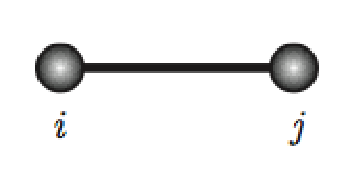
\includegraphics{figures/SpringForce}
  \caption{The spatial arrangement of particles for a \texttt{SpringForce}}
  \label{fig:springf}
\end{figure}

\subparagraph{RodBendingForce}

A RodBendingForce is a constraint force acting open three particles
that come to form a single hinge. The energy associated to the
rod-bending force depends upon the current angle $\theta$, as well as
some user-defined parameters: the undeformed lenghts of the edges
$\vec{ij}$ and $\vec{jk}$, the undeformed-angle $\bar{\theta}$, and
the force stiffness. The spatial arrangement of this force can be seen
in Figure \ref{fig:rodf}.

\begin{figure}
  \centering
  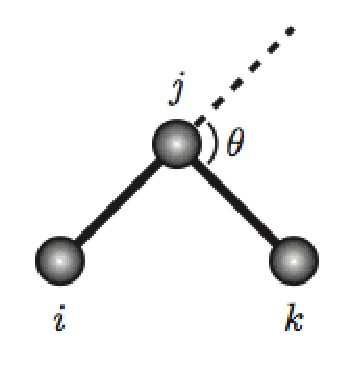
\includegraphics{figures/RodBending}
  \caption{The spatial arrangement of particles for a \texttt{RodBendingForce}}
  \label{fig:rodf}
\end{figure}

\subparagraph{TriangleForce}

The TriangleForce is based on a triangle stencil
involving three particles. This force resists both stretching and
compressing the triangular formation and depends upon the undeformed
lengths of the triangle edges, as well as the forces tensile modulus,
a measure of material stiffness, and its Poisson ratio, which relates
material compression to extraction. The spatial arrangement of this
force can be seen in Figure \ref{fig:trianglef}.

\begin{figure}
  \centering
  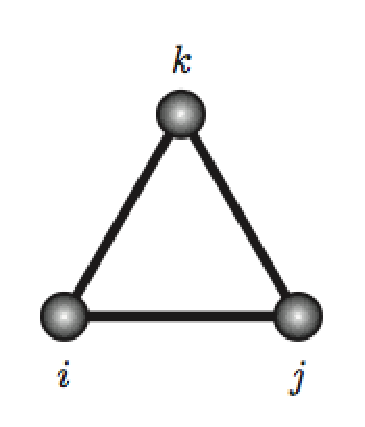
\includegraphics{figures/Triangle}
  \caption{The spatial arrangement of particles for a \texttt{ConstantStrainTriangleForce}}
  \label{fig:trianglef}
\end{figure}

\subparagraph{SurfaceBendingForce}

A SurfaceBendingForce is a constraint force that resists the bending
of a four-particle surface along its diagonal. The force energy is
based on the dihedral angle, $\phi$, which is the signed angle between
the normals of the two triangles in the configuration. The
SurfaceBendingForce class is thus parameterized by the undeformed
dihedralangle, the undeformed triangle edge lengths and the force
stiffness constant. The spatial arrangement of this force can be seen
in Figure \ref{fig:surfacef}.

\begin{figure}
  \centering
  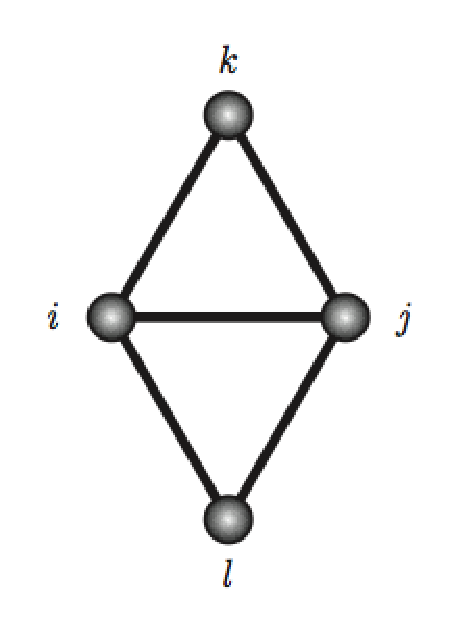
\includegraphics{figures/SurfaceBending}
  \caption{The spatial arrangement of particles for a \texttt{SurfaceBendingForce}}
  \label{fig:surfacef}
\end{figure}

\subsubsection{Properties}
Properties objects foremost include the non-optional properties of
simulation: time integration and rendering. Every simulation requires
a time-stepping method that defines force integration with each
update; and every simulation requires a method of outputting the
rendered scene. The property type can additionally be used to define
simulation features such as collision detection and response
frameworks, textures, lighting, and camera controls.

\paragraph{Predefined time integrators}

Feynstein provides two methods of integration, velocity Verlet and
semi-implicit Euler, for calculating changes to the scene over each
time step. Both the Verlet and semi-implicit Euler methods yield
more stable approximations of an object's trajectory than the explicit
Euler method, the other conventional method of calculation, which we
have omitted in the interest of accuracy. The integrators are defined
as \texttt{VelocityVerlet} and \texttt{SemiImplicitEuler} objects, and both require
only one parameter, the size of the time step to use in the time
integration calculations. This parameter should consist of a numerical
value and a time literal specifying the value's units.

\begin{verbatim}
properties {
  /* (other property declarations) */
  property SemiImplicitEuler(stepSize = 5ms);
}
\end{verbatim}

\paragraph{Predefined renderers}

Feynstein supports both online and offline methods of video output.
Online rendering means that when a Feynstein program runs, it displays
output directly on the screen. Online rendering produces an
interactive video output that lets the user use the mouse to change
the location of the camera, pan, tilt, and zoom during the
simulation. By default, Feynstein uses online rendering.  The use of
online rendering does not need to be explicitly specified.  If online
rendering is not wanted, how Feynstein should render the video needs
to be specified.  Offline rendering outputs a video file to a
specified file.

\begin{verbatim}
properties {
  property FileOutput(file="myScene.avi");
  property CameraView(location=(5m, 0, 0), 
    lookingAt=(0, 0, 0), fieldOfView=50);
}
\end{verbatim}

The user specifies where Feynstein should render the video using
the \texttt{FileOutput} property. The parameter of \texttt{File\-Output} is a
string specifying the file. Using offline rendering requires that the
camera position is specified using the \texttt{CameraView} property.

\paragraph{Predefined collision handlers}
Efficient collision detection and effective collision response are
essential to achieving accurate simulation for most scenarios. The
Feynstein language has built in property types for easy collision
detection and response.

\subparagraph{Detectors}

Feynstein supports a traditional, two-phase collision detection
framework. The narrow phase of detection supports both a basic proximity-based
method for classifying collisions, and more costly continuous-time detection for greater accuracy in
collision handling. To add a collision detection to your simulation, declare a
new \texttt{ProximityDetector} or \texttt{ContinuousTimeDetector} to the properties subsection. 

\begin{verbatim}                                                                                                                                             
properties {                                                                                                                                                 
  /*other property declarations...*/                                                                                                                         
  property ProximityDetector(proximity=1e-3);                                                                                                                
}                                                                                                                                                            
\end{verbatim}

\begin{description}
\item[ProximityDetector] A \texttt{ProximityDetector} requires one
  parameter: the minimum proximity that can be exhibited between two
  triangles before they are detected as colliding. At each simulation
  update, the \texttt{ProximityDetector} determines if any two
  triangles are going to violate this minimum proximity, and if so,
  marks them as colliding.

\item[ContinuousTimeDetector] A \texttt{ContinuousTimeDetector}
  requires no parameters and detects collisions at each simulation
  update by using each triangles current positions and velocities to
  determine at what time they would collide. If this collision time
  falls in between the current time and next update time, the two are
  marked as colliding.

  The optional broad phase of detection uses a spatial hierarchy, with
  support for a variety of bounding volumes, to determine pairs of
  triangles that are close enough to exhibit a collision. These
  potentially colliding triangles are then passed to the narrow phase
  detection, which would otherwise operate on the entire global
  mesh. This data structure is provided as an optimization to
  proximity-based collision detection and will automatically wrap all
  triangles in the global simulation mesh.

  To add broad phase detection to your simulation, declare a new
  \texttt{Bounding\-Volume\-Hierarchy} in the properties subsection of
  the Feynstein program. A \texttt{Bounding\-Volume\-Hierarchy}
  requires a bounding volume type specification: \texttt{AABB} for
  Axis-Aligned Bounding Boxes (default), \texttt{SPHERE} for Spheres,
  and \texttt{KDOP\_n} for n-degree K-Discrete Oriented Polytopes with
  $n \in {6, 14, 18, 26}$. Note that declaration of an broad phase
  detection property without a narrow phase detection property will
  cause a compiler error;

\begin{verbatim}
properties {
  /*other property declarations...*/
  property BoundingVolumeHierarchy(
    type=BoundingVolumeHierarchy.AABB, margin=1e-3);
  property ContinuousTimeDetector(stepSize=.01);
}
\end{verbatim}
\end{description}

\subparagraph{Responders}

Collision response is handled by an additional property. Feynstein
includes two methods for responding to collisions. The first method, \texttt{SpringPenaltyResponder},  is a penalty-based method that uses a \texttt{SpringForce} between objects to resist their impact. The second method, \texttt{ImpulseResponder}, applies iterative impulses to object's velocities until collisions converge. All collision responders take a detector instance as a parameter. This detector will feed the responder it's collision set.

\begin{verbatim}
 properties { 
	/* other property declarations... */
        property BoundingVolumeHierarchy(margin=0.1);
        property ProximityDetector(proximity=0.1);
        property SpringPenaltyResponder(detector=0, stiffness=1000, proximity=0.1);
   }
\end{verbatim}
\begin{description}
\item[SpringPenaltyResponder] The \texttt{SpringPenaltyResponder}
  takes two parameters in addition to it's detector index: Thie spring
  stiffness used to resist collisions and the minumum proximity
  allowed between two triangles (i.e. the rest length of the
  spring). \texttt{SpringPenaltyResponder} takes a set of collisions
  from it's detector, which are flagged one of two canonical collision
  types: \texttt{VERTEX\_FACE} (one vertex and a three-vertex face)
  and \texttt{EDGE\_EDGE} (two two-vertex edges).

  The two points of the standard \texttt{SpringForce} stencil are then
  computed using the barycentric coordinates of the contact points
  within a face or along an edge. In a sense, the
  \texttt{SpringPenaltyResponder} holds a sub-\texttt{SpringForce} for
  each exhibited collision vertex set.

\item[ImpulseResponder] An \texttt{ImpulseResponder} takes one
  parameter in addition to it's detector index: The maximum number of
  iterations to perform when modifying object velocities until
  collisions converge. At each iteration, the
  \texttt{ImpulseResponder} projects the simulation state forward in
  time by updating object velocities and asking its detector to check
  for collisions. If any are found, impulses (either elastic or
  inelastic) are applied to object velocities, and the future
  simulation state is recomputed with the new velocities. This
  iterative step is performed until all collisions disappear or some
  maximum number or interactions is reached.
\end{description}
\begin{verbatim}
 properties { 
	/* other property declarations... */
        property ProximityDetector(proximity=0.1);
        property ImpulseResponder(iterations=100, detector=0);
   }
\end{verbatim}


\paragraph{Camera Location and Orientation}

The CameraView property defines how the scene will appear to the
viewer. The location of the camera is given by a location (x, y, z) in
the scene. The camera has a default field of view of 45º, but this can
be changed when the camera is defined. By default, the camera is
located at the midpoint of the xy-projection of the objects in the
scene, and the default z value is calculated so that the camera can
see all objects in the scene.

\begin{verbatim}
properties {
  /*other property declarations */
  property CameraView(location=(0, 0, 3m), 
    lookingAt=(0, 0, 0), fieldOfView=30);
}
\end{verbatim}

\subsection{Execution Model}

\subsubsection{Code Blocks}
Code blocks consist of multiple statements executed as a group, and
the blocks can be nested. Code blocks are used to determine the
grouping of statements such as those that are part of a main Feynstein
code subsection or those that are part of a loop. The beginning of a code
block is delineated with a \texttt{\{}. The end of a code block is delineated
with a \texttt{\}}. Variables declared inside of a code block exist only
within that block of code.

\subsubsection{Stability Analyzers}

Stability analyzers are activated at run-time and throw exceptions
when the difference between the average kinetic energy at the
beginning of the simulation and the average kinetic energy at the
point in time being analyzed is not within the default tolerance
(1e-3), or a tolerance specified using the AssertStability property in
the properties block.

\begin{verbatim}
properties {
  /*other property declarations */
  property AssertStability(maxError=1e-6);
}
\end{verbatim}

\subsection{Grammar}

Note that, in the grammar below, the string \texttt{epsilon} is taken
to mean $\epsilon$, or the empty string.

\subsubsection{Tokens}

\begin{verbatim}
ID ::= (letter|'_')(letter | digit | '_')*
NUMBER ::= decimal
STRING ::= '(letter)*'

literal ::= timeLiteral | spatialLiteral 
            | massLiteral | forceLiteral
timeLiteral ::= day
day ::= decimal 'td' hour | hour
hour ::= decimal 'th' minute | minute
minute ::= decimal 'tm' second | second
second ::= decimal 'ts' millisecond | millisecond 
millisecond ::= decimal 'tms' | epsilon

spatialLiteral ::= meter | feet
	meter ::= decimal 'm' centimeter | centimeter
centimeter ::= decimal 'cm' millimeter | millimeter
millimeter ::= decimal 'mm' | epsilon
feet ::= decimal 'ft' inch | inch
inch ::= decimal 'in' | epsilon

velocityLiteral ::= spatialLiteral '/' timeLiteral | episolon

massLiteral ::= kilogram
kilogram ::= decimal 'kg' gram | gram
gram ::= decimal 'g' milligram | milligram
milligram ::= decimal 'mg' | epsilon

forceLiteral ::= decimal 'N' | epsilon

letter ::= lowercase | uppercase
lowercase ::= 'a'...'z'
uppercase ::= 'A'...'Z'
digit ::= '0'...'9'
decimal ::= pointfloat |exponentfloat
pointfloat ::= [intpart] fraction | intpart '.'
exponentfloat ::= (intpart | pointfloat) exponent
intpart ::= int+
fraction ::= '.' int+
exponent ::= ('e'| 'E') ['+'|'‐'] int+
\end{verbatim}

\subsubsection{File Structure and Expressions}

The following production describes the canonical organization for Feynstein files:
\begin{verbatim}
FeynsteinFile ::= ID { optCode shapeBlock optCode forceBlock 
  optCode propertyBlock optCode onframeBlock }
optCode ::= optcode statement | epsilon
\end{verbatim}
Feynstein-specific blocks, however, can appear in any order.

\begin{verbatim}
shapeBlock ::= 'shapes' '{' shapes '}'
shapes ::= shapes shape ';' | epsilon
shape ::= 'shape' 'Sphere' '(' sphereParams ')' 
  | 'shape' 'Cylinder' '(' shapeParams cylParams ')' 
  | 'shape' 'Plane' '(' shapeParams planeParams ')' 
  | 'shape' 'RectangularPrism' '(' shapeParams rectParams ')' 
  | 'shape' 'Tetrahedron' '(' shapeParams tetParams ') 
  | 'shape' 'Cube' '(' shapeParams cubeParams ')'
  | 'shape' 'FluidPlane' '(' shapeParams fPlaneParams ')'
  | 'shape' 'ParticleSet' '(' shapeParams pSetParams ')'
  | 'shape' 'ClothPiece' '(' shapeParams pSetParams ')'
  | 'shape' 'RegularPolygon' '(' shapeParams regPolyParams ')'
  | 'shape' 'SinglePointMass' '(' shapeParams pointMassParams ')'
  | 'shape' 'SpringChain' '(' shapeParams pSetParams ')'
  | 'shape' 'TriangleShape' '(' shapeParams triangleParams ')'
  | 'shape' ID '(' shapeParams userParams ')' 

shapeParams ::= 'name' '=' STRING
  | 'location' '=' point
  | 'velocity' '=' '(' NUMBER velocityLiteral ',' NUMBER velocityLiteral ',' NUMBER velocityLiteral ')'
  | 'mass' '=' NUMBER massLiteral
  | 'particleRadius' '=' NUMBER spatialLiteral
  | 'fixed' '=' NUMBER
  | epsilon

point ::= '(' NUMBER ',' NUMBER ',' NUMBER ')'

sphereParams ::= 'radius=' NUMBER spatialLiteral sphereOpt
sphereOpt ::= ',' 'accuracy' '=' NUMBER | epsilon

cylParams ::= height cylOpt ',' radius cylOpt 
  | radius cylOpt ',' height cylOpt
radius ::= 'radius' '=' NUMBER spatialLiteral
  | 'radius1=' NUMBER spatialLiteral ',' 'radius2=' NUMBER spatialLiteral 
height ::= 'height' '=' NUMBER spatialLiteral ',' cylParams
cylOpt ::= ',' 'accuracy=' NUMBER | epsilon

planeParams ::= planeParams 'normal '=' point

tetParams ::= 'point1' '=' point ',' 'point2' '=' point ',' 'point3' '=' point ',' 'point4' '=' point ','

cubeParams ::= 'sides' '=' '(' NUMBER spatialLiteral ',' NUMBER spatialLiteral ',' NUMBER spatialLiteral ')'
  | 'allSides' '=' NUMBER spatialLiteral

fPlaneParams ::= 'lengthX' '=' NUMBER spatialLiteral fPlaneOpt ',' 'lengthY' '=' NUMBER spatialLiteral fPlaneOpt
  | fPlaneParams 'length' '=' NUMBER spatialLiteral fPlaneOpt
fPlaneOpt ::= ',' 'subdivisions' '=' NUMBER | epsilon

pSetParams ::= vert pSetOpt
vert ::= vert 'vert' '=' point | epsilon
pSetOpt ::= ',' 'fixed' '=' NUMBER | epsilon

regPolyParams ::= 'vertices' '=' NUMBER ',' regPolyParams 'radius' '=' NUMBER spatialLiteral
  |  regPolyParams 'radius' '=' NUMBER spatialLiteral ',' 'vertices' '=' NUMBER

pointMassParams ::= 'pos' '=' NUMBER

userParams ::= userParams STRING '=' STRING 
  | userParams STRING '=' NUMBER 
  | userParams STRING '=' NUMBER literal
  | epsilon


forceBlock ::= 'forces' '{' forces '}'
forces ::= forces force ';' | epsilon
force ::= 'force' 'GravityForce' '(' gravityParams ')' 
  | 'force' 'DampingForce '(' forceParams dampParams ')' 
  | 'force' 'SpringForce' '(' forceParams springParams ')' 
  | 'force' 'RodBendingForce '(' forceParams rodParams ')' 
  | 'force' 'ConstantStrainTriangleForce '(' forceParams triangleParams ')' 
  | 'force' 'SurfaceBendingForce' '(' forceParams surfaceParams ')' 

forceParams ::= 'actsOn' '=' '#' STRING
  | epsilon

gravityParams ::= gravityParams 'gx' '=' NUMBER
  | gravityParams 'gy' '=' NUMBER
  | gravityParams 'gz' '=' NUMBER
  | epsilon

dampParams ::= 'coefficient' '=' NUMBER | epsilon

springParams ::= springParams 'length' '=' NUMBER spatialLiteral
  | 'strength' '=' NUMBER
  | epsilon

triangleParams ::= 'youngs' '=' NUMBER ',' 'poisson' '=' NUMBER

rodBendingParams ::= rodBendingParams 'strength' '='  NUMBER
  | rodBendingParams 'angle' '=' NUMBER
  | epsilon

surfaceBendingParams ::= 'strength' '=' NUMBER | epsilon

propertyBlock ::= 'properties' '{' properties '}'
properties ::= properties property ';' |  epsilon
property ::= 'property' 'renderTo' '(' renderParams ')' 
  | 'property' 'endTime' '(' endParams ')' 
  |  'property' 'assertStability' '(' assertParams ')' 
  | 'property' eulerMethod '(' eulerParams ')' 
  | 'property' 'CameraView' '(' cameraParams ')' 
  | 'property' 'ProximityDetector' '(' 'proximityParams' ')' 
  | 'property' 'ContinuousTimeDetector' '(' cTParams ')'
  | 'property' 'BoundingVolumeHierarchy' '(' 'bvhParams' ')'
  | 'property' 'SpringPenaltyResponder' '(' springPenaltyParams ')'
  | 'property' 'ImpulseResponder' '(' impulseParams ')'

renderParams ::= 'VideoOutput' | 'FileOutput' '(' STRING ')' | epsilon

endParams ::= 'endAt' '=' timeLiteral | epsilon 

assertParams ::= epsilon | 'margin=' NUMBER 

eulerMethod ::= 'VelocityVerlet' | 'SemiImplicitEuler'
eulerParams ::= 'stepSize' '=' timeLiteral

cameraParams ::= 'location' '=' '(' NUMBER ',' NUMBER ',' NUMBER ')'
  ',' 'lookingAt' '=' '(' NUMBER ',' NUMBER ',' NUMBER ')' 
  ',' 'fieldOfView' '=' NUMBER

proximityParams ::= 'proximity' '=' 'NUMBER'

bvhParams ::= 'margin' '=' NUMBER | 'margin' '=' NUMBER ',' 'type' '=' 'BoundingVolumeHierarchy.' 'volumeType'
volumeType ::= 'AABB'

springPenaltyParams ::= 'proximity' '=' NUMBER springOpt ',' 'detector' '=' NUMBER springOpt
  |  'detector' '=' NUMBER springOpt ',' 'proximity' '=' NUMBER springOpt
springOpt ::= ',' stiffness' '=' NUMBER 

impulseParams ::= 'iterations' '=' NUMBER ',' 'detector' '=' NUMBER 
  | 'detector' '=' NUMBER ',' 'iterations' '=' NUMBER
  | 'detector' '=' NUMBER

onFrame ::=  'onFrame ' '{' onFrameAxns '}' | epsilon
onFrameAxns ::= statements statement | epsilon

statements ::= expression statements | statement statements | epsilon
statement ::= ID '=' expression | ID '=' tok
tok = ID | NUMBER | shape | force | property | timeLiteral
	expression ::= arithOperation | compOperation | boolOperation

arithOperation ::= NUMBER binOp NUMBER | '-' NUMBER
binOp ::= '+' | '-' | '/' | '*' | '%' | '^'

compOperation ::= NUMBER compOp NUMBER | ID '==' ID
compOp ::= '==' | '!=' |'>=' | '<=' | '>' | '<'

boolOperation ::= boolean boolOp boolean
boolean ::= 'TRUE' | 'FALSE' | compOperation | boolOperation
boolOp ::= 'and' | 'or' | '!'

conditional ::= 'if (' boolean '){' statements '}' elseBlock 
  | 'while (' boolean ') {' statements '}' 
  | 'do {' statements '} while (' boolean ');' 
  | 'for (' forInit ';' forExpr '; forUpdate ') {' statements '}'

elseBlock ::= 'else if (' boolean ') {' statements '} elseBlock 
  | 'else {' statements '}' | epsilon

forInit ::= expression | varDeclaration | epsilon
forExpr ::= expression forExpr | expression | epsilon
forUpdate ::= expression forUpdate | epsilon

\end{verbatim}

}{}

\section{Project Plan}
\emph{Colleen McKenzie, Project Manager}

\subsection{Development Process}
Two aspects of our development process that I believe contributed to
the project’s success were the modularity of our language and compiler
and our decision to build our language and our code base in
increments. There were, of course, general aspects of the language
that had to be decided on early in the project, such as the
overarching structure of a Feynstein file, and these were discussed
and voted on at group meetings. Our Language Guru defined a hierarchy
of discrete features for inclusion, so that we could start out with a
small but functional code base and build on it to include as many
possibilities as possible for our languages users. (See section on
Language Evolution for an in-depth description of this process.)
Because we divided our language into sections in accordance with
physical elements--there are shapes (masses), forces, and properties
such as time integration and collision handling--the modules of our
translator could be designed, developed, and tested independently of
each other, which decreased the dependencies in our language and
allowed the maximum flexibility for group members to work at their own
paces to finish the sections of the project assigned to them.

\subsection{Roles and Responsibilities}
While our language was modular and easily separated into discrete sections,
the responsibilities of the project's group members were far less
distinct than we expected and than the course materials' guidlines
suggested they be. I believe this unsystematic distribution of work
speaks to the flexibility of our project group, but certain areas of the
project may have run more smoothly if we had made firm decisions
about what our group roles constituted early in the course of the project.

\begin{description}
\item[Colleen McKenzie: Project Manager] I was responsible for
  organizing meetings and taking minutes at group meetings. I also
  handled updating the group’s project wiki and Google Calendar with
  minutes, resources, events and deadlines, and other changing 
  information pertaining to our language and its
  implementation. Monitoring group members’ progress was also my
  responsibility, and I regularly checked in with group members to
  keep track of progress in each contributor’s area of language
  development and implementation. This monitoring also included the
  setting (and resetting) of deadlines and querying group members
  about their progress. Finally, I was responsible for proofreading
  all documentation (typeset by our Systems Architect) and either 
  correcting errors or communicating issues to the Language Guru.

\item[Samantha Ainsley: Language Guru] Samantha was responsible for
  providing the conceptual organization of the language--she was our
  essentially our Physics Guru, and she used her expertise to lead us
  to consistent and logical decisions about the design of our
  language. She provided reference materials to give us an idea of how
  other languages and libraries implemented functionality similar to
  Feynstein’s and was the designated point person for questions
  related to such matters. Further, Sam was largely responsible for
  executive decisions about which features our language would and
  wouldn’t support.

\item[Will Brown: Systems Architect] Will was responsible for defining
  the structure of the Feynstein compiler code package, which is
  broken up into modules for translation and for processing different
  simulation aspects. In addition, Will was entirely responsible for
  the translation portion of the compiler: he worked with our Language
  Guru’s design to ensure that our language was properly translated
  into Java code built on the compiler architecture he designed. Will
  also managed the repository for the group’s code and managed the
  documentation process: he was responsible for compiling and
  typesetting all of our group's written material.

\item[Rob Post: Systems Integrator] Rob was responsible for
  researching information we used to design and add features to our
  rendering module, and make decisions about what features and options
  for visual output we would provide users of our language. Rob also
  collaborated with the Systems Architect to implement robust
  compile-time error handling in our translator.

\item[Eva Snow: Tester and Validator] Eva was responsible for
  implementing unit tests designed to make sure our language properly
  supported all the features defined in our manual and ensuring that
  the physical features of our language had been implemented
  correctly.
\end{description}

\subsection{Implementation Stylesheet}
Our group did not have an implementation stylesheet. Our development
process included group members reading through project code before
contributing more, and because our Language Guru and Systems Architect
defined a robust API while laying the groundwork for the compiler,
members contributing new modules were able to sufficiently match the
project’s existing code.

\subsection{Project Timeline}
\begin{description}
\item[1/24] We decided on and assigned roles for each team member,
  made logistical decisions (e.g. weekly meetings), and decided on
  physical simulation as the domain for our language.

\item[1/30] Group members gained familiarity with the language domain,
  including higher-level physical concepts we would need to implement.

\item[2/6] We developed and recorded milestones for our project and
  started working on a general language specification to guide future
  language developments and additions.

\item[2/13] With a few tweaks, we made our earlier language
  specification final. By this point our builder syntax is
  well-defined.

\item[2/20] Our language whitepaper is finished at this point.

\item[2/27] We defined more specific milestones for implementing the
  compiler, and we identified and accounted for dependencies in the
  structure of the language and the compiler.

\item[3/29] By this point, the language reference manual and tutorial
  were complete. We had a solid specification and a grammar for our
  language, both of which were very close to the grammar of our
  finalized language.

\item[4/3] Translation for Feynstein-specific syntax was implemented,
  and early translator testing was implemented alongside the
  translator. Our git repository was up and running, and all members
  were able to commit code. We implemented basic functionality of our
  renderer so that it could could display a basic shape to the
  screen. Mouse and keyboard commands were implemented with the
  rendered so that users could change the view of their scene.

\item[4/10] Automated compilation and running of Feynstein files was
  implemented by this point. The modules in our compiler were divided
  up discretely among group members.

\item[4/18] Time-stepping was implemented, but not integrated into
  Feynstein yet.

\item[4/24] We implemented basic discretization of geometry: at this
  point we had fully functional objects in our language, and these
  could be operated on by force constructs. Basic forces (gravity,
  springs) were also implemented.

\item[5/3] All forces were implemented by this point.

\item[5/5] Basic force testing was completed and collision detection
  was implemented by this point.

\item[5/6] Collision response was implemented, and the translator was
  extended to handle errors in more specific and descriptive ways.
\end{description}
\subsection{Project Log}
Please see Appendix \ref{sec:projectlog} for the (rather lengthy)
project log.


\section{Language Evolution}
\emph{Samantha Ainsley, Language Guru} \\

The Feynstein language evolved rather smoothly throughout the course
of this project. From the very beginning we agreed upon a syntax and
feature set for our language. We defined a set of clear milestones
that we then organized into a language pipeline. Naturally, our first
goal was to have our parser and syntax interpreter up and running, so
our execution code could be written with few changes to the translator
and interpreter. After this, our second milestone was to implement our
renderer, without which no testing could be performed as Feynstein
requires visual display. Both of these hurdles were overcome in the
first half of the semester. With this foundation established, we were
able to divide our language into independent features and assign
development accordingly.

The dependency graph shown in Figure \figref{depend} shows the work
flow for our language development. An arrow indicates a dependency,
i.e. if A->B, then A must be completed before B. Features shown in
italics were deemed second priority because no other language modules
depend upon them and they are not necessary for testing, or there
exists an equivalent feature. Based on this flow graph, we decided to
assign integration and shapes to different team members as they could
clearly be completed in parallel. The team member responsible for
integration would first complete one integrator before developing an
additional integrator, so the person responsible for forces could
begin their work. The person responsible for forces would first
complete spring forces, as collision response will depend on this
logic (and it is the simplest force potential). Forces where An
additional person would then be responsible for handling collisions,
which we agreed upon as a second completion state. As collision
detection extends all other primary modules, it could be left for
future development with the language in a completed state under
undesirable circumstances.

\imgfig{depend}{.5}{Dependencies in Feynstein}{depend}

Our syntax, which is intentionally close to Java for easy integration
of Java code into Feynstein programs, improves upon Java with a
feature we called Builder Syntax. Builder Syntax allows users to
specify Feynstein object instantiation parameters in an arbitrary
order with key-value pairs. For example, a user creates a gravity
force as \code{force GravityForce(gy=-9.8)}. The GravityForce takes
additional optional parameters gx, and gz, which specify the
acceleration due to gravity in the x and z directions,
respectively. This important feature makes Feynstein accessible to
users without requiring an in-depth understanding of its API.

The systems architect took primary responsibility for developing the
translator logic of Builder Syntax translator was completed in the
first half of the project timeline. Meanwhile, the language guru wrote
the OpenGL pipeline render as a stand-alone Java application to be
incorporated into the make Feynstein program. The architect's Builder
Syntax implementation allowed for each development of new-key value
pairs without modifying the basic grammar. Instantiation parameters
are configured as a chain of function calls, each of which returns the
updated object instance. The syntax was also developed to support list
configuration when setting multidimensional parameters; for example,
\code{shape Sphere(position=(0.0,0.2,0.2))}. Builder Syntax keys
translate to methods of name \code{set\_<key\_name>} that return an
instance of the class type--this facilitated rich feature development
for the rest of the team.

With the goal of allowing the team to easily develop properties,
shapes, and forces independently, our architect wrote the APIs for
each base class. With our code checked into a central repository, the
other team members could fill in the method logic
accordingly. Geometric primitives were developed for the renderer and
used to build a triangle mesh class for shape topology. As planned, we
developed our initial custom shapes in parallel with the Semi-implict
Euler integrator. We implemented the .obj file parser first, as this
would allow for quick render testing without defining complex
geometric configurations dynamically. We then developed forces while
extending our custom shape library. Forces were developed in order of
increasing complexity measured in the number of particles they act
upon. The most complex force we aspired to support, a tetrahedral
constraint force, was omitted from the language as it only applied to
a single shape configuration. We developed particle-interpolation
shapes, which are small shapes defined by a list of vertices, in light
of forces for easy unit testing of force stencils.

We had hoped to develop a second time integration class in parallel to
force and shape development, but did not reach this goal. The
ImplicitEuler method we hoped to support required a complex
multi-dimensional numerical solver for which we could not find an
appropriate external library. We did however, add a less complex
Velocity-Verlet based integrator to offer users more flexibility. We
completed all force and shape definitions soon enough that we could
focus our last efforts towards building our collision detection system
while simultaneously developing a syntactical feature that allowed
users to manipulate shapes with predefined operators. We first
completed proximity-based collision detection, then continuous-time
collision detection, which is significantly more complicated and
precise. We then developed a penalty-spring-based collision handler
followed by an impulse-based handler.

With the exception of our two minor changes, our language evolved
beyond our first completion stage. We achieve our milestones on time,
though sacrifices in division of labor often had to be made to reach
this goal. With better deadline achievement, I believe we could have
achieved more interesting rendering capabilities into the
languages--such as lighting and textures. Nevertheless, our final
feature set provides a rich framework for configuring physics-based
simulation as well as many easily-extendable building blocks for
future research and development.


\section{Language Architecture}
\emph{William Brown, System Architect} \\

The Feynstein system is broken into two distinct portions; the
translator and the Feynstein execution environment. The translator
takes, as input, Feynstein source code and translates it into valid
Java source code. This Java code is then run in the Feynstein
execution environment, which pulls in all of the Java code we have
written to provide the rendering, geometry and simulation constructs
that are present in Feynstein.

\subsection{Translator}

The translator uses a multi-pass system to translate Feynstein into
Java. It first does basic lexing, in which it breaks inputs first into
statements, then into the lexemes within those statements. After
lexing, it constructs a syntax tree. Once the code exists within this
tree, the translator walks the tree to generate valid Java code. In
most cases, this is simple textual substitution; for example, the
Feynstein code segment \code{\#myShape} translates directly into
\code{getShape(``myShape'')}. However, some constructs require a more
in-depth parsing; in particular, builder syntax was quite difficult to
translate. These statements, of the form
\code{MyObject(attribute1=value, attribute2=value)}, were not valid
Java and thus didn't cause a collision in our grammar, but still were
difficult to distinguish from, say, \code{MyObject(x == y)}, which is
valid Java (if \code{MyObject} takes a boolean as an argument to its
constructor).

We do have one unusual step in our translator, which is ``structure
analysis'' -- since Feynstein has certain parts of the language which
this user is required to use (for example, the user must specify a
``shapes'' block), we analyze the syntax tree to ensure that they've
incorporated the required portions of the source code.

Error handling in Feynstein is difficult; we need to handle errors
returned by the Java compiler and virtual machine and give users some
indication as to where in their original Feynstein (instead of the
generated Java code) the error occured. To do so, during parsing and
syntax analysis we generate a mapping of Java line numbers to
Feynstein line numbers. Then, if the Java compiler or VM throws an
error, we mine the stack trace for the Java line number which causes
the error and tell the user which line number in Feynstein generated
that Java code.

Both Rob and Will contributed to the translator. Will wrote the
initial implementation of the translator and was responsible for
implementing new features at the translator level. Rob was responsible
for error handling.

A block diagram of the translator is shown in \figref{translator}

\imgfig{translator}{.8}{Block diagram of the stages in the
  translator}{translator}

\subsection{Execution Environment}

The execution environment of Feynstein is the more complex half of the
system; while our language is very similar to Java and therefore
requires simple translations, the actual behavior of a Feynstein
program is extremely complex. This complexity is mirrored in the
complexity of the architecture in the two portions; while the
translator had four modules and a fairly simple API, the execution
environment is composed of almost 7000 lines of Java code split across
50 classes. A block diagram of the execution environment is shown in
\figref{eeblock}.

Will defined the API for the components in the system to ensure
consistency and compatibility with translator output. From a
high-level implementation perspective, Sam was responsible for
renderer, geometry and forces, Colleen was responsible for collisions
and integrators, and Will was responsible for shapes. For a more
in-depth summary of who was responsible for what, see Appendix
\ref{sec:whowhat}, and for a line-by-line listing of who wrote what
code, see Appendix \ref{sec:listing}.

\imgfig{eeblock}{.35}{Block diagram of the execution environment
  architecture}{eeblock}

\section{Development Tools}
\emph{William Brown, System Architect}

\subsection{Source Code Management}

In order to manage our team's source code, we used Git, which is a
distributed version control system. Will set up a Git repository on
his server, to which everyone on the team was given SSH access. It
allowed all of us to simultaneously work on Feynstein and then easily
merge our changes together. Git also allowed us to easily track
peoples' contributions to the code base, as it allows a user to see
exactly who wrote each line of code in a repository. Will wrote a
shell script that allowed us to see exactly who wrote how much, as
well, which helped for the final calculations to ensure that everyone
had written at least 500 lines of code.

\subsection{Languages, Tools and Libraries Used}

We wrote our execution environment in Java, as this was the only
language with which the entire team was familiar. It also provided us
with the portability inherent in Java, which was important for a team
of two Mac users, a Windows user and two Linux users.

We make heavy use of OpenGL for our graphics, however, there isn't a
native OpenGL implementation in Java, as it requires many
``bare-metal'' computations that aren't possible in a virtual
machine. Instead, we used Java OpenGL\footnote{
 \url{http://jogamp.org}} (or ``JOGL''), which uses JNI to call native
C libraries on the machine. JNI is notorious for being difficult to
set up, and JOGL lived up to this expectation; while we found it was
easy to install for the members of our team who use Linux, it was
extremely difficult to install on OSX. 

However, the installation procedure was worth it; JOGL gave us the
full power of OpenGL, and allowed us to use OpenGL at near-native
speeds and efficiency. Without it, this project would not have been
possible.

On the translator side, we used
PLY\footnote{http://www.dabeaz.com/ply/} (Python Lex-Yacc) for lexing
and parsing. We wanted to use an implementation of Yacc in a scripting
language, as most of the actions in our parser were string
manipulations, and string processing tends to be easier in scripting
languages. We used Python as this is what Will and Rob were more
familiar with.

\section{Testing Plan}
\emph{Eva Asplund, System Tester} \\

Because there are so many components to Feynstein above and beyond
merely translating the code, much of the testing methodology was
geared towards validating the implementation of the physics of the
program. Testing for these elements involves rendering actual scenes
written in Feynstein in order to visually verify that the math in the
code is working. The Feynstein tests for built-in forces were modelled
after XML files used by Sam Ainsley in her physical simulation
project. As new forces and physics functions are added to the program,
the suite of visually-verifiable test programs can expand accordingly,
and is re-run in order to assure that the new code has not caused an
unintended change in the functioning of the old.

The Feynstein translator test consists of a Feynstein source code and
corresponding output in java. By running the code through a new
version of the translator and saving it before it is compiled and run,
one can verify that the new translator performs equivalent
transformation. Once this new output is compiled and executed to
ensure its validity, it can be saved as the test for the next
generation Feynstein translator.


\section{Conclusion}
\subsection{Team Lessons}
We discovered the importance for having a central repository for all
updates to our grammar, of which there were many and which were often
communicated between members of the group instead of being recorded.

We learned the importance of defining general responsibilities in
advance: our roles were far less discrete than we expected them to be,
and while this is indicative of the cooperative way we approached this
project, it led to an unequal division of work that could have
possibly been avoided.  

We learned that the more modular our language was, the easier it was
to add--and remove--language components easily. 

\subsection{Individual Lessons}
\begin{description}
\item[Colleen: Project Manager] My belief in the validity of
  Hofstadter's Law--"It always takes longer than you expect, even when
  you take into account Hofstadter's Law"--has been confirmed many
  times over in the course of this project. I've learned a lot about
  the importance of setting realistic deadlines, but I've realized
  that it's equally important to accept that sometimes a schedule you
  thought was realistic at first needs to be radically changed.

  On a more individual note: I also learned the importance of understanding
  different styles of communication and of figuring out how one's team
  members work best: I believe that a few pitfalls could have
  been avoided if I had worked on our group's communication practices
  earlier in the project timeline. I initially approached the project as
  a very lenient manager, assuming that my group members--myself
  included--would produce work perfectly and according to schedule. I
  learned quickly that expecting people to behave as predictably as
  machines was unrealistic, and I began to understand the importance
  of instating policies for unfavorable situations at the
  beginning of the project, rather than once those situations have
  already happened.

  For our group, these situations mostly involved missed deadlines and an
  ensuing redistribution of work to the group members most able and willing
  to complete it. I began the project with the goal of giving all
  group members considerable enough contributions that they would
  all feel a sense of ownership for the project, but ultimately this
  was now how our group functioned, and I learned that at a certain
  point it's necessary to assign work to whoever will get it done
  quickly. A closely related lesson--and the hardest one for me to
  accept--was that sometimes the Project Manager has to prioritize
  completing a project over being nice or trying to keep everyone happy.

\item[Sam: Language Guru] Working on this language was fascinating for
  me, especially in a group dynamic. I proposed this language idea to
  my teammates because physical simulation is my primary area of
  research. The idea was very much inspired by my own experience
  learning simulation. I took a course in physical simulation that was
  taught entirely in C++, a language I was unfamiliar with at the
  time. I found (and I was far from alone) that most of my energy was
  put towards learning to use a new language in a very complex way:
  building an interactive object-oriented system and optimizing for
  performance. Although this was a great learning experience, within
  that particular course, I wished I could have focused more on
  understanding the physics behind the engine I was writing rather
  than just getting it to work--so much time was spent on the initial
  implementation that little was left for
  experimentation. As a result, I was inspired to create a language
  that facilitated easy understanding of the physical simulation
  concepts, but also allowed for more complex extension and
  experimentation.

  Needless to say, there was great pedagogical merit in this
  process. I am interesting in learning how different people
  understand the task of programming physical systems, and this gave
  me great insight. The language design is very much a reflection of
  this pedagogical experience. The act of teaching new concepts
  involves abstracting the lower level details into comprehensible
  objects and relationships. That said, my initial lessons for
  teaching simulation to the team ended up defining our language
  model. Furthermore, by working in Java, I learned a great deal about
  adapting my own perspective of developing simulation code, which is
  characterized by C++, to new languages--especially in terms of
  achieving optimal performance.

  Simulation aside, another important lesson I learned is about the
  dynamics of team work. In past experience, I have always tried to
  divide up labor as efficiently as possible so the maximal number of
  components could be developed in parallel. This division of labor
  was always straightforward when each person considered themselves a
  unique specialist. But what if not everyone is a specialist? I our
  group, there were some members who came in knowing exactly what they
  wanted to do, and others who were more flexible. There is, of
  course, an appeal to the person who is willing to work on anything,
  but from what I have learned, if someone considers themselves an
  expert, they will perform accordingly. I think that passion makes a
  team, and team members need to really to be confident in their
  necessity within the larger group from the beginning. I've learned
  that when selling an individual vision to a group of teammates, you
  should be certain each person is excited about their role.
	
  On that same token, one of the hardest parts of the language guru's
  job is letting go of control. When you envision a perfect system,
  you can't imagine accepting outside input. In some cases, my
  teammates showed me their clever and new perspectives on methods
  with which I've become rather familiar with developing
  simulators. It was admittedly hard to assign major coding components
  with which I was so familiar to my teammates. Some team members were
  very responsive, and I enjoyed collecting relevant reading materials
  to help them understand larger concepts, helping them through the
  coding process, and seeing their genuine excitement when things were
  working. Unfortunately, in other cases I believe some tasks may have
  been too daunting for team members. In these cases, I learned that
  you have to be aggressive when offering help--people won't always
  ask for it. On the other side, I also learned that sometimes you
  need to be resolute and put the language first, even if that means
  redistributing the work load towards those who consistently complete
  their work on time.

\item[Will: System Architect] I learned the value of defining APIs
  early on, because just the definition of an API is enough to get
  everyone thinking about how exactly things work. We had some issues
  later in the semester in which things couldn't work as we had
  planned, and we would have realized that that was the case if we had
  defined just what methods and fields each class in our execution
  environment had.

  I also learned (from experience) why everyone uses parser generators
  like YACC; at first, I tried to implement our language in pure
  Python, starting from scratch. I found that this approach made it
  much easier to write the actions in the SDTS for our language, but
  it made it extremely difficult to adapt to changes in our language's
  grammar.

  Finally, I learned a lot about my own division of labor when it
  comes to working in a team. Specifically, I found that the most
  challenging part of the project was responding to emails and
  maintaining the administrative part of the project; the coding came
  comparatively easily, despite the fact that I did a lot of
  coding. In fact, the largest headaches came from my job managing the
  documentation -- compiling everyone's contributions, ensuring that
  things got done on time and responding to people's requests for
  edits in a timely fashion were probably the most difficult tasks
  that I had.

\item[Rob: Systems] During this project, I learned two things. The
  first and probably most important thing I learned is that
  communication is essential in successful group work. I learned
  that I do not do this well and that it is something I need to
  improve upon if I want to be a more successful and productive group
  member in the future. The second thing I learned is that starting to
  code early is also really important in getting the best results as
  possible. It allows time to revise the code and make sure it works
  properly. That is also something which I will need to work on.

\item[Eva: Testing] You never know how much you're going to miss a
  debugger until it isn't there anymore.  It's pretty amazing the
  amount of knowledge contained in the heads of 5 Computer Science
  majors, but it's only helpful if you're asking questions.  Teammates
  and classmates can be a great resource, but only when you take the
  initiative to communicate and ask questions.
\end{description}

\subsection{Advice for Future Teams}
We found the existence of our team wiki to be very helpful, and would
encourage other groups to implement their own and use it even more
extensively than our group did. We would suggest that other groups
make sure that the basic framework for working together on a coding
project is in place early in the project. This framework would include
expectations about meetings and communication in addition to tools to
store, update, and communicate about the compiler's code at all stages
of the project. There are few replacements for effective
communication; in some cases, team members missed deadlines just
because their teammates didn't respond to emails in a timely
manner. Starting early and communicating effectively are both key to
meeting deadlines with high-quality results.

We also would advise future teams to set as many bail out points as
possible. Define versions 1.0, 1.1, and 1.2 of your language. Aspire
for version 1.2, but be willing to accept 1.0. This was definitely the
saving grace of our design process: we had many small
milestones. Also, it is important to never hesitate to ask team
members for help. This was definitely a struggling point for our
team. Remember that asking for help isn't a reflection of a lack of
intelligence, and more communication between teammates is always a
good thing. Getting stuck and not telling anyone is never an excuse
for failing to meet a deadline. On that same note: meet and meet
often. Lastly, be certain from the very beginning that every team
member knows the answer to these three questions: what is their role,
why were they chosen for it in particular, and are they excited about
it?

\subsection{Instructor Feedback}
\begin{description}
\item[Sam] I found the material for this course to be as interesting
  as it was difficult to grasp. My first suggestion would be more
  consistent written homework--however small--to reinforce ideas as
  they are learned. I would also suggest more consistency between
  homework and exams. I found that whereas the homework were more
  procedural, deriving from examples in the book, the exams were more
  conceptual.

  As far as the project is concerned, I would suggest a clearer
  definition of the five roles from the beginning. I remember our team
  did not gain a clear understanding of the distinction between the
  systems architect and integrator until the final report descriptions
  were posted. On that note, I often found that project-related
  assignments, such as the white paper and the language manual, did
  not come with explicit description. Perhaps more lessons focusing on
  the language design process would be beneficial.

\item[Colleen] I found the sections on run-time environments (chapter
  7) code generation (chapter 8) to be particularly interesting--both
  gave me a far greater understand of facets of computer programming
  that I had previously taken for granted. 

  As my group's project manager,
  I also loved Bob Martin's presentation on software projects, but I would
  have appreciated the information even more early in the semester, before
  I had already run into some of the problems he warned us about. In general,
  I would have liked to see  more information about project group roles and 
  advice about potential pitfalls early in the semester.

\item[Will] I really enjoyed all of the material associated with this
  course, and I think the project really gave me an appreciation for
  compilers and compiling tools. If I were to change one thing about
  this course, it would be to make homeworks more frequent. I would
  have liked to have more opportunities to apply some of the knowledge
  that I learned in lecture. Also, I'm not sure if this is unique to
  our language or all teams' languages, but we never got into any code
  optimization in Feynstein. I would have found a homework that
  required me to implement some basic code optimization really
  challenging and enjoyable.

\item[Eva] I think we covered grammars and regular languages a little
  more extensively than we needed to given that they were review. It
  would have been nice to get to YACC and lex right away.

\item[Rob] For future classes, I'd like to see a bit more examples of
  other programming languages and syntax styles, for no other reason
  other than I think things like that and I think it would be
  interesting and entertaining.
\end{description}


\startappendix

\section{Project Contributions}
\label{sec:whowhat}
\subsection{Contribution Summary}
\begin{table}[h]
  \centering
  \begin{tabular}{cl}
    1695 & Colleen McKenzie \\
255 & Eva Asplund \\
55 & Rob Post \\
4469 & Samantha Ainsley \\
2257 & Will Brown \\

  \end{tabular}
  \caption{Code contributions (in lines) by contributor}
  \label{tab:contrib}
\end{table}

\subsection{File-Level Breakdown}
\begin{description}
\item feynstein
  \begin{description}
  \item Built.java (Will)
  \item ClassGetter.java (Will)
  \item forces
    \begin{description}
    \item DampingForce.java (Sam)
    \item Force.java (Sam, Will)
    \item GravityForce.java (Sam)
    \item RodBendingForce.java (Sam)
    \item SpringForce.java (Sam)
    \item SurfaceBendingForce.java (Sam)
    \item TriangleForce.java (Sam)
    \end{description}
  \item geometry
    \begin{description}
    \item Edge.java (Sam)
    \item Mesh.java (Sam) 
    \item Particle.java (Sam)
    \item Transform.java (Will)
    \item Triangle.java (Sam)
    \end{description}
  \item properties
    \begin{description}
    \item collision
      \begin{description}
      \item AxisAlignedBoundingBox.java (Will) 
      \item BoundingVolumeHierarchy.java (Will)
      \item BoundingVolume.java (Will)
      \item Collision.java (Colleen)
      \item CollisionResponder.java (Colleen)
      \item ContinuousTimeDetector.java (Colleen)
      \item DistanceFinder.java (Colleen)
      \item ImpulseResponder.java (Colleen)
      \item NarrowPhaseDetector.java (Colleen)
      \item ProximityDetector.java (Colleen)
      \item SpringPenaltyResponder.java (Colleen)
      \item TrianglePair.java (Colleen)
      \end{description}
    \item integrators
      \begin{description}
      \item Integrator.java (Sam, Will)
      \item SemiImplicitEuler.java (Sam)
      \item VelocityVerlet.java (Sam)
      \end{description}
    \item Property.java (Sam)
    \end{description}
  \item renderer
    \begin{description}
    \item Renderer.java (Sam)
    \end{description}
  \item Scene.java (Colleen, Sam, Will)
  \item shapes
    \begin{description}
    \item ClothPiece.java (Sam)
    \item Cube.java (Will)
    \item CustomObject.java (Sam)
    \item Cylinder.java (Will)
    \item FluidPlane.java (Will)
    \item ParticleSet.java (Sam)
    \item Plane.java (Will) 
    \item RegularPolygon.java (Will)
    \item Shape.java (Will)
    \item SinglePointMass.java (Sam)
    \item Sphere.java (Will)
    \item SpringChain.java (Sam)
    \item Tetrahedron.java (Will)
    \item TriangleShape.java (Sam)
    \end{description}
  \item utilities
    \begin{description}
    \item ObjParser.java (Sam)
    \item Vector3d.java (Sam, Will)
    \end{description}
  \end{description}
\item translator
  \begin{description}
  \item blocks.py (Will)
  \item compile.py (Will, Rob)
  \item imports.py (Will)
  \item main.txt (Sam)
  \item matchers.py (Will)
  \item parse.py (Will, Rob)
  \item syntax.py (Will)
  \item translate.py (Will)
  \item translator.py (Will, Rob)
  \item units.py (Will)
  \end{description}
\item tests
  \begin{description}
  \item cantilever.f (Sam)
  \item collide.f (Will)
  \item collision
    \begin{description}
    \item ee1.f (Colleen)
    \item ee2.f (Colleen)
    \end{description}
  \item compile.f (Will)
  \item custom.f (Will) 
  \item gravity.f (Sam)
  \item initvel.f (Will)
  \item ops.f (Will)
  \item particlevelocity.f (Sam)
  \item properties.f (Will)
  \item rodbending0.f (Eva)
  \item rodbending1.f (Eva)
  \item rodbending1\_vv.f (Sam)
  \item rodbendingforce.f (Sam)
  \item shapetests.f (Will)
  \item springforce0.f (Eva)
  \item springforce1.f (Eva)
  \item springforce.f (Sam)
  \item surfacebendingforce.f (Sam)
  \item test.f (Will)
  \item transtest.f (Eva)
  \item triangle.f (Sam)
  \item velocityverlet.f (Sam)
  \end{description}
\end{description}

\section{Project Log}
\label{sec:projectlog}
\subsection*{1/24}

Meeting minutes ended up just being a to-do list. (Make a wiki, make a
git repository, everyone read Sam's notes, I’ll create pltphb@gmail
and start a calendar, we need a fifth group member).  

\subsection*{1/30}

Orders of business:
\begin{enumerate}
\item Meetings are Sundays, 8:30, Sam's suite. 
\item Everybody should read Sam's modeling papers for next week and
  send her whiny emails if they don't make sense.
\item Everybody should also read the git tutorial that Will is going
  to send/post on the wiki.
\end{enumerate}

Also:
\begin{itemize}
\item Will, do you want to just make everyone wiki accounts now so we
  don't have to deal with it later?  
\item Rob: Eva had a good point about how I don't really need the
  calendars anymore (or at least for a while) now that we have a set
  meeting time, so you don't have to do whatever you were going to try
  to make Google Calendar behave properly.
\end{itemize}

\subsection*{2/6}

\begin{enumerate}
\item Sam's materials and explanation. We spent the most time on:
  \begin{itemize}
  \item concept: time-stepping
  \item time-stepping as a concept
  \item methods for solving diff eqs
    \begin{itemize}
    \item Euler, implicit, explicit, semi-implicit
    \item stability/error-checking
    \end{itemize}
  \item forces we're using
  \end{itemize}

\item Our language is for physicists who can't program.
\item Mission: Language Spec now underway. Meet with Aho in a week to
  get his input

\item Are we doing collisions? Conclusion: probably
\item Post-Sam: Will's rendering rant
\end{enumerate}


\subsubsection*{Project Milestones}
\begin{enumerate}
\item Finish language spec in a week
  \begin{itemize}
  \item show it to Aho
  \item whitepaper 1.5 wks after the meeting
  \item Will's putting his ideas up on a page, then we'll use the wiki
    talk feature to add and modify things
  \end{itemize}

\item Rendering:
  \begin{itemize}
  \item OpenGL for Java
  \item display single triangles
  \item mesh framework for triangles
  \end{itemize}

\item Semi-implicit Euler and spring forces (followed by more forces)
\item Implicit time stepping
\item discrete geometry
\item collisions (in parallel with discrete geometry)
\end{enumerate}

\subsection*{2/20}

Tonight we write the whitepaper!

\subsection*{2/27}

\subsubsection*{Things We Are Going To Code}
(note: this outline does not imply order)
\begin{enumerate}
\item Rendering \textbf{(Rob)}
  \begin{itemize}
  \item file output
  \item video (onscreen)
  \item displaying triangles
  \item updating
  \item aesthetics \textbf{(Sam)}
  \end{itemize}

\item Time-stepping functions \textbf{(Colleen)}
  \begin{itemize}
  \item semi-implicit
  \item implicit
  \end{itemize}

\item Forces \textbf{(Sam)}

\item Discretizing geometry \textbf{(Will and Rob)}
\item Collisions \textbf{(Eva)}
\item Translator \textbf{(Will)}
  \begin{itemize}
  \item define API for target source code (see Will's outline in lang
    specs for ideas) 
  \item yaaay regexp
  \end{itemize}

\item UNIT TEST EVERYWHERE \textbf{(Eva)}
\end{enumerate}

\subsubsection*{Gameplan}
Rendering and the translator are independent of other things.

\subsection*{3/21}

\subsubsection*{What to do on the manual}
\begin{description}
\item[Missing] sections on builder syntax camera placement, and
  discrete geometry. The rest is filling in TODOs and 2.6.
\item[Dividing things up] write about the section you're
  implementing. Will has to do lots of things because he understands
  them! Everything else is first-come-first-serve.
\item[The plan] tasks:
  \begin{itemize}
  \item Will finishes tutorial outline by Friday night
  \item Everyone picks their sections by Saturday at midnight, or I
    assign them. Shoot for even distribution of work, obviously.
  \item CHECK YOUR EMAILS PLEASE
  \item Hard deadline for submitting content to Will is Tues, 3/29, at 10:30am.
  \item No meeting this Sunday, since it doesn't seem like we need it.
  \end{itemize}
\end{description}

\subsection*{4/3}

\subsubsection*{Progress reports}
\begin{description}
\item[Will] Translator for most of the Feynstein-specific syntax is
  implemented. Still working on the Java parts (i.e. telling
  translator when it should ignore things that are Java). ~500 lines
  of C, will probably be close to double that.

\item[Rob] Having issues with JOGL implementation--code not might be
  correct. (Code: rendering triangles to files, video out.)
\end{description}

\subsubsection*{How to get things done better}
\begin{itemize}
\item Deadlines:
  \begin{itemize}
  \item Content deadline: 96 hours before due date
  \item Proofing deadline: 72 hours before due date
  \item Changes-from-proofing deadline: 48 hours before
  \item Reproofing deadline: 24 hours before
  \end{itemize}
\item MY BRILLIANT PLAN:
  \begin{itemize}
  \item If your material is late, a note is made on a new wiki page
    (will be created soon) and another person takes the material. If
    you take over someone else's late material, a note is made on the
    wiki page about how awesome you are.
  \item Meetings may involve reassigning work
  \item For each note, we suggest Aho lower the person's personal
    project grade a letter.
  \end{itemize}
\end{itemize}

\subsubsection*{Deadlines for EVERYTHING}
\begin{enumerate}
\item Rendering (Rob): done by Thurs, April 7 (night)
  \begin{itemize}
  \item file output
  \item video (onscreen)
  \item displaying triangles
  \item updating
  \item aesthetics (Sam)
  \end{itemize}

\item Translator (Will): done by Sunday, April 10

\item Obj importer (Sam): done by Sunday, April 10
\item Gravity (Sam): done by Thursday, April 14
\item Shape primitives (Will and Rob): Sunday, April 17
\item Time-stepping functions (Colleen plus Sam and Eva): done by Sunday, April 17
semi-implicit (first)
\item Forces (Sam): done by Sunday, April 24th
\item Time-stepping II (Colleen and Sam): done by Sunday, May 1
\item Keyboard and mouse navigation (Rob): done by Sunday, May 1
\item Collisions (Eva): done by Sunday, May 1
\item UNIT TEST EVERYWHERE (Eva): Testing must be done by Sunday, May 8
\item Textures, shading, etc (Systems people): as needed
\item Project report: Friday, April 29
\end{enumerate}

\subsection*{4/10}

\subsubsection*{How to git}
One person working on things at a time, otherwise problems.  This
means check with everyone before you commit!

\subsubsection*{Other things}
\begin{itemize}
\item Automated compilation
  \begin{itemize}
  \item Command: run
  \item shell script in top-level directory
  \item can only compile things inside git directory
  \end{itemize}
\item temp file: put temp stuff there (e.g. tests)
\item Before you commit code, run make clean in the top level
  directory (to get rid of annoying .class files)
\end{itemize}

\subsubsection*{Stuff due soon}
\begin{itemize}
\item Systems people: object stuff
\item time stepping (Sam and Colleen meeting Friday)
\item Will: by end-of-night Sunday, implement main method using
  renderer and FileShape class.
\end{itemize}

\subsection*{4/18}

\subsubsection*{Will's updates}
\begin{itemize}
\item API changes: eg forces none;
\item shapes addable; shapes stored in right place; close to storing meshes
\item still need to test
\end{itemize}

\subsubsection*{Sam's updates}
\begin{itemize}
\item Renderer (w/timestepping) is running in a main method in
  java--not Feynstein yet. Working on that now.
\item Set up to "do physics instead of hard coding"
\item going to work on cleaning up API
\item Note to everyone: EVERYTHING EXTENDS SCENE. (Scene is abstract.)
\item some things are already defined in abstract class, e.g. stepping
  through forces physics, etc
\end{itemize}

\subsubsection*{Colleen's updates}
\begin{itemize}
\item Please be better about responding to my emails.
\item Demo date: May 11th, 2:30pm
\item Meeting with Aho: try for this Thursday, 12-2?
\end{itemize}

\subsubsection*{Revising of deadlines, addition of missing stuff}
(see master deadlines page)

\subsection*{4/24}

\subsubsection*{Things we did}
\begin{itemize}
\item Will: meshes!
\item Sam: gravity! Spring force!
\end{itemize}

\subsubsection*{Deadline musical chairs again}

\subsubsection*{Other stuff}
our final test: www.cs.ubc.ca/~rbridson/movies/spinningcloth.mov
(this depends on Rob learning about textures)

\subsection*{5/3}

\subsubsection*{There are problems.}
\begin{itemize}
\item Setting a deadline about 24 hours after the end of our final was a Bad Idea. Leniency is granted for missed deadlines in light of that fact.
\item Nobody is finished with anything
\item Things people have done:
  \begin{itemize}
  \item Will: a bunch of collisions stuff
  \item Sam: all the forces, stressing over implicit time stepping
  \item Eva: spring force tests
  \item Rob: mapping java to feynstein code (for error handling)
  \item Colleen: stressing over implicit time stepping
  \end{itemize}
\item Eva and Rob will receive phone calls, not emails, about
  scheduling from now on
\end{itemize}

\subsubsection*{When things can be done}
\begin{itemize}
\item Rob: error handling due by 6pm tomorrow
\item Eva: translator tests due by 3pm, force tests by 6pm
\item Colleen: collisions: proximity tests hopefully done tonight,
  CTCD due...tomorrow?
\item Sam: don't forget about file output and mouse navigation (not
  that we'll let you), but focus on whatever is most important at the
  moment
\end{itemize}

\section{Source Code Listing}
\label{sec:listing}
\iftoggle{listing}{
  \subsection*{feynstein/Built.java}
\begin{lstlisting}
package feynstein;

public abstract class Built<E extends Built> {
    /**
     *  Built classes should override this method, which is guaranteed
     *  to be called after all parameters are set using builder
     *  syntax.
     */
    protected String objectType;

    @SuppressWarnings("unchecked")
    public E compile() {
	return (E) this;
    }

    public String toString() {
	return objectType;
    }
}\end{lstlisting}

\subsection*{feynstein/ClassGetter.java}
\begin{lstlisting}
package feynstein;

class ClassGetter extends SecurityManager {
    public Class getCurrentClass() {
	Class[] classes = getClassContext();
	Class c =  classes[3];
	return c;
    }
}\end{lstlisting}

\subsection*{feynstein/Scene.java}
\begin{lstlisting}
package feynstein;


import feynstein.forces.*;
import feynstein.geometry.*;
import feynstein.properties.*;
import feynstein.properties.collision.*;
import feynstein.properties.integrators.*;
import feynstein.shapes.*;
import feynstein.utilities.*;

import java.awt.Frame;
import java.util.ArrayList;
import java.util.HashMap;
import java.util.List;
import java.util.Map;

import javax.media.opengl.awt.*;
import com.jogamp.opengl.util.*;

public abstract class Scene {
    public static GLCanvas canvas = new GLCanvas();
    public static Frame frame = new Frame("Feynstein");
    public static Animator animator = new Animator(canvas);

    protected Map<String, Shape> shapes;
    protected List<Force> forces;
    protected Map<Class, Property> propertyMap;
    protected ArrayList<NarrowPhaseDetector> detectorList;
    protected List<Property> properties; //without collision responders, integrators
    protected List<Property> responders;
    protected Mesh mesh;
    protected Integrator integrator;
    private boolean hasInteg; //whether user's defined default already
    private boolean steppedInResponse;
	
    double[] globalForces;
    double[] globalPositions;
    double[] globalVelocities;
    double[] globalMasses;

    public Scene() {
	mesh = new Mesh();

	shapes = new HashMap<String, Shape>();
	forces = new ArrayList<Force>();
	properties = new ArrayList<Property>();
	responders = new ArrayList<Property>();
	propertyMap = new HashMap<Class, Property>();
	detectorList = new ArrayList<NarrowPhaseDetector>();

	//integrator = new SemiImplicitEuler(this);
	//hasInteg = false;

	createShapes();
	setProperties();
	createForces();
		
	globalForces = new double[3*mesh.size()];
	globalPositions = new double[3*mesh.size()];
	globalVelocities = new double[3*mesh.size()];
	globalMasses = new double[3*mesh.size()];
    }

    protected static void print(String str) {
	System.out.println(str);
    }

    public void addShape(Shape s) {
	print("Adding " + s.toString());
	shapes.put(s.getName(), s);
	mesh.append(s.getLocalMesh());
    }

    public Shape getShape(String name) {
	return shapes.get(name);
    }

    public void addForce(Force f) {
	print("Adding " + f.toString());
	forces.add(f);
    }
	
    public void addProperty(Property p) {
	print("Adding " + p.toString());

	if (p instanceof CollisionResponder) {
	    responders.add(p);
	} else if (p instanceof Integrator) {
	    // if (hasInteg)
	    integrator = (Integrator) p;
	} else {
	    properties.add(p);
	}

	propertyMap.put(p.getClass(), p);

	if (p instanceof NarrowPhaseDetector)
	    detectorList.add((NarrowPhaseDetector) p);
    }

    @SuppressWarnings("unchecked")
    public <E extends Property> E getProperty(Class c) {
	return (E) propertyMap.get(c);
    }

    public NarrowPhaseDetector getDetectorByIndex(int index) {
	return detectorList.get(index);
    }

    public Integrator getIntegrator() {
	return integrator;
    }
	
    public Mesh getMesh() {
	return mesh;
    }

	/**
     * This method steps through the list of local force 
     * potentials, evaluates each force potential, and then 
     * update a global force magnitude list 
     */	
	public void updateGlobalForce() {
		for(int i = 0; i < mesh.size(); i++) {
			// get global positions
			globalPositions[3*i] = mesh.getParticles().get(i).getPos().x();
			globalPositions[3*i+1] = mesh.getParticles().get(i).getPos().y();
			globalPositions[3*i+2] = mesh.getParticles().get(i).getPos().z();
			// get global velocitiyes
			globalVelocities[3*i] = mesh.getParticles().get(i).getVel().x();
			globalVelocities[3*i+1] = mesh.getParticles().get(i).getVel().y();
			globalVelocities[3*i+2] = mesh.getParticles().get(i).getVel().z();
			// get global masses
			globalMasses[3*i] = mesh.getParticles().get(i).getMass();
			globalMasses[3*i+1] = mesh.getParticles().get(i).getMass();
			globalMasses[3*i+2] = mesh.getParticles().get(i).getMass();
		}		
		globalForces = getForcePotential(globalPositions, globalVelocities, globalMasses);
	}
	
	/*
	 * Gets the force potential given a new set of positions
	 */
	public double[] getForcePotential(double [] positions, double [] velocities, double [] masses) {
		double [] forcePotential = new double[positions.length];
		
		//for each force potential
		for(Force force : forces){
			//get the local force vector
			double [] localForce = force.getLocalForce(positions, velocities, masses);
			//add to the global force vector at cooresponding particle
			//indicies
			if(force.isGlobal()) {
				for(int i = 0; i < localForce.length; i++){
					forcePotential[i] += localForce[i];
				}
			} else {
				for(int i = 0; i < localForce.length/3; i++){
					forcePotential[3*force.getStencilIdx(i)] += localForce[3*i];
					forcePotential[3*force.getStencilIdx(i)+1] += localForce[3*i+1];
					forcePotential[3*force.getStencilIdx(i)+2] += localForce[3*i+2];
				}
			}
		}
		return forcePotential;
	}
	
    public double[] globalForceMagnitude() {
	return globalForces;
    }
    
    public void setGlobalForces(double[] newGlobalForces) {
	globalForces = newGlobalForces;
    }

    public double[] getGlobalPositions() {
	return globalPositions;
    }

    public double[] getGlobalVelocities() {
	return globalVelocities;
    }

    public void setGlobalVelocities(double[] newVels) {
	globalVelocities = newVels;
    }
	
	public double[] getGlobalMasses() {
		return globalMasses;
    }

    public void update() {
	updateGlobalForce();

	for (Property property : properties) 
	    property.update();
	for (Property property : responders) {
	    property.update();
	    if (!steppedInResponse)
		integrator.update();
	}
	onFrame();
	steppedInResponse = false;
    }

    public void hasStepped(boolean b) {
	steppedInResponse = b;
    }

    public abstract void setProperties();
    public abstract void createShapes();
    public abstract void createForces();
    public abstract void onFrame();
}\end{lstlisting}

\subsection*{feynstein/geometry/Edge.java}
\begin{lstlisting}
package feynstein.geometry;

public class Edge {
	private int [] idx;
	
	public Edge (int idx1, int idx2) {
		idx = new int[2];
		idx[0] = idx1;
		idx[1] = idx2;
	}
	
	public int getIdx(int index) {
		if(index < 2)
			return idx[index];
		return -1;
	}
}\end{lstlisting}

\subsection*{feynstein/geometry/Mesh.java}
\begin{lstlisting}
package feynstein.geometry;
import feynstein.utilities.Vector3d;

import java.util.ArrayList;

public class Mesh {
    private ArrayList<Particle> particles;
    private ArrayList<Edge> edges;
    private ArrayList<Triangle> triangles;
	
    public Mesh() {
	this.particles = new ArrayList<Particle>();
	this.edges = new ArrayList<Edge>();
	this.triangles = new ArrayList<Triangle>();
    }
	
    public Mesh(ArrayList<Particle> particles, ArrayList<Edge> edges, 
		ArrayList<Triangle> triangles) {
	this.particles = particles;
	this.edges = edges;
	this.triangles = triangles;
    }
	
    public ArrayList<Particle> getParticles() {
	return particles;
    }
	
    public ArrayList<Edge> getEdges() {
	return edges;
    }
	
    public ArrayList<Triangle> getTriangles() {
	return triangles;
    }
	
    public Vector3d getVert(int index) {
	return particles.get(index).getPos();
    }
    
    public int size() {
	return particles.size();
    }
	
    public void append(Mesh localMesh) {
		int shift = particles.size();
		for (Particle p : localMesh.getParticles()) {
			particles.add(p);
		}
		for (int i = 0; i < localMesh.getEdges().size(); i++) {
			Edge e = localMesh.getEdges().get(i);
			e = new Edge(e.getIdx(0)+shift, e.getIdx(1)+shift);
			localMesh.getEdges().set(i, e);
			edges.add(e);
		}
		for (int i = 0; i < localMesh.getTriangles().size(); i++) {
			Triangle t = localMesh.getTriangles().get(i);
			t = new Triangle(t.getIdx(0)+shift, t.getIdx(1)+shift, t.getIdx(2)+shift);
			localMesh.getTriangles().set(i, t);
			triangles.add(t);
		}
	}
	
}\end{lstlisting}

\subsection*{feynstein/geometry/Triangle.java}
\begin{lstlisting}
package feynstein.geometry;
import feynstein.utilities.Vector3d;

public class Triangle {
    private int [] idx;
    private Vector3d [] normals;
	
    public Triangle(int idx0, int idx1, int idx2) {
	idx = new int [3];
	idx[0] = idx0;
	idx[1] = idx1;
	idx[2] = idx2;
    }
	
    public Triangle(int [] idx) {
	this.idx = idx;
    }
	
    public void setNormals(Vector3d n1, Vector3d n2, Vector3d n3) {
	normals = new Vector3d [3];
	normals[0] = n1;
	normals[1] = n2;
	normals[2] = n3;
    }
	
    public int getIdx(int index) {
	if(index < 3)
	    return idx[index];
	return -1;
    }

    public boolean contains(int index) {
	for (int i = 0; i < 3; i++)
	    if(idx[i]==index)
		return true;
	return false;
    }

    /**
     * Returns true if the two triangles share at least one vertex.
     */
    public boolean overlaps(Triangle t) {
	for (int i=0; i<3; i++) {
	    for (int j=0; j<3; j++) {
		if (idx[i] == t.idx[j]) return true;
	    }
	}
	return false;
    }

    public String toString() {
	return "Triangle (" + idx[0] + ", " + idx[1] + ", " + idx[2] + ")";
    }
}\end{lstlisting}

\subsection*{feynstein/geometry/Transform.java}
\begin{lstlisting}
package feynstein.geometry;

import feynstein.geometry.Particle;
import feynstein.utilities.Vector3d;

public class Transform {
    private double[] A;

    public Transform() {
	A = new double[9];
    }

    public Transform(double[] mat) {
	if (mat.length != 9) {
	    throw new RuntimeException("Transformation matrices must be of length 9.");
	}

	A = mat;
    }

    public void apply(Particle particle) {
	apply(particle.getPos());
    }

    public void apply(Vector3d vector) {
	double[] result = new double[3];
	for (int i=0; i<3; i++) {
	    for (int j=0; j<3; j++) {
		result[i] += A[3*i + j] * vector.get(j);
	    }
	}
	
	vector.set(result[0], result[1], result[2]);
    }

    public static Transform scale(double sx, double sy, double sz) {
	return new Transform(new double[] {sx, 0, 0, 
					   0, sy, 0, 
					   0, 0, sz});
    }

    public static Transform rotateX(double rx) {
	return new Transform(new double[] {1, 0, 0,
					   0, Math.cos(rx), -Math.sin(rx),
					   0, Math.sin(rx), Math.cos(rx)});
    }

    public static Transform rotateY(double ry) {
	return new Transform(new double[] {Math.cos(ry), 0, Math.sin(ry),
					   0, 1, 0,
					   -Math.sin(ry), 0, Math.cos(ry)});
    }

    public static Transform rotateZ(double rz) {
	return new Transform(new double[] {Math.cos(rz), -Math.sin(rz), 0,
					   Math.sin(rz), Math.cos(rz), 0,
					   0, 0, 1});
    }

}\end{lstlisting}

\subsection*{feynstein/geometry/Particle.java}
\begin{lstlisting}
package feynstein.geometry;
import feynstein.utilities.Vector3d;

public class Particle {
	private int obj_index;
	private int part_index;
	//position
	private Vector3d pos;
	//velocity
	private Vector3d vel;
	private boolean fixed;
	//mass
	private double mass;
	//render size
	private float size;
	
	public Particle(Vector3d initialPos) {
		pos = initialPos;
		vel = new Vector3d(0,0,0);
		fixed = false;
		size = 0;
		mass = 1;
	}
	
	public void setMass(double mass) {
		this.mass = mass;
	}
	
	public void setSize(float size) {
		this.size = size;
	}
	
	public boolean isFixed() {
		return fixed;
	}
	
	public void setFixed(boolean fixed) {
		this.fixed = fixed;
	}
	
	public Vector3d getPos() {
		return pos;
	}
	
	public Vector3d getVel() {
		return vel;
	}
	
	public double getMass() {
		return mass;
	}
	
	public float getSize() {
		return size;
	}

	public void setVel(Vector3d vel) {
	    this.vel = vel;
	}
	
	public void update(Vector3d pos, Vector3d vel) {
		this.pos = pos;
		this.vel = vel;
	}
}\end{lstlisting}

\subsection*{feynstein/utilities/Vector3d.java}
\begin{lstlisting}
package feynstein.utilities;

public class Vector3d {
	
    private double x, y, z;
	
    public Vector3d() {
	set(0,0,0);
    }
	
    public Vector3d(double vx, double vy, double vz) {
	set(vx, vy, vz);
    }
	
    public void set(double vx, double vy, double vz) {
	x = vx;
	y = vy;
	z = vz;
    }
	
    public double get(int i) {
	switch(i){
	case 0:
	    return x;
	case 1:
	    return y;
	default:
	    return z;
	}
    }
	
    public double x() {
	return x;
    }
	
    public double y() {
	return y;
    }
	
    public double z() {
	return z;
    }

    public Vector3d normalize() {
	double magnitude = norm();
	if(magnitude != 0) {
	    return new Vector3d(x/magnitude, y/magnitude, z/magnitude);
	}

	return new Vector3d(0,0,0);
    }
	
    public double norm() {
	return Math.sqrt(dot(this));
    }

    public boolean zero() {
	return x == 0 && y == 0 && z == 0;
    }
	
    public Vector3d plus(Vector3d other) {
	return new Vector3d(x+other.x, y+other.y, z+other.z);
    }

    public void add(Vector3d other) {
	x += other.x;
	y += other.y;
	z += other.z;
    }
	
	public Vector3d add(double s) {
		return new Vector3d(x+s, y+s, z+s);
    }

    public Vector3d minus(Vector3d other) {
	return new Vector3d(x-other.x, y-other.y, z-other.z);
    }
	
	public Vector3d minus(double s) {
		return new Vector3d(x-s, y-s, z-s);
    }

    public void subtract(Vector3d other) {
	x -= other.x;
	y -= other.y;
	z -= other.y;
    }
	
    public double dot(Vector3d other) {
	return x*other.x + y*other.y + z*other.z;
    }
	
    public Vector3d dot(double s) {
	return new Vector3d(s*x, s*y, s*z);
    }
	
    public Vector3d cross(Vector3d other) {
	return new Vector3d(y * other.z - z * other.y, z * other.x - x * other.z, 
			    x * other.y - y * other.x);
    }
	
    public boolean equals(Vector3d other) {
	return x==other.x && y==other.y && z==other.z;
    }
	
    public String toString() {
	return "[" + x + " " + y + " " + z + "]";
    }
	
    public Vector3d copy() {
	return new Vector3d(x, y, z);
    }
}\end{lstlisting}

\subsection*{feynstein/utilities/ObjParser.java}
\begin{lstlisting}
package feynstein.utilities;
import feynstein.geometry.*;

import java.io.BufferedReader;
import java.io.IOException;
import java.io.FileReader;
import java.io.FileNotFoundException;
import java.util.ArrayList;
import java.util.StringTokenizer;

public class ObjParser {
	private final String VERTEX = "v";
	private final String FACE = "f";
	private final String TEXCOORD = "vt";
	private final String NORMAL = "vn";
	// Shit we may need later for materials
	/*
	 private final String OBJECT = "o";
	private final String MATERIAL_LIB = "mtllib";
	private final String USE_MATERIAL = "usemtl";
	private final String NEW_MATERIAL = "newmtl";
	private final String DIFFUSE_TEX_MAP = "map_Kd";
	//private HashMap<String, ObjMaterial> materialMap;
	 */
	
	private String fileName;

	private ArrayList<Particle> verts;
	private ArrayList<Edge> edges;
	private ArrayList<Triangle> tris;
	private ArrayList<Vector3d> normals;
	
	private Mesh mesh;
	
	/**
	 * Creates a new OBJ parser instance
	 * 
	 */
	public ObjParser(String fileName) throws FileNotFoundException {
		this.fileName = fileName;
		mesh = parse();
		//materialMap = new HashMap<String, ObjMaterial>();
	}

	public Mesh getMesh() {
		return mesh;
	}
	
	private Mesh parse() throws FileNotFoundException {
		verts = new ArrayList<Particle>();
		edges = new ArrayList<Edge>();
		tris = new ArrayList<Triangle>();
		normals = new ArrayList<Vector3d>();
		
		BufferedReader buffer = new BufferedReader(
				new FileReader(fileName));
		String line;
		try {
			while ((line = buffer.readLine()) != null) {
				// remove duplicate whitespace
				StringTokenizer parts = new StringTokenizer(line, " ");
				int numTokens = parts.countTokens();
				if (numTokens == 0)
					continue;
				String type = parts.nextToken();

				// add vertex to particles list
				if (type.equals(VERTEX)) {
					double x = Float.parseFloat(parts.nextToken());
					double y = Float.parseFloat(parts.nextToken());
					double z = Float.parseFloat(parts.nextToken());
					
					Vector3d vertex = new Vector3d(x,y,z);
					verts.add(new Particle(vertex));
					
				} else if (type.equals(FACE)) {
					
					Triangle newTri = parseTriangleFace(line, numTokens-1);
					tris.add(newTri);
					
				} else if (type.equals(NORMAL)) {
					double x = Float.parseFloat(parts.nextToken());
					double y = Float.parseFloat(parts.nextToken());
					double z = Float.parseFloat(parts.nextToken());
					Vector3d normal = new Vector3d(x,y,z);
					normals.add(normal);
				}  
				// MATERIALS SHIT WE WILL NEED LATER
				/*else if (type.equals(TEXCOORD)) {
					Uv texCoord = new Uv();
					texCoord.u = Float.parseFloat(parts.nextToken());
					texCoord.v = Float.parseFloat(parts.nextToken()) * -1f;
					texCoords.add(texCoord);
				}
				else if (type.equals(MATERIAL_LIB)) {
					readMaterialLib(parts.nextToken());
				} else if (type.equals(USE_MATERIAL)) {
					currentMaterialKey = parts.nextToken();
				}
				}*/
			}
		} catch (IOException e) {
			e.printStackTrace();
		}

		return new Mesh(verts, edges, tris);
	}

	private Triangle parseTriangleFace(String line, int faceLength) {
		boolean emptyVt = line.indexOf("//") > -1;
		if(emptyVt) {
			line = line.replace("//", "/");
		}
		StringTokenizer parts = new StringTokenizer(line);
		parts.nextToken();
		StringTokenizer subParts = new StringTokenizer(parts.nextToken(), "/");
		int partLength = subParts.countTokens();
		boolean hasuv = partLength >= 2 && !emptyVt;
		boolean hasn = partLength == 3 || (partLength == 2 && emptyVt);
		
		int [] v = new int[faceLength];
		int [] uv = new int[faceLength];
		int [] n = new int[faceLength];
		
		for (int i = 0; i < faceLength; i++) {
			if (i > 0)
				subParts = new StringTokenizer(parts.nextToken(), "/");
			
			int index = i;
			v[index] = (short) (Short.parseShort(subParts.nextToken()) - 1);
			if (hasuv) {
				uv[index] = (short) (Short.parseShort(subParts.nextToken()) - 1);
			}
			if (hasn) {
				n[index] = (short) (Short.parseShort(subParts.nextToken()) - 1);
			}
		}
		// TODO(sam): this method assumes that face length is 3. If there are more, we 
		// should handle them accordingly
		Triangle t = new Triangle(v);
		if(hasn)
			t.setNormals(normals.get(n[0]), normals.get(n[1]), normals.get(n[2]));
		return t;
	}
	
	// Materials shit we may need later
	/*private void readMaterialLib(String libID) {
		StringBuffer resourceID = new StringBuffer(packageID);
		StringBuffer libIDSbuf = new StringBuffer(libID);
		int dotIndex = libIDSbuf.lastIndexOf(".");
		if (dotIndex > -1)
			libIDSbuf = libIDSbuf.replace(dotIndex, dotIndex + 1, "_");

		resourceID.append(":raw/");
		resourceID.append(libIDSbuf.toString());

		InputStream fileIn = resources.openRawResource(resources.getIdentifier(
				resourceID.toString(), null, null));
		BufferedReader buffer = new BufferedReader(
				new InputStreamReader(fileIn));
		String line;
		String currentMaterial = "";

		try {
			while ((line = buffer.readLine()) != null) {
				String[] parts = line.split(" ");
				if (parts.length == 0)
					continue;
				String type = parts[0];

				if (type.equals(NEW_MATERIAL)) {
					if (parts.length > 1) {
						currentMaterial = parts[1];
						materialMap.put(currentMaterial, new ObjMaterial(
								currentMaterial));
					}
				} else if (type.equals(DIFFUSE_TEX_MAP)) {
					if (parts.length > 1) {
						materialMap.get(currentMaterial).diffuseTextureMap = parts[1];
						StringBuffer texture = new StringBuffer(packageID);
						texture.append(":drawable/");

						StringBuffer textureName = new StringBuffer(parts[1]);
						dotIndex = textureName.lastIndexOf(".");
						if (dotIndex > -1)
							texture.append(textureName.substring(0, dotIndex));
						else
							texture.append(textureName);

						int bmResourceID = resources.getIdentifier(texture
								.toString(), null, null);
						Bitmap b = Utils.makeBitmapFromResourceId(bmResourceID);
						textureAtlas.addBitmapAsset(new BitmapAsset(currentMaterial, texture.toString()));
					}
				}
			}
		} catch (IOException e) {
			e.printStackTrace();
		}
	}
	
	
	private class ObjMaterial {
		public String name;
		public String diffuseTextureMap;
		public float offsetU;
		public float offsetV;

		public ObjMaterial(String name) {
			this.name = name;
		}
	}*/
}
\end{lstlisting}

\subsection*{feynstein/properties/Property.java}
\begin{lstlisting}
package feynstein.properties;

import feynstein.*;

public abstract class Property<E extends Property> extends Built<E> {
    final Scene scene;
	
    public Property(Scene scene) {
	this.scene = scene;
	objectType = "Property";
    }
	
    public Scene getScene() {
	return scene;
    }
	
    public abstract void update();
	
    @SuppressWarnings("unchecked") public E compile() {
	return (E) this;
    }
}\end{lstlisting}

\subsection*{feynstein/properties/collision/NarrowPhaseDetector.java}
\begin{lstlisting}
package feynstein.properties.collision;

import feynstein.*;
import feynstein.geometry.*;
import feynstein.utilities.Vector3d;
import feynstein.properties.*;

import java.util.*;

public abstract class NarrowPhaseDetector<E extends NarrowPhaseDetector> extends Property<E> {
    
    protected Mesh mesh;
    protected Scene scene;
    protected String name;

    protected final BoundingVolumeHierarchy bvh;
    protected final boolean enableBvh;

    protected HashSet<Collision> actualCollisions;

    public NarrowPhaseDetector(Scene aScene) {
	super(aScene);
	actualCollisions = new HashSet<Collision>();

	scene = aScene;
	mesh = scene.getMesh();

	bvh = scene.getProperty(BoundingVolumeHierarchy.class);
	enableBvh = bvh != null;
    }

    public abstract HashSet<Collision> checkCollision(TrianglePair p, HashSet<Collision> cSet);

    public HashSet<Collision> getCollisions() {
	return actualCollisions;
    }

    /*@SuppressWarnings("unchecked")
    public E set_name(String aName) {
	name = aName;
	return (E) this;
	}*/

    public String getName() {
	return name;
    }

    protected double getVertex(Triangle t, int vertex, int axis) {
	return mesh.getVert(t.getIdx(vertex)).get(axis);
    }

    public void update() {
	actualCollisions.clear();

	if (enableBvh) {
	    List<TrianglePair> collisions = bvh.getCollisions();
	    for (TrianglePair pair : collisions)
		checkCollision(pair, actualCollisions);
		//(checkCollision adds the collision to the given set as a side effect
	} else {
	    Triangle t1, t2;
	    for (int i = 0; i < mesh.getTriangles().size(); i++) {
		for (int j = i+1; j < mesh.getTriangles().size(); j++) {
		    t1 = mesh.getTriangles().get(i);
		    t2 = mesh.getTriangles().get(j);
		    checkCollision(new TrianglePair(t1, t2), actualCollisions);
		}
	    }
	}
	
	//TESTING PURPOSES ONLY:
	for (Collision c : actualCollisions)
	    System.out.println(c.toString());
    }

}\end{lstlisting}

\subsection*{feynstein/properties/collision/SpringPenaltyResponder.java}
\begin{lstlisting}
package feynstein.properties.collision;

import feynstein.*;
import feynstein.properties.*;
import feynstein.utilities.*;
import java.util.*;

public class SpringPenaltyResponder extends CollisionResponder<SpringPenaltyResponder> {
    
    double k; //stiffness
    double proximity;

    public SpringPenaltyResponder(Scene aScene) {
	super(aScene);
	k = 500;
    }

    public SpringPenaltyResponder set_stiffness(double stiffness) {
	k = stiffness;
	return this;
    }

    public SpringPenaltyResponder set_proximity(double p) {
	proximity = p;
	return this;
    }

    @SuppressWarnings("unchecked")
    public void update() {
	// (responders always updated after detectors--see Scene.java)
	HashSet<Collision> cSet = detector.getCollisions();
	if (cSet.size() > 0) {
	    double[] penalties = calculatePenaltyForces(scene.getGlobalPositions(), 
							scene.getGlobalVelocities(), cSet);
	    double[] globalForces = scene.globalForceMagnitude();

	    for (int i = 0; i < globalForces.length; i++) {
		globalForces[i] += penalties[i];
	    }
	    scene.setGlobalForces(globalForces);
	}
    }

    private double[] calculatePenaltyForces(double[] X, double[] V, HashSet<Collision> cSet) {
	double[] penalty = new double[X.length];

	//for each collision, apply the penalties
	for (Collision col : cSet) {
	    //Collision col = col_rec[i];
	    //vertex-face collision
	    if(col.getType() == Collision.VERTEX_FACE){
			System.out.println("VERTEX-FACE");
		//get indicies
		int[] parts = col.getParticles();
		int p = parts[0];
		int a = parts[1]; 
		int b = parts[2]; 
		int c = parts[3];

		//get barycentric coords
		double[] bc = col.getBaryCoords();
		double u = bc[0];
		double v = bc[1];
		double w = bc[2];

		//get collision point and collision velocities
		Vector3d xa = new Vector3d(); //was Vector3d xa, xb, va, vb;
		Vector3d xb = new Vector3d();
		Vector3d va = new Vector3d();
		Vector3d vb = new Vector3d();

		xa.set(X[3*p], X[3*p + 1], X[3*p + 2]);
		xb.set(u*X[3*a] + v*X[3*b] + w*X[3*c],
		       u*X[3*a + 1] + v*X[3*b + 1] + w*X[3*c + 1],
		       u*X[3*a + 2] + v*X[3*b + 2] + w*X[3*c + 2]);
		va.set(V[3*p], V[3*p + 1], V[3*p + 2]);
		vb.set(u*V[3*a] + v*V[3*b] + w*V[3*c],
		       u*V[3*a + 1] + v*V[3*b + 1] + w*V[3*c + 1],
		       u*V[3*a + 2] + v*V[3*b + 2] + w*V[3*c + 2]);

			System.out.println("REL VEL "+xa.minus(xb).dot(va.minus(vb))+" "+va+" "+vb+" "+xa+" "+xb);
			System.out.println("REL VEL2 "+xb.minus(xa).dot(vb.minus(va)));
		/*if the objects have do not have
		  a seperating velocity, apply the 
		  local spring penalty */
		if(xa.minus(xb).dot(va.minus(vb)) < 0) {
		    double[] local_penalty = springPenalty(xa, xb, col.getDistance());
		    //apply to vertex
		    penalty[3*p] += local_penalty[0];
		    penalty[3*p + 1] += local_penalty[1];
		    penalty[3*p + 2] += local_penalty[2];

		    //apply to triangle coordinates
		    penalty[3*a] += bc[0] * local_penalty[3];
		    penalty[3*a + 1] +=  bc[0] * local_penalty[4];
		    penalty[3*a + 2] +=  bc[0] * local_penalty[5];
		    penalty[3*b] +=  bc[1] * local_penalty[3];
		    penalty[3*b + 1] +=  bc[1] * local_penalty[4];
		    penalty[3*b + 2] +=  bc[1] * local_penalty[5];
		    penalty[3*c] +=  bc[2] * local_penalty[3];
		    penalty[3*c + 1] +=  bc[2] * local_penalty[4];
		    penalty[3*c + 2] +=  bc[2] * local_penalty[5];
		}
	    }
		
	    //edge-edge collision
	    if(col.getType() == Collision.EDGE_EDGE){
		//get indicies
		int[] parts = col.getParticles();
		int p1 = parts[0];
		int q1 = parts[1];
		int p2 = parts[2];
		int q2 = parts[3];

		//get barycentric coords
		double[] coords = col.getBaryCoords();
		double s = coords[0];
		double t = coords[1];

		Vector3d xa = new Vector3d(); //was Vector3d xa, xb, va, vb;
		Vector3d xb = new Vector3d();
		Vector3d va = new Vector3d();
		Vector3d vb = new Vector3d();

		//edge points
		xa.set(s*X[3*p1] + (1-s)*X[3*q1],
		       s*X[3*p1 + 1] + (1-s)*X[3*q1+1],
		       s*X[3*p1 + 2] + (1-s)*X[3*q1+2]);
		xb.set(t*X[3*p2]+(1-t)*X[3*q2],
		       t*X[3*p2+1]+(1-t)*X[3*q2+1],
		       t*X[3*p2+2]+(1-t)*X[3*q2+2]);

		//velocities
		va.set(	s*V[3*p1]+(1-s)*V[3*q1],
			s*V[3*p1+1]+(1-s)*V[3*q1+1],
			s*V[3*p1+2]+(1-s)*V[3*q1+2]);
		vb.set(	t*V[3*p2]+(1-t)*V[3*q2],
			t*V[3*p2+1]+(1-t)*V[3*q2+1],
			t*V[3*p2+2]+(1-t)*V[3*q2+2]);

		/*if the objects have do not have
		  a seperating velocity, apply the 
		  local spring penalty */
		if(xa.minus(xb).dot(va.minus(vb)) < 0) {
		    double[] local_penalty = springPenalty(xa, xb, col.getDistance());
		    //apply penalty to first edge
		    penalty[3*p1] += s*local_penalty[0];
		    penalty[3*p1+1] += s*local_penalty[1];
		    penalty[3*p1+2] += s*local_penalty[2];
		    penalty[3*q1] += (1-s)*local_penalty[0];
		    penalty[3*q1+1] += (1-s)*local_penalty[1];
		    penalty[3*q1+2] += (1-s)*local_penalty[2];
		    //apply penalty to second edge
		    penalty[3*p2] += t*local_penalty[3];
		    penalty[3*p2+1] += t*local_penalty[4];
		    penalty[3*p2+2] += t*local_penalty[5];
		    penalty[3*q2] += (1-t)*local_penalty[3];
		    penalty[3*q2+1] += (1-t)*local_penalty[4];
		    penalty[3*q2+2] += (1-t)*local_penalty[5];
		}
	    }
		
	}

	return penalty;
    }

    private double[] springPenalty(Vector3d xi, Vector3d xj, double dist) {
	double[] F = new double[6];
	//collision normal
	Vector3d n = xi.minus(xj);
	n = n.dot(1 / n.norm());
	
	F[0] = -(k * (n.x()) * (-2 * proximity + dist));
	F[1] = -(k * (n.y()) * (-2 * proximity + dist));
	F[2] = -(k * (n.z()) * (-2 * proximity + dist));
	F[3] = -F[0];
	F[4] = -F[1];
	F[5] = -F[2];

	return F;
    }
}\end{lstlisting}

\subsection*{feynstein/properties/collision/BoundingVolume.java}
\begin{lstlisting}
package feynstein.properties.collision;

import feynstein.geometry.*;

public abstract class BoundingVolume {
    public double x_lower;
    public double x_upper;
    public double y_lower;
    public double y_upper;
    public double z_lower;
    public double z_upper;

    public abstract boolean overlaps(BoundingVolume v);
    public abstract void fitTriangle(Triangle t, Mesh mesh);
    public abstract void fitTriangles(Triangle[] ts, Mesh mesh);
    public abstract void addMargin(double margin);
    public abstract void merge(BoundingVolume v1, BoundingVolume v2);

    public String toString() {
	return "X: (" + x_lower + ", " + x_upper + "), Y: (" + y_lower + 
	    ", " + y_upper + "), Z: (" + z_lower + ", " + z_upper + ")";
    }
}\end{lstlisting}

\subsection*{feynstein/properties/collision/ContinuousTimeDetector.java}
\begin{lstlisting}
 package feynstein.properties.collision;

import feynstein.geometry.*;
import feynstein.utilities.Vector3d;
import feynstein.*;
import feynstein.properties.*;
import java.util.*;

import com.numericalmethod.suanshu.analysis.function.polynomial.root.jenkinstraub.*;
import com.numericalmethod.suanshu.analysis.function.polynomial.*;
import com.numericalmethod.suanshu.datastructure.list.*;
import com.numericalmethod.suanshu.license.*;
import org.joda.time.*;
import java.lang.Number;

public class ContinuousTimeDetector extends NarrowPhaseDetector<ContinuousTimeDetector> {

    JenkinsTraubReal cubic;
    double[] op;
    double[] time;
    double[] zeroi;
    double[] a;
    double[] b;
    double[] c;
    double[] p;
    double[] p1;
    double[] q1;
    double[] p2;
    double[] q2;

    private double h = 0;      

    public ContinuousTimeDetector(Scene aScene) {
	super(aScene);
	cubic = new JenkinsTraubReal();
	op = new double[4];
	time = new double[3];
	zeroi = new double[3];
	a = new double[3];
	b = new double[3];
	c = new double[3];
	p = new double[3];
	p1 = new double[3];
	q1 = new double[3];
	p2 = new double[3];
	q2 = new double[3];
    }

    public ContinuousTimeDetector set_stepSize(double step) {
	h = step;
	return this;
    }
    
    public HashSet<Collision> checkCollision(TrianglePair p, HashSet<Collision> cSet) {
	return checkCollision(p.t1, p.t2, cSet);
    }

    public HashSet<Collision> checkCollision(Triangle t1, Triangle t2, HashSet<Collision> cSet) {
	double[] X = scene.getGlobalPositions();
	double[] V = scene.getGlobalVelocities();

	if (t1.getIdx(0) == t2.getIdx(0) || t1.getIdx(0) == t2.getIdx(1) 
	    || t1.getIdx(0) == t2.getIdx(2) || t1.getIdx(1) == t2.getIdx(0) 
	    || t1.getIdx(1) == t2.getIdx(1) || t1.getIdx(1) == t2.getIdx(2) 
	    || t1.getIdx(2) == t2.getIdx(1) || t1.getIdx(2) == t2.getIdx(1) 
	    || t1.getIdx(2) == t2.getIdx(2)) {
	    return cSet; // because you can't hit yourself
	}
	boolean collision = false;
	double hit_t = -1;
	double u = -1, v = -1, w = -1, s = -1, t = -1;
	double vx0, vy0, vz0, vx1, vy1, vz1, vx2, vy2, vz2, vx3, vy3, vz3;
	//degrees of freedom
	int n = X.length/3;
	//check all 15 possible collisions
	for (int i = 0; i < 15; i++) {
	    boolean confirmed = false;
	    //the triangle with which the vertex is colliding
	    Triangle tri = null;
	    //the colliding vertex index
	    int vertex = -1;
	    //collding edge indicies
	    int p_1 = -1, q_1 = -1, p_2 = -1, q_2 = -1;
	    double x0, y0, z0, x1, y1, z1, x2, y2, z2, x3, y3, z3;
	    //vertex face
	    if (i < 6) {
		if (i < 3) {
		    tri = t1;
		    if(i == 0) vertex = t2.getIdx(0);
		    if(i == 1) vertex = t2.getIdx(1);
		    if(i == 2) vertex = t2.getIdx(2);
		}
		else {
		    tri = t2;
		    if(i == 3) vertex = t1.getIdx(0);
		    if(i == 4) vertex = t1.getIdx(1);
		    if(i == 5) vertex = t1.getIdx(2);
		}
			
				
		//vertex position and velocity
		x3  = X[3*vertex];
		y3 = X[3*vertex+1];
		z3 = X[3*vertex+2];
		vx3 = V[3*vertex];
		vy3 = V[3*vertex+1];
		vz3 = V[3*vertex+2];
		//triangle vertex positions and velocities
		x0 = X[3*tri.getIdx(0)];
		y0 = X[3*tri.getIdx(0)+1];
		z0 = X[3*tri.getIdx(0)+2];
		x1 = X[3*tri.getIdx(1)];
		y1 = X[3*tri.getIdx(1)+1];
		z1 = X[3*tri.getIdx(1)+2];
		x2 = X[3*tri.getIdx(2)];
		y2 = X[3*tri.getIdx(2)+1];
		z2 = X[3*tri.getIdx(2)+2];
		//velocities
		vx0 = V[3*tri.getIdx(0)];
		vy0 = V[3*tri.getIdx(0)+1];
		vz0 = V[3*tri.getIdx(0)+2];
		vx1 = V[3*tri.getIdx(1)];
		vy1 = V[3*tri.getIdx(1)+1];
		vz1 = V[3*tri.getIdx(1)+2];
		vx2 = V[3*tri.getIdx(2)];
		vy2 = V[3*tri.getIdx(2)+1];
		vz2 = V[3*tri.getIdx(2)+2];
				
		Vector3d v10 = new Vector3d();
		Vector3d v20 = new Vector3d();
		Vector3d v30 = new Vector3d();
		Vector3d x10 = new Vector3d();
		Vector3d x20 = new Vector3d();
		Vector3d x30 = new Vector3d();

		//relaitve positions and velocities
		x10.set(X[3*tri.getIdx(1)]-X[3*tri.getIdx(0)],
			X[3*tri.getIdx(1)+1]-X[3*tri.getIdx(0)+1],
			X[3*tri.getIdx(1)+2]-X[3*tri.getIdx(0)+2]);
		x20.set(X[3*tri.getIdx(2)]-X[3*tri.getIdx(0)],
		        X[3*tri.getIdx(2)+1]-X[3*tri.getIdx(0)+1],
		        X[3*tri.getIdx(2)+2]-X[3*tri.getIdx(0)+2]);
		x30.set(X[3*vertex]-X[3*tri.getIdx(0)],
			X[3*vertex+1]-X[3*tri.getIdx(0)+1],
			X[3*vertex+2]-X[3*tri.getIdx(0)+2]);
		v10.set(V[3*tri.getIdx(1)]-V[3*tri.getIdx(0)],
			V[3*tri.getIdx(1)+1]-V[3*tri.getIdx(0)+1],
			V[3*tri.getIdx(1)+2]-V[3*tri.getIdx(0)+2]);
		v20.set(V[3*tri.getIdx(2)]-V[3*tri.getIdx(0)],
			V[3*tri.getIdx(2)+1]-V[3*tri.getIdx(0)+1],
			V[3*tri.getIdx(2)+2]-V[3*tri.getIdx(0)+2]);
		v30.set(V[3*vertex]-V[3*tri.getIdx(0)],
			V[3*vertex+1]-V[3*tri.getIdx(0)+1],
			V[3*vertex+2]-V[3*tri.getIdx(0)+2]);
				
		/*[v10, v20, v30]t^3 + ([x10, v20, v30]+[v10, x20, v30]+[v10, v20, x30])t^2
		  +([x10, x20, v30]+[x10,v20,x30]+[v10, x20, x30])t+[x10,x20, x30]
		*/
		op[0] = v10.dot(v20.cross(v30));
		op[1] = x10.dot(v20.cross(v30)) + v10.dot(x20.cross(v30)) + v10.dot(v20.cross(x30));
		op[2] = x10.dot(x20.cross(v30)) + x10.dot(v20.cross(x30)) + v10.dot(x20.cross(x30));
		op[3] = x10.dot(x20.cross(x30));
			
	    }
		
	    //edge-edge
	    else {
		if (i < 9) {
		    p_1 = t1.getIdx(0); 
		    q_1 = t1.getIdx(1); 
		    if (i == 6) { p_2 = t2.getIdx(0); q_2 = t2.getIdx(1); }
		    if (i == 7) { p_2 = t2.getIdx(0); q_2 = t2.getIdx(2); }
		    if (i == 8) { p_2 = t2.getIdx(1); q_2 = t2.getIdx(2); }
		}
		else if(i < 12){
		    p_1 = t1.getIdx(0); 
		    q_1 = t1.getIdx(2);
		    if(i==9){ p_2 = t2.getIdx(0); q_2 = t2.getIdx(1); }
		    if(i==10){ p_2 = t2.getIdx(0); q_2 = t2.getIdx(2); }
		    if(i==11){ p_2 = t2.getIdx(1); q_2 = t2.getIdx(2); }
		}
		else if (i < 15){
		    p_1 = t1.getIdx(1); 
		    q_1 = t1.getIdx(2);
		    if(i==12){ p_2 = t2.getIdx(0); q_2 = t2.getIdx(1); }
		    if(i==13){ p_2 = t2.getIdx(0); q_2 = t2.getIdx(2); }
		    if(i==14){ p_2 = t2.getIdx(1); q_2 = t2.getIdx(2); }
		}
		
		//edge vertex points
		x0 = X[3*p_1];
		y0 = X[3*p_1+1];
		z0 = X[3*p_1+2];
		x1 = X[3*q_1];
		y1 = X[3*q_1+1];
		z1 = X[3*q_1+2];
		x2 = X[3*p_2];
		y2 = X[3*p_2+1];
		z2 = X[3*p_2+2];
		x3 = X[3*q_2];
		y3 = X[3*q_2+1];
		z3 = X[3*q_2+2];
		//edge vertex velocities
		vx0 = V[3*p_1];
		vy0 = V[3*p_1+1];
		vz0 = V[3*p_1+2];
		vx1 = V[3*q_1];
		vy1 = V[3*q_1+1];
		vz1 = V[3*q_1+2];
		vx2 = V[3*p_2];
		vy2 = V[3*p_2+1];
		vz2 = V[3*p_2+2];
		vx3 = V[3*q_2];
		vy3 = V[3*q_2+1];
		vz3 = V[3*q_2+2];

		//edges and radius between first two edge points
		Vector3d v10 = new Vector3d();
		Vector3d v20 = new Vector3d();
		Vector3d v30 = new Vector3d();
		Vector3d x10 = new Vector3d();
		Vector3d x20 = new Vector3d();
		Vector3d x30 = new Vector3d();


		x10.set(X[3*q_1]-X[3*p_1],
			X[3*q_1+1]-X[3*p_1+1],
			X[3*q_1+2]-X[3*p_1+2]);
		x30.set(X[3*p_2]-X[3*p_1],
			X[3*q_2+1]-X[3*p_2+1],
			X[3*p_2+2]-X[3*p_1+2]);
		x20.set(X[3*q_2]-X[3*p_2],
			X[3*q_2+1]-X[3*p_2+1],
			X[3*q_2+2]-X[3*p_2+2]);
		v10.set(V[3*q_1]-V[3*p_1],
			V[3*q_1+1]-V[3*p_1+1],
			V[3*q_1+2]-V[3*p_1+2]);
		v30.set(V[3*p_2+1]-V[3*p_1+1],
			V[3*p_2+1]-V[3*p_1+1],
			V[3*p_2+2]-V[3*p_1+2]);
		v20.set(V[3*q_2]-V[3*p_2],
			V[3*q_2+1]-V[3*p_2+1],
			V[3*q_2+2]-V[3*p_2+2]);
				
		/*[v10, v20, v30]t^3 + ([x10, v20, v30]+[v10, x20, v30]+[v10, v20, x30])t^2
		  +([x10, x20, v30]+[x10,v20,x30]+[v10, x20, x30])t+[x10,x20, x30]
		*/

		op[0] = v10.dot(v20.cross(v30));
		op[1] = x10.dot(v20.cross(v30)) + v10.dot(x20.cross(v30)) + v10.dot(v20.cross(x30));
		op[2] = x10.dot(x20.cross(v30)) + x10.dot(v20.cross(x30)) + v10.dot(x20.cross(x30));
		op[3] = x10.dot(x20.cross(x30));
				
	    }
		
	    //get roots of cubic time function
	    time[0] = -1.0;
	    time[1] = -1.0;
	    time[2] = -1.0;
		
		boolean print = (vertex==4&&tri.getIdx(0)==0&&tri.getIdx(1)==1&&tri.getIdx(2)==2);
		if(print) {
			System.out.println("COEFF "+op[0]+" "+op[1]+" "+op[2]+" "+op[3]+" "
							   +vertex+" "+tri.getIdx(0)+" "+tri.getIdx(1)+" "+tri.getIdx(2));
		}//else {
			//System.out.println("COEFF "+op[0]+" "+op[1]+" "+op[2]+" "+op[3]+" "
			//				   +p_1+" "+q_1+" "+p_2+" "+q_2);
		//}
	    // Creates a Polynomial from a list of coefficients and solves
	    // for its roots.
	    // root-finder fails if op[0]==0, and polynomial is not cubic
	    if (Math.abs(op[0]) > 1E-10) {
			try{
				NumberList list = cubic.solve(new Polynomial(op));
				Object[] roots = list.toArray();
				int timeIndex = 0;
				// Looks through the root list for real-number roots and,
				// if there are any, stores them in the time array.
				for (int j = 0; j < roots.length; j++) {
					try {
						time[timeIndex] = ((Number) roots[j]).doubleValue();
						timeIndex++;
					} catch (IllegalArgumentException iae) {
					}
				}
			} catch (Exception e) {
				
			}
			//if(print)
			//	System.out.println("Root "+list.toString())
				
		
	    }
	    //quadratic roots: (if (b != 0)) 
	    else if(Math.abs(op[1]) > 1E-10){
		time[0] = (-1*op[2]+Math.sqrt(op[2]*op[2]-4*op[1]*op[3]))/(2*op[1]);
		time[1] = (-1*op[2]-Math.sqrt(op[2]*op[2]-4*op[1]*op[3]))/(2*op[1]);
	    }
	    //linear root
	    else{
		time[0] = (-1*op[3])/op[2];
	    }
			
	    //if any roots are between 0 and time h
	    //collision = true;
	    if(time[0] >= 0 && time[0] <= h+1e-3){
		collision = true;
		hit_t = time[0];
	    }
	    if(time[1] >= 0 && time[1] <= h+1e-3){
		collision = true;
		hit_t = time[1];
	    }
	    if(time[2] >= 0 && time[2] <= h+1e-3){
		collision = true;
		hit_t = time[2];
	    }
		
		if(print)
			System.out.println("TIMES "+time[0]+" "+time[1]+" "+time[2]+" "+collision);
				
	    //store collision
	    if (collision) {
			

		//vertex-face collision point
		if(i < 6) {
		    p[0] = x3+hit_t*vx3;
		    p[1] = y3+hit_t*vy3;
		    p[2] = z3+hit_t*vz3;
		    a[0] = x0+hit_t*vx0;
		    a[1] = y0+hit_t*vy0;
		    a[2] = z0+hit_t*vz0;
		    b[0] = x1+hit_t*vx1;
		    b[1] = y1+hit_t*vy1;
		    b[2] = z1+hit_t*vz1;
		    c[0] = x2+hit_t*vx2;
		    c[1] = y2+hit_t*vy2;
		    c[2] = z2+hit_t*vz2;
		    //check for false-positive
		    double[] distAndCoords = DistanceFinder.vertexFaceDistance(p, a, b, c, u, v, w);
		    if(distAndCoords[0] < .000001){
			u = distAndCoords[1];
			v = distAndCoords[2];
			w = distAndCoords[3];
				//if(print) {
					System.out.println(distAndCoords[0]);
					System.out.println(p[0]+" "+p[1]+" "+p[2]+", "+a[0]+" "+a[1]+" "+a[2]+", "
									   +b[0]+" "+b[1]+" "+b[2]+", "+c[0]+" "+c[1]+" "+c[2]+", ");
					System.out.println(vx3+" "+vy3+" "+vz3+", "+vx0+" "+vy0+" "+vz0+", "
									   +vx1+" "+vy1+" "+vz1+", "+vx2+" "+vy2+" "+vz2+", ");
					
				//}
			cSet.add(new Collision(Collision.VERTEX_FACE, u, v, w, vertex, tri.getIdx(0), tri.getIdx(1), tri.getIdx(2), 0.0));
				 }
					
		    }
				
		    //edge-edge
		    else {
			//edge-edge collision points
			p1[0] = x0+hit_t*vx0;
			p1[1] = y0+hit_t*vy0;
			p1[2] = z0+hit_t*vz0;
			q1[0] = x1+hit_t*vx1;	
			q1[1] = y1+hit_t*vy1;
			q1[2] = z1+hit_t*vz1;
			p2[0] = x2+hit_t*vx2;
			p2[1] = y2+hit_t*vy2;
			p2[2] = z2+hit_t*vz2;
			q2[0] = x3+hit_t*vx3;
			q2[1] = y3+hit_t*vy3;
			q2[2] = z3+hit_t*vz3;

			//check for false-positive
			double[] distAndCoords = DistanceFinder.edgeEdgeDistance(p1, q1, p2, q2, s, t);
			if (distAndCoords[0] < .000001) {
			    s = distAndCoords[0];
			    t = distAndCoords[1];
			    cSet.add(new Collision(Collision.EDGE_EDGE, 1.0 - s, 1.0 - t, 0.0, p_1, q_1, p_2, q_2, 0.0));
			}
		    }
	    }
	    collision = false;
	}
	return cSet;
    }
}\end{lstlisting}

\subsection*{feynstein/properties/collision/ImpulseResponder.java}
\begin{lstlisting}
package feynstein.properties.collision;

import feynstein.*;
import feynstein.geometry.*;
import feynstein.properties.*;
import feynstein.properties.integrators.*;
import feynstein.utilities.*;
import java.util.*;

public class ImpulseResponder extends CollisionResponder<ImpulseResponder> {

    Integrator integrator;
    int iter;

    double X[];
    double M[];	
    double[] newPos; //q
    double[] newVels; //q_dot
    double[] midStepPos; //Q
    double[] midStepVel; //Q_dot

    public ImpulseResponder(Scene aScene) {
	super(aScene);
	integrator = scene.getIntegrator();
	iter = 100;
	midStepPos = new double[scene.getMesh().size() * 3];
	midStepVel = new double[midStepPos.length];
    }

    public ImpulseResponder set_iterations(int iterations) {
	iter = iterations;
	return this;
    }
    
    @SuppressWarnings("unchecked")
    public void update() {
	X = scene.getGlobalPositions();
	M = scene.getGlobalMasses();
	
	
	// No updating side effects, just calculation:
	double[] newPos = integrator.predictPositions();
	double[] newVels = integrator.predictVelocities();

	double h = integrator.getStepSize();

	//midstep velocity
	for (int i = 0; i < midStepVel.length; i++) {
	    midStepVel[i] = (newPos[i] - X[i]) * (1 / h); //was: Q_dot = (q-X)*(1/h);
	}
	
	HashSet<Collision> cSet = detector.getCollisions();
	
	//iteration counter
	int j = 0;
	if (cSet.size() > 0) {
	    //if count < max iterations or no cap
	    while ( (cSet.size() > 0 && j < iter) || (cSet.size() > 0 && iter == -1) ) {
		j++;
		
		X = scene.getGlobalPositions();
		M = scene.getGlobalMasses();

		//filter velocities
		midStepVel = filter(midStepVel, X, M, cSet);

		//step forward
		integrator.update(midStepPos, midStepVel); // Q = X + h*Q_dot;
		scene.hasStepped(true);

		detector.update();
		cSet = detector.getCollisions();

	    }
	}	
		ArrayList<Particle> parts = scene.getMesh().getParticles();
		newPos = scene.getGlobalPositions();
		newVels = scene.getGlobalVelocities();
		for (int i = 0; i < parts.size(); i++) {
			if(!parts.get(i).isFixed()) {
				parts.get(i).update(new Vector3d(newPos[3*i], newPos[3*i+1], newPos[3*i+2]), 
									new Vector3d(newVels[3*i], newVels[3*i+1], newVels[3*i+2]));
			}
		}
    }

    @SuppressWarnings("unchecked")
    private double[] filter(double[] V, double[] X, double[] M, HashSet<Collision> cSet) {
	for (Collision col : cSet) {
	    //if vertex-face collision
	    if (col.getType() == Collision.VERTEX_FACE) {
		//indicies
		int[] parts = col.getParticles();
		int p = parts[0];
		int a = parts[1];
		int b = parts[2];
		int c = parts[3];
		//barycentric coords
		double[] coords = col.getBaryCoords();
		double u = coords[0];
		double v = coords[1];
		double w = coords[2];

		//collision points
		Vector3d xa = new Vector3d(X[3*p], X[3*p+1], X[3*p+2]);
		Vector3d xb = new Vector3d(u*X[3*a]+v*X[3*b]+w*X[3*c],
					   u*X[3*a+1]+v*X[3*b+1]+w*X[3*c+1],
					   u*X[3*a+2]+v*X[3*b+2]+w*X[3*c+2]);

		//collision velocities
		Vector3d va = new Vector3d(V[3*p], V[3*p+1], V[3*p+2]);
		Vector3d vb = new Vector3d(u*V[3*a]+v*V[3*b]+w*V[3*c],
					   u*V[3*a+1]+v*V[3*b+1]+w*V[3*c+1],
					   u*V[3*a+2]+v*V[3*b+2]+w*V[3*c+2]);
		
		//weighted mass
		double m = 1 / M[3*p] + u*u / M[3*a] + v*v / M[3*b] + w*w / M[3*c];

		//collision normal
		Vector3d norm = xa.minus(xb);
		if(norm.norm() != 0)
		    //following line was: norm = norm / norm.norm();
		    norm = norm.dot(1 / norm.norm());

		//impulse	       
		double I = va.minus(vb).minus(.000001).dot(norm.dot(1 / m));
		
		//Apply impulse
		//apply to vertex
		V[3*p] -= I/M[3*p]*norm.x();
		V[3*p+1] -= I/M[3*p]*norm.y();
		V[3*p+2] -= I/M[3*p]*norm.z();
		//apply to triangle vertices
		V[3*a] += u*I /M[3*a]*norm.x();
		V[3*a+1] += u*I/M[3*a]*norm.y();
		V[3*a+2] += u*I/M[3*a]*norm.z();
		V[3*b] += v*I/M[3*b]*norm.x();
		V[3*b+1] += v*I/M[3*b]*norm.y();
		V[3*b+2] += v*I/M[3*b]*norm.z();
		V[3*c] += w*I/M[3*c]*norm.x();
		V[3*c+1] += w*I/M[3*c]*norm.y();
		V[3*c+2] += w*I/M[3*c]*norm.z();
	    }

	    //edge-edge
	    if (col.getType() == Collision.EDGE_EDGE){
		int[] parts = col.getParticles();
		int p1 = parts[0];
		int q1 = parts[1];
		int p2 = parts[2];
		int q2 = parts[3];
		//barycentric coords
		double[] coords = col.getBaryCoords();
		double s = coords[0];
		double t = coords[1];

		//collision points
		Vector3d xa = new Vector3d(s*X[3*p1]+(1-s)*X[3*q1],
					   s*X[3*p1+1]+(1-s)*X[3*q1+1],
					   s*X[3*p1+2]+(1-s)*X[3*q1+2]);
		Vector3d xb = new Vector3d(t*X[3*p2]+(1-t)*X[3*q2],
					   t*X[3*p2+1]+(1-t)*X[3*q2+1],
					   t*X[3*p2+2]+(1-t)*X[3*q2+2]);

		//collision velocities
		Vector3d va = new Vector3d(s*V[3*p1]+(1-s)*V[3*q1],
					   s*V[3*p1+1]+(1-s)*V[3*q1+1],
					   s*V[3*p1+2]+(1-s)*V[3*q1+2]);
		Vector3d vb = new Vector3d(t*V[3*p2]+(1-t)*V[3*q2],
					   t*V[3*p2+1]+(1-t)*V[3*q2+1],
					   t*V[3*p2+2]+(1-t)*V[3*q2+2]);

		
		//weighted mass
		double m = s*s/M[3*p1]+(1-s)*(1-s)/M[3*q1]+t*t/M[3*p2]+(1-t)*(1-t)/M[3*q2];
		
		//collision norm
		Vector3d norm = xa.minus(xb);
		if(norm.norm() != 0)
		    //following line was: norm = norm / norm.norm();
		    norm = norm.dot(1 / norm.norm());
		
		//impulse
		double I = va.minus(vb).minus(.000001).dot(norm.dot(1/m));
		
		//apply to first edge
		V[3*p1] -= s*I/M[3*p1]*norm.x();
		V[3*p1+1] -= s*I/M[3*p1]*norm.y();
		V[3*p1+2] -= s*I/M[3*p1]*norm.z();
		V[3*q1] -= (1-s)*I/M[3*q1]*norm.x();
		V[3*q1+1] -= (1-s)*I/M[3*q1]*norm.y();
		V[3*q1+2] -= (1-s)*I/M[3*q1]*norm.z();
		//apply to next edge
		V[3*p2] += t*I/M[3*p2]*norm.x();
		V[3*p2+1] += t*I/M[3*p2]*norm.y();
		V[3*p2+2] += t*I/M[3*p2]*norm.z();
		V[3*q2] += (1-t)*I/M[3*q2]*norm.x();
		V[3*q2+1] += (1-t)*I/M[3*q2]*norm.y();
		V[3*q2+2] += (1-t)*I/M[3*q2]*norm.z();
	    }
	}

	return V;
    }



}\end{lstlisting}

\subsection*{feynstein/properties/collision/AxisAlignedBoundingBox.java}
\begin{lstlisting}
package feynstein.properties.collision;

import feynstein.geometry.*;

public class AxisAlignedBoundingBox extends BoundingVolume {
    public AxisAlignedBoundingBox() {
	;
    }

    public AxisAlignedBoundingBox(double x_l, double x_u, double y_l, double y_u,
				  double z_l, double z_u) {
	x_lower = x_l;
	x_upper = x_u;
	y_lower = y_l;
	y_upper = y_u;
	z_lower = z_l;
	z_upper = z_u;
    }

    private double getVertex(Triangle t, int vertex, Mesh mesh, int axis) {
	return mesh.getVert(t.getIdx(vertex)).get(axis);
    }

    @Override public void fitTriangle(Triangle t, Mesh mesh) {
	fitTriangle(t, mesh, true);
    }

    public void fitTriangle(Triangle t, Mesh mesh, boolean forceUpdate) {
	if (forceUpdate) {
	    x_lower = x_upper = getVertex(t, 0, mesh, 0);
	    y_lower = y_upper = getVertex(t, 0, mesh, 1);
	    z_lower = z_upper = getVertex(t, 0, mesh, 2);
	}

	for (int vert = forceUpdate ? 1 : 0; vert<3; vert++) {
	    x_lower = Math.min(x_lower, getVertex(t, vert, mesh, 0));
	    y_lower = Math.min(y_lower, getVertex(t, vert, mesh, 1));
	    z_lower = Math.min(z_lower, getVertex(t, vert, mesh, 2));

	    x_upper = Math.max(x_upper, getVertex(t, vert, mesh, 0));
	    y_upper = Math.max(y_upper, getVertex(t, vert, mesh, 1));
	    z_upper = Math.max(z_upper, getVertex(t, vert, mesh, 2));
	}
    }

    @Override public void fitTriangles(Triangle[] ts, Mesh mesh) {
	x_lower = x_upper = getVertex(ts[0], 0, mesh, 0);
	y_lower = y_upper = getVertex(ts[0], 0, mesh, 1);
	z_lower = z_upper = getVertex(ts[0], 0, mesh, 2);

	for (int i=0; i<ts.length; i++) {
	    fitTriangle(ts[i], mesh, false);
	}
    }

    @Override public void addMargin(double margin) {
	x_lower -= margin;
	y_lower -= margin;
	z_lower -= margin;
	x_upper += margin;
	y_upper += margin;
	z_upper += margin;
    }

    @Override @SuppressWarnings("unchecked")
    public void merge(BoundingVolume v1, BoundingVolume v2) {
	if (v1 == null || v2 == null) {
	    AxisAlignedBoundingBox copy = 
		(AxisAlignedBoundingBox) (v1 == null ? v2 : v1);
	    
	    x_lower = copy.x_lower;
	    x_upper = copy.x_upper;
	    y_lower = copy.y_lower;
	    y_upper = copy.y_upper;
	    z_lower = copy.z_lower;
	    z_upper = copy.z_upper;

	    return;
	}

	AxisAlignedBoundingBox aabb1 = (AxisAlignedBoundingBox) v1;
	AxisAlignedBoundingBox aabb2 = (AxisAlignedBoundingBox) v2;

	x_lower = Math.min(aabb1.x_lower, aabb2.x_lower);
	x_upper = Math.max(aabb1.x_upper, aabb2.x_upper);
	y_lower = Math.min(aabb1.y_lower, aabb2.y_lower);
	y_upper = Math.max(aabb1.y_upper, aabb2.y_upper);
	z_lower = Math.min(aabb1.z_lower, aabb2.z_lower);
	z_upper = Math.max(aabb1.z_upper, aabb2.z_upper);
    }

    private boolean spanOverlap(double x1_l, double x1_u, 
				double x2_l, double x2_u) {
	return (x1_l <= x2_u && x2_l <= x1_u) || (x2_l <= x1_u && x1_l <= x2_u);
    }

    @Override @SuppressWarnings("unchecked")	
    public boolean overlaps(BoundingVolume vol) {
	AxisAlignedBoundingBox other = (AxisAlignedBoundingBox) vol;
	return spanOverlap(x_lower, x_upper, other.x_lower, other.x_upper) &&
	    spanOverlap(y_lower, y_upper, other.y_lower, other.y_upper) &&
	    spanOverlap(z_lower, z_upper, other.z_lower, other.z_upper);
    }	    
}\end{lstlisting}

\subsection*{feynstein/properties/collision/TrianglePair.java}
\begin{lstlisting}
package feynstein.properties.collision;

import feynstein.geometry.*;
import feynstein.utilities.*;

public class TrianglePair {

    Triangle t1;
    Triangle t2;

    public TrianglePair(Triangle tri1, Triangle tri2) {
	t1 = tri1;
	t2 = tri2;
    }

    public Triangle[] getTriangles() {
	Triangle[] ts = {t1, t2};
	return ts;
    }
}\end{lstlisting}

\subsection*{feynstein/properties/collision/AxisAlignedBoundingBoxTest.java}
\begin{lstlisting}
package feynstein.properties.collision;

public class AxisAlignedBoundingBoxTest {
    public static void main(String args[]) {
	AxisAlignedBoundingBox aabb1 = new AxisAlignedBoundingBox(9, 12, 8, 3, -4, 1);
	AxisAlignedBoundingBox aabb2 = new AxisAlignedBoundingBox(0, 10, 0, 10, 0, 10);
	AxisAlignedBoundingBox aabb3 = new AxisAlignedBoundingBox(15, 20, 5, 15, 8, 18);

	System.out.println(aabb1.overlaps(aabb2));
	System.out.println(aabb2.overlaps(aabb1));
	System.out.println(aabb2.overlaps(aabb3));
	System.out.println(aabb3.overlaps(aabb2));
    }
}\end{lstlisting}

\subsection*{feynstein/properties/collision/ProximityDetector.java}
\begin{lstlisting}
package feynstein.properties.collision;

import feynstein.geometry.*;
import feynstein.utilities.Vector3d;
import feynstein.*;
import feynstein.properties.*;
import java.util.*;

public class ProximityDetector extends NarrowPhaseDetector<ProximityDetector> {

    private double proximity = 0;   

    public ProximityDetector(Scene aScene) {
	super(aScene);
    }

    public ProximityDetector set_proximity(double p) {
	proximity = p;
	return this;
    }
    
    public HashSet<Collision> checkCollision(TrianglePair p, HashSet<Collision> cSet) {
	return checkCollision(p.t1, p.t2, cSet);
    }

    public HashSet<Collision> checkCollision(Triangle t1, Triangle t2, HashSet<Collision> cSet) {
	double[] globalPos = scene.getGlobalPositions();

	// make sure triangles are not connected:
	if (t1.getIdx(0) == t2.getIdx(0) || t1.getIdx(0) == t2.getIdx(1) 
	    || t1.getIdx(0) == t2.getIdx(2) || t1.getIdx(1) == t2.getIdx(0) 
	    || t1.getIdx(1) == t2.getIdx(1) || t1.getIdx(1) == t2.getIdx(2) 
	    || t1.getIdx(2) == t2.getIdx(1) || t1.getIdx(2) == t2.getIdx(1) 
	    || t1.getIdx(2) == t2.getIdx(2)) {
	    return cSet; //can't hit self
	}
	
	double[] a = new double[3];
	double[] b = new double[3];
	double[] c = new double[3];
	double[] p = new double[3];

	// check all 6 vertex-face collisions:
	for (int i = 0; i < 6; i++) {
	    //the triangle with which the vertex is colliding
	    Triangle t;
	    //the colliding vertex
	    int vertex = -1;
	    if (i < 3) {
		t = t2;
		if (i == 0) vertex = t1.getIdx(0);
		if (i == 1) vertex = t1.getIdx(1);
		if (i == 2) vertex = t1.getIdx(2);
	    } else {
		t = t1;
		if(i == 3) vertex = t2.getIdx(0);
		if(i == 4) vertex = t2.getIdx(1);
		if(i == 5) vertex = t2.getIdx(2);
	    }

	    p[0] = globalPos[3*vertex];
	    p[1] = globalPos[3*vertex + 1];
	    p[2] = globalPos[3*vertex + 2];
	    a[0] = globalPos[3*t.getIdx(0)];	
	    a[1] = globalPos[3*t.getIdx(0) + 1];
	    a[2] = globalPos[3*t.getIdx(0) + 2];
	    b[0] = globalPos[3*t.getIdx(1)];
	    b[1] = globalPos[3*t.getIdx(1) + 1];
	    b[2] = globalPos[3*t.getIdx(1) + 2];
	    c[0] = globalPos[3*t.getIdx(2)];
	    c[1] = globalPos[3*t.getIdx(2) + 1];
	    c[2] = globalPos[3*t.getIdx(2) + 2];

	    //barycentric coordinates
	    double u = -1, v = -1, w = -1;

	    //vertex-face distance
	    double[] distAndCoords = DistanceFinder.vertexFaceDistance(p, a, b, c, u, v, w);
	    double distance = Math.sqrt(distAndCoords[0]);
	    u = distAndCoords[1];
	    v = distAndCoords[2];
	    w = distAndCoords[3];

	    //if triangles are within proximity
	    if(distance <= 2 * proximity + .000001) {
		double[] xa = new double[3]; //(was Vector3d xa, xb)
		double[] xb = new double[3];
		xa[0] = p[0];
		xa[1] = p[1];
		xa[2] = p[2];
		xb[0] = u*a[0]+v*b[0]+w*c[0];
		xb[1] = u*a[1]+v*b[1]+w*c[1];
		xb[2] = u*a[2]+v*b[2]+w*c[2];

		cSet.add(new Collision(Collision.VERTEX_FACE, u, v, w, vertex, t.getIdx(0), t.getIdx(1), t.getIdx(2), distance));
	    }
	}
	
	double[] p1 = new double[3];
	double[] q1 = new double[3];
	double[] p2 = new double[3];
	double[] q2 = new double[3];

	//check all 9 edge-edge collisions
	for(int i = 0; i < 9; i++) {
	    //edge indices (so we don't account for the same collision twice)
	    int p_1 = -1, q_1 = -1, p_2 = -1, q_2 = -1;

	    //check all possible edge combinations
	    if (i < 3) {
		p_1 = t1.getIdx(0); 
		q_1 = t1.getIdx(1); 
		if (i == 0) { p_2 = t2.getIdx(0); q_2 = t2.getIdx(1); }
		if (i == 1) { p_2 = t2.getIdx(0); q_2 = t2.getIdx(2); }
		if (i == 2) { p_2 = t2.getIdx(1); q_2 = t2.getIdx(2); }
	    } else if (i < 6) {
		p_1 = t1.getIdx(0); 
		q_1 = t1.getIdx(2);
		if (i == 3) { p_2 = t2.getIdx(0); q_2 = t2.getIdx(1); }
		if (i == 4) { p_2 = t2.getIdx(0); q_2 = t2.getIdx(2); }
		if (i == 5) { p_2 = t2.getIdx(1); q_2 = t2.getIdx(2); }
	    } else if (i < 9) {
		p_1 = t1.getIdx(1);
		q_1 = t1.getIdx(2);
		if (i == 6) { p_2 = t2.getIdx(0); q_2 = t2.getIdx(1); }
		if (i == 7) { p_2 = t2.getIdx(0); q_2 = t2.getIdx(2); }
		if (i == 8) { p_2 = t2.getIdx(1); q_2 = t2.getIdx(2); }
	    }

	    //get edge positions
	    p1[0] = globalPos[3*p_1];
	    p1[1] = globalPos[3*p_1+1];
	    p1[2] = globalPos[3*p_1+2];
	    q1[0] = globalPos[3*q_1];	
	    q1[1] = globalPos[3*q_1+1];
	    q1[2] = globalPos[3*q_1+2];
	    p2[0] = globalPos[3*p_2];
	    p2[1] = globalPos[3*p_2+1];
	    p2[2] = globalPos[3*p_2+2];
	    q2[0] = globalPos[3*q_2];
	    q2[1] = globalPos[3*q_2+1];
	    q2[2] = globalPos[3*q_2+2];

	    //barycentric coordinates
	    double s = -1, t = -1; 

	    //collision
	    double[] distAndCoords = DistanceFinder.edgeEdgeDistance(p1, q1, p2, q2, s, t);
	    double distance = Math.sqrt(distAndCoords[0]);
	    s = distAndCoords[1];
	    t = distAndCoords[2];

	    //edges within proximity
	    if(distance <= 2 * proximity + .000001) {
		cSet.add(new Collision(Collision.EDGE_EDGE, 1.0 - s, 1.0 - t, 0.0, p_1, q_1, p_2, q_2, distance));
	    }
	}
	return cSet;
    }
}\end{lstlisting}

\subsection*{feynstein/properties/collision/Collision.java}
\begin{lstlisting}
package feynstein.properties.collision;

import feynstein.geometry.*;

public class Collision {

    int type;
    double[] baryCoords;
    int[] particles;
    double dist;

    /**
       Creates a Collision object with the given data:
       @param typeConstant Collision.VERTEX_FACE or Collision.EDGE_EDGE,
       @param (b1, b2, b3)  barycentric coordinates
       @param (a, b, c, d) four particles defining either 
            [aPoint, faceVertex1, faceVertex2, faceVertex3] or
            [edge1start, edge2start, edge1end, edge2end]
       @param distance between colliding triangles
    */
       
    public Collision(int typeConstant, double bc1, double bc2, double bc3, int a, int b, int c, int d, double distance) {
	type = typeConstant;
	baryCoords = new double[3];
	baryCoords[0] = bc1;
	baryCoords[1] = bc2;
	baryCoords[2] = bc3;

	//store particle indicies
	particles = new int[4];
	particles[0] = a;
	particles[1] = b;
	particles[2] = c;
	particles[3] = d;
	dist = distance;
    }

    public int getType() {
	return type;
    }

    public double[] getBaryCoords() {
	return baryCoords;
    }

    public int[] getParticles() {
	return particles;
    }

    public double getDistance() {
	return dist;
    }

    /**
       Lazy compareTo method implemented so we can make a HashSet of collisions. 
       Returns 0 if the two collisions are equal, -1 otherwise.
    */
    public int compareTo(Collision c)
    {
	if (this.type != c.type) return -1;

	//compare vertex-face
	else if (this.type == VERTEX_FACE) {
	    if (this.particles[0] == c.particles[0] && this.particles[1] == c.particles[1]
		&& this.particles[2] == c.particles[2] && this.particles[3] == c.particles[3]) return 0;
	    return -1;
	}

	//compare edge-edge
	else if (this.type == EDGE_EDGE) {
	    //check all 8 permutations of a combination of 4 edge points
	    //01 23 = 01 23
	    if (this.particles[0]==c.particles[0]&&this.particles[1]==c.particles[1]
		&&this.particles[2]==c.particles[2]&&this.particles[3]==c.particles[3])
		return 0;
	    //01 23 = 23 01
	    if (this.particles[0]==c.particles[2]&&this.particles[1]==c.particles[3]
		&&this.particles[2]==c.particles[0]&&this.particles[3]==c.particles[1])
		return 0;
	    //01 23 = 10 23 
	    if (this.particles[0]==c.particles[1]&&this.particles[1]==c.particles[0]
		&&this.particles[2]==c.particles[2]&&this.particles[3]==c.particles[3])
		return 0;
	    //01 23 = 23 10
	    if (this.particles[0]==c.particles[2]&&this.particles[1]==c.particles[3]
		&&this.particles[2]==c.particles[1]&&this.particles[3]==c.particles[0])
		return 0;
	    //01 23 = 01 32
	    if (this.particles[0]==c.particles[0]&&this.particles[1]==c.particles[1]
		&&this.particles[2]==c.particles[3]&&this.particles[3]==c.particles[2])
		return 0;
	    //01 23 = 32 01
	    if (this.particles[0]==c.particles[3]&&this.particles[1]==c.particles[2]
		&&this.particles[2]==c.particles[0]&&this.particles[3]==c.particles[1])
		return 0;
	    //01 23 = 10 32
	    if (this.particles[0]==c.particles[1]&&this.particles[1]==c.particles[0]
		&&this.particles[2]==c.particles[3]&&this.particles[3]==c.particles[2])
		return 0;
	    //01 23 = 32 10
	    if (this.particles[0]==c.particles[3]&&this.particles[1]==c.particles[2]
		&&this.particles[2]==c.particles[1]&&this.particles[3]==c.particles[0])
		return 0;
	}
	return -1;
    }

    public String toString() {
	String s = "";
	if (type == VERTEX_FACE) {
	    s += "Collision type: vertex-face; ";
	} else if (type == EDGE_EDGE) {
	    s += "Collision type: edge-edge; ";
	}
	s += "between particles " + particles[0] + ", " + particles[1] + ", " + particles[2] + ", and " + particles[3] + "; ";
	s += "at barycentric coords (" + baryCoords[0] + ", " + baryCoords[1] + ", " + baryCoords[2] + "); ";
	s += "with distance = " + dist;
	return s;
    }

    public static final int VERTEX_FACE = 0;
    public static final int EDGE_EDGE = 1;
}\end{lstlisting}

\subsection*{feynstein/properties/collision/CollisionResponder.java}
\begin{lstlisting}
package feynstein.properties.collision;

import feynstein.*;
import feynstein.properties.*;

public abstract class CollisionResponder<E extends CollisionResponder> extends Property<E> {
    
    NarrowPhaseDetector detector;
    Scene scene;

    public CollisionResponder(Scene aScene) {
	super(aScene);
	scene = aScene;
    }

    @SuppressWarnings("unchecked")
    public E set_detector(int index) {
	detector = scene.getDetectorByIndex(index);
	return (E) this;
    }

    public abstract void update();

}\end{lstlisting}

\subsection*{feynstein/properties/collision/BoundingVolumeHierarchy.java}
\begin{lstlisting}
package feynstein.properties.collision;

import feynstein.Scene;
import feynstein.geometry.*;
import feynstein.properties.Property;
import feynstein.utilities.Vector3d;

import java.util.Arrays;
import java.util.LinkedList;
import java.util.List;

public class BoundingVolumeHierarchy extends Property<BoundingVolumeHierarchy> {
    private Node root;
    private VolumeType volumeType = AABB;
    private Mesh mesh;
    private Triangle[] triangles;
    private double margin = 0;
    private LinkedList<TrianglePair> collisions;

    public BoundingVolumeHierarchy(Scene scene) {
	super(scene);

	objectType = "BoundingVolumeHierarchy";
	mesh = scene.getMesh();
	triangles = mesh.getTriangles().toArray(new Triangle[0]);
	collisions = new LinkedList<TrianglePair>();

	System.out.println(triangles.length);
    }

    public BoundingVolumeHierarchy set_margin(double margin) {
	this.margin = margin;
	return this;
    }

    public BoundingVolumeHierarchy set_type(VolumeType type) {
	volumeType = type;
	return this;
    }

    public BoundingVolumeHierarchy compile() {
	if (volumeType == null) {
	    throw new RuntimeException("Bounding volume hierarchies require a volume type.");
	}

	this.root = new Node();
	System.out.println(buildTree(root, triangles, 0));
	return this;
    }

    public Node getRoot() {
	return root;
    }

    public void update() {
	refitBounds(root);
	checkOverlap();
	//System.out.println(root.volume);
    }

    public List<TrianglePair> getCollisions() {
	return collisions;
    }

    private int buildTree(Node root, Triangle[] triangles, int index) {
	root.index = index++;
	
	updateBounds(root, triangles);

	if (triangles.length == 1) {
	    root.triangle = triangles[0];
	    return index;
	} else if (triangles.length == 0) return index;

	int axis = primaryAxis(root);

	int[] indeces = new int[triangles.length];
	for (int i=0; i<triangles.length; i++) {
	    indeces[i] = i;
	}

	sortTriangles(indeces, axis, 0, triangles.length);
	int center = triangles.length / 2;

	root.leftChild = new Node();
	Triangle[] leftHalf = Arrays.copyOfRange(triangles, 0, center);
	index = buildTree(root.leftChild, leftHalf, index);
    
	root.rightChild = new Node();
	Triangle[] rightHalf = Arrays.copyOfRange(triangles, center, triangles.length);
	return buildTree(root.rightChild, rightHalf, index);
    }

    private void updateBounds(Node root, Triangle[] triangles) {
	if (volumeType == VolumeType.AABB) {
	    root.volume = new AxisAlignedBoundingBox();
	    root.volume.fitTriangles(triangles, mesh);
	    root.volume.addMargin(margin);
	} else {
	    throw new RuntimeException("AABB are the only volume types that are supported.");
	}
    }

    private void refitBounds(Node root) {
	if (root.leftChild != null || root.rightChild != null) {
	    refitBounds(root.leftChild);
	    refitBounds(root.rightChild);
	    root.volume.merge(root.leftChild.volume, root.rightChild.volume);
	} else {
	    root.volume.fitTriangle(root.triangle, mesh);
	}
    }

    private int primaryAxis(Node root) {
	double x_span = root.volume.x_upper - root.volume.x_lower;
	double y_span = root.volume.y_upper - root.volume.y_lower;
	double z_span = root.volume.z_upper - root.volume.z_lower;

	if (x_span > y_span)
	    if (x_span > z_span) return 0;
	    else return 2;
	else
	    if (y_span > z_span) return 1;
	    else return 2;
    }

    private double triangleMax(Triangle t, int axis) {
	Vector3d v1 = mesh.getVert(t.getIdx(0)), 
	    v2 = mesh.getVert(t.getIdx(1)), 
	    v3 = mesh.getVert(t.getIdx(2));
	return (v1.get(axis) + v2.get(axis) + v3.get(axis)) / 3.0;
    }

    private void sortTriangles(int[] indeces, int axis, int left, int right) {
	if (left - right < 1) return;

	int i = left, j = right, t;
	int center = indeces[(left + right) / 2];
	double pivot = triangleMax(triangles[center], axis);
	
	while (i <= j) {
	    while (triangleMax(triangles[indeces[i]], axis) < pivot) i++;
	    while (triangleMax(triangles[indeces[j]], axis) > pivot) j--;

	    if (i < j) {
		t = indeces[i];
		indeces[i] = indeces[j];
		indeces[j] = t;
		i++;
		j--;
	    }
	}

	if (left < j)
	    sortTriangles(indeces, axis, left, j);
	if (i < right)
	    sortTriangles(indeces, axis, i, right);
    }

    public void checkOverlap() {
	collisions.clear();
	checkOverlap(root, root, collisions);

	if (collisions.size() > 0) {
	    //System.out.println(collisions.size() + " broad-phase collisions detected");
	}
    }

    private void checkOverlap(Node n1, Node n2, LinkedList<TrianglePair> collisions) {
	/* If the two nodes refer to the same triangle, return. */
	if (n1.isLeaf() && n2.isLeaf() && n1.triangle == n2.triangle) return;
	/* If the nodes do not overlap, return. */
	if (! n1.volume.overlaps(n2.volume)) return;

	/* If we get here, the nodes overlap. If they are both leaf
	 * nodes, then add this pair to the collisions list. */
	if (n1.isLeaf() && n2.isLeaf() && n1.index < n2.index) {
	    if (! n1.triangle.overlaps(n2.triangle)) {
		collisions.offer(new TrianglePair(n1.triangle, n2.triangle));
	    }

	} else if (n1.isLeaf()) {
	    if (n2.leftChild != null)
		checkOverlap(n1, n2.leftChild, collisions);
	    if (n2.rightChild != null)
		checkOverlap(n1, n2.rightChild, collisions);

	} else if (n2.isLeaf()) {
	    if (n1.leftChild != null)
		checkOverlap(n1.leftChild, n2, collisions);
	    if (n1.rightChild != null)
		checkOverlap(n1.rightChild, n2, collisions);

	} else {
	    if (n1.leftChild != null && n2.leftChild != null)
		checkOverlap(n1.leftChild, n2.leftChild, collisions);
	    if (n1.leftChild != null && n2.rightChild != null)
		checkOverlap(n1.leftChild, n2.rightChild, collisions);
	    if (n1.rightChild != null && n2.leftChild != null)
		checkOverlap(n1.rightChild, n2.leftChild, collisions);
	    if (n1.rightChild != null && n2.rightChild != null)
		checkOverlap(n1.rightChild, n2.rightChild, collisions);
	}
    }

    public class Node {
	public Node leftChild, rightChild;
	public BoundingVolume volume;
	int index;
	Triangle triangle;

	public boolean isLeaf() {
	    return leftChild == null && rightChild == null;
	}
    }

    public enum VolumeType { AABB, };
    public static final VolumeType AABB = VolumeType.AABB;
}\end{lstlisting}

\subsection*{feynstein/properties/collision/DistanceFinder.java}
\begin{lstlisting}
package feynstein.properties.collision;

/**
   Utility class for collision detection to compute
   distances between triangles.
*/
public final class DistanceFinder {

    /**
       Finds the distance between two edges of two triangles.
       @param (p1, p2) and (q1, q2): endpoints of edges p and q
       @return An array of [distance, s, t] where s and t are barycentric coords
    */
    public static double[] edgeEdgeDistance(double[] p1, double[] q1, double[] p2, double[] q2, double s, double t) {
	double[] d1 = new double[3];
	double[] d2 = new double[3];
	double[] r = new double[3];
	double a, e, f;
	double[] c1 = new double[3];
	double[] c2 = new double[3];
	
	// d1 == distance between edges' start points:
	d1[0] = q1[0] - p1[0];
	d1[1] = q1[1] - p1[1];
	d1[2] = q1[2] - p1[2];
	
	// d2 == distance between edges' end points
	d2[0] = q2[0] - p2[0];
	d2[1] = q2[1] - p2[1];
	d2[2] = q2[2] - p2[2];

	// r == length of edge p
	r[0] = p1[0] - p2[0];
	r[1] = p1[1] - p2[1];
	r[2] = p1[2] - p2[2];
	
	// ...and this would be where I gave up.
	a = d1[0]*d1[0] + d1[1]*d1[1] + d1[2]*d1[2];
	e = d2[0]*d2[0] + d2[1]*d2[1] + d2[2]*d2[2];
	f = d2[0]*r[0] + d2[1]*r[1] + d2[2]*r[2];
	
	// check if either or both segments degenerate into points
	//
	if ((a <= EPSILON) && (e <= EPSILON)) {
	    s = t = 0.0;
	    c1[0] = p1[0]; c1[1] = p1[1]; c1[2] = p1[2];
	    c2[0] = p2[0]; c2[1] = p2[1]; c2[2] = p2[2];

	    double distance = ((c1[0]-c2[0])*(c1[0]-c2[0]) +
			       (c1[1]-c2[1])*(c1[1]-c2[1]) + (c1[2]-c2[2])*(c1[2]-c2[2]));
	    double[] returnArray = {distance, s, t};
	    return returnArray;
	}

	if (a <= EPSILON) {
	    // first segment degenerates into a point
	    //
	    s = 0.0;
	    t = f / e;
	    if (t < 0.0) t = 0.0;
	    if (t > 1.0) t = 1.0;
	} else {
	    double c = d1[0]*r[0] + d1[1]*r[1] + d1[2]*r[2];
	    
	    if (e <= EPSILON) {
		// second segment degenerates into a point
		//
		t = 0.0;
		s = -c / a;
		if (s < 0.0) s = 0.0;
		if (s > 1.0) s = 1.0;
	    } else {
		// nondegenerate case
		//
		double b = d1[0]*d2[0] + d1[1]*d2[1] + d1[2]*d2[2];
		double denom = a*e - b*b;
	    
		if (denom != 0.0) {
		    s = (b*f - c*e) / denom;
		    if (s < 0.0) s = 0.0;
		    if (s > 1.0) s = 1.0;
		} else {
		    s = 0.0;
		}

		double tnom = b*s + f;
		if (tnom < 0.0) {
		    t = 0.0;
		    s = -c / a;
		    if (s < 0.0) s = 0.0;
		    if (s > 1.0) s = 1.0;
		} else if (tnom > e) {
		    t = 1.0;
		    s = (b - c) / a;
		    if (s < 0.0) s = 0.0;
		    if (s > 1.0) s = 1.0;
		} else {
		    t = tnom / e;
		}
	    }
	}
	
	c1[0] = p1[0] + d1[0] * s;
	c1[1] = p1[1] + d1[1] * s;
	c1[2] = p1[2] + d1[2] * s;

	c2[0] = p2[0] + d2[0] * t;
	c2[1] = p2[1] + d2[1] * t;
	c2[2] = p2[2] + d2[2] * t;

	double distance = ((c1[0]-c2[0])*(c1[0]-c2[0]) +
			   (c1[1]-c2[1])*(c1[1]-c2[1]) + (c1[2]-c2[2])*(c1[2]-c2[2]));
	double[] returnArray = {distance, s, t};
	return returnArray;
    }

    /**
       Finds the distance between a triangle's vertex and another triangle's face.
       @param p A vertex
       @param (a, b, c) Points defining another triangle's face
       @return An array of [distance, t1, t2, t3], where t1-3 are barycentric coords
    */
    public static double[] vertexFaceDistance(double[] p, double[] a, double[] b, double[] c, double t1, double t2, double t3) {
	double[] ab = new double[3];
	double[] ac = new double[3];
	double[] ap = new double[3];
	double[] bp = new double[3];

	ab[0] = b[0] - a[0];
	ab[1] = b[1] - a[1];
	ab[2] = b[2] - a[2];

	ac[0] = c[0] - a[0];
	ac[1] = c[1] - a[1];
	ac[2] = c[2] - a[2];

	ap[0] = p[0] - a[0];
	ap[1] = p[1] - a[1];
	ap[2] = p[2] - a[2];
	
	double d1 = ab[0]*ap[0] + ab[1]*ap[1] + ab[2]*ap[2];
	double d2 = ac[0]*ap[0] + ac[1]*ap[1] + ac[2]*ap[2];

	if ((d1 <= 0.0) && (d2 <= 0.0)) {
	    t1 = 1.0;
	    t2 = 0.0;
	    t3 = 0.0;
	    
	    double distance = ((p[0]-a[0])*(p[0]-a[0]) +
			       (p[1]-a[1])*(p[1]-a[1]) + (p[2]-a[2])*(p[2]-a[2]));
	    double[] returnArray = {distance, t1, t2, t3};
	    return returnArray;
	}
	
	bp[0] = p[0] - b[0];
	bp[1] = p[1] - b[1];
	bp[2] = p[2] - b[2];

	double d3 = ab[0]*bp[0] + ab[1]*bp[1] + ab[2]*bp[2];
	double d4 = ac[0]*bp[0] + ac[1]*bp[1] + ac[2]*bp[2];

	if ((d3 >= 0.0) && (d4 <= d3))	{
	    t1 = 0.0;
	    t2 = 1.0;
	    t3 = 0.0;
	    
	    double distance = ((p[0]-b[0])*(p[0]-b[0]) +
			       (p[1]-b[1])*(p[1]-b[1]) + (p[2]-b[2])*(p[2]-b[2]));
	    double[] returnArray = {distance, t1, t2, t3};
	    return returnArray;
	 }

	 double vc = d1*d4 - d3*d2;

	 if ((vc <= 0.0) && (d1 >= 0.0) && (d3 <= 0.0)) {
	     double v = d1 / (d1 - d3);

	     t1 = 1-v;
	     t2 = v;
	     t3 = 0;

	     double[] vec = new double[3];
	     vec[0] = p[0] - (a[0]+v*ab[0]);
	     vec[1] = p[1] - (a[1]+v*ab[1]);
	     vec[2] = p[2] - (a[2]+v*ab[2]);

	     double distance = (vec[0]*vec[0] + vec[1]*vec[1] + vec[2]*vec[2]);
	     double[] returnArray = {distance, t1, t2, t3};
	     return returnArray;
	 }

	 double[] cp = new double[3];
	 cp[0] = p[0] - c[0];
	 cp[1] = p[1] - c[1];
	 cp[2] = p[2] - c[2];

	 double d5 = ab[0]*cp[0] + ab[1]*cp[1] + ab[2]*cp[2];
	 double d6 = ac[0]*cp[0] + ac[1]*cp[1] + ac[2]*cp[2];

	 if ((d6 >= 0.0) && (d5 <= d6))	{
	     t1 = 0.0;
	     t2 = 0.0;
	     t3 = 1.0;

	     double distance = ((p[0]-c[0])*(p[0]-c[0]) +
			       (p[1]-c[1])*(p[1]-c[1]) + (p[2]-c[2])*(p[2]-c[2]));
	    double[] returnArray = {distance, t1, t2, t3};
	    return returnArray;
	}

	double vb = d5*d2 - d1*d6;


	if ((vb <= 0.0) && (d2 >= 0.0) && (d6 <= 0.0)) {
	    double w = d2 / (d2 - d6);
	    
	    t1 = 1 - w;
	    t2 = 0;
	    t3 = w;
	    
	    double[] vec = new double[3];
	    vec[0] = p[0] - (a[0] + w*ac[0]);
	    vec[1] = p[1] - (a[1] + w*ac[1]);
	    vec[2] = p[2] - (a[2] + w*ac[2]);
	    
	    double distance = (vec[0]*vec[0] + vec[1]*vec[1] + vec[2]*vec[2]);
	    double[] returnArray = {distance, t1, t2, t3};
	    return returnArray;
	}
	
	double va = d3*d6 - d5*d4;

	if ((va <= 0.0) && ((d4-d3) >= 0.0) && ((d5-d6) >= 0.0)) {
	    double w = (d4 - d3) / ((d4 - d3) + (d5 - d6));
	    
	    t1 = 0;
	    t2 = 1 - w;
	    t3 = w;
	    
	    double[] vec = new double[3];
	    vec[0] = p[0] - (b[0] + w*(c[0]-b[0]));
	    vec[1] = p[1] - (b[1] + w*(c[1]-b[1]));
	    vec[2] = p[2] - (b[2] + w*(c[2]-b[2]));
	    
	    double distance =  (vec[0]*vec[0] + vec[1]*vec[1] + vec[2]*vec[2]);
	    double[] returnArray = {distance, t1, t2, t3};
	    return returnArray;
	}
	
	double denom = 1.0 / (va + vb + vc);
	double v = vb * denom;
	double w = vc * denom;
	double u = 1.0 - v - w;

	t1 = u;
	t2 = v;
	t3 = w;

	double[] vec = new double[3];
	vec[0] = p[0] - (u*a[0] + v*b[0] + w*c[0]);
	vec[1] = p[1] - (u*a[1] + v*b[1] + w*c[1]);
	vec[2] = p[2] - (u*a[2] + v*b[2] + w*c[2]);

	double distance = (vec[0]*vec[0] + vec[1]*vec[1] + vec[2]*vec[2]);
	double[] returnArray = {distance, t1, t2, t3};
	return returnArray;
    }
    
    public static final double EPSILON = .00000001;

}\end{lstlisting}

\subsection*{feynstein/properties/integrators/SemiImplicitEuler.java}
\begin{lstlisting}
package feynstein.properties.integrators;

import feynstein.*;
import feynstein.geometry.*;
import feynstein.utilities.*;

import java.util.ArrayList;

public class SemiImplicitEuler extends Integrator<SemiImplicitEuler> {

	/**
	 * An Integrator that uses the semi-implicit Euler
	 * method of integration.
	 */
    public SemiImplicitEuler(Scene scene) {
	super(scene);
	objectType = "SemiImplicitEuler";
    }
	
	/*
	 * Semi-implicit integration updates velocities first and then positions.
	 */
	public void update() {
		Scene scene = super.getScene();
		// This is a list of applied force values (in Newtons), in 
		// the x, y, and z directions. The size of this list will
		// be the size of the number of particles in the simulation
		double[] F = scene.globalForceMagnitude();
	
		// grab global list of particles for the scene
		ArrayList<Particle> parts = scene.getMesh().getParticles();
	
		for (int i = 0; i < parts.size(); i++) {
			if(!parts.get(i).isFixed()) {
				Vector3d force = new Vector3d(F[3*i],F[3*i+1],F[3*i+2]);
				// v[1] = v[0] + a*dt = v[0] + dt*f/m
				Vector3d newVel = parts.get(i).getVel().plus(force.dot(h/parts.get(i).getMass()));
				// x[1] = x[0] + v*dt
				Vector3d newPos = parts.get(i).getPos().plus(newVel.dot(h));
				parts.get(i).update(newPos, newVel);
			}
		}
    }

	/*
	 * Semi-implicit integration updates velocities first and then positions.
	 */
    public void update(double[] newPositions, double[] newVelocities) {
		Scene scene = super.getScene();
		ArrayList<Particle> parts = scene.getMesh().getParticles();
		for (int i = 0; i < parts.size(); i++) {
			if(!parts.get(i).isFixed()) {
			// v[1] = v[0] + f/m*dt
			Vector3d newVel = new Vector3d(newVelocities[3*i], newVelocities[3*i+1], newVelocities[3*i+2]);
			// x[1] = x[0] + v*dt
			Vector3d newPos = new Vector3d(newPositions[3*i], newPositions[3*i+1], newPositions[3*i+2]);
			parts.get(i).update(newPos, newVel);
			}
		}
    }

	/*
	 * Predicts the positions on the next update
	 */
    public double[] predictPositions() {
		Scene scene = super.getScene();
		
		double[] F = scene.globalForceMagnitude();
		
		// grab global list of particles for the scene
		ArrayList<Particle> parts = scene.getMesh().getParticles();
		
		double[] newPositions = new double[3 * scene.getMesh().size()];

		for (int i = 0; i < parts.size(); i++) {
			if(!parts.get(i).isFixed()) {
			Vector3d force = new Vector3d(F[3*i],F[3*i+1],F[3*i+2]);
			Vector3d newVel = parts.get(i).getVel().plus(force.dot(h/parts.get(i).getMass()));
			Vector3d newPos = parts.get(i).getPos().plus(newVel.dot(h));
			
			newPositions[3*i] = newPos.x();
			newPositions[3*i+1] = newPos.y();
			newPositions[3*i+2] = newPos.z();
			}
		}
		return newPositions;
    }
	
    /*
	 * Predicts the velocities on the next update
	 */
    public double[] predictVelocities() {
		Scene scene = super.getScene();
		double[] newVelocities = new double[scene.getGlobalVelocities().length];

		double[] F = scene.globalForceMagnitude();
		// grab global list of particles for the scene
		ArrayList<Particle> parts = scene.getMesh().getParticles();
		
		for (int i = 0; i < parts.size(); i++) {
			if(!parts.get(i).isFixed()) {
			Vector3d force = new Vector3d(F[3*i],F[3*i+1],F[3*i+2]);
			Vector3d newVel = parts.get(i).getVel().plus(force.dot(h/parts.get(i).getMass()));
			
			newVelocities[3*i] = newVel.x();
			newVelocities[3*i+1] = newVel.y();
			newVelocities[3*i+2] = newVel.z();
			}
		}
		return newVelocities;
    }
}\end{lstlisting}

\subsection*{feynstein/properties/integrators/Integrator.java}
\begin{lstlisting}
package feynstein.properties.integrators;

import feynstein.*;
import feynstein.properties.*;

public abstract class Integrator<E extends Integrator> extends Property<E> {
    // integration time step
	double h;
	
	/**
	 * A special Property that updates the positions
	 * and velocities of the particles in a Scene
	 * by integrating the active force potentials in
	 * the scene.
	 */
    public Integrator(Scene scene) {
		super(scene);
		objectType = "Integrator";
		h = 0.01;
    }

    public Integrator set_stepSize(double step) {
		h = step;
		return this;
    }
    
    public abstract double[] predictPositions();

    public abstract double[] predictVelocities();

    public abstract void update();

    public abstract void update(double[] newPositions, double[] newVelocities);

    public double getStepSize() {
		return h;
    }
}\end{lstlisting}

\subsection*{feynstein/properties/integrators/VelocityVerlet.java}
\begin{lstlisting}
package feynstein.properties.integrators;

import feynstein.*;
import feynstein.geometry.*;
import feynstein.utilities.*;

import java.util.ArrayList;

public class VelocityVerlet extends Integrator<VelocityVerlet> {
    
	/*
	 * An Integrator that uses the Velocity Verlet
	 * integration method
	 */
	public VelocityVerlet(Scene scene) {
	  super(scene);
	  objectType = "VelocityVerlet";
    }
	
	/*
	 * Verlet integration updates positions, then force potentials, then
	 * velocities
	 */
    public void update() {
	  Scene scene = super.getScene();
	  // This is a list of applied force values (in Newtons), in 
	  // the x, y, and z directions. The size of this list will
	  // be the size of the number of particles in the simulation
	  double[] F = scene.globalForceMagnitude();
	  
	  // grab global list of particles for the scene
	  ArrayList<Particle> parts = scene.getMesh().getParticles();
	
	  double[] newPositions = scene.getGlobalPositions();
	  double[] initialVelocities = scene.getGlobalVelocities();
	  double[] masses = scene.getGlobalMasses();
		
		
	  for (int i = 0; i < parts.size(); i++) {
		if(!parts.get(i).isFixed()) {
		  // a[0] = f(x[0])/m
		  // x[1] = x[0] + v[0]*dt + 0.5*a[0]*dt^2
		  newPositions[3*i] += initialVelocities[3*i]*h+F[3*i]/masses[3*i]*0.5*h*h;
		  newPositions[3*i+1] += initialVelocities[3*i+1]*h+F[3*i+1]/masses[3*i]*0.5*h*h;
		 newPositions[3*i+2] += initialVelocities[3*i+2]*h+F[3*i+2]/masses[3*i]*0.5*h*h;
	    }
	 }
		
	  // get new forces given these positions
	  double[] F_1 = scene.getForcePotential(newPositions, initialVelocities, masses);
	  for (int i = 0; i < parts.size(); i++) {
	    if(!parts.get(i).isFixed()) {
		  Vector3d force = new Vector3d(F[3*i],F[3*i+1],F[3*i+2]);
		  Vector3d newForce = new Vector3d(F_1[3*i],F_1[3*i+1],F_1[3*i+2]);
		  // v[1] = v[0] + 0.5*(a[0]+a[1])*dt
		  Vector3d newVel = parts.get(i).getVel().plus((force.dot(0.5*h/parts.get(i).getMass())
							      .plus(newForce.dot(0.5*h/parts.get(i).getMass()))));
		  // update particle
		  parts.get(i).update(new Vector3d(newPositions[3*i], newPositions[3*i+1], newPositions[3*i+2]), newVel);
	    }
	  }
    }

	/*
	 * Verlet integration updates positions, then force potentials, then
	 * velocities
	 */
    public void update(double[] newPositions, double[] newVelocities) {
	  Scene scene = super.getScene();
	  ArrayList<Particle> parts = scene.getMesh().getParticles();
	  for (int i = 0; i < parts.size(); i++) {
	    if(!parts.get(i).isFixed()) {
	  	  Vector3d newVel = new Vector3d(newVelocities[3*i], newVelocities[3*i+1], newVelocities[3*i+2]);
		  // x[1] = x[0] + v*dt
		  Vector3d newPos = new Vector3d(newPositions[3*i], newPositions[3*i+1], newPositions[3*i+2]);
		  parts.get(i).update(newPos, newVel);
	    }
	  }
    }

    /*
	 * Predicts the positions on the next update
	 */
    public double[] predictPositions() {
	  Scene scene = super.getScene();
	  double[] newPositions = new double[scene.getGlobalPositions().length];
	  double[] F = scene.globalForceMagnitude();
	  ArrayList<Particle> parts = scene.getMesh().getParticles();
	  double[] initialVelocities = scene.getGlobalVelocities();
	  double[] masses = scene.getGlobalMasses();

	  for (int i = 0; i < parts.size(); i++) {
		if(!parts.get(i).isFixed()) {
		  newPositions[3*i] += initialVelocities[3*i]*h+F[3*i]/masses[3*i]*0.5*h*h;
		  newPositions[3*i+1] += initialVelocities[3*i+1]*h+F[3*i+1]/masses[3*i]*0.5*h*h;
		  newPositions[3*i+2] += initialVelocities[3*i+2]*h+F[3*i+2]/masses[3*i]*0.5*h*h;
	    }
	  }
	  return newPositions;
    }

    /*
	 * Predicts the velocites on the next update
	 */
    public double[] predictVelocities() {
	  Scene scene = super.getScene();
	  ArrayList<Particle> parts = scene.getMesh().getParticles();
	  double[] F = scene.globalForceMagnitude();
	  double[] F_1 = scene.getForcePotential(predictPositions(), scene.getGlobalVelocities(), scene.getGlobalMasses());
	  double[] newVelocities = new double[scene.getGlobalVelocities().length];
	  for (int i = 0; i < parts.size(); i++) { 
	    if(!parts.get(i).isFixed()) {
		  Vector3d force = new Vector3d(F[3*i],F[3*i+1],F[3*i+2]);
		  Vector3d newForce = new Vector3d(F_1[3*i],F_1[3*i+1],F_1[3*i+2]);
          Vector3d newVel = parts.get(i).getVel().plus((force.dot(0.5*h/parts.get(i).getMass())
							      .plus(newForce.dot(0.5*h/parts.get(i).getMass()))));
		  newVelocities[3*i] = newVel.x();
		  newVelocities[3*i+1] = newVel.y();
		  newVelocities[3*i+2] = newVel.z();
	    }
	 }
	 return newVelocities;
    }
}\end{lstlisting}

\subsection*{feynstein/renderer/Renderer.java}
\begin{lstlisting}
package feynstein.renderer;

import feynstein.*;
import feynstein.properties.collision.*;
import feynstein.geometry.*;
import feynstein.utilities.*;

import java.awt.Component;
import java.awt.Frame;
import java.awt.event.KeyEvent;
import java.awt.event.KeyListener;
import java.awt.event.MouseEvent;
import java.awt.event.MouseListener;
import java.awt.event.MouseMotionListener;
import java.awt.event.WindowAdapter;
import java.awt.event.WindowEvent;
 
import java.io.FileNotFoundException;

import javax.media.opengl.GL;
import javax.media.opengl.GL2;
import javax.media.opengl.GL2ES1;
import javax.media.opengl.GL2GL3;
import javax.media.opengl.GLAutoDrawable;
import javax.media.opengl.GLEventListener;
import javax.media.opengl.awt.GLCanvas;
import javax.media.opengl.fixedfunc.GLLightingFunc;
import javax.media.opengl.fixedfunc.GLMatrixFunc;
import javax.media.opengl.glu.GLU;
import com.jogamp.opengl.util.gl2.GLUT; 
 
import com.jogamp.opengl.util.Animator;


/*
 * The Feynstein Render using Java OpenGL (JOGL)
 */
public class Renderer implements GLEventListener, KeyListener, MouseListener, MouseMotionListener {
    float rotateT = 0.0f;
	
    GLU glu = new GLU();
    GLUT glut = new GLUT();

    static GLCanvas canvas = new GLCanvas();
 
    static Frame frame = new Frame("Feynstein");
 
    static Animator animator = new Animator(canvas);
	
    //camera position on the z axis
    float zpos = 100.0f;
    //camera angle with X axis
    double theta_X = 0.0;
    //camera angle with Y axis
    double theta_Y = 0.0;
    //camera angle with X axis
    double delta_X = 0.0;
    //camera angle with Y axis
    double delta_Y = 0.0;
    //mouse coordinates
    int mouse_X = 0;
    int mouse_Y = 0;
    boolean rotateCamera = false;
    static boolean paused = true;
	
    private final Scene scene;
 
    public Renderer (Scene scene) {
	this.scene = scene;
    }

    public void display(GLAutoDrawable gLDrawable) {
        final GL2 gl = gLDrawable.getGL().getGL2();
        gl.glClear(GL.GL_COLOR_BUFFER_BIT);
        gl.glClear(GL.GL_DEPTH_BUFFER_BIT);
        gl.glLoadIdentity();
		gl.glPushMatrix();
		// moving the camera to zpos is the same as moving all the drawn
	    // primitives to -zpos:
	    gl.glTranslated(0, 0, -zpos);
	    // rotate primitives relative to the camera
	    gl.glRotated(theta_Y, 0.0, 1.0, 0.0);
	    gl.glRotated(theta_X, 1.0, 0.0, 0.0);
      
	    Vector3d pos;
		
	    // render tris
	    gl.glPolygonMode(GL.GL_FRONT_AND_BACK, GL2GL3.GL_FILL);
	    gl.glColor3f(0.4f, 1.0f, 0.0f);
	    gl.glBegin(GL.GL_TRIANGLES);

	    for (Triangle tri: scene.getMesh().getTriangles()) {
	      pos = scene.getMesh().getParticles().get(tri.getIdx(0)).getPos();
	      gl.glVertex3d(pos.x(), pos.y(), pos.z());

	      pos = scene.getMesh().getParticles().get(tri.getIdx(1)).getPos();
	      gl.glVertex3d(pos.x(), pos.y(), pos.z());

	      pos = scene.getMesh().getParticles().get(tri.getIdx(2)).getPos();
	      gl.glVertex3d(pos.x(), pos.y(), pos.z());
	  }

	  gl.glEnd();
		
	  // render edges
	  gl.glColor3f(1.0f, 1.0f, 1.0f);
	  gl.glBegin(GL.GL_LINES);
	  for (Edge e: scene.getMesh().getEdges()) {
	      pos = scene.getMesh().getParticles().get(e.getIdx(0)).getPos();
	      gl.glVertex3d(pos.x(), pos.y(), pos.z());

	      pos = scene.getMesh().getParticles().get(e.getIdx(1)).getPos();
	      gl.glVertex3d(pos.x(), pos.y(), pos.z());
	  }
	  gl.glEnd();
		
	  gl.glPolygonMode(GL.GL_FRONT_AND_BACK, GL2GL3.GL_FILL);
	  // render particles
	  for (Particle p: scene.getMesh().getParticles()) {
	    if (p.getSize() > 0) {
		if (p.isFixed())
		    gl.glColor3f(1.0f, 0.4f, 0.0f);
		else
		    gl.glColor3f(0.0f, 1.0f, 0.4f);
			
		gl.glPushMatrix();
		gl.glTranslated(p.getPos().x(), p.getPos().y(), p.getPos().z());
		glut.glutSolidSphere(p.getSize(), 20, 20);
		gl.glPopMatrix();
	    }
	}

	  gl.glEnd();
	  gl.glPopMatrix();
      
	  if(!paused)
	    scene.update();
    }
 
    public void displayChanged(GLAutoDrawable gLDrawable, boolean modeChanged, boolean deviceChanged) {
    }
 
    public void init(GLAutoDrawable gLDrawable) {
        GL2 gl = gLDrawable.getGL().getGL2();
        gl.glShadeModel(GLLightingFunc.GL_SMOOTH);
        gl.glClearColor(0.0f, 0.0f, 0.0f, 0.0f);
        gl.glClearDepth(1.0f);
        gl.glEnable(GL.GL_DEPTH_TEST);
        gl.glDepthFunc(GL.GL_LEQUAL);
        gl.glHint(GL2ES1.GL_PERSPECTIVE_CORRECTION_HINT, GL.GL_NICEST);

        ((Component) gLDrawable).addKeyListener(this);
		((Component) gLDrawable).addMouseListener(this);
	    ((Component) gLDrawable).addMouseMotionListener(this);
	    // turn on lighting
	    gl.glEnable (gl.GL_LIGHTING);
		
       	// Setup and enable light 0
	    gl.glEnable (gl.GL_LIGHT0);
		
	    // specify the values for the ambient, specular, and diffuse terms:
	    float  ambLight[] = { 0.1f, 0.1f, 0.1f, 1.0f };
	    float  specLight[] = { 1.0f, 1.0f, 1.0f, 1.0f };
	    float  diffLight[] = { 0.25f, 0.25f, 0.25f, 1.0f };
		
	    // set light 0 to use those values:
	    gl.glLightfv (gl.GL_LIGHT0, gl.GL_AMBIENT, ambLight, 0);
		gl.glLightfv (gl.GL_LIGHT0, gl.GL_SPECULAR, specLight, 0);
	    gl.glLightfv (gl.GL_LIGHT0, gl.GL_DIFFUSE, diffLight, 0);
		
	    // set material color
	    gl.glEnable (gl.GL_COLOR_MATERIAL);
		
		// add to materials specular on the front side of geometry
	    gl.glMaterialfv (gl.GL_FRONT, gl.GL_SPECULAR, specLight, 0);
	    gl.glMateriali (gl.GL_FRONT, gl.GL_SHININESS, 100);
		
	    // put the light in a fixed position RELATIVE TO THE CAMERA
	    float lightXYZ[] = { 50.f, 50.0f, 100.0f, 0.0f };
	    gl.glLightfv (gl.GL_LIGHT0, gl.GL_POSITION, lightXYZ, 0);
		
    }
 
	/* Resize open gl window */
    public void reshape(GLAutoDrawable gLDrawable, int x, int y, int width, int height) {
        GL2 gl = gLDrawable.getGL().getGL2();
        if (height <= 0) {
            height = 1;
        }
        float h = (float) width / (float) height;
        gl.glMatrixMode(GLMatrixFunc.GL_PROJECTION);
        gl.glLoadIdentity();
        glu.gluPerspective(50.0f, h, 1.0, 1000.0);
        gl.glMatrixMode(GLMatrixFunc.GL_MODELVIEW);
        gl.glLoadIdentity();
    }
 
	/* Key controls for zoom in/out */
    public void keyPressed(KeyEvent e) {
	  if (e.getKeyCode() == KeyEvent.VK_ESCAPE) {
	    exit();
	  }
	  if (e.getKeyCode() == KeyEvent.VK_SPACE) {
	     paused = !paused;
	  }
	  //zoom out
	  if (e.getKeyCode() == 'X') {
	    zpos++;
	  }
	  //zoom in
	  if (e.getKeyCode() == 'Z') {
	    zpos--;
	  }
    }
 
    public void keyReleased(KeyEvent e) {
    }
 
    public void keyTyped(KeyEvent e) {
    }
	
    // mouse event
    public  void mouseClicked(MouseEvent e) {
	
    }
	
    public void	mouseEntered(MouseEvent e) {
	
    }
	
    public void	mouseExited(MouseEvent e) {
	
    }
	
    public void	mousePressed(MouseEvent e) {
	  mouse_X = e.getX();
	  mouse_Y = e.getY();
    }
	
	/*
	 * Sets new camera rotation 
	 */
    public void	mouseReleased(MouseEvent e) {
	  // update the elevation and roll of the camera
	  theta_X += delta_X;
	  theta_Y += delta_Y;
				
	  // reset the change in elevation and roll of the camera
	  delta_X = delta_Y = 0.0;
    }
	
	/*
	 * Rotates the camera on mouse move 
	 */
    public void	mouseDragged(MouseEvent e) {
	  double mouse_dx = e.getX() - mouse_X;
	  double mouse_dy = e.getY() - mouse_Y;
	  delta_X =  mouse_dy/5.0;
	  delta_Y = mouse_dx/5.0;
	  theta_X += delta_X;
	  theta_Y += delta_Y;
	  // reset the change in elevation and roll of the camera
	  delta_X = delta_Y = 0.0;
	  mouse_X = e.getX();
	 mouse_Y = e.getY();
    }
	
    public void	mouseMoved(MouseEvent e) {
		
    }
	 
    public static void exit() {
        animator.stop();
        frame.dispose();
        System.exit(0);
    }
 
    public void dispose(GLAutoDrawable gLDrawable) {
        // do nothing
    }
}\end{lstlisting}

\subsection*{feynstein/shapes/Shape.java}
\begin{lstlisting}
package feynstein.shapes;

import feynstein.Built;
import feynstein.geometry.Mesh;
import feynstein.geometry.Particle;
import feynstein.geometry.Transform;
import feynstein.utilities.Vector3d;

import java.util.Set;
import java.util.HashSet;

public abstract class Shape<E extends Shape> extends Built<E> {
    protected Mesh localMesh;

    protected Vector3d location = new Vector3d();
    protected Vector3d velocity = new Vector3d();
    protected double mass;
    protected float particleRadius;
    protected String name = null;
    protected boolean fixed = false;
    protected boolean compiled = false;
    protected boolean disableParticleMass = false;
    protected boolean disableParticleVelocity = false;
    protected boolean disableNonzeroParticleVelocity = false;
    protected boolean disableParticleFixed = false;

    protected Set<Particle> particles;

    public Shape() {
	objectType = "Shape";
	mass = 1;
	particleRadius = 0;

	localMesh = new Mesh();
	particles = new HashSet<Particle>();
    }

    public String getName() {
	return name;
    }
	
    public Mesh getLocalMesh() {
	return localMesh;
    }

    @SuppressWarnings("unchecked")
    public E set_name(String name) {
	this.name = name;
	return (E) this;
    }

    @SuppressWarnings("unchecked")
    public E set_location(double x, double y, double z) {
	location = new Vector3d(x, y, z);
	return (E) this;
    }

    @SuppressWarnings("unchecked")
    public E set_velocity(double x, double y, double z) {
	velocity = new Vector3d(x, y, z);
	return (E) this;
    }

    @SuppressWarnings("unchecked")
    public E set_mass(double m) {
	mass = m;
	return (E) this;
    }
	
    @SuppressWarnings("unchecked")
    public E set_particleRadius(float rad) {
	particleRadius = rad;
	return (E) this;
    }

    @SuppressWarnings("unchecked")
    public E set_fixed(boolean fixed) {
	this.fixed = fixed;
	return (E) this;
    }

    public void translate(double dx, double dy, double dz) {
	if (! compiled) {
	    throw new RuntimeException("Shapes must be compiled before transformations can be applied.");
	}

	Vector3d delta = new Vector3d(dx, dy, dz);

	location.add(delta);
	for (Particle p : particles) {
	    p.getPos().add(delta);
	}
    }

    public void scale(double sx, double sy, double sz) {
	if (! compiled) {
	    throw new RuntimeException("Shapes must be compiled before transformations can be applied.");
	}

	Transform scale = Transform.scale(sx, sy, sz);

	scale.apply(location);
	for (Particle p : particles) {
	    scale.apply(p);
	}
    }

    public void rotate(double rx, double ry, double rz) {
	rotate(rx, ry, rz, new int[] {0, 1, 2});
    }

    public void rotate(double rx, double ry, double rz, int[] order) {
	if (! compiled) {
	    throw new RuntimeException("Shapes must be compiled before transformations can be applied.");
	}

	Transform[] transforms = new Transform[3];
	transforms[order[0]] = Transform.rotateX(rx);
	transforms[order[1]] = Transform.rotateY(ry);
	transforms[order[2]] = Transform.rotateZ(rz);
	
	transforms[0].apply(location);
	transforms[1].apply(location);
	transforms[2].apply(location);	

	for (Particle p : particles) {
	    transforms[0].apply(p);
	    transforms[1].apply(p);
	    transforms[2].apply(p);
	}
    }

    @SuppressWarnings("unchecked")
    public final E compile() {
	if (name == null) {
	    throw new RuntimeException("Name missing for " + objectType
				       + "\nYou must specify the name attribute "
				       + "for all shapes.");
	}
		
	compileShape();

	particles.addAll(localMesh.getParticles());
	double particleMass = mass / (double) localMesh.size();
	for (Particle p : particles) {
	    if (! disableParticleMass) p.setMass(particleMass);
	    if (! disableParticleFixed) p.setFixed(fixed);
	    if (! disableParticleVelocity) {
		p.setVel(velocity);
	    } else if (! disableNonzeroParticleVelocity) {
		if (p.getVel().zero()) p.setVel(velocity);
	    }
	}

	compiled = true;
	return (E) this;
    }
	
    @SuppressWarnings("unchecked")
    public E compileShape() {
	/* Can be overridden by shapes if they require it. */
	return (E) this;
    }
}\end{lstlisting}

\subsection*{feynstein/shapes/ClothPiece.java}
\begin{lstlisting}
package feynstein.shapes;

import feynstein.geometry.*;
import feynstein.utilities.Vector3d;;

import java.util.ArrayList;
import java.util.HashMap;

public class ClothPiece extends ParticleSet<ClothPiece> {
	
	public ClothPiece() {
		objectType = "ClothPiece";
		particleRadius = 0.2f;
	}
   	
    public ClothPiece compileShape() {
		//super.compileShape();
		for (int i = 0; i < localMesh.size(); i+=4) {
			if(i < localMesh.size() - 2) {
				localMesh.getTriangles().add(new Triangle(i, i+1, i+2));
				localMesh.getTriangles().add(new Triangle(i+2, i+3, i));
			}
		}
		return super.compileShape();
    }
}\end{lstlisting}

\subsection*{feynstein/shapes/Sphere.java}
\begin{lstlisting}
package feynstein.shapes;

import feynstein.geometry.*;
import feynstein.utilities.Vector3d;

import java.util.Arrays;
import java.util.ArrayList;
import java.util.List;

public class Sphere extends Shape<Sphere> {
    private double radius;
    private int circle_verts = 50;

    public Sphere() {
	objectType = "Sphere";
    }

    public Sphere set_radius(double r) {
	radius = r;
	return this;
    }

    public Sphere set_accuracy(int verts) {
	circle_verts = verts;
	return this;
    }

    public Sphere compileShape() {
	ArrayList<Particle> particles = new ArrayList<Particle>();
	ArrayList<Edge> edges = new ArrayList<Edge>();
	ArrayList<Triangle> triangles = new ArrayList<Triangle>();

	Vector3d point, center;
	double theta = 2 * Math.PI / (double) circle_verts, 
	    disc_thickness = 2 * radius / (double) circle_verts;
	int index = -1, disc_start = 0, last_disc = -1;

	for (int disc_index=0; disc_index < circle_verts+1; disc_index++) {
	    /* Calculate the radius of this disc. */
	    double disc_r = Math.sqrt(Math.pow(radius, 2) - 
				      Math.pow(2 * radius * disc_index / circle_verts - radius, 2));

	    /* Find the center of this disc. */
	    center = location.plus(new Vector3d(radius, radius, disc_index * disc_thickness));

	    /* If this disc is a cap, then we have to add its
	     * centerpoint to the mesh. If it is not a cap, then
	     * we do not add the center. */
	    disc_start = particles.isEmpty() ? -1 : particles.size() - 1;
		
	    /* Generate this disc by sweeping a circle. */
	    for (int i=1; i<=circle_verts; i++) {
		index = particles.size();
		point = center.plus(new Vector3d(disc_r * Math.cos(theta*i),
						 disc_r * Math.sin(theta*i), 0));
		particles.add(new Particle(point));

		/* Add an edge to the one that came before it in this
		 * disc. */
		if (i > 1) {
		    edges.add(new Edge(index-1, index));
		}

		/* If there was a disc before this one. */
		if (disc_start >= 0) {
		    /* Add an edge to the corresponding point in the
		     * previous disc. */
		    edges.add(new Edge(last_disc+i, index));

		    /* If there is a point before this in the disc */
		    if (i > 1) {
			/* Add an edge along the diagonal of the face
			 * and add the two triangles that make up the
			 * face. */
			edges.add(new Edge(last_disc+i-1, index));
			triangles.add(new Triangle(last_disc+i-1, index-1, index));
			triangles.add(new Triangle(last_disc+i-1, last_disc+i, index));
		    }
		}
	    }

	    /* Create the missing face (the one that links the
	     * starting points and ending points of each face) */
	    if (disc_start >= 0) {
		edges.add(new Edge(disc_start, disc_start+1));
		triangles.add(new Triangle(last_disc+1, disc_start, disc_start+1));
		triangles.add(new Triangle(disc_start, disc_start+1, index));
	    }

	    edges.add(new Edge(disc_start+1, index));
	    if (disc_start > 0) {
		edges.add(new Edge(disc_start, index));
	    }

	    last_disc = disc_start;
	}

	localMesh = new Mesh(particles, edges, triangles);
	return this;
    }
}\end{lstlisting}

\subsection*{feynstein/shapes/Tetrahedron.java}
\begin{lstlisting}
package feynstein.shapes;

import feynstein.geometry.*;
import feynstein.utilities.Vector3d;

import java.util.Arrays;
import java.util.ArrayList;

public class Tetrahedron extends Shape<Tetrahedron> {
    private Vector3d point1, point2, point3, point4;

    public Tetrahedron() {
	objectType = "Tetrahedron";
    }

    public Tetrahedron set_point1(double x, double y, double z) {
	point1 = new Vector3d(x, y, z);
	return this;
    }

    public Tetrahedron set_point2(double x, double y, double z) {
	point2 = new Vector3d(x, y, z);
	return this;
    }

    public Tetrahedron set_point3(double x, double y, double z) {
	point3 = new Vector3d(x, y, z);
	return this;
    }

    public Tetrahedron set_point4(double x, double y, double z) {
	point4 = new Vector3d(x, y, z);
	return this;
    }

    public Tetrahedron compileShape() {
	/* The particles are just the four points. */
	ArrayList<Particle> particles = new ArrayList<Particle>(
	    Arrays.asList(new Particle[] {
		    new Particle(point1.plus(location)), 
		    new Particle(point2.plus(location)), 
		    new Particle(point3.plus(location)), 
		    new Particle(point4.plus(location))}));

	/* Edges exist between every pair of particles. */
	ArrayList<Edge> edges = new ArrayList<Edge>();
	for (int i=0; i<4; i++) {
	    for (int j=0; j<4; j++) {
		if (i != j) edges.add(new Edge(i,j));
	    }
	}

	/* Four triangles (all possible combinations of four take three) */
	ArrayList<Triangle> triangles = new ArrayList<Triangle>(
	    Arrays.asList(new Triangle[] {
		new Triangle(0,1,2), new Triangle(0,1,3),
		new Triangle(0,2,3), new Triangle(1,2,3)}));

	localMesh = new Mesh(particles, edges, triangles);
	return this;
    }
}\end{lstlisting}

\subsection*{feynstein/shapes/SinglePointMass.java}
\begin{lstlisting}
package feynstein.shapes;

import feynstein.geometry.*;
import feynstein.utilities.Vector3d;

import java.io.BufferedReader;
import java.io.IOException;
import java.io.File;
import java.io.FileReader;
import java.io.FileNotFoundException;

import java.util.ArrayList;
import java.util.StringTokenizer;

public class SinglePointMass extends Shape<SinglePointMass> {
	public SinglePointMass() {
		objectType = "SinglePointMass";
		particleRadius = 1.0f;
	}
    
	public SinglePointMass set_pos(double x, double y, double z) {
		Particle vert = new Particle(new Vector3d(x, y, z));
		localMesh.getParticles().add(vert);
		return this;
	}

    public SinglePointMass compileShape() {
		for (int i = 0; i < localMesh.size(); i++) {
			localMesh.getParticles().get(i).setMass(mass);
			localMesh.getParticles().get(i).setSize(particleRadius);
		}
		return this;
    }
}\end{lstlisting}

\subsection*{feynstein/shapes/Plane.java}
\begin{lstlisting}
package feynstein.shapes;

import feynstein.utilities.*;

public class Plane extends Shape<Plane> {
    private Vector3d normal;

    public Plane() {
	objectType = "Plane";
    }	

    public Plane set_normal(double x, double y, double z) {
	normal = new Vector3d(x, y, z);
	return this;
    }
}\end{lstlisting}

\subsection*{feynstein/shapes/SpringChain.java}
\begin{lstlisting}
package feynstein.shapes;

import feynstein.geometry.*;
import feynstein.utilities.Vector3d;

import java.util.ArrayList;

public class SpringChain extends ParticleSet<SpringChain> {
	/* the number of particles to interpolate with spring
	 a value of one indicates to connect springs to the
	 next particle only, a value of n indicates connect n
	 springs between each particle and the next n particles
	 */
	int connectivity;
	
	public SpringChain() {
		objectType = "SpringChain";
		particleRadius = 0.2f;
		connectivity = 1;
	}

	public SpringChain set_connectivity(int connectivity) {
		this.connectivity = connectivity;
		return this;
	}
	
    public SpringChain compileShape() {
		//super.compileShape();
		for (int i = 0; i < localMesh.size(); i++) {
			for(int j = 1; j < connectivity+1; j++) {
				if(i < localMesh.size() - j)
					localMesh.getEdges().add(new Edge(i, i+j));
			}
		}
		return super.compileShape();
    }
}\end{lstlisting}

\subsection*{feynstein/shapes/CustomObject.java}
\begin{lstlisting}
package feynstein.shapes;

import feynstein.geometry.*;
import feynstein.utilities.Vector3d;

import java.io.BufferedReader;
import java.io.IOException;
import java.io.File;
import java.io.FileReader;
import java.io.FileNotFoundException;

import java.util.ArrayList;
import java.util.StringTokenizer;

public class CustomObject extends Shape<CustomObject> {
	private final String VERTEX = "v";
	private final String FACE = "f";
	private final String TEXCOORD = "vt";
	private final String NORMAL = "vn";
	
	private File sourceFile;

	private ArrayList<Particle> verts;
	private ArrayList<Edge> edges;
	private ArrayList<Triangle> tris;
	private ArrayList<Vector3d> normals;

    public CustomObject() {
		objectType = "CustomObject";
		verts = new ArrayList<Particle>();
		edges = new ArrayList<Edge>();
		tris = new ArrayList<Triangle>();
		normals = new ArrayList<Vector3d>();
		
    }
    
    public CustomObject set_file(String filename) {
	sourceFile = new File(filename);
	return this;
    }

    public CustomObject compileShape() {
	if (sourceFile == null) {
	    throw new RuntimeException("You must specify the file " +
				       "attribute of a CustomObject.");
	} else {
		String line;
		try {
			
			BufferedReader buffer = new BufferedReader(new FileReader(sourceFile));
			while ((line = buffer.readLine()) != null) {
				// remove duplicate whitespace
				StringTokenizer parts = new StringTokenizer(line, " ");
				int numTokens = parts.countTokens();
				if (numTokens == 0)
					continue;
				String type = parts.nextToken();
				
				// add vertex to particles list
				if (type.equals(VERTEX)) {
					double x = Float.parseFloat(parts.nextToken());
					double y = Float.parseFloat(parts.nextToken());
					double z = Float.parseFloat(parts.nextToken());
					
					Vector3d vertex = new Vector3d(x,y,z);
					verts.add(new Particle(vertex));
					
				} else if (type.equals(FACE)) {
					
					Triangle newTri = parseTriangleFace(line, numTokens-1);
					tris.add(newTri);
					// add edge for each vertex pair
					for (int i = 0; i < 3; i++) {
						for (int j = i+1; j < 3; j++) {
							edges.add(new Edge(newTri.getIdx(i),newTri.getIdx(j)));
						}
					}
					
				} else if (type.equals(NORMAL)) {
					double x = Float.parseFloat(parts.nextToken());
					double y = Float.parseFloat(parts.nextToken());
					double z = Float.parseFloat(parts.nextToken());
					Vector3d normal = new Vector3d(x,y,z);
					normals.add(normal);
				}  
			}
		} catch (Exception e) {
			e.printStackTrace();
		}
		
		localMesh = new Mesh(verts, edges, tris);
	}
		return this;
    }
	
	private Triangle parseTriangleFace(String line, int faceLength) {
		boolean emptyVt = line.indexOf("//") > -1;
		if(emptyVt) {
			line = line.replace("//", "/");
		}
		StringTokenizer parts = new StringTokenizer(line);
		parts.nextToken();
		StringTokenizer subParts = new StringTokenizer(parts.nextToken(), "/");
		int partLength = subParts.countTokens();
		boolean hasuv = partLength >= 2 && !emptyVt;
		boolean hasn = partLength == 3 || (partLength == 2 && emptyVt);
		
		int [] v = new int[faceLength];
		int [] uv = new int[faceLength];
		int [] n = new int[faceLength];
		
		for (int i = 0; i < faceLength; i++) {
			if (i > 0)
				subParts = new StringTokenizer(parts.nextToken(), "/");
			
			int index = i;
			v[index] = (short) (Short.parseShort(subParts.nextToken()) - 1);
			if (hasuv) {
				uv[index] = (short) (Short.parseShort(subParts.nextToken()) - 1);
			}
			if (hasn) {
				n[index] = (short) (Short.parseShort(subParts.nextToken()) - 1);
			}
		}
		// TODO(sam): this method assumes that face length is 3. If there are more, we 
		// should handle them accordingly
		Triangle t = new Triangle(v);
		if(hasn)
			t.setNormals(normals.get(n[0]), normals.get(n[1]), normals.get(n[2]));
		return t;
	}
}\end{lstlisting}

\subsection*{feynstein/shapes/Cube.java}
\begin{lstlisting}
package feynstein.shapes;

import feynstein.geometry.*;
import feynstein.utilities.Vector3d;

import java.util.Arrays;
import java.util.ArrayList;

public class Cube extends Shape<Cube> {
    private double side_x, side_y, side_z;

    public Cube() {
	objectType = "Cube";
    }

    public Cube set_sides(double x, double y, double z) {
	side_x = x;
	side_y = y;
	side_z = z;
	return this;
    }

    public Cube set_allSides(double side) {
	side_x = side;
	side_y = side;
	side_z = side;
	return this;
    }

    public Cube compileShape() {
	/*
	 * A cube is defined by 8 points; below, these are referred to
	 * in terms of the "reference corner" (which is the point that the
	 * user specifies as the cube's location). reference_x is
	 * therefore the corner defined by adding the x-length vector to
	 * reference, and reference_yz is the corner defined by adding
	 * the y-length and z-length vectors to reference.
	 */
	Vector3d x_length = new Vector3d(side_x, 0, 0);
	Vector3d y_length = new Vector3d(0, side_y, 0);
	Vector3d z_length = new Vector3d(0, 0, side_z);

	Particle reference = new Particle(location.copy());

	Particle reference_x = new Particle(location.plus(x_length));
	Particle reference_y = new Particle(location.plus(y_length));
	Particle reference_z = new Particle(location.plus(z_length));

	Particle reference_xy = new Particle(location.plus(x_length).plus(y_length));
	Particle reference_xz = new Particle(location.plus(x_length).plus(z_length));
	Particle reference_yz = new Particle(location.plus(y_length).plus(z_length));

	Particle reference_xyz = new Particle(location.plus(x_length)
					      .plus(y_length).plus(z_length));

	/*
	 * Particle IDs are counted as if x, y and z combined to form
	 * a binary number, where x is the MSB and z is the LSB.
	 */
	ArrayList<Particle> particles = new ArrayList<Particle>(
	    Arrays.asList(new Particle[] {
		reference, reference_z, reference_y, reference_yz, 
		reference_x, reference_xz, reference_xy, reference_xyz}));

	/*
	 * Each particle has an edge to any other particle that exists
	 * on the same cube edge that it does (i.e., reference_x and
	 * reference_xz). Also, there are diagonals along each face.
	 */
	ArrayList<Edge> edges = new ArrayList<Edge>(
	    Arrays.asList(new Edge[] {
		new Edge(0,1), new Edge(0,2), new Edge(0,3), new Edge(0,4),
		new Edge(0,5), new Edge(0,6), new Edge(1,3), new Edge(1,5),
		new Edge(1,7), new Edge(2,3), new Edge(2,6), new Edge(2,7), 
		new Edge(3,7), new Edge(4,5), new Edge(4,6), new Edge(4,7), 
		new Edge(5,7), new Edge(6,7)}));

	ArrayList<Triangle> triangles = new ArrayList<Triangle>(
	    Arrays.asList(new Triangle[] {
		new Triangle(0,1,3), new Triangle(0,1,5), new Triangle(0,2,3),
		new Triangle(0,2,6), new Triangle(0,4,5), new Triangle(0,4,6),
		new Triangle(1,3,7), new Triangle(1,5,7), new Triangle(2,3,7),
		new Triangle(2,6,7), new Triangle(4,5,7), new Triangle(4,6,7)}));

	localMesh = new Mesh(particles, edges, triangles);
	return this;
    }
}\end{lstlisting}

\subsection*{feynstein/shapes/FluidPlane.java}
\begin{lstlisting}
package feynstein.shapes;

import feynstein.geometry.*;
import feynstein.utilities.Vector3d;

import java.util.ArrayList;

public class FluidPlane extends Shape<FluidPlane> {
    private double length_x;
    private double length_y;

    private int subdivisions = 1;

    public FluidPlane() {
	objectType = "FluidPlane";
    }

    public FluidPlane set_lengthX(double x) {
	length_x = x;
	return this;
    }

    public FluidPlane set_lengthY(double y) {
	length_y = y;
	return this;
    }

    public FluidPlane set_length(double l) {
	length_x = l;
	length_y = l;
	return this;
    }

    public FluidPlane set_subdivisions(int s) {
	subdivisions = s;
	return this;
    }

    private int loc(int x, int y) {
	return subdivisions * x + y;
    }

    public FluidPlane compileShape() {
	ArrayList<Particle> particles = new ArrayList<Particle>();
	ArrayList<Edge> edges = new ArrayList<Edge>();
	ArrayList<Triangle> triangles = new ArrayList<Triangle>();

	/* Provides addressing from x-index and y-index (using the
	 * #loc function) to point indeces. */
	int grid[] = new int[subdivisions * subdivisions];

	Vector3d point;

	/* These are the edge lengths of each square that the plane is
	 * composed of. */
	double x_sub_length = length_x / (double) subdivisions;
	double y_sub_length = length_y / (double) subdivisions;

	/* Create the particles. */
	for (int i=0; i<subdivisions; i++) {
	    for (int j=0; j<subdivisions; j++) {
		point = location.plus(new Vector3d(i * x_sub_length, j * y_sub_length, 0));
		grid[loc(i,j)] = particles.size();
		particles.add(new Particle(point));
	    }
	}

	/* Create the edges. */
	for (int i=0; i<subdivisions; i++) {
	    for (int j=0; j<subdivisions; j++) {
		if (i < subdivisions - 1)
		    edges.add(new Edge(grid[loc(i,j)], grid[loc(i+1,j)]));
		if (j < subdivisions - 1)
		    edges.add(new Edge(grid[loc(i,j)], grid[loc(i,j+1)]));
		if (i < subdivisions - 1 && j < subdivisions - 1) {
		    edges.add(new Edge(grid[loc(i,j)], grid[loc(i+1,j+1)]));
		    triangles.add(new Triangle(grid[loc(i,j)], grid[loc(i+1,j)], grid[loc(i+1,j+1)]));
		    triangles.add(new Triangle(grid[loc(i,j)], grid[loc(i,j+1)], grid[loc(i+1,j+1)]));
		}
	    }
	}

	localMesh = new Mesh(particles, edges, triangles);
	return this;
    }		

    private class Loc {
	int x;
	int y;

	public Loc(int x, int y) {
	    this.x = x;
	    this.y = y;
	}
    }
}\end{lstlisting}

\subsection*{feynstein/shapes/Cylinder.java}
\begin{lstlisting}
package feynstein.shapes;

import feynstein.geometry.*;
import feynstein.utilities.Vector3d;

import java.util.ArrayList;
import java.util.List;

/* TODO haldean: support two-radius cylinders */

public class Cylinder extends Shape<Cylinder> {
    private double radius1, radius2, height;

    /*
     * The circle_verts variable controls how many points are placed
     * along the edge of each cap in the cylinder. The higher the
     * circle_vert value, the more the cylinder will look like a real
     * cylinder and the less it will look like a polygonal prism.
     */
    private int circle_verts = 40;

    public Cylinder() {
	objectType = "Cylinder";
    }
    
    public Cylinder set_radius(double r) {
	radius1 = r;
	radius2 = r;
	return this;
    }

    public Cylinder set_radius1(double r1) {
	radius1 = r1;
	return this;
    }

    public Cylinder set_radius2(double r2) {
	radius2 = r2;
	return this;
    }

    public Cylinder set_height(double h) {
	height = h;
	return this;
    }

    public Cylinder set_accuracy(int verts) {
	circle_verts = verts;
	return this;
    }

    public Cylinder compileShape() {
	ArrayList<Particle> particles = new ArrayList<Particle>();
	ArrayList<Edge> edges = new ArrayList<Edge>();
	ArrayList<Triangle> triangles = new ArrayList<Triangle>();

	List<Vector3d> bottom_ring = new ArrayList<Vector3d>();

	Vector3d point;
	double theta = 2 * Math.PI / (double) circle_verts;
	
	/* Generate the bottom cap. */
	Vector3d bottom_center = location.plus(new Vector3d(radius1, radius1, 0));
	particles.add(new Particle(bottom_center));

	for (int i=0; i<circle_verts; i++) {
	    point = bottom_center.plus(new Vector3d(radius1 * Math.cos(theta * i),
						    radius1 * Math.sin(theta * i), 0));
	    int index = particles.size();
	    particles.add(new Particle(point));
	    bottom_ring.add(point);

	    /* Add an edge to the center point. */
	    edges.add(new Edge(0, index));

	    if (i > 0) {
		/* Add an edge to it's previous neighbor. */
		edges.add(new Edge(index-1, index));
		
		/* Create a triangle between it, its previous neighbor
		 * and the center. */
		triangles.add(new Triangle(0, index-1, index));
	    }
	}

	/* Connect the last point with the first point. */
	edges.add(new Edge(1, circle_verts));
	triangles.add(new Triangle(0, 1, circle_verts));

	/* Generate the top cap. */
	Vector3d height_vector = new Vector3d(0, 0, height),
	    top_center = bottom_center.plus(height_vector);

	/* Generate the center point on the top cap. */
	int top_index = -1, bottom_index, top_center_index = particles.size(),
	    last_bottom_index = particles.size() - 1;
	particles.add(new Particle(top_center));

	/* Add corresponding particles for each particle in the bottom
	 * ring, and create faces out of the rectangles defined by two
	 * corresponding pairs of adjacent points on the caps. */
	for (bottom_index = 1; bottom_index < top_center_index; bottom_index++) {
	    top_index = particles.size();
	    point = top_center.plus(new Vector3d(radius2 * Math.cos(theta * bottom_index),
						 radius2 * Math.sin(theta * bottom_index), 0));

	    /* Add the particle and its edge to the corresponding
	     * particle in the bottom cap. */
	    particles.add(new Particle(point));
	    edges.add(new Edge(bottom_index, top_index));
	    edges.add(new Edge(top_center_index, top_index));

	    /* Create the edge and triangle with its neighbor. */
	    if (top_index-1 > top_center_index) {
		edges.add(new Edge(top_index-1, top_index));
		triangles.add(new Triangle(top_center_index, top_index-1, top_index));
	    }

	    /* Create the face defined by this point, it's
	     * neighbor and the corresponding points in the bottom
	     * cap. */
	    if (bottom_index > 1) {
		edges.add(new Edge(top_index, bottom_index-1));
		triangles.add(new Triangle(bottom_index-1, top_index-1, top_index));
		triangles.add(new Triangle(bottom_index-1, bottom_index, top_index));
	    }
	}

	/* Finish the cap. */
	edges.add(new Edge(top_center_index+1, top_index));
	triangles.add(new Triangle(top_center_index, top_center_index+1, top_index));

	/* Finish the last face with a triangle between the first and
	 * last points in the top and the last point in the bottom. */
	edges.add(new Edge(top_center_index+1, top_index));
	triangles.add(new Triangle(last_bottom_index, top_center_index+1, top_index));
	triangles.add(new Triangle(1, last_bottom_index, top_center_index+1));

	localMesh = new Mesh(particles, edges, triangles);
	return this;
    }
}\end{lstlisting}

\subsection*{feynstein/shapes/ParticleSet.java}
\begin{lstlisting}
package feynstein.shapes;

import feynstein.geometry.*;
import feynstein.utilities.Vector3d;

import java.util.ArrayList;
import java.util.HashMap;

public class ParticleSet<E extends ParticleSet> extends Shape<E> {
    private ArrayList<Integer> fixedIdx = new ArrayList<Integer>();
    HashMap<Integer, Vector3d> velocityMap = new HashMap<Integer, Vector3d>();
	
    public ParticleSet() {
	objectType = "ParticleSet";
	particleRadius = 0.2f;
	disableParticleMass = true;
	disableParticleFixed = true;
	disableParticleVelocity = true;
    }
    
	 @SuppressWarnings("unchecked")
    public E set_vert(double x, double y, double z) {
	Particle vert = new Particle(new Vector3d(x, y, z));
	localMesh.getParticles().add(vert);
	return (E) this;
    }
	
	@SuppressWarnings("unchecked")
    public E set_fixed(int idx) {
	fixedIdx.add(idx);
	return (E) this;
    }
	
	@SuppressWarnings("unchecked")
    public E set_velocity(int idx, double x, double y, double z) {
	velocityMap.put(idx, new Vector3d(x,y,z));
	return (E) this;
    }

    @SuppressWarnings("unchecked")
    public E compileShape() {
	for(Integer idx : velocityMap.keySet()) {
	    localMesh.getParticles().get(idx).setVel(velocityMap.get(idx));
	    System.out.println("Set vel "+localMesh.getParticles().get(idx).getVel());
	}

	for (Integer idx : fixedIdx) {
	    localMesh.getParticles().get(idx).setFixed(true);
	}

	for (Particle part : localMesh.getParticles()) {
	    part.setMass(mass);
	    part.setSize(particleRadius);
	}

	return (E) this;
    }
}\end{lstlisting}

\subsection*{feynstein/shapes/TriangleShape.java}
\begin{lstlisting}
package feynstein.shapes;

import feynstein.geometry.*;
import feynstein.utilities.Vector3d;;

import java.util.ArrayList;

public class TriangleShape extends ParticleSet<TriangleShape> {
	
	public TriangleShape() {
		objectType = "TriangleShape";
		particleRadius = 0.2f;
	}
    
    public TriangleShape compileShape() {
		//this = super.compileShape();
		for(Integer idx : velocityMap.keySet()) {
			localMesh.getParticles().get(idx).setVel(velocityMap.get(idx));
		}		
		for (int i = 0; i < localMesh.size(); i+=3) {
			if(i < localMesh.size() - 2)
				localMesh.getTriangles().add(new Triangle(i, i+1, i+2));
		}
		return super.compileShape();
    }
}\end{lstlisting}

\subsection*{feynstein/shapes/RegularPolygon.java}
\begin{lstlisting}
package feynstein.shapes;

import feynstein.geometry.*;
import feynstein.utilities.Vector3d;

import java.util.Arrays;
import java.util.ArrayList;
import java.util.List;

public class RegularPolygon extends Shape<RegularPolygon> {
    private int verteces;
    private double radius;

    public RegularPolygon() {
	objectType = "RegularPolygon";
    }

    public RegularPolygon set_vertices(int verts) {
	verteces = verts;
	return this;
    }

    public RegularPolygon set_radius(double r) {
	radius = r;
	return this;
    }

    public RegularPolygon compileShape() {
	ArrayList<Particle> particles = new ArrayList<Particle>();
	ArrayList<Edge> edges = new ArrayList<Edge>();
	ArrayList<Triangle> triangles = new ArrayList<Triangle>();

	/* The center is the location plus the radius in the X and Y
	 * direction. */
	Vector3d point, center = location.plus(new Vector3d(radius, radius, 0));
	particles.add(new Particle(center));

	double theta = 2 * Math.PI / (double) verteces;
	int index = -1;

	/* Sweep through the polygon and add the verteces. */
	for (int i=0; i<verteces; i++) {
	    index = particles.size();
	    point = center.plus(new Vector3d(radius * Math.cos(theta * i),
					     radius * Math.sin(theta * i), 0));
	    particles.add(new Particle(point));
	    edges.add(new Edge(0, index));

	    if (i > 0) {
		edges.add(new Edge(index-1, index));
		triangles.add(new Triangle(0, index-1, index));
	    }
	}
	
	edges.add(new Edge(1, index));
	triangles.add(new Triangle(0, 1, index));

	localMesh = new Mesh(particles, edges, triangles);
	return this;
    }
}\end{lstlisting}

\subsection*{feynstein/forces/RodBendingForce.java}
\begin{lstlisting}
package feynstein.forces;

import feynstein.geometry.*;
import feynstein.shapes.*;
import feynstein.utilities.*;

public class RodBendingForce extends Force<RodBendingForce> {
    private Shape actsOn;
	private double[] undefLengths;
    private double thetaBar, strength;

	/*
	 * A RodBendingForce is a constraint force acting open three particles
	 * that come to form a single hinge. The energy associated to the
	 * rod-bending force depends upon the current angle, as well as
	 * the undeformed lenghts of the edges, the undeformed-angle, and
	 * the force stiffness.
	 */
    public RodBendingForce() {
		super(3);
		thetaBar = 0.0;
		strength = 1.0;
		objectType = "RodBendingForce";
    }

    public RodBendingForce set_actsOn(Shape s) {
		Edge e1, e2;
		int idx1 = 0;
		int idx2 = 0;
		int idx3 = 0;
		// add a stencil configuration for each pair of connected edges
		for(int i = 0; i < s.getLocalMesh().getEdges().size(); i++) {
			for(int j = i+1; j < s.getLocalMesh().getEdges().size(); j++) {
					e1 = s.getLocalMesh().getEdges().get(i);
					e2 = s.getLocalMesh().getEdges().get(j);
					boolean found = false;
					if (e2.getIdx(0) == e1.getIdx(0)) {
						idx1 = e1.getIdx(1);
						idx2 = e1.getIdx(0);
						idx3 = e2.getIdx(1);
						found = true;
					} else if (e2.getIdx(0) == e1.getIdx(1)) {
						idx1 = e1.getIdx(0);
						idx2 = e1.getIdx(1);
						idx3 = e2.getIdx(1);
						found = true;
					} else if (e2.getIdx(1) == e1.getIdx(0)) {
						idx1 = e1.getIdx(1);
						idx2 = e1.getIdx(0);
						idx3 = e2.getIdx(0);
						found = true;
					} else if (e2.getIdx(1) == e1.getIdx(1)) {
						idx1 = e1.getIdx(0);
						idx2 = e1.getIdx(1);
						idx3 = e2.getIdx(0);
						found = true;
					}
					if(found) {
						stencil.add(idx1);
						stencil.add(idx2);
						stencil.add(idx3);
					}
			}
		}
		actsOn = s;
		return this;
    }

	public RodBendingForce set_angle(double angle) {
		this.thetaBar = angle;
		return this;
	}

    public RodBendingForce set_strength(double strength) {
		this.strength = strength;
		return this;
    }
	
	public double[] getLocalForce(double [] globalPositions,
								  double [] globalVelocities,
								  double [] globalMasses) {
		int n = stencil.size();
		if(localForce == null)
			localForce = new double[3*n];
		if(undefLengths == null) {
			undefLengths = new double[2*stencil.size()/stencilSize];
			int ulIdx = 0;
			for (int i = 0; i < undefLengths.length; i+=2) {
				double [] undefLen = computeUndeformedLengths(globalPositions, stencilSize/2*i);
				undefLengths[ulIdx++] = undefLen[0];
				undefLengths[ulIdx++] = undefLen[1];
			}
		}
		
		double lenij, lenjk;
		
		double xi, xj, xk, yi, yj, yk, zi, zj, zk;
		Vector3d e_ij = new Vector3d(0,0,0);
		Vector3d e_jk = new Vector3d(0,0,0);
		
		int lenIdx = 0;
		for(int i = 0; i < stencil.size(); i += stencilSize) {
			xi = globalPositions[3*stencil.get(i)];
			yi = globalPositions[3*stencil.get(i)+1];
			zi = globalPositions[3*stencil.get(i)+2];
			xj = globalPositions[3*stencil.get(i+1)];
			yj = globalPositions[3*stencil.get(i+1)+1];
			zj = globalPositions[3*stencil.get(i+1)+2];
			xk = globalPositions[3*stencil.get(i+2)];
			yk = globalPositions[3*stencil.get(i+2)+1];
			zk = globalPositions[3*stencil.get(i+2)+2];
			
			lenij = undefLengths[lenIdx];
			lenjk = undefLengths[++lenIdx];
			
			e_ij.set(xi-xj, yi-yj, zi-zj);
			e_jk.set(xj-xk, yj-yk, zj-zk);
			
			Vector3d cross = e_ij.cross(e_jk);
			double theta = Math.atan2(cross.norm(), e_ij.dot(e_jk));
			if(theta == thetaBar) {
				localForce[3*i] = 0;
				localForce[3*i+1] = 0;
				localForce[3*i+2] = 0;
				localForce[3*i+3] = 0;
				localForce[3*i+4] = 0;
				localForce[3*i+5] = 0;
				localForce[3*i+6] = 0;
				localForce[3*i+7] = 0;
				localForce[3*i+8] = 0;
				
			} else if(theta == 0.0){
				localForce[3*i] = 0;
				localForce[3*i+1] = 0;
				localForce[3*i+2] = 0;
				localForce[3*i+3] = 0;
				localForce[3*i+4] = 0;
				localForce[3*i+5] = 0;
				localForce[3*i+6] = 0;
				localForce[3*i+7] = 0;
				localForce[3*i+8] = 0;
			} else {
				localForce[3*i]=(-2*strength*((((xi - xj)*(xj - xk) + (yi - yj)*(yj - yk) + (zi - zj)*(zj - zk))*(2*(yj - yk)*(-(xj*yi) + xk*yi + xi*yj - xk*yj - xi*yk + xj*yk) + 2*(-zj + zk)*(xj*zi - xk*zi - xi*zj + xk*zj + xi*zk - xj*zk)))/(2.*Math.sqrt (Math.pow (-(xj*yi) + xk*yi + xi*yj - xk*yj - xi*yk + xj*yk,2) + Math.pow (xj*zi - xk*zi - xi*zj + xk*zj + xi*zk - xj*zk,2) + Math.pow (-(yj*zi) + yk*zi + yi*zj - yk*zj - yi*zk + yj*zk,2))*(Math.pow (-(xj*yi) + xk*yi + xi*yj - xk*yj - xi*yk + xj*yk,2) + Math.pow ((xi - xj)*(xj - xk) + (yi - yj)*(yj - yk) + (zi - zj)*(zj - zk),2) + Math.pow (xj*zi - xk*zi - xi*zj + xk*zj + xi*zk - xj*zk,2) + Math.pow (-(yj*zi) + yk*zi + yi*zj - yk*zj - yi*zk + yj*zk,2))) - ((xj - xk)*Math.sqrt (Math.pow (-(xj*yi) + xk*yi + xi*yj - xk*yj - xi*yk + xj*yk,2) + Math.pow (xj*zi - xk*zi - xi*zj + xk*zj + xi*zk - xj*zk,2) + Math.pow (-(yj*zi) + yk*zi + yi*zj - yk*zj - yi*zk + yj*zk,2)))/(Math.pow (-(xj*yi) + xk*yi + xi*yj - xk*yj - xi*yk + xj*yk,2) + Math.pow ((xi - xj)*(xj - xk) + (yi - yj)*(yj - yk) + (zi - zj)*(zj - zk),2) + Math.pow (xj*zi - xk*zi - xi*zj + xk*zj + xi*zk - xj*zk,2) + Math.pow (-(yj*zi) + yk*zi + yi*zj - yk*zj - yi*zk + yj*zk,2)))*(-thetaBar + Math.atan2 (Math.sqrt (Math.pow (-(xj*yi) + xk*yi + xi*yj - xk*yj - xi*yk + xj*yk,2) + Math.pow (xj*zi - xk*zi - xi*zj + xk*zj + xi*zk - xj*zk,2) + Math.pow (-(yj*zi) + yk*zi + yi*zj - yk*zj - yi*zk + yj*zk,2)), (xi - xj)*(xj - xk) + (yi - yj)*(yj - yk) + (zi - zj)*(zj - zk))))/(lenij + lenjk);
				localForce[3*i+1]=(-2*strength*((((xi - xj)*(xj - xk) + (yi - yj)*(yj - yk) + (zi - zj)*(zj - zk))*(2*(-xj + xk)*(-(xj*yi) + xk*yi + xi*yj - xk*yj - xi*yk + xj*yk) + 2*(zj - zk)*(-(yj*zi) + yk*zi + yi*zj - yk*zj - yi*zk + yj*zk)))/(2.*Math.sqrt (Math.pow (-(xj*yi) + xk*yi + xi*yj - xk*yj - xi*yk + xj*yk,2) + Math.pow (xj*zi - xk*zi - xi*zj + xk*zj + xi*zk - xj*zk,2) + Math.pow (-(yj*zi) + yk*zi + yi*zj - yk*zj - yi*zk + yj*zk,2))*(Math.pow (-(xj*yi) + xk*yi + xi*yj - xk*yj - xi*yk + xj*yk,2) + Math.pow ((xi - xj)*(xj - xk) + (yi - yj)*(yj - yk) + (zi - zj)*(zj - zk),2) + Math.pow (xj*zi - xk*zi - xi*zj + xk*zj + xi*zk - xj*zk,2) + Math.pow (-(yj*zi) + yk*zi + yi*zj - yk*zj - yi*zk + yj*zk,2))) - ((yj - yk)*Math.sqrt (Math.pow (-(xj*yi) + xk*yi + xi*yj - xk*yj - xi*yk + xj*yk,2) + Math.pow (xj*zi - xk*zi - xi*zj + xk*zj + xi*zk - xj*zk,2) + Math.pow (-(yj*zi) + yk*zi + yi*zj - yk*zj - yi*zk + yj*zk,2)))/(Math.pow (-(xj*yi) + xk*yi + xi*yj - xk*yj - xi*yk + xj*yk,2) + Math.pow ((xi - xj)*(xj - xk) + (yi - yj)*(yj - yk) + (zi - zj)*(zj - zk),2) + Math.pow (xj*zi - xk*zi - xi*zj + xk*zj + xi*zk - xj*zk,2) + Math.pow (-(yj*zi) + yk*zi + yi*zj - yk*zj - yi*zk + yj*zk,2)))*(-thetaBar + Math.atan2 (Math.sqrt (Math.pow (-(xj*yi) + xk*yi + xi*yj - xk*yj - xi*yk + xj*yk,2) + Math.pow (xj*zi - xk*zi - xi*zj + xk*zj + xi*zk - xj*zk,2) + Math.pow (-(yj*zi) + yk*zi + yi*zj - yk*zj - yi*zk + yj*zk,2)), (xi - xj)*(xj - xk) + (yi - yj)*(yj - yk) + (zi - zj)*(zj - zk))))/(lenij + lenjk);
				localForce[3*i+2]=(-2*strength*((((xi - xj)*(xj - xk) + (yi - yj)*(yj - yk) + (zi - zj)*(zj - zk))*(2*(xj - xk)*(xj*zi - xk*zi - xi*zj + xk*zj + xi*zk - xj*zk) + 2*(-yj + yk)*(-(yj*zi) + yk*zi + yi*zj - yk*zj - yi*zk + yj*zk)))/(2.*Math.sqrt (Math.pow (-(xj*yi) + xk*yi + xi*yj - xk*yj - xi*yk + xj*yk,2) + Math.pow (xj*zi - xk*zi - xi*zj + xk*zj + xi*zk - xj*zk,2) + Math.pow (-(yj*zi) + yk*zi + yi*zj - yk*zj - yi*zk + yj*zk,2))*(Math.pow (-(xj*yi) + xk*yi + xi*yj - xk*yj - xi*yk + xj*yk,2) + Math.pow ((xi - xj)*(xj - xk) + (yi - yj)*(yj - yk) + (zi - zj)*(zj - zk),2) + Math.pow (xj*zi - xk*zi - xi*zj + xk*zj + xi*zk - xj*zk,2) + Math.pow (-(yj*zi) + yk*zi + yi*zj - yk*zj - yi*zk + yj*zk,2))) - ((zj - zk)*Math.sqrt (Math.pow (-(xj*yi) + xk*yi + xi*yj - xk*yj - xi*yk + xj*yk,2) + Math.pow (xj*zi - xk*zi - xi*zj + xk*zj + xi*zk - xj*zk,2) + Math.pow (-(yj*zi) + yk*zi + yi*zj - yk*zj - yi*zk + yj*zk,2)))/(Math.pow (-(xj*yi) + xk*yi + xi*yj - xk*yj - xi*yk + xj*yk,2) + Math.pow ((xi - xj)*(xj - xk) + (yi - yj)*(yj - yk) + (zi - zj)*(zj - zk),2) + Math.pow (xj*zi - xk*zi - xi*zj + xk*zj + xi*zk - xj*zk,2) + Math.pow (-(yj*zi) + yk*zi + yi*zj - yk*zj - yi*zk + yj*zk,2)))*(-thetaBar + Math.atan2 (Math.sqrt (Math.pow (-(xj*yi) + xk*yi + xi*yj - xk*yj - xi*yk + xj*yk,2) + Math.pow (xj*zi - xk*zi - xi*zj + xk*zj + xi*zk - xj*zk,2) + Math.pow (-(yj*zi) + yk*zi + yi*zj - yk*zj - yi*zk + yj*zk,2)), (xi - xj)*(xj - xk) + (yi - yj)*(yj - yk) + (zi - zj)*(zj - zk))))/(lenij + lenjk);
				localForce[3*i+3]=(-2*strength*((((xi - xj)*(xj - xk) + (yi - yj)*(yj - yk) + (zi - zj)*(zj - zk))*(2*(-yi + yk)*(-(xj*yi) + xk*yi + xi*yj - xk*yj - xi*yk + xj*yk) + 2*(zi - zk)*(xj*zi - xk*zi - xi*zj + xk*zj + xi*zk - xj*zk)))/(2.*Math.sqrt (Math.pow (-(xj*yi) + xk*yi + xi*yj - xk*yj - xi*yk + xj*yk,2) + Math.pow (xj*zi - xk*zi - xi*zj + xk*zj + xi*zk - xj*zk,2) + Math.pow (-(yj*zi) + yk*zi + yi*zj - yk*zj - yi*zk + yj*zk,2))*(Math.pow (-(xj*yi) + xk*yi + xi*yj - xk*yj - xi*yk + xj*yk,2) + Math.pow ((xi - xj)*(xj - xk) + (yi - yj)*(yj - yk) + (zi - zj)*(zj - zk),2) + Math.pow (xj*zi - xk*zi - xi*zj + xk*zj + xi*zk - xj*zk,2) + Math.pow (-(yj*zi) + yk*zi + yi*zj - yk*zj - yi*zk + yj*zk,2))) - ((xi - 2*xj + xk)*Math.sqrt (Math.pow (-(xj*yi) + xk*yi + xi*yj - xk*yj - xi*yk + xj*yk,2) + Math.pow (xj*zi - xk*zi - xi*zj + xk*zj + xi*zk - xj*zk,2) + Math.pow (-(yj*zi) + yk*zi + yi*zj - yk*zj - yi*zk + yj*zk,2)))/(Math.pow (-(xj*yi) + xk*yi + xi*yj - xk*yj - xi*yk + xj*yk,2) + Math.pow ((xi - xj)*(xj - xk) + (yi - yj)*(yj - yk) + (zi - zj)*(zj - zk),2) + Math.pow (xj*zi - xk*zi - xi*zj + xk*zj + xi*zk - xj*zk,2) + Math.pow (-(yj*zi) + yk*zi + yi*zj - yk*zj - yi*zk + yj*zk,2)))*(-thetaBar + Math.atan2 (Math.sqrt (Math.pow (-(xj*yi) + xk*yi + xi*yj - xk*yj - xi*yk + xj*yk,2) + Math.pow (xj*zi - xk*zi - xi*zj + xk*zj + xi*zk - xj*zk,2) + Math.pow (-(yj*zi) + yk*zi + yi*zj - yk*zj - yi*zk + yj*zk,2)), (xi - xj)*(xj - xk) + (yi - yj)*(yj - yk) + (zi - zj)*(zj - zk))))/(lenij + lenjk);
				localForce[3*i+4]=(-2*strength*((((xi - xj)*(xj - xk) + (yi - yj)*(yj - yk) + (zi - zj)*(zj - zk))*(2*(xi - xk)*(-(xj*yi) + xk*yi + xi*yj - xk*yj - xi*yk + xj*yk) + 2*(-zi + zk)*(-(yj*zi) + yk*zi + yi*zj - yk*zj - yi*zk + yj*zk)))/(2.*Math.sqrt (Math.pow (-(xj*yi) + xk*yi + xi*yj - xk*yj - xi*yk + xj*yk,2) + Math.pow (xj*zi - xk*zi - xi*zj + xk*zj + xi*zk - xj*zk,2) + Math.pow (-(yj*zi) + yk*zi + yi*zj - yk*zj - yi*zk + yj*zk,2))*(Math.pow (-(xj*yi) + xk*yi + xi*yj - xk*yj - xi*yk + xj*yk,2) + Math.pow ((xi - xj)*(xj - xk) + (yi - yj)*(yj - yk) + (zi - zj)*(zj - zk),2) + Math.pow (xj*zi - xk*zi - xi*zj + xk*zj + xi*zk - xj*zk,2) + Math.pow (-(yj*zi) + yk*zi + yi*zj - yk*zj - yi*zk + yj*zk,2))) - ((yi - 2*yj + yk)*Math.sqrt (Math.pow (-(xj*yi) + xk*yi + xi*yj - xk*yj - xi*yk + xj*yk,2) + Math.pow (xj*zi - xk*zi - xi*zj + xk*zj + xi*zk - xj*zk,2) + Math.pow (-(yj*zi) + yk*zi + yi*zj - yk*zj - yi*zk + yj*zk,2)))/(Math.pow (-(xj*yi) + xk*yi + xi*yj - xk*yj - xi*yk + xj*yk,2) + Math.pow ((xi - xj)*(xj - xk) + (yi - yj)*(yj - yk) + (zi - zj)*(zj - zk),2) + Math.pow (xj*zi - xk*zi - xi*zj + xk*zj + xi*zk - xj*zk,2) + Math.pow (-(yj*zi) + yk*zi + yi*zj - yk*zj - yi*zk + yj*zk,2)))*(-thetaBar + Math.atan2 (Math.sqrt (Math.pow (-(xj*yi) + xk*yi + xi*yj - xk*yj - xi*yk + xj*yk,2) + Math.pow (xj*zi - xk*zi - xi*zj + xk*zj + xi*zk - xj*zk,2) + Math.pow (-(yj*zi) + yk*zi + yi*zj - yk*zj - yi*zk + yj*zk,2)), (xi - xj)*(xj - xk) + (yi - yj)*(yj - yk) + (zi - zj)*(zj - zk))))/(lenij + lenjk);
				localForce[3*i+5]=(-2*strength*((((xi - xj)*(xj - xk) + (yi - yj)*(yj - yk) + (zi - zj)*(zj - zk))*(2*(-xi + xk)*(xj*zi - xk*zi - xi*zj + xk*zj + xi*zk - xj*zk) + 2*(yi - yk)*(-(yj*zi) + yk*zi + yi*zj - yk*zj - yi*zk + yj*zk)))/(2.*Math.sqrt (Math.pow (-(xj*yi) + xk*yi + xi*yj - xk*yj - xi*yk + xj*yk,2) + Math.pow (xj*zi - xk*zi - xi*zj + xk*zj + xi*zk - xj*zk,2) + Math.pow (-(yj*zi) + yk*zi + yi*zj - yk*zj - yi*zk + yj*zk,2))*(Math.pow (-(xj*yi) + xk*yi + xi*yj - xk*yj - xi*yk + xj*yk,2) + Math.pow ((xi - xj)*(xj - xk) + (yi - yj)*(yj - yk) + (zi - zj)*(zj - zk),2) + Math.pow (xj*zi - xk*zi - xi*zj + xk*zj + xi*zk - xj*zk,2) + Math.pow (-(yj*zi) + yk*zi + yi*zj - yk*zj - yi*zk + yj*zk,2))) - ((zi - 2*zj + zk)*Math.sqrt (Math.pow (-(xj*yi) + xk*yi + xi*yj - xk*yj - xi*yk + xj*yk,2) + Math.pow (xj*zi - xk*zi - xi*zj + xk*zj + xi*zk - xj*zk,2) + Math.pow (-(yj*zi) + yk*zi + yi*zj - yk*zj - yi*zk + yj*zk,2)))/(Math.pow (-(xj*yi) + xk*yi + xi*yj - xk*yj - xi*yk + xj*yk,2) + Math.pow ((xi - xj)*(xj - xk) + (yi - yj)*(yj - yk) + (zi - zj)*(zj - zk),2) + Math.pow (xj*zi - xk*zi - xi*zj + xk*zj + xi*zk - xj*zk,2) + Math.pow (-(yj*zi) + yk*zi + yi*zj - yk*zj - yi*zk + yj*zk,2)))*(-thetaBar + Math.atan2 (Math.sqrt (Math.pow (-(xj*yi) + xk*yi + xi*yj - xk*yj - xi*yk + xj*yk,2) + Math.pow (xj*zi - xk*zi - xi*zj + xk*zj + xi*zk - xj*zk,2) + Math.pow (-(yj*zi) + yk*zi + yi*zj - yk*zj - yi*zk + yj*zk,2)), (xi - xj)*(xj - xk) + (yi - yj)*(yj - yk) + (zi - zj)*(zj - zk))))/(lenij + lenjk);
				localForce[3*i+6]=(-2*strength*((((xi - xj)*(xj - xk) + (yi - yj)*(yj - yk) + (zi - zj)*(zj - zk))*(2*(yi - yj)*(-(xj*yi) + xk*yi + xi*yj - xk*yj - xi*yk + xj*yk) + 2*(-zi + zj)*(xj*zi - xk*zi - xi*zj + xk*zj + xi*zk - xj*zk)))/(2.*Math.sqrt (Math.pow (-(xj*yi) + xk*yi + xi*yj - xk*yj - xi*yk + xj*yk,2) + Math.pow (xj*zi - xk*zi - xi*zj + xk*zj + xi*zk - xj*zk,2) + Math.pow (-(yj*zi) + yk*zi + yi*zj - yk*zj - yi*zk + yj*zk,2))*(Math.pow (-(xj*yi) + xk*yi + xi*yj - xk*yj - xi*yk + xj*yk,2) + Math.pow ((xi - xj)*(xj - xk) + (yi - yj)*(yj - yk) + (zi - zj)*(zj - zk),2) + Math.pow (xj*zi - xk*zi - xi*zj + xk*zj + xi*zk - xj*zk,2) + Math.pow (-(yj*zi) + yk*zi + yi*zj - yk*zj - yi*zk + yj*zk,2))) - ((-xi + xj)*Math.sqrt (Math.pow (-(xj*yi) + xk*yi + xi*yj - xk*yj - xi*yk + xj*yk,2) + Math.pow (xj*zi - xk*zi - xi*zj + xk*zj + xi*zk - xj*zk,2) + Math.pow (-(yj*zi) + yk*zi + yi*zj - yk*zj - yi*zk + yj*zk,2)))/(Math.pow (-(xj*yi) + xk*yi + xi*yj - xk*yj - xi*yk + xj*yk,2) + Math.pow ((xi - xj)*(xj - xk) + (yi - yj)*(yj - yk) + (zi - zj)*(zj - zk),2) + Math.pow (xj*zi - xk*zi - xi*zj + xk*zj + xi*zk - xj*zk,2) + Math.pow (-(yj*zi) + yk*zi + yi*zj - yk*zj - yi*zk + yj*zk,2)))*(-thetaBar + Math.atan2 (Math.sqrt (Math.pow (-(xj*yi) + xk*yi + xi*yj - xk*yj - xi*yk + xj*yk,2) + Math.pow (xj*zi - xk*zi - xi*zj + xk*zj + xi*zk - xj*zk,2) + Math.pow (-(yj*zi) + yk*zi + yi*zj - yk*zj - yi*zk + yj*zk,2)), (xi - xj)*(xj - xk) + (yi - yj)*(yj - yk) + (zi - zj)*(zj - zk))))/(lenij + lenjk);
				localForce[3*i+7]=(-2*strength*((((xi - xj)*(xj - xk) + (yi - yj)*(yj - yk) + (zi - zj)*(zj - zk))*(2*(-xi + xj)*(-(xj*yi) + xk*yi + xi*yj - xk*yj - xi*yk + xj*yk) + 2*(zi - zj)*(-(yj*zi) + yk*zi + yi*zj - yk*zj - yi*zk + yj*zk)))/(2.*Math.sqrt (Math.pow (-(xj*yi) + xk*yi + xi*yj - xk*yj - xi*yk + xj*yk,2) + Math.pow (xj*zi - xk*zi - xi*zj + xk*zj + xi*zk - xj*zk,2) + Math.pow (-(yj*zi) + yk*zi + yi*zj - yk*zj - yi*zk + yj*zk,2))*(Math.pow (-(xj*yi) + xk*yi + xi*yj - xk*yj - xi*yk + xj*yk,2) + Math.pow ((xi - xj)*(xj - xk) + (yi - yj)*(yj - yk) + (zi - zj)*(zj - zk),2) + Math.pow (xj*zi - xk*zi - xi*zj + xk*zj + xi*zk - xj*zk,2) + Math.pow (-(yj*zi) + yk*zi + yi*zj - yk*zj - yi*zk + yj*zk,2))) - ((-yi + yj)*Math.sqrt (Math.pow (-(xj*yi) + xk*yi + xi*yj - xk*yj - xi*yk + xj*yk,2) + Math.pow (xj*zi - xk*zi - xi*zj + xk*zj + xi*zk - xj*zk,2) + Math.pow (-(yj*zi) + yk*zi + yi*zj - yk*zj - yi*zk + yj*zk,2)))/(Math.pow (-(xj*yi) + xk*yi + xi*yj - xk*yj - xi*yk + xj*yk,2) + Math.pow ((xi - xj)*(xj - xk) + (yi - yj)*(yj - yk) + (zi - zj)*(zj - zk),2) + Math.pow (xj*zi - xk*zi - xi*zj + xk*zj + xi*zk - xj*zk,2) + Math.pow (-(yj*zi) + yk*zi + yi*zj - yk*zj - yi*zk + yj*zk,2)))*(-thetaBar + Math.atan2 (Math.sqrt (Math.pow (-(xj*yi) + xk*yi + xi*yj - xk*yj - xi*yk + xj*yk,2) + Math.pow (xj*zi - xk*zi - xi*zj + xk*zj + xi*zk - xj*zk,2) + Math.pow (-(yj*zi) + yk*zi + yi*zj - yk*zj - yi*zk + yj*zk,2)), (xi - xj)*(xj - xk) + (yi - yj)*(yj - yk) + (zi - zj)*(zj - zk))))/(lenij + lenjk);
				localForce[3*i+8]=(-2*strength*((((xi - xj)*(xj - xk) + (yi - yj)*(yj - yk) + (zi - zj)*(zj - zk))*(2*(xi - xj)*(xj*zi - xk*zi - xi*zj + xk*zj + xi*zk - xj*zk) + 2*(-yi + yj)*(-(yj*zi) + yk*zi + yi*zj - yk*zj - yi*zk + yj*zk)))/(2.*Math.sqrt (Math.pow (-(xj*yi) + xk*yi + xi*yj - xk*yj - xi*yk + xj*yk,2) + Math.pow (xj*zi - xk*zi - xi*zj + xk*zj + xi*zk - xj*zk,2) + Math.pow (-(yj*zi) + yk*zi + yi*zj - yk*zj - yi*zk + yj*zk,2))*(Math.pow (-(xj*yi) + xk*yi + xi*yj - xk*yj - xi*yk + xj*yk,2) + Math.pow ((xi - xj)*(xj - xk) + (yi - yj)*(yj - yk) + (zi - zj)*(zj - zk),2) + Math.pow (xj*zi - xk*zi - xi*zj + xk*zj + xi*zk - xj*zk,2) + Math.pow (-(yj*zi) + yk*zi + yi*zj - yk*zj - yi*zk + yj*zk,2))) - ((-zi + zj)*Math.sqrt (Math.pow (-(xj*yi) + xk*yi + xi*yj - xk*yj - xi*yk + xj*yk,2) + Math.pow (xj*zi - xk*zi - xi*zj + xk*zj + xi*zk - xj*zk,2) + Math.pow (-(yj*zi) + yk*zi + yi*zj - yk*zj - yi*zk + yj*zk,2)))/(Math.pow (-(xj*yi) + xk*yi + xi*yj - xk*yj - xi*yk + xj*yk,2) + Math.pow ((xi - xj)*(xj - xk) + (yi - yj)*(yj - yk) + (zi - zj)*(zj - zk),2) + Math.pow (xj*zi - xk*zi - xi*zj + xk*zj + xi*zk - xj*zk,2) + Math.pow (-(yj*zi) + yk*zi + yi*zj - yk*zj - yi*zk + yj*zk,2)))*(-thetaBar + Math.atan2 (Math.sqrt (Math.pow (-(xj*yi) + xk*yi + xi*yj - xk*yj - xi*yk + xj*yk,2) + Math.pow (xj*zi - xk*zi - xi*zj + xk*zj + xi*zk - xj*zk,2) + Math.pow (-(yj*zi) + yk*zi + yi*zj - yk*zj - yi*zk + yj*zk,2)), (xi - xj)*(xj - xk) + (yi - yj)*(yj - yk) + (zi - zj)*(zj - zk))))/(lenij + lenjk);
			}
		}
		return localForce;
		
		
	}
	
	double[] computeUndeformedLengths(double [] vrt_psns, int i)
	{
		int base0 = 3*stencil.get(i);
		int base1 = 3*stencil.get(i+1);
		int base2 = 3*stencil.get(i+2);
		
		Vector3d pos1, pos2, pos3;
		pos1 = new Vector3d(vrt_psns[base0], vrt_psns[base0+1], vrt_psns[base0+2]);
		pos2 = new Vector3d(vrt_psns[base1], vrt_psns[base1+1], vrt_psns[base1+2]);
		pos3 = new Vector3d(vrt_psns[base2], vrt_psns[base2+1], vrt_psns[base2+2]);
		
		double [] undefLen = new double[2];
		undefLen[0] = (pos1.minus(pos2)).norm();
		undefLen[1] = (pos2.minus(pos3)).norm();
		
		return undefLen;
	}
	
}
\end{lstlisting}

\subsection*{feynstein/forces/TriangleForce.java}
\begin{lstlisting}
package feynstein.forces;

import feynstein.geometry.*;
import feynstein.shapes.*;
import feynstein.utilities.*;

import java.util.ArrayList;

public class TriangleForce extends Force<TriangleForce> {
    private Shape actsOn;
    private double nu, Y;
	private double [] undefVerts;
	
	/*
	 * The TriangleForce is based on a triangle stencil
	 * involving three particles. This force resists both stretching and
	 * compressing the triangular formation and depends upon the undeformed
	 * lengths of the triangle edges, as well as the forces tensile modulus,
	 * a measure of material stiffness, and its Poisson ratio, which relates
	 * material compression to extraction.
	 */
    public TriangleForce() {
		super(3);
		objectType = "TriangleForce";
    }

    public TriangleForce set_actsOn(Shape s) {
		// add a force for each triangle in the mesh
		for(Triangle t : s.getLocalMesh().getTriangles()) {
			for (int i = 0; i < 3; i++) {
				stencil.add(t.getIdx(i));
			}
		}
		actsOn = s;
		
		return this;
    }

    public TriangleForce set_poisson(double poisson) {
		nu = poisson;
		return this;
    }

    public TriangleForce set_youngs(double youngs) {
		Y = youngs;
		return this;
    }
	
	public double[] getLocalForce(double [] globalPositions,
								  double [] globalVelocities,
								  double [] globalMasses) {
		if(undefVerts == null) {
			undefVerts = new double[3*stencil.size()];
			for(int i = 0; i < stencil.size(); i ++) {
				undefVerts[3*i] = globalPositions[3*stencil.get(i)];
				undefVerts[3*i+1] = globalPositions[3*stencil.get(i)+1];
				undefVerts[3*i+2] = globalPositions[3*stencil.get(i)+2];
			}
		}
		
		int n = stencil.size();
		if(localForce == null)
			localForce = new double[3*n];
		
		int base0, base1, base2;
		double x1u, y1u, z1u, x2u, y2u, z2u, x3u, y3u, z3u;
		double x1d, y1d, z1d, x2d, y2d, z2d, x3d, y3d, z3d;
		for(int i = 0; i < stencil.size(); i += stencilSize) {
			// Load undeformed vert positions
			x1u = undefVerts[3*i];
			y1u = undefVerts[3*i+1];
			z1u = undefVerts[3*i+2];
			
			x2u = undefVerts[3*i+3];
			y2u = undefVerts[3*i+4];
			z2u = undefVerts[3*i+5];
			
			x3u = undefVerts[3*i+6];
			y3u = undefVerts[3*i+7];
			z3u = undefVerts[3*i+8];
			
			base0 = 3*stencil.get(i);
			base1 = 3*stencil.get(i+1);
			base2 = 3*stencil.get(i+2);
			// Load deformed vert positions
			x1d = globalPositions[base0];
			y1d = globalPositions[base0+1];
			z1d = globalPositions[base0+2];
			
			x2d = globalPositions[base1];
			y2d = globalPositions[base1+1];
			z2d = globalPositions[base1+2];
			
			x3d = globalPositions[base2];
			y3d = globalPositions[base2+1];
			z3d = globalPositions[base2+2];
			
			// Particle 1, Force x
			//--------------------
			
			double Fx1 = -(Y*((((2*(-1 + nu)*(x1d - x3d)*(square(x1u - x2u) + square(y1u - y2u) + 
														  square(z1u - z2u)))/
								(-square((x1u - x2u)*(x1u - x3u) + (y1u - y2u)*(y1u - y3u) + 
									  (z1u - z2u)*(z1u - z3u)) + 
								 (square(x1u - x2u) + square(y1u - y2u) + square(z1u - z2u))*
								 (square(x1u - x3u) + square(y1u - y3u) + square(z1u - z3u))) + 
								nu*(-(((-2*x1d + x2d + x3d)*
									   ((x1u - x2u)*(x1u - x3u) + (y1u - y2u)*(y1u - y3u) + 
										(z1u - z2u)*(z1u - z3u)))/
									  (-square((x1u - x2u)*(x1u - x3u) + (y1u - y2u)*(y1u - y3u) + 
											(z1u - z2u)*(z1u - z3u)) + 
									   (square(x1u - x2u) + square(y1u - y2u) + square(z1u - z2u))*
									   (square(x1u - x3u) + square(y1u - y3u) + square(z1u - z3u)))) + 
									(2*(-x1d + x2d)*(square(x1u - x3u) + square(y1u - y3u) + 
													 square(z1u - z3u)))/
									(-square((x1u - x2u)*(x1u - x3u) + (y1u - y2u)*(y1u - y3u) + 
										  (z1u - z2u)*(z1u - z3u)) + 
									 (square(x1u - x2u) + square(y1u - y2u) + square(z1u - z2u))*
									 (square(x1u - x3u) + square(y1u - y3u) + square(z1u - z3u)))) - 
								((-1 + nu)*(2*x1d - x2d - x3d)*
								 ((x1u - x2u)*(x1u - x3u) + (y1u - y2u)*(y1u - y3u) + 
								  (z1u - z2u)*(z1u - z3u)))/
								(-square((x1u - x2u)*(x1u - x3u) + (y1u - y2u)*(y1u - y3u) + 
									  (z1u - z2u)*(z1u - z3u)) + 
								 (square(x1u - x2u) + square(y1u - y2u) + square(z1u - z2u))*
								 (square(x1u - x3u) + square(y1u - y3u) + square(z1u - z3u))))*
							   (-1 + ((square(x1u - x2u) + square(y1u - y2u) + square(z1u - z2u))*
									  (square(x1d - x3d) + square(y1d - y3d) + square(z1d - z3d)))/
								(-square((x1u - x2u)*(x1u - x3u) + (y1u - y2u)*(y1u - y3u) + 
									  (z1u - z2u)*(z1u - z3u)) + 
								 (square(x1u - x2u) + square(y1u - y2u) + square(z1u - z2u))*
								 (square(x1u - x3u) + square(y1u - y3u) + square(z1u - z3u))) - 
								((square(x1d) + x2d*x3d - x1d*(x2d + x3d) + square(y1d) + y2d*y3d - 
								  y1d*(y2d + y3d) + (z1d - z2d)*(z1d - z3d))*
								 ((x1u - x2u)*(x1u - x3u) + (y1u - y2u)*(y1u - y3u) + 
								  (z1u - z2u)*(z1u - z3u)))/
								(-square((x1u - x2u)*(x1u - x3u) + (y1u - y2u)*(y1u - y3u) + 
									  (z1u - z2u)*(z1u - z3u)) + 
								 (square(x1u - x2u) + square(y1u - y2u) + square(z1u - z2u))*
								 (square(x1u - x3u) + square(y1u - y3u) + square(z1u - z3u)))))/
							  (-1 + 2*nu) + ((-(x3d*((2*(square(x1u - x2u) + square(y1u - y2u) + 
														 square(z1u - z2u)))/
													 (-square((x1u - x2u)*(x1u - x3u) + (y1u - y2u)*(y1u - y3u) + 
														   (z1u - z2u)*(z1u - z3u)) + 
													  (square(x1u - x2u) + square(y1u - y2u) + square(z1u - z2u))*
													  (square(x1u - x3u) + square(y1u - y3u) + square(z1u - z3u))) - 
													 ((x1u - x2u)*(x1u - x3u) + (y1u - y2u)*(y1u - y3u) + 
													  (z1u - z2u)*(z1u - z3u))/
													 (-square((x1u - x2u)*(x1u - x3u) + (y1u - y2u)*(y1u - y3u) + 
														   (z1u - z2u)*(z1u - z3u)) + 
													  (square(x1u - x2u) + square(y1u - y2u) + square(z1u - z2u))*
													  (square(x1u - x3u) + square(y1u - y3u) + square(z1u - z3u))))) + 
											  (2*x1d*(square(x1u - x2u) + square(y1u - y2u) + square(z1u - z2u)))/
											  (-square((x1u - x2u)*(x1u - x3u) + (y1u - y2u)*(y1u - y3u) + 
													(z1u - z2u)*(z1u - z3u)) + 
											   (square(x1u - x2u) + square(y1u - y2u) + square(z1u - z2u))*
											   (square(x1u - x3u) + square(y1u - y3u) + square(z1u - z3u))) - 
											  (2*x1d*((x1u - x2u)*(x1u - x3u) + (y1u - y2u)*(y1u - y3u) + 
													  (z1u - z2u)*(z1u - z3u)))/
											  (-square((x1u - x2u)*(x1u - x3u) + (y1u - y2u)*(y1u - y3u) + 
													(z1u - z2u)*(z1u - z3u)) + 
											   (square(x1u - x2u) + square(y1u - y2u) + square(z1u - z2u))*
											   (square(x1u - x3u) + square(y1u - y3u) + square(z1u - z3u))) + 
											  (x2d*((x1u - x2u)*(x1u - x3u) + (y1u - y2u)*(y1u - y3u) + 
													(z1u - z2u)*(z1u - z3u)))/
											  (-square((x1u - x2u)*(x1u - x3u) + (y1u - y2u)*(y1u - y3u) + 
													(z1u - z2u)*(z1u - z3u)) + 
											   (square(x1u - x2u) + square(y1u - y2u) + square(z1u - z2u))*
											   (square(x1u - x3u) + square(y1u - y3u) + square(z1u - z3u))))*
											 (1 + ((-1 + nu)*(square(x1u - x2u) + square(y1u - y2u) + square(z1u - z2u))*
												   (square(x1d - x3d) + square(y1d - y3d) + square(z1d - z3d)))/
											  (-square((x1u - x2u)*(x1u - x3u) + (y1u - y2u)*(y1u - y3u) + 
													(z1u - z2u)*(z1u - z3u)) + 
											   (square(x1u - x2u) + square(y1u - y2u) + square(z1u - z2u))*
											   (square(x1u - x3u) + square(y1u - y3u) + square(z1u - z3u))) - 
											  nu*(-((((x1d - x2d)*(x1d - x3d) + square(y1d) + y2d*y3d - y1d*(y2d + y3d) + 
													  (z1d - z2d)*(z1d - z3d))*
													 ((x1u - x2u)*(x1u - x3u) + (y1u - y2u)*(y1u - y3u) + 
													  (z1u - z2u)*(z1u - z3u)))/
													(-square((x1u - x2u)*(x1u - x3u) + (y1u - y2u)*(y1u - y3u) + 
														  (z1u - z2u)*(z1u - z3u)) + 
													 (square(x1u - x2u) + square(y1u - y2u) + square(z1u - z2u))*
													 (square(x1u - x3u) + square(y1u - y3u) + square(z1u - z3u)))) + 
												  ((square(x1d - x2d) + square(y1d - y2d) + square(z1d - z2d))*
												   (square(x1u - x3u) + square(y1u - y3u) + square(z1u - z3u)))/
												  (-square((x1u - x2u)*(x1u - x3u) + (y1u - y2u)*(y1u - y3u) + 
														(z1u - z2u)*(z1u - z3u)) + 
												   (square(x1u - x2u) + square(y1u - y2u) + square(z1u - z2u))*
												   (square(x1u - x3u) + square(y1u - y3u) + square(z1u - z3u)))) - 
											  ((-1 + nu)*(square(x1d) + x2d*x3d - x1d*(x2d + x3d) + square(y1d) + 
														  y2d*y3d - y1d*(y2d + y3d) + (z1d - z2d)*(z1d - z3d))*
											   ((x1u - x2u)*(x1u - x3u) + (y1u - y2u)*(y1u - y3u) + 
												(z1u - z2u)*(z1u - z3u)))/
											  (-square((x1u - x2u)*(x1u - x3u) + (y1u - y2u)*(y1u - y3u) + 
													(z1u - z2u)*(z1u - z3u)) + 
											   (square(x1u - x2u) + square(y1u - y2u) + square(z1u - z2u))*
											   (square(x1u - x3u) + square(y1u - y3u) + square(z1u - z3u)))))/
							  (-1 + 2*nu) + 2*(((square(x1u - x2u) + square(y1u - y2u) + square(z1u - z2u))*
												(square(x1d) + x2d*x3d - x1d*(x2d + x3d) + square(y1d) + y2d*y3d - 
												 y1d*(y2d + y3d) + (z1d - z2d)*(z1d - z3d)))/
											   (-square((x1u - x2u)*(x1u - x3u) + (y1u - y2u)*(y1u - y3u) + 
													 (z1u - z2u)*(z1u - z3u)) + 
												(square(x1u - x2u) + square(y1u - y2u) + square(z1u - z2u))*
												(square(x1u - x3u) + square(y1u - y3u) + square(z1u - z3u))) - 
											   ((square(x1d - x2d) + square(y1d - y2d) + square(z1d - z2d))*
												((x1u - x2u)*(x1u - x3u) + (y1u - y2u)*(y1u - y3u) + (z1u - z2u)*(z1u - z3u)))
											   /(-square((x1u - x2u)*(x1u - x3u) + (y1u - y2u)*(y1u - y3u) + 
													  (z1u - z2u)*(z1u - z3u)) + 
												 (square(x1u - x2u) + square(y1u - y2u) + square(z1u - z2u))*
												 (square(x1u - x3u) + square(y1u - y3u) + square(z1u - z3u))))*
							  (-(x3d*((-2*((x1u - x2u)*(x1u - x3u) + (y1u - y2u)*(y1u - y3u) + 
										   (z1u - z2u)*(z1u - z3u)))/
									  (-square((x1u - x2u)*(x1u - x3u) + (y1u - y2u)*(y1u - y3u) + 
											(z1u - z2u)*(z1u - z3u)) + 
									   (square(x1u - x2u) + square(y1u - y2u) + square(z1u - z2u))*
									   (square(x1u - x3u) + square(y1u - y3u) + square(z1u - z3u))) + 
									  (square(x1u - x3u) + square(y1u - y3u) + square(z1u - z3u))/
									  (-square((x1u - x2u)*(x1u - x3u) + (y1u - y2u)*(y1u - y3u) + 
											(z1u - z2u)*(z1u - z3u)) + 
									   (square(x1u - x2u) + square(y1u - y2u) + square(z1u - z2u))*
									   (square(x1u - x3u) + square(y1u - y3u) + square(z1u - z3u))))) - 
							   (2*x1d*((x1u - x2u)*(x1u - x3u) + (y1u - y2u)*(y1u - y3u) + 
									   (z1u - z2u)*(z1u - z3u)))/
							   (-square((x1u - x2u)*(x1u - x3u) + (y1u - y2u)*(y1u - y3u) + 
									 (z1u - z2u)*(z1u - z3u)) + 
								(square(x1u - x2u) + square(y1u - y2u) + square(z1u - z2u))*
								(square(x1u - x3u) + square(y1u - y3u) + square(z1u - z3u))) + 
							   (2*x1d*(square(x1u - x3u) + square(y1u - y3u) + square(z1u - z3u)))/
							   (-square((x1u - x2u)*(x1u - x3u) + (y1u - y2u)*(y1u - y3u) + 
									 (z1u - z2u)*(z1u - z3u)) + 
								(square(x1u - x2u) + square(y1u - y2u) + square(z1u - z2u))*
								(square(x1u - x3u) + square(y1u - y3u) + square(z1u - z3u))) - 
							   (x2d*(square(x1u - x3u) + square(y1u - y3u) + square(z1u - z3u)))/
							   (-square((x1u - x2u)*(x1u - x3u) + (y1u - y2u)*(y1u - y3u) + 
									 (z1u - z2u)*(z1u - z3u)) + 
								(square(x1u - x2u) + square(y1u - y2u) + square(z1u - z2u))*
								(square(x1u - x3u) + square(y1u - y3u) + square(z1u - z3u)))) + 
							  ((nu*((2*(-x1d + x3d)*(square(x1u - x2u) + square(y1u - y2u) + 
													 square(z1u - z2u)))/
									(-square((x1u - x2u)*(x1u - x3u) + (y1u - y2u)*(y1u - y3u) + 
										  (z1u - z2u)*(z1u - z3u)) + 
									 (square(x1u - x2u) + square(y1u - y2u) + square(z1u - z2u))*
									 (square(x1u - x3u) + square(y1u - y3u) + square(z1u - z3u))) - 
									((-2*x1d + x2d + x3d)*
									 ((x1u - x2u)*(x1u - x3u) + (y1u - y2u)*(y1u - y3u) + 
									  (z1u - z2u)*(z1u - z3u)))/
									(-square((x1u - x2u)*(x1u - x3u) + (y1u - y2u)*(y1u - y3u) + 
										  (z1u - z2u)*(z1u - z3u)) + 
									 (square(x1u - x2u) + square(y1u - y2u) + square(z1u - z2u))*
									 (square(x1u - x3u) + square(y1u - y3u) + square(z1u - z3u)))) - 
								((-1 + nu)*(2*x1d - x2d - x3d)*
								 ((x1u - x2u)*(x1u - x3u) + (y1u - y2u)*(y1u - y3u) + 
								  (z1u - z2u)*(z1u - z3u)))/
								(-square((x1u - x2u)*(x1u - x3u) + (y1u - y2u)*(y1u - y3u) + 
									  (z1u - z2u)*(z1u - z3u)) + 
								 (square(x1u - x2u) + square(y1u - y2u) + square(z1u - z2u))*
								 (square(x1u - x3u) + square(y1u - y3u) + square(z1u - z3u))) + 
								(2*(-1 + nu)*(x1d - x2d)*
								 (square(x1u - x3u) + square(y1u - y3u) + square(z1u - z3u)))/
								(-square((x1u - x2u)*(x1u - x3u) + (y1u - y2u)*(y1u - y3u) + 
									  (z1u - z2u)*(z1u - z3u)) + 
								 (square(x1u - x2u) + square(y1u - y2u) + square(z1u - z2u))*
								 (square(x1u - x3u) + square(y1u - y3u) + square(z1u - z3u))))*
							   (-1 - (((x1d - x2d)*(x1d - x3d) + square(y1d) + y2d*y3d - y1d*(y2d + y3d) + 
									   (z1d - z2d)*(z1d - z3d))*
									  ((x1u - x2u)*(x1u - x3u) + (y1u - y2u)*(y1u - y3u) + 
									   (z1u - z2u)*(z1u - z3u)))/
								(-square((x1u - x2u)*(x1u - x3u) + (y1u - y2u)*(y1u - y3u) + 
									  (z1u - z2u)*(z1u - z3u)) + 
								 (square(x1u - x2u) + square(y1u - y2u) + square(z1u - z2u))*
								 (square(x1u - x3u) + square(y1u - y3u) + square(z1u - z3u))) + 
								((square(x1d - x2d) + square(y1d - y2d) + square(z1d - z2d))*
								 (square(x1u - x3u) + square(y1u - y3u) + square(z1u - z3u)))/
								(-square((x1u - x2u)*(x1u - x3u) + (y1u - y2u)*(y1u - y3u) + 
									  (z1u - z2u)*(z1u - z3u)) + 
								 (square(x1u - x2u) + square(y1u - y2u) + square(z1u - z2u))*
								 (square(x1u - x3u) + square(y1u - y3u) + square(z1u - z3u)))))/
							  (-1 + 2*nu) + ((-(((2*x1d - x2d - x3d)*
												 ((x1u - x2u)*(x1u - x3u) + (y1u - y2u)*(y1u - y3u) + 
												  (z1u - z2u)*(z1u - z3u)))/
												(-square((x1u - x2u)*(x1u - x3u) + (y1u - y2u)*(y1u - y3u) + 
													  (z1u - z2u)*(z1u - z3u)) + 
												 (square(x1u - x2u) + square(y1u - y2u) + square(z1u - z2u))*
												 (square(x1u - x3u) + square(y1u - y3u) + square(z1u - z3u)))) + 
											  (2*(x1d - x2d)*(square(x1u - x3u) + square(y1u - y3u) + square(z1u - z3u)))/
											  (-square((x1u - x2u)*(x1u - x3u) + (y1u - y2u)*(y1u - y3u) + 
													(z1u - z2u)*(z1u - z3u)) + 
											   (square(x1u - x2u) + square(y1u - y2u) + square(z1u - z2u))*
											   (square(x1u - x3u) + square(y1u - y3u) + square(z1u - z3u))))*
											 (1 - nu*(((square(x1u - x2u) + square(y1u - y2u) + square(z1u - z2u))*
													   (square(x1d - x3d) + square(y1d - y3d) + square(z1d - z3d)))/
													  (-square((x1u - x2u)*(x1u - x3u) + (y1u - y2u)*(y1u - y3u) + 
															(z1u - z2u)*(z1u - z3u)) + 
													   (square(x1u - x2u) + square(y1u - y2u) + square(z1u - z2u))*
													   (square(x1u - x3u) + square(y1u - y3u) + square(z1u - z3u))) - 
													  (((x1d - x2d)*(x1d - x3d) + square(y1d) + y2d*y3d - y1d*(y2d + y3d) + 
														(z1d - z2d)*(z1d - z3d))*
													   ((x1u - x2u)*(x1u - x3u) + (y1u - y2u)*(y1u - y3u) + 
														(z1u - z2u)*(z1u - z3u)))/
													  (-square((x1u - x2u)*(x1u - x3u) + (y1u - y2u)*(y1u - y3u) + 
															(z1u - z2u)*(z1u - z3u)) + 
													   (square(x1u - x2u) + square(y1u - y2u) + square(z1u - z2u))*
													   (square(x1u - x3u) + square(y1u - y3u) + square(z1u - z3u)))) - 
											  ((-1 + nu)*((x1d - x2d)*(x1d - x3d) + square(y1d) + y2d*y3d - 
														  y1d*(y2d + y3d) + (z1d - z2d)*(z1d - z3d))*
											   ((x1u - x2u)*(x1u - x3u) + (y1u - y2u)*(y1u - y3u) + 
												(z1u - z2u)*(z1u - z3u)))/
											  (-square((x1u - x2u)*(x1u - x3u) + (y1u - y2u)*(y1u - y3u) + 
													(z1u - z2u)*(z1u - z3u)) + 
											   (square(x1u - x2u) + square(y1u - y2u) + square(z1u - z2u))*
											   (square(x1u - x3u) + square(y1u - y3u) + square(z1u - z3u))) + 
											  ((-1 + nu)*(square(x1d - x2d) + square(y1d - y2d) + square(z1d - z2d))*
											   (square(x1u - x3u) + square(y1u - y3u) + square(z1u - z3u)))/
											  (-square((x1u - x2u)*(x1u - x3u) + (y1u - y2u)*(y1u - y3u) + 
													(z1u - z2u)*(z1u - z3u)) + 
											   (square(x1u - x2u) + square(y1u - y2u) + square(z1u - z2u))*
											   (square(x1u - x3u) + square(y1u - y3u) + square(z1u - z3u)))))/
							  (-1 + 2*nu) + 2*(((2*x1d - x2d - x3d)*
												(square(x1u - x2u) + square(y1u - y2u) + square(z1u - z2u)))/
											   (-square((x1u - x2u)*(x1u - x3u) + (y1u - y2u)*(y1u - y3u) + 
													 (z1u - z2u)*(z1u - z3u)) + 
												(square(x1u - x2u) + square(y1u - y2u) + square(z1u - z2u))*
												(square(x1u - x3u) + square(y1u - y3u) + square(z1u - z3u))) - 
											   (2*(x1d - x2d)*((x1u - x2u)*(x1u - x3u) + (y1u - y2u)*(y1u - y3u) + 
															   (z1u - z2u)*(z1u - z3u)))/
											   (-square((x1u - x2u)*(x1u - x3u) + (y1u - y2u)*(y1u - y3u) + 
													 (z1u - z2u)*(z1u - z3u)) + 
												(square(x1u - x2u) + square(y1u - y2u) + square(z1u - z2u))*
												(square(x1u - x3u) + square(y1u - y3u) + square(z1u - z3u))))*
							  (-(((square(x1d - x3d) + square(y1d - y3d) + square(z1d - z3d))*
								  ((x1u - x2u)*(x1u - x3u) + (y1u - y2u)*(y1u - y3u) + 
								   (z1u - z2u)*(z1u - z3u)))/
								 (-square((x1u - x2u)*(x1u - x3u) + (y1u - y2u)*(y1u - y3u) + 
									   (z1u - z2u)*(z1u - z3u)) + 
								  (square(x1u - x2u) + square(y1u - y2u) + square(z1u - z2u))*
								  (square(x1u - x3u) + square(y1u - y3u) + square(z1u - z3u)))) + 
							   ((square(x1d) + x2d*x3d - x1d*(x2d + x3d) + square(y1d) + y2d*y3d - 
								 y1d*(y2d + y3d) + (z1d - z2d)*(z1d - z3d))*
								(square(x1u - x3u) + square(y1u - y3u) + square(z1u - z3u)))/
							   (-square((x1u - x2u)*(x1u - x3u) + (y1u - y2u)*(y1u - y3u) + 
									 (z1u - z2u)*(z1u - z3u)) + 
								(square(x1u - x2u) + square(y1u - y2u) + square(z1u - z2u))*
								(square(x1u - x3u) + square(y1u - y3u) + square(z1u - z3u)))))*
						   Math.sqrt(square(Math.abs(x2u*y1u - x3u*y1u - x1u*y2u + x3u*y2u + x1u*y3u - x2u*y3u)) + 
								square(Math.abs(x2u*z1u - x3u*z1u - x1u*z2u + x3u*z2u + x1u*z3u - x2u*z3u)) + 
								square(Math.abs(y2u*z1u - y3u*z1u - y1u*z2u + y3u*z2u + y1u*z3u - y2u*z3u))))/
			(16.*(1 + nu));
			
			
			// Particle 1, Force y
			//--------------------
			
			double Fy1 = -(Y*((((2*(-1 + nu)*(y1d - y3d)*(square(x1u - x2u) + square(y1u - y2u) + 
														  square(z1u - z2u)))/
								(-square((x1u - x2u)*(x1u - x3u) + (y1u - y2u)*(y1u - y3u) + 
									  (z1u - z2u)*(z1u - z3u)) + 
								 (square(x1u - x2u) + square(y1u - y2u) + square(z1u - z2u))*
								 (square(x1u - x3u) + square(y1u - y3u) + square(z1u - z3u))) + 
								nu*(-(((-2*y1d + y2d + y3d)*
									   ((x1u - x2u)*(x1u - x3u) + (y1u - y2u)*(y1u - y3u) + 
										(z1u - z2u)*(z1u - z3u)))/
									  (-square((x1u - x2u)*(x1u - x3u) + (y1u - y2u)*(y1u - y3u) + 
											(z1u - z2u)*(z1u - z3u)) + 
									   (square(x1u - x2u) + square(y1u - y2u) + square(z1u - z2u))*
									   (square(x1u - x3u) + square(y1u - y3u) + square(z1u - z3u)))) + 
									(2*(-y1d + y2d)*(square(x1u - x3u) + square(y1u - y3u) + 
													 square(z1u - z3u)))/
									(-square((x1u - x2u)*(x1u - x3u) + (y1u - y2u)*(y1u - y3u) + 
										  (z1u - z2u)*(z1u - z3u)) + 
									 (square(x1u - x2u) + square(y1u - y2u) + square(z1u - z2u))*
									 (square(x1u - x3u) + square(y1u - y3u) + square(z1u - z3u)))) - 
								((-1 + nu)*(2*y1d - y2d - y3d)*
								 ((x1u - x2u)*(x1u - x3u) + (y1u - y2u)*(y1u - y3u) + 
								  (z1u - z2u)*(z1u - z3u)))/
								(-square((x1u - x2u)*(x1u - x3u) + (y1u - y2u)*(y1u - y3u) + 
									  (z1u - z2u)*(z1u - z3u)) + 
								 (square(x1u - x2u) + square(y1u - y2u) + square(z1u - z2u))*
								 (square(x1u - x3u) + square(y1u - y3u) + square(z1u - z3u))))*
							   (-1 + ((square(x1u - x2u) + square(y1u - y2u) + square(z1u - z2u))*
									  (square(x1d - x3d) + square(y1d - y3d) + square(z1d - z3d)))/
								(-square((x1u - x2u)*(x1u - x3u) + (y1u - y2u)*(y1u - y3u) + 
									  (z1u - z2u)*(z1u - z3u)) + 
								 (square(x1u - x2u) + square(y1u - y2u) + square(z1u - z2u))*
								 (square(x1u - x3u) + square(y1u - y3u) + square(z1u - z3u))) - 
								((square(x1d) + x2d*x3d - x1d*(x2d + x3d) + square(y1d) + y2d*y3d - 
								  y1d*(y2d + y3d) + (z1d - z2d)*(z1d - z3d))*
								 ((x1u - x2u)*(x1u - x3u) + (y1u - y2u)*(y1u - y3u) + 
								  (z1u - z2u)*(z1u - z3u)))/
								(-square((x1u - x2u)*(x1u - x3u) + (y1u - y2u)*(y1u - y3u) + 
									  (z1u - z2u)*(z1u - z3u)) + 
								 (square(x1u - x2u) + square(y1u - y2u) + square(z1u - z2u))*
								 (square(x1u - x3u) + square(y1u - y3u) + square(z1u - z3u)))))/
							  (-1 + 2*nu) + ((-(y3d*((2*(square(x1u - x2u) + square(y1u - y2u) + 
														 square(z1u - z2u)))/
													 (-square((x1u - x2u)*(x1u - x3u) + (y1u - y2u)*(y1u - y3u) + 
														   (z1u - z2u)*(z1u - z3u)) + 
													  (square(x1u - x2u) + square(y1u - y2u) + square(z1u - z2u))*
													  (square(x1u - x3u) + square(y1u - y3u) + square(z1u - z3u))) - 
													 ((x1u - x2u)*(x1u - x3u) + (y1u - y2u)*(y1u - y3u) + 
													  (z1u - z2u)*(z1u - z3u))/
													 (-square((x1u - x2u)*(x1u - x3u) + (y1u - y2u)*(y1u - y3u) + 
														   (z1u - z2u)*(z1u - z3u)) + 
													  (square(x1u - x2u) + square(y1u - y2u) + square(z1u - z2u))*
													  (square(x1u - x3u) + square(y1u - y3u) + square(z1u - z3u))))) + 
											  (2*y1d*(square(x1u - x2u) + square(y1u - y2u) + square(z1u - z2u)))/
											  (-square((x1u - x2u)*(x1u - x3u) + (y1u - y2u)*(y1u - y3u) + 
													(z1u - z2u)*(z1u - z3u)) + 
											   (square(x1u - x2u) + square(y1u - y2u) + square(z1u - z2u))*
											   (square(x1u - x3u) + square(y1u - y3u) + square(z1u - z3u))) - 
											  (2*y1d*((x1u - x2u)*(x1u - x3u) + (y1u - y2u)*(y1u - y3u) + 
													  (z1u - z2u)*(z1u - z3u)))/
											  (-square((x1u - x2u)*(x1u - x3u) + (y1u - y2u)*(y1u - y3u) + 
													(z1u - z2u)*(z1u - z3u)) + 
											   (square(x1u - x2u) + square(y1u - y2u) + square(z1u - z2u))*
											   (square(x1u - x3u) + square(y1u - y3u) + square(z1u - z3u))) + 
											  (y2d*((x1u - x2u)*(x1u - x3u) + (y1u - y2u)*(y1u - y3u) + 
													(z1u - z2u)*(z1u - z3u)))/
											  (-square((x1u - x2u)*(x1u - x3u) + (y1u - y2u)*(y1u - y3u) + 
													(z1u - z2u)*(z1u - z3u)) + 
											   (square(x1u - x2u) + square(y1u - y2u) + square(z1u - z2u))*
											   (square(x1u - x3u) + square(y1u - y3u) + square(z1u - z3u))))*
											 (1 + ((-1 + nu)*(square(x1u - x2u) + square(y1u - y2u) + square(z1u - z2u))*
												   (square(x1d - x3d) + square(y1d - y3d) + square(z1d - z3d)))/
											  (-square((x1u - x2u)*(x1u - x3u) + (y1u - y2u)*(y1u - y3u) + 
													(z1u - z2u)*(z1u - z3u)) + 
											   (square(x1u - x2u) + square(y1u - y2u) + square(z1u - z2u))*
											   (square(x1u - x3u) + square(y1u - y3u) + square(z1u - z3u))) - 
											  nu*(-((((x1d - x2d)*(x1d - x3d) + square(y1d) + y2d*y3d - y1d*(y2d + y3d) + 
													  (z1d - z2d)*(z1d - z3d))*
													 ((x1u - x2u)*(x1u - x3u) + (y1u - y2u)*(y1u - y3u) + 
													  (z1u - z2u)*(z1u - z3u)))/
													(-square((x1u - x2u)*(x1u - x3u) + (y1u - y2u)*(y1u - y3u) + 
														  (z1u - z2u)*(z1u - z3u)) + 
													 (square(x1u - x2u) + square(y1u - y2u) + square(z1u - z2u))*
													 (square(x1u - x3u) + square(y1u - y3u) + square(z1u - z3u)))) + 
												  ((square(x1d - x2d) + square(y1d - y2d) + square(z1d - z2d))*
												   (square(x1u - x3u) + square(y1u - y3u) + square(z1u - z3u)))/
												  (-square((x1u - x2u)*(x1u - x3u) + (y1u - y2u)*(y1u - y3u) + 
														(z1u - z2u)*(z1u - z3u)) + 
												   (square(x1u - x2u) + square(y1u - y2u) + square(z1u - z2u))*
												   (square(x1u - x3u) + square(y1u - y3u) + square(z1u - z3u)))) - 
											  ((-1 + nu)*(square(x1d) + x2d*x3d - x1d*(x2d + x3d) + square(y1d) + 
														  y2d*y3d - y1d*(y2d + y3d) + (z1d - z2d)*(z1d - z3d))*
											   ((x1u - x2u)*(x1u - x3u) + (y1u - y2u)*(y1u - y3u) + 
												(z1u - z2u)*(z1u - z3u)))/
											  (-square((x1u - x2u)*(x1u - x3u) + (y1u - y2u)*(y1u - y3u) + 
													(z1u - z2u)*(z1u - z3u)) + 
											   (square(x1u - x2u) + square(y1u - y2u) + square(z1u - z2u))*
											   (square(x1u - x3u) + square(y1u - y3u) + square(z1u - z3u)))))/
							  (-1 + 2*nu) + 2*(((square(x1u - x2u) + square(y1u - y2u) + square(z1u - z2u))*
												(square(x1d) + x2d*x3d - x1d*(x2d + x3d) + square(y1d) + y2d*y3d - 
												 y1d*(y2d + y3d) + (z1d - z2d)*(z1d - z3d)))/
											   (-square((x1u - x2u)*(x1u - x3u) + (y1u - y2u)*(y1u - y3u) + 
													 (z1u - z2u)*(z1u - z3u)) + 
												(square(x1u - x2u) + square(y1u - y2u) + square(z1u - z2u))*
												(square(x1u - x3u) + square(y1u - y3u) + square(z1u - z3u))) - 
											   ((square(x1d - x2d) + square(y1d - y2d) + square(z1d - z2d))*
												((x1u - x2u)*(x1u - x3u) + (y1u - y2u)*(y1u - y3u) + (z1u - z2u)*(z1u - z3u)))
											   /(-square((x1u - x2u)*(x1u - x3u) + (y1u - y2u)*(y1u - y3u) + 
													  (z1u - z2u)*(z1u - z3u)) + 
												 (square(x1u - x2u) + square(y1u - y2u) + square(z1u - z2u))*
												 (square(x1u - x3u) + square(y1u - y3u) + square(z1u - z3u))))*
							  (-(y3d*((-2*((x1u - x2u)*(x1u - x3u) + (y1u - y2u)*(y1u - y3u) + 
										   (z1u - z2u)*(z1u - z3u)))/
									  (-square((x1u - x2u)*(x1u - x3u) + (y1u - y2u)*(y1u - y3u) + 
											(z1u - z2u)*(z1u - z3u)) + 
									   (square(x1u - x2u) + square(y1u - y2u) + square(z1u - z2u))*
									   (square(x1u - x3u) + square(y1u - y3u) + square(z1u - z3u))) + 
									  (square(x1u - x3u) + square(y1u - y3u) + square(z1u - z3u))/
									  (-square((x1u - x2u)*(x1u - x3u) + (y1u - y2u)*(y1u - y3u) + 
											(z1u - z2u)*(z1u - z3u)) + 
									   (square(x1u - x2u) + square(y1u - y2u) + square(z1u - z2u))*
									   (square(x1u - x3u) + square(y1u - y3u) + square(z1u - z3u))))) - 
							   (2*y1d*((x1u - x2u)*(x1u - x3u) + (y1u - y2u)*(y1u - y3u) + 
									   (z1u - z2u)*(z1u - z3u)))/
							   (-square((x1u - x2u)*(x1u - x3u) + (y1u - y2u)*(y1u - y3u) + 
									 (z1u - z2u)*(z1u - z3u)) + 
								(square(x1u - x2u) + square(y1u - y2u) + square(z1u - z2u))*
								(square(x1u - x3u) + square(y1u - y3u) + square(z1u - z3u))) + 
							   (2*y1d*(square(x1u - x3u) + square(y1u - y3u) + square(z1u - z3u)))/
							   (-square((x1u - x2u)*(x1u - x3u) + (y1u - y2u)*(y1u - y3u) + 
									 (z1u - z2u)*(z1u - z3u)) + 
								(square(x1u - x2u) + square(y1u - y2u) + square(z1u - z2u))*
								(square(x1u - x3u) + square(y1u - y3u) + square(z1u - z3u))) - 
							   (y2d*(square(x1u - x3u) + square(y1u - y3u) + square(z1u - z3u)))/
							   (-square((x1u - x2u)*(x1u - x3u) + (y1u - y2u)*(y1u - y3u) + 
									 (z1u - z2u)*(z1u - z3u)) + 
								(square(x1u - x2u) + square(y1u - y2u) + square(z1u - z2u))*
								(square(x1u - x3u) + square(y1u - y3u) + square(z1u - z3u)))) + 
							  ((nu*((2*(-y1d + y3d)*(square(x1u - x2u) + square(y1u - y2u) + 
													 square(z1u - z2u)))/
									(-square((x1u - x2u)*(x1u - x3u) + (y1u - y2u)*(y1u - y3u) + 
										  (z1u - z2u)*(z1u - z3u)) + 
									 (square(x1u - x2u) + square(y1u - y2u) + square(z1u - z2u))*
									 (square(x1u - x3u) + square(y1u - y3u) + square(z1u - z3u))) - 
									((-2*y1d + y2d + y3d)*
									 ((x1u - x2u)*(x1u - x3u) + (y1u - y2u)*(y1u - y3u) + 
									  (z1u - z2u)*(z1u - z3u)))/
									(-square((x1u - x2u)*(x1u - x3u) + (y1u - y2u)*(y1u - y3u) + 
										  (z1u - z2u)*(z1u - z3u)) + 
									 (square(x1u - x2u) + square(y1u - y2u) + square(z1u - z2u))*
									 (square(x1u - x3u) + square(y1u - y3u) + square(z1u - z3u)))) - 
								((-1 + nu)*(2*y1d - y2d - y3d)*
								 ((x1u - x2u)*(x1u - x3u) + (y1u - y2u)*(y1u - y3u) + 
								  (z1u - z2u)*(z1u - z3u)))/
								(-square((x1u - x2u)*(x1u - x3u) + (y1u - y2u)*(y1u - y3u) + 
									  (z1u - z2u)*(z1u - z3u)) + 
								 (square(x1u - x2u) + square(y1u - y2u) + square(z1u - z2u))*
								 (square(x1u - x3u) + square(y1u - y3u) + square(z1u - z3u))) + 
								(2*(-1 + nu)*(y1d - y2d)*
								 (square(x1u - x3u) + square(y1u - y3u) + square(z1u - z3u)))/
								(-square((x1u - x2u)*(x1u - x3u) + (y1u - y2u)*(y1u - y3u) + 
									  (z1u - z2u)*(z1u - z3u)) + 
								 (square(x1u - x2u) + square(y1u - y2u) + square(z1u - z2u))*
								 (square(x1u - x3u) + square(y1u - y3u) + square(z1u - z3u))))*
							   (-1 - (((x1d - x2d)*(x1d - x3d) + square(y1d) + y2d*y3d - y1d*(y2d + y3d) + 
									   (z1d - z2d)*(z1d - z3d))*
									  ((x1u - x2u)*(x1u - x3u) + (y1u - y2u)*(y1u - y3u) + 
									   (z1u - z2u)*(z1u - z3u)))/
								(-square((x1u - x2u)*(x1u - x3u) + (y1u - y2u)*(y1u - y3u) + 
									  (z1u - z2u)*(z1u - z3u)) + 
								 (square(x1u - x2u) + square(y1u - y2u) + square(z1u - z2u))*
								 (square(x1u - x3u) + square(y1u - y3u) + square(z1u - z3u))) + 
								((square(x1d - x2d) + square(y1d - y2d) + square(z1d - z2d))*
								 (square(x1u - x3u) + square(y1u - y3u) + square(z1u - z3u)))/
								(-square((x1u - x2u)*(x1u - x3u) + (y1u - y2u)*(y1u - y3u) + 
									  (z1u - z2u)*(z1u - z3u)) + 
								 (square(x1u - x2u) + square(y1u - y2u) + square(z1u - z2u))*
								 (square(x1u - x3u) + square(y1u - y3u) + square(z1u - z3u)))))/
							  (-1 + 2*nu) + ((-(((2*y1d - y2d - y3d)*
												 ((x1u - x2u)*(x1u - x3u) + (y1u - y2u)*(y1u - y3u) + 
												  (z1u - z2u)*(z1u - z3u)))/
												(-square((x1u - x2u)*(x1u - x3u) + (y1u - y2u)*(y1u - y3u) + 
													  (z1u - z2u)*(z1u - z3u)) + 
												 (square(x1u - x2u) + square(y1u - y2u) + square(z1u - z2u))*
												 (square(x1u - x3u) + square(y1u - y3u) + square(z1u - z3u)))) + 
											  (2*(y1d - y2d)*(square(x1u - x3u) + square(y1u - y3u) + square(z1u - z3u)))/
											  (-square((x1u - x2u)*(x1u - x3u) + (y1u - y2u)*(y1u - y3u) + 
													(z1u - z2u)*(z1u - z3u)) + 
											   (square(x1u - x2u) + square(y1u - y2u) + square(z1u - z2u))*
											   (square(x1u - x3u) + square(y1u - y3u) + square(z1u - z3u))))*
											 (1 - nu*(((square(x1u - x2u) + square(y1u - y2u) + square(z1u - z2u))*
													   (square(x1d - x3d) + square(y1d - y3d) + square(z1d - z3d)))/
													  (-square((x1u - x2u)*(x1u - x3u) + (y1u - y2u)*(y1u - y3u) + 
															(z1u - z2u)*(z1u - z3u)) + 
													   (square(x1u - x2u) + square(y1u - y2u) + square(z1u - z2u))*
													   (square(x1u - x3u) + square(y1u - y3u) + square(z1u - z3u))) - 
													  (((x1d - x2d)*(x1d - x3d) + square(y1d) + y2d*y3d - y1d*(y2d + y3d) + 
														(z1d - z2d)*(z1d - z3d))*
													   ((x1u - x2u)*(x1u - x3u) + (y1u - y2u)*(y1u - y3u) + 
														(z1u - z2u)*(z1u - z3u)))/
													  (-square((x1u - x2u)*(x1u - x3u) + (y1u - y2u)*(y1u - y3u) + 
															(z1u - z2u)*(z1u - z3u)) + 
													   (square(x1u - x2u) + square(y1u - y2u) + square(z1u - z2u))*
													   (square(x1u - x3u) + square(y1u - y3u) + square(z1u - z3u)))) - 
											  ((-1 + nu)*((x1d - x2d)*(x1d - x3d) + square(y1d) + y2d*y3d - 
														  y1d*(y2d + y3d) + (z1d - z2d)*(z1d - z3d))*
											   ((x1u - x2u)*(x1u - x3u) + (y1u - y2u)*(y1u - y3u) + 
												(z1u - z2u)*(z1u - z3u)))/
											  (-square((x1u - x2u)*(x1u - x3u) + (y1u - y2u)*(y1u - y3u) + 
													(z1u - z2u)*(z1u - z3u)) + 
											   (square(x1u - x2u) + square(y1u - y2u) + square(z1u - z2u))*
											   (square(x1u - x3u) + square(y1u - y3u) + square(z1u - z3u))) + 
											  ((-1 + nu)*(square(x1d - x2d) + square(y1d - y2d) + square(z1d - z2d))*
											   (square(x1u - x3u) + square(y1u - y3u) + square(z1u - z3u)))/
											  (-square((x1u - x2u)*(x1u - x3u) + (y1u - y2u)*(y1u - y3u) + 
													(z1u - z2u)*(z1u - z3u)) + 
											   (square(x1u - x2u) + square(y1u - y2u) + square(z1u - z2u))*
											   (square(x1u - x3u) + square(y1u - y3u) + square(z1u - z3u)))))/
							  (-1 + 2*nu) + 2*(((2*y1d - y2d - y3d)*
												(square(x1u - x2u) + square(y1u - y2u) + square(z1u - z2u)))/
											   (-square((x1u - x2u)*(x1u - x3u) + (y1u - y2u)*(y1u - y3u) + 
													 (z1u - z2u)*(z1u - z3u)) + 
												(square(x1u - x2u) + square(y1u - y2u) + square(z1u - z2u))*
												(square(x1u - x3u) + square(y1u - y3u) + square(z1u - z3u))) - 
											   (2*(y1d - y2d)*((x1u - x2u)*(x1u - x3u) + (y1u - y2u)*(y1u - y3u) + 
															   (z1u - z2u)*(z1u - z3u)))/
											   (-square((x1u - x2u)*(x1u - x3u) + (y1u - y2u)*(y1u - y3u) + 
													 (z1u - z2u)*(z1u - z3u)) + 
												(square(x1u - x2u) + square(y1u - y2u) + square(z1u - z2u))*
												(square(x1u - x3u) + square(y1u - y3u) + square(z1u - z3u))))*
							  (-(((square(x1d - x3d) + square(y1d - y3d) + square(z1d - z3d))*
								  ((x1u - x2u)*(x1u - x3u) + (y1u - y2u)*(y1u - y3u) + 
								   (z1u - z2u)*(z1u - z3u)))/
								 (-square((x1u - x2u)*(x1u - x3u) + (y1u - y2u)*(y1u - y3u) + 
									   (z1u - z2u)*(z1u - z3u)) + 
								  (square(x1u - x2u) + square(y1u - y2u) + square(z1u - z2u))*
								  (square(x1u - x3u) + square(y1u - y3u) + square(z1u - z3u)))) + 
							   ((square(x1d) + x2d*x3d - x1d*(x2d + x3d) + square(y1d) + y2d*y3d - 
								 y1d*(y2d + y3d) + (z1d - z2d)*(z1d - z3d))*
								(square(x1u - x3u) + square(y1u - y3u) + square(z1u - z3u)))/
							   (-square((x1u - x2u)*(x1u - x3u) + (y1u - y2u)*(y1u - y3u) + 
									 (z1u - z2u)*(z1u - z3u)) + 
								(square(x1u - x2u) + square(y1u - y2u) + square(z1u - z2u))*
								(square(x1u - x3u) + square(y1u - y3u) + square(z1u - z3u)))))*
						   Math.sqrt(square(Math.abs(x2u*y1u - x3u*y1u - x1u*y2u + x3u*y2u + x1u*y3u - x2u*y3u)) + 
								square(Math.abs(x2u*z1u - x3u*z1u - x1u*z2u + x3u*z2u + x1u*z3u - x2u*z3u)) + 
								square(Math.abs(y2u*z1u - y3u*z1u - y1u*z2u + y3u*z2u + y1u*z3u - y2u*z3u))))/
			(16.*(1 + nu));
			
			
			// Particle 1, Force z
			//--------------------
			
			double Fz1 = -(Y*(((-(z3d*((2*(square(x1u - x2u) + square(y1u - y2u) + square(z1u - z2u)))/
									   (-square((x1u - x2u)*(x1u - x3u) + (y1u - y2u)*(y1u - y3u) + 
											 (z1u - z2u)*(z1u - z3u)) + 
										(square(x1u - x2u) + square(y1u - y2u) + square(z1u - z2u))*
										(square(x1u - x3u) + square(y1u - y3u) + square(z1u - z3u))) - 
									   ((x1u - x2u)*(x1u - x3u) + (y1u - y2u)*(y1u - y3u) + 
										(z1u - z2u)*(z1u - z3u))/
									   (-square((x1u - x2u)*(x1u - x3u) + (y1u - y2u)*(y1u - y3u) + 
											 (z1u - z2u)*(z1u - z3u)) + 
										(square(x1u - x2u) + square(y1u - y2u) + square(z1u - z2u))*
										(square(x1u - x3u) + square(y1u - y3u) + square(z1u - z3u))))) + 
								(2*z1d*(square(x1u - x2u) + square(y1u - y2u) + square(z1u - z2u)))/
								(-square((x1u - x2u)*(x1u - x3u) + (y1u - y2u)*(y1u - y3u) + 
									  (z1u - z2u)*(z1u - z3u)) + 
								 (square(x1u - x2u) + square(y1u - y2u) + square(z1u - z2u))*
								 (square(x1u - x3u) + square(y1u - y3u) + square(z1u - z3u))) - 
								(2*z1d*((x1u - x2u)*(x1u - x3u) + (y1u - y2u)*(y1u - y3u) + 
										(z1u - z2u)*(z1u - z3u)))/
								(-square((x1u - x2u)*(x1u - x3u) + (y1u - y2u)*(y1u - y3u) + 
									  (z1u - z2u)*(z1u - z3u)) + 
								 (square(x1u - x2u) + square(y1u - y2u) + square(z1u - z2u))*
								 (square(x1u - x3u) + square(y1u - y3u) + square(z1u - z3u))) + 
								(z2d*((x1u - x2u)*(x1u - x3u) + (y1u - y2u)*(y1u - y3u) + 
									  (z1u - z2u)*(z1u - z3u)))/
								(-square((x1u - x2u)*(x1u - x3u) + (y1u - y2u)*(y1u - y3u) + 
									  (z1u - z2u)*(z1u - z3u)) + 
								 (square(x1u - x2u) + square(y1u - y2u) + square(z1u - z2u))*
								 (square(x1u - x3u) + square(y1u - y3u) + square(z1u - z3u))))*
							   (1 + ((-1 + nu)*(square(x1u - x2u) + square(y1u - y2u) + square(z1u - z2u))*
									 (square(x1d - x3d) + square(y1d - y3d) + square(z1d - z3d)))/
								(-square((x1u - x2u)*(x1u - x3u) + (y1u - y2u)*(y1u - y3u) + 
									  (z1u - z2u)*(z1u - z3u)) + 
								 (square(x1u - x2u) + square(y1u - y2u) + square(z1u - z2u))*
								 (square(x1u - x3u) + square(y1u - y3u) + square(z1u - z3u))) - 
								nu*(-((((x1d - x2d)*(x1d - x3d) + square(y1d) + y2d*y3d - y1d*(y2d + y3d) + 
										(z1d - z2d)*(z1d - z3d))*
									   ((x1u - x2u)*(x1u - x3u) + (y1u - y2u)*(y1u - y3u) + 
										(z1u - z2u)*(z1u - z3u)))/
									  (-square((x1u - x2u)*(x1u - x3u) + (y1u - y2u)*(y1u - y3u) + 
											(z1u - z2u)*(z1u - z3u)) + 
									   (square(x1u - x2u) + square(y1u - y2u) + square(z1u - z2u))*
									   (square(x1u - x3u) + square(y1u - y3u) + square(z1u - z3u)))) + 
									((square(x1d - x2d) + square(y1d - y2d) + square(z1d - z2d))*
									 (square(x1u - x3u) + square(y1u - y3u) + square(z1u - z3u)))/
									(-square((x1u - x2u)*(x1u - x3u) + (y1u - y2u)*(y1u - y3u) + 
										  (z1u - z2u)*(z1u - z3u)) + 
									 (square(x1u - x2u) + square(y1u - y2u) + square(z1u - z2u))*
									 (square(x1u - x3u) + square(y1u - y3u) + square(z1u - z3u)))) - 
								((-1 + nu)*(square(x1d) + x2d*x3d - x1d*(x2d + x3d) + square(y1d) + 
											y2d*y3d - y1d*(y2d + y3d) + (z1d - z2d)*(z1d - z3d))*
								 ((x1u - x2u)*(x1u - x3u) + (y1u - y2u)*(y1u - y3u) + 
								  (z1u - z2u)*(z1u - z3u)))/
								(-square((x1u - x2u)*(x1u - x3u) + (y1u - y2u)*(y1u - y3u) + 
									  (z1u - z2u)*(z1u - z3u)) + 
								 (square(x1u - x2u) + square(y1u - y2u) + square(z1u - z2u))*
								 (square(x1u - x3u) + square(y1u - y3u) + square(z1u - z3u)))))/
							  (-1 + 2*nu) + ((-1 + ((square(x1u - x2u) + square(y1u - y2u) + 
													 square(z1u - z2u))*
													(square(x1d - x3d) + square(y1d - y3d) + square(z1d - z3d)))/
											  (-square((x1u - x2u)*(x1u - x3u) + (y1u - y2u)*(y1u - y3u) + 
													(z1u - z2u)*(z1u - z3u)) + 
											   (square(x1u - x2u) + square(y1u - y2u) + square(z1u - z2u))*
											   (square(x1u - x3u) + square(y1u - y3u) + square(z1u - z3u))) - 
											  ((square(x1d) + x2d*x3d - x1d*(x2d + x3d) + square(y1d) + y2d*y3d - 
												y1d*(y2d + y3d) + (z1d - z2d)*(z1d - z3d))*
											   ((x1u - x2u)*(x1u - x3u) + (y1u - y2u)*(y1u - y3u) + 
												(z1u - z2u)*(z1u - z3u)))/
											  (-square((x1u - x2u)*(x1u - x3u) + (y1u - y2u)*(y1u - y3u) + 
													(z1u - z2u)*(z1u - z3u)) + 
											   (square(x1u - x2u) + square(y1u - y2u) + square(z1u - z2u))*
											   (square(x1u - x3u) + square(y1u - y3u) + square(z1u - z3u))))*
											 ((2*(-1 + nu)*(square(x1u - x2u) + square(y1u - y2u) + square(z1u - z2u))*
											   (z1d - z3d))/
											  (-square((x1u - x2u)*(x1u - x3u) + (y1u - y2u)*(y1u - y3u) + 
													(z1u - z2u)*(z1u - z3u)) + 
											   (square(x1u - x2u) + square(y1u - y2u) + square(z1u - z2u))*
											   (square(x1u - x3u) + square(y1u - y3u) + square(z1u - z3u))) + 
											  nu*(-(((-2*z1d + z2d + z3d)*
													 ((x1u - x2u)*(x1u - x3u) + (y1u - y2u)*(y1u - y3u) + 
													  (z1u - z2u)*(z1u - z3u)))/
													(-square((x1u - x2u)*(x1u - x3u) + (y1u - y2u)*(y1u - y3u) + 
														  (z1u - z2u)*(z1u - z3u)) + 
													 (square(x1u - x2u) + square(y1u - y2u) + square(z1u - z2u))*
													 (square(x1u - x3u) + square(y1u - y3u) + square(z1u - z3u)))) + 
												  (2*(-z1d + z2d)*(square(x1u - x3u) + square(y1u - y3u) + 
																   square(z1u - z3u)))/
												  (-square((x1u - x2u)*(x1u - x3u) + (y1u - y2u)*(y1u - y3u) + 
														(z1u - z2u)*(z1u - z3u)) + 
												   (square(x1u - x2u) + square(y1u - y2u) + square(z1u - z2u))*
												   (square(x1u - x3u) + square(y1u - y3u) + square(z1u - z3u)))) - 
											  ((-1 + nu)*(2*z1d - z2d - z3d)*
											   ((x1u - x2u)*(x1u - x3u) + (y1u - y2u)*(y1u - y3u) + 
												(z1u - z2u)*(z1u - z3u)))/
											  (-square((x1u - x2u)*(x1u - x3u) + (y1u - y2u)*(y1u - y3u) + 
													(z1u - z2u)*(z1u - z3u)) + 
											   (square(x1u - x2u) + square(y1u - y2u) + square(z1u - z2u))*
											   (square(x1u - x3u) + square(y1u - y3u) + square(z1u - z3u)))))/
							  (-1 + 2*nu) + ((1 - nu*(((square(x1u - x2u) + square(y1u - y2u) + 
														square(z1u - z2u))*
													   (square(x1d - x3d) + square(y1d - y3d) + square(z1d - z3d)))/
													  (-square((x1u - x2u)*(x1u - x3u) + (y1u - y2u)*(y1u - y3u) + 
															(z1u - z2u)*(z1u - z3u)) + 
													   (square(x1u - x2u) + square(y1u - y2u) + square(z1u - z2u))*
													   (square(x1u - x3u) + square(y1u - y3u) + square(z1u - z3u))) - 
													  (((x1d - x2d)*(x1d - x3d) + square(y1d) + y2d*y3d - y1d*(y2d + y3d) + 
														(z1d - z2d)*(z1d - z3d))*
													   ((x1u - x2u)*(x1u - x3u) + (y1u - y2u)*(y1u - y3u) + 
														(z1u - z2u)*(z1u - z3u)))/
													  (-square((x1u - x2u)*(x1u - x3u) + (y1u - y2u)*(y1u - y3u) + 
															(z1u - z2u)*(z1u - z3u)) + 
													   (square(x1u - x2u) + square(y1u - y2u) + square(z1u - z2u))*
													   (square(x1u - x3u) + square(y1u - y3u) + square(z1u - z3u)))) - 
											  ((-1 + nu)*((x1d - x2d)*(x1d - x3d) + square(y1d) + y2d*y3d - 
														  y1d*(y2d + y3d) + (z1d - z2d)*(z1d - z3d))*
											   ((x1u - x2u)*(x1u - x3u) + (y1u - y2u)*(y1u - y3u) + 
												(z1u - z2u)*(z1u - z3u)))/
											  (-square((x1u - x2u)*(x1u - x3u) + (y1u - y2u)*(y1u - y3u) + 
													(z1u - z2u)*(z1u - z3u)) + 
											   (square(x1u - x2u) + square(y1u - y2u) + square(z1u - z2u))*
											   (square(x1u - x3u) + square(y1u - y3u) + square(z1u - z3u))) + 
											  ((-1 + nu)*(square(x1d - x2d) + square(y1d - y2d) + square(z1d - z2d))*
											   (square(x1u - x3u) + square(y1u - y3u) + square(z1u - z3u)))/
											  (-square((x1u - x2u)*(x1u - x3u) + (y1u - y2u)*(y1u - y3u) + 
													(z1u - z2u)*(z1u - z3u)) + 
											   (square(x1u - x2u) + square(y1u - y2u) + square(z1u - z2u))*
											   (square(x1u - x3u) + square(y1u - y3u) + square(z1u - z3u))))*
											 (-(((2*z1d - z2d - z3d)*((x1u - x2u)*(x1u - x3u) + (y1u - y2u)*(y1u - y3u) + 
																	  (z1u - z2u)*(z1u - z3u)))/
												(-square((x1u - x2u)*(x1u - x3u) + (y1u - y2u)*(y1u - y3u) + 
													  (z1u - z2u)*(z1u - z3u)) + 
												 (square(x1u - x2u) + square(y1u - y2u) + square(z1u - z2u))*
												 (square(x1u - x3u) + square(y1u - y3u) + square(z1u - z3u)))) + 
											  (2*(z1d - z2d)*(square(x1u - x3u) + square(y1u - y3u) + square(z1u - z3u)))/
											  (-square((x1u - x2u)*(x1u - x3u) + (y1u - y2u)*(y1u - y3u) + 
													(z1u - z2u)*(z1u - z3u)) + 
											   (square(x1u - x2u) + square(y1u - y2u) + square(z1u - z2u))*
											   (square(x1u - x3u) + square(y1u - y3u) + square(z1u - z3u)))))/
							  (-1 + 2*nu) + ((-1 - (((x1d - x2d)*(x1d - x3d) + square(y1d) + y2d*y3d - 
													 y1d*(y2d + y3d) + (z1d - z2d)*(z1d - z3d))*
													((x1u - x2u)*(x1u - x3u) + (y1u - y2u)*(y1u - y3u) + 
													 (z1u - z2u)*(z1u - z3u)))/
											  (-square((x1u - x2u)*(x1u - x3u) + (y1u - y2u)*(y1u - y3u) + 
													(z1u - z2u)*(z1u - z3u)) + 
											   (square(x1u - x2u) + square(y1u - y2u) + square(z1u - z2u))*
											   (square(x1u - x3u) + square(y1u - y3u) + square(z1u - z3u))) + 
											  ((square(x1d - x2d) + square(y1d - y2d) + square(z1d - z2d))*
											   (square(x1u - x3u) + square(y1u - y3u) + square(z1u - z3u)))/
											  (-square((x1u - x2u)*(x1u - x3u) + (y1u - y2u)*(y1u - y3u) + 
													(z1u - z2u)*(z1u - z3u)) + 
											   (square(x1u - x2u) + square(y1u - y2u) + square(z1u - z2u))*
											   (square(x1u - x3u) + square(y1u - y3u) + square(z1u - z3u))))*
											 (nu*((2*(square(x1u - x2u) + square(y1u - y2u) + square(z1u - z2u))*
												   (-z1d + z3d))/
												  (-square((x1u - x2u)*(x1u - x3u) + (y1u - y2u)*(y1u - y3u) + 
														(z1u - z2u)*(z1u - z3u)) + 
												   (square(x1u - x2u) + square(y1u - y2u) + square(z1u - z2u))*
												   (square(x1u - x3u) + square(y1u - y3u) + square(z1u - z3u))) - 
												  ((-2*z1d + z2d + z3d)*
												   ((x1u - x2u)*(x1u - x3u) + (y1u - y2u)*(y1u - y3u) + 
													(z1u - z2u)*(z1u - z3u)))/
												  (-square((x1u - x2u)*(x1u - x3u) + (y1u - y2u)*(y1u - y3u) + 
														(z1u - z2u)*(z1u - z3u)) + 
												   (square(x1u - x2u) + square(y1u - y2u) + square(z1u - z2u))*
												   (square(x1u - x3u) + square(y1u - y3u) + square(z1u - z3u)))) - 
											  ((-1 + nu)*(2*z1d - z2d - z3d)*
											   ((x1u - x2u)*(x1u - x3u) + (y1u - y2u)*(y1u - y3u) + 
												(z1u - z2u)*(z1u - z3u)))/
											  (-square((x1u - x2u)*(x1u - x3u) + (y1u - y2u)*(y1u - y3u) + 
													(z1u - z2u)*(z1u - z3u)) + 
											   (square(x1u - x2u) + square(y1u - y2u) + square(z1u - z2u))*
											   (square(x1u - x3u) + square(y1u - y3u) + square(z1u - z3u))) + 
											  (2*(-1 + nu)*(z1d - z2d)*
											   (square(x1u - x3u) + square(y1u - y3u) + square(z1u - z3u)))/
											  (-square((x1u - x2u)*(x1u - x3u) + (y1u - y2u)*(y1u - y3u) + 
													(z1u - z2u)*(z1u - z3u)) + 
											   (square(x1u - x2u) + square(y1u - y2u) + square(z1u - z2u))*
											   (square(x1u - x3u) + square(y1u - y3u) + square(z1u - z3u)))))/
							  (-1 + 2*nu) + 2*(((square(x1u - x2u) + square(y1u - y2u) + square(z1u - z2u))*
												(square(x1d) + x2d*x3d - x1d*(x2d + x3d) + square(y1d) + y2d*y3d - 
												 y1d*(y2d + y3d) + (z1d - z2d)*(z1d - z3d)))/
											   (-square((x1u - x2u)*(x1u - x3u) + (y1u - y2u)*(y1u - y3u) + 
													 (z1u - z2u)*(z1u - z3u)) + 
												(square(x1u - x2u) + square(y1u - y2u) + square(z1u - z2u))*
												(square(x1u - x3u) + square(y1u - y3u) + square(z1u - z3u))) - 
											   ((square(x1d - x2d) + square(y1d - y2d) + square(z1d - z2d))*
												((x1u - x2u)*(x1u - x3u) + (y1u - y2u)*(y1u - y3u) + (z1u - z2u)*(z1u - z3u)))
											   /(-square((x1u - x2u)*(x1u - x3u) + (y1u - y2u)*(y1u - y3u) + 
													  (z1u - z2u)*(z1u - z3u)) + 
												 (square(x1u - x2u) + square(y1u - y2u) + square(z1u - z2u))*
												 (square(x1u - x3u) + square(y1u - y3u) + square(z1u - z3u))))*
							  (-(z3d*((-2*((x1u - x2u)*(x1u - x3u) + (y1u - y2u)*(y1u - y3u) + 
										   (z1u - z2u)*(z1u - z3u)))/
									  (-square((x1u - x2u)*(x1u - x3u) + (y1u - y2u)*(y1u - y3u) + 
											(z1u - z2u)*(z1u - z3u)) + 
									   (square(x1u - x2u) + square(y1u - y2u) + square(z1u - z2u))*
									   (square(x1u - x3u) + square(y1u - y3u) + square(z1u - z3u))) + 
									  (square(x1u - x3u) + square(y1u - y3u) + square(z1u - z3u))/
									  (-square((x1u - x2u)*(x1u - x3u) + (y1u - y2u)*(y1u - y3u) + 
											(z1u - z2u)*(z1u - z3u)) + 
									   (square(x1u - x2u) + square(y1u - y2u) + square(z1u - z2u))*
									   (square(x1u - x3u) + square(y1u - y3u) + square(z1u - z3u))))) - 
							   (2*z1d*((x1u - x2u)*(x1u - x3u) + (y1u - y2u)*(y1u - y3u) + 
									   (z1u - z2u)*(z1u - z3u)))/
							   (-square((x1u - x2u)*(x1u - x3u) + (y1u - y2u)*(y1u - y3u) + 
									 (z1u - z2u)*(z1u - z3u)) + 
								(square(x1u - x2u) + square(y1u - y2u) + square(z1u - z2u))*
								(square(x1u - x3u) + square(y1u - y3u) + square(z1u - z3u))) + 
							   (2*z1d*(square(x1u - x3u) + square(y1u - y3u) + square(z1u - z3u)))/
							   (-square((x1u - x2u)*(x1u - x3u) + (y1u - y2u)*(y1u - y3u) + 
									 (z1u - z2u)*(z1u - z3u)) + 
								(square(x1u - x2u) + square(y1u - y2u) + square(z1u - z2u))*
								(square(x1u - x3u) + square(y1u - y3u) + square(z1u - z3u))) - 
							   (z2d*(square(x1u - x3u) + square(y1u - y3u) + square(z1u - z3u)))/
							   (-square((x1u - x2u)*(x1u - x3u) + (y1u - y2u)*(y1u - y3u) + 
									 (z1u - z2u)*(z1u - z3u)) + 
								(square(x1u - x2u) + square(y1u - y2u) + square(z1u - z2u))*
								(square(x1u - x3u) + square(y1u - y3u) + square(z1u - z3u)))) + 
							  2*(((square(x1u - x2u) + square(y1u - y2u) + square(z1u - z2u))*
								  (2*z1d - z2d - z3d))/
								 (-square((x1u - x2u)*(x1u - x3u) + (y1u - y2u)*(y1u - y3u) + 
									   (z1u - z2u)*(z1u - z3u)) + 
								  (square(x1u - x2u) + square(y1u - y2u) + square(z1u - z2u))*
								  (square(x1u - x3u) + square(y1u - y3u) + square(z1u - z3u))) - 
								 (2*(z1d - z2d)*((x1u - x2u)*(x1u - x3u) + (y1u - y2u)*(y1u - y3u) + 
												 (z1u - z2u)*(z1u - z3u)))/
								 (-square((x1u - x2u)*(x1u - x3u) + (y1u - y2u)*(y1u - y3u) + 
									   (z1u - z2u)*(z1u - z3u)) + 
								  (square(x1u - x2u) + square(y1u - y2u) + square(z1u - z2u))*
								  (square(x1u - x3u) + square(y1u - y3u) + square(z1u - z3u))))*
							  (-(((square(x1d - x3d) + square(y1d - y3d) + square(z1d - z3d))*
								  ((x1u - x2u)*(x1u - x3u) + (y1u - y2u)*(y1u - y3u) + 
								   (z1u - z2u)*(z1u - z3u)))/
								 (-square((x1u - x2u)*(x1u - x3u) + (y1u - y2u)*(y1u - y3u) + 
									   (z1u - z2u)*(z1u - z3u)) + 
								  (square(x1u - x2u) + square(y1u - y2u) + square(z1u - z2u))*
								  (square(x1u - x3u) + square(y1u - y3u) + square(z1u - z3u)))) + 
							   ((square(x1d) + x2d*x3d - x1d*(x2d + x3d) + square(y1d) + y2d*y3d - 
								 y1d*(y2d + y3d) + (z1d - z2d)*(z1d - z3d))*
								(square(x1u - x3u) + square(y1u - y3u) + square(z1u - z3u)))/
							   (-square((x1u - x2u)*(x1u - x3u) + (y1u - y2u)*(y1u - y3u) + 
									 (z1u - z2u)*(z1u - z3u)) + 
								(square(x1u - x2u) + square(y1u - y2u) + square(z1u - z2u))*
								(square(x1u - x3u) + square(y1u - y3u) + square(z1u - z3u)))))*
						   Math.sqrt(square(Math.abs(x2u*y1u - x3u*y1u - x1u*y2u + x3u*y2u + x1u*y3u - x2u*y3u)) + 
								square(Math.abs(x2u*z1u - x3u*z1u - x1u*z2u + x3u*z2u + x1u*z3u - x2u*z3u)) + 
								square(Math.abs(y2u*z1u - y3u*z1u - y1u*z2u + y3u*z2u + y1u*z3u - y2u*z3u))))/
			(16.*(1 + nu));
			
			// Particle 2, Force x
			//--------------------
			
			double Fx2 = -(Y*(((nu*(-(((x1d - x3d)*((x1u - x2u)*(x1u - x3u) + (y1u - y2u)*(y1u - y3u) + 
													(z1u - z2u)*(z1u - z3u)))/
									  (-square((x1u - x2u)*(x1u - x3u) + (y1u - y2u)*(y1u - y3u) + 
											(z1u - z2u)*(z1u - z3u)) + 
									   (square(x1u - x2u) + square(y1u - y2u) + square(z1u - z2u))*
									   (square(x1u - x3u) + square(y1u - y3u) + square(z1u - z3u)))) + 
									(2*(x1d - x2d)*(square(x1u - x3u) + square(y1u - y3u) + 
													square(z1u - z3u)))/
									(-square((x1u - x2u)*(x1u - x3u) + (y1u - y2u)*(y1u - y3u) + 
										  (z1u - z2u)*(z1u - z3u)) + 
									 (square(x1u - x2u) + square(y1u - y2u) + square(z1u - z2u))*
									 (square(x1u - x3u) + square(y1u - y3u) + square(z1u - z3u)))) + 
								((-1 + nu)*(x1d - x3d)*((x1u - x2u)*(x1u - x3u) + (y1u - y2u)*(y1u - y3u) + 
														(z1u - z2u)*(z1u - z3u)))/
								(-square((x1u - x2u)*(x1u - x3u) + (y1u - y2u)*(y1u - y3u) + 
									  (z1u - z2u)*(z1u - z3u)) + 
								 (square(x1u - x2u) + square(y1u - y2u) + square(z1u - z2u))*
								 (square(x1u - x3u) + square(y1u - y3u) + square(z1u - z3u))))*
							   (-1 + ((square(x1u - x2u) + square(y1u - y2u) + square(z1u - z2u))*
									  (square(x1d - x3d) + square(y1d - y3d) + square(z1d - z3d)))/
								(-square((x1u - x2u)*(x1u - x3u) + (y1u - y2u)*(y1u - y3u) + 
									  (z1u - z2u)*(z1u - z3u)) + 
								 (square(x1u - x2u) + square(y1u - y2u) + square(z1u - z2u))*
								 (square(x1u - x3u) + square(y1u - y3u) + square(z1u - z3u))) - 
								((square(x1d) + x2d*x3d - x1d*(x2d + x3d) + square(y1d) + y2d*y3d - 
								  y1d*(y2d + y3d) + (z1d - z2d)*(z1d - z3d))*
								 ((x1u - x2u)*(x1u - x3u) + (y1u - y2u)*(y1u - y3u) + 
								  (z1u - z2u)*(z1u - z3u)))/
								(-square((x1u - x2u)*(x1u - x3u) + (y1u - y2u)*(y1u - y3u) + 
									  (z1u - z2u)*(z1u - z3u)) + 
								 (square(x1u - x2u) + square(y1u - y2u) + square(z1u - z2u))*
								 (square(x1u - x3u) + square(y1u - y3u) + square(z1u - z3u)))))/
							  (-1 + 2*nu) - (((x1d - x3d)*
											  (-(((-1 + nu)*((x1u - x2u)*(x1u - x3u) + (y1u - y2u)*(y1u - y3u) + 
															 (z1u - z2u)*(z1u - z3u)))/
												 (-square((x1u - x2u)*(x1u - x3u) + (y1u - y2u)*(y1u - y3u) + 
													   (z1u - z2u)*(z1u - z3u)) + 
												  (square(x1u - x2u) + square(y1u - y2u) + square(z1u - z2u))*
												  (square(x1u - x3u) + square(y1u - y3u) + square(z1u - z3u)))) + 
											   (nu*((x1u - x2u)*(x1u - x3u) + (y1u - y2u)*(y1u - y3u) + 
													(z1u - z2u)*(z1u - z3u)))/
											   (-square((x1u - x2u)*(x1u - x3u) + (y1u - y2u)*(y1u - y3u) + 
													 (z1u - z2u)*(z1u - z3u)) + 
												(square(x1u - x2u) + square(y1u - y2u) + square(z1u - z2u))*
												(square(x1u - x3u) + square(y1u - y3u) + square(z1u - z3u)))) + 
											  (2*(-1 + nu)*(x1d - x2d)*
											   (square(x1u - x3u) + square(y1u - y3u) + square(z1u - z3u)))/
											  (-square((x1u - x2u)*(x1u - x3u) + (y1u - y2u)*(y1u - y3u) + 
													(z1u - z2u)*(z1u - z3u)) + 
											   (square(x1u - x2u) + square(y1u - y2u) + square(z1u - z2u))*
											   (square(x1u - x3u) + square(y1u - y3u) + square(z1u - z3u))))*
											 (-1 - (((x1d - x2d)*(x1d - x3d) + square(y1d) + y2d*y3d - y1d*(y2d + y3d) + 
													 (z1d - z2d)*(z1d - z3d))*
													((x1u - x2u)*(x1u - x3u) + (y1u - y2u)*(y1u - y3u) + 
													 (z1u - z2u)*(z1u - z3u)))/
											  (-square((x1u - x2u)*(x1u - x3u) + (y1u - y2u)*(y1u - y3u) + 
													(z1u - z2u)*(z1u - z3u)) + 
											   (square(x1u - x2u) + square(y1u - y2u) + square(z1u - z2u))*
											   (square(x1u - x3u) + square(y1u - y3u) + square(z1u - z3u))) + 
											  ((square(x1d - x2d) + square(y1d - y2d) + square(z1d - z2d))*
											   (square(x1u - x3u) + square(y1u - y3u) + square(z1u - z3u)))/
											  (-square((x1u - x2u)*(x1u - x3u) + (y1u - y2u)*(y1u - y3u) + 
													(z1u - z2u)*(z1u - z3u)) + 
											   (square(x1u - x2u) + square(y1u - y2u) + square(z1u - z2u))*
											   (square(x1u - x3u) + square(y1u - y3u) + square(z1u - z3u)))))/
							  (-1 + 2*nu) - ((-(((x1d - x3d)*
												 ((x1u - x2u)*(x1u - x3u) + (y1u - y2u)*(y1u - y3u) + 
												  (z1u - z2u)*(z1u - z3u)))/
												(-square((x1u - x2u)*(x1u - x3u) + (y1u - y2u)*(y1u - y3u) + 
													  (z1u - z2u)*(z1u - z3u)) + 
												 (square(x1u - x2u) + square(y1u - y2u) + square(z1u - z2u))*
												 (square(x1u - x3u) + square(y1u - y3u) + square(z1u - z3u)))) + 
											  (2*(x1d - x2d)*(square(x1u - x3u) + square(y1u - y3u) + square(z1u - z3u)))/
											  (-square((x1u - x2u)*(x1u - x3u) + (y1u - y2u)*(y1u - y3u) + 
													(z1u - z2u)*(z1u - z3u)) + 
											   (square(x1u - x2u) + square(y1u - y2u) + square(z1u - z2u))*
											   (square(x1u - x3u) + square(y1u - y3u) + square(z1u - z3u))))*
											 (1 - nu*(((square(x1u - x2u) + square(y1u - y2u) + square(z1u - z2u))*
													   (square(x1d - x3d) + square(y1d - y3d) + square(z1d - z3d)))/
													  (-square((x1u - x2u)*(x1u - x3u) + (y1u - y2u)*(y1u - y3u) + 
															(z1u - z2u)*(z1u - z3u)) + 
													   (square(x1u - x2u) + square(y1u - y2u) + square(z1u - z2u))*
													   (square(x1u - x3u) + square(y1u - y3u) + square(z1u - z3u))) - 
													  (((x1d - x2d)*(x1d - x3d) + square(y1d) + y2d*y3d - y1d*(y2d + y3d) + 
														(z1d - z2d)*(z1d - z3d))*
													   ((x1u - x2u)*(x1u - x3u) + (y1u - y2u)*(y1u - y3u) + 
														(z1u - z2u)*(z1u - z3u)))/
													  (-square((x1u - x2u)*(x1u - x3u) + (y1u - y2u)*(y1u - y3u) + 
															(z1u - z2u)*(z1u - z3u)) + 
													   (square(x1u - x2u) + square(y1u - y2u) + square(z1u - z2u))*
													   (square(x1u - x3u) + square(y1u - y3u) + square(z1u - z3u)))) - 
											  ((-1 + nu)*((x1d - x2d)*(x1d - x3d) + square(y1d) + y2d*y3d - 
														  y1d*(y2d + y3d) + (z1d - z2d)*(z1d - z3d))*
											   ((x1u - x2u)*(x1u - x3u) + (y1u - y2u)*(y1u - y3u) + 
												(z1u - z2u)*(z1u - z3u)))/
											  (-square((x1u - x2u)*(x1u - x3u) + (y1u - y2u)*(y1u - y3u) + 
													(z1u - z2u)*(z1u - z3u)) + 
											   (square(x1u - x2u) + square(y1u - y2u) + square(z1u - z2u))*
											   (square(x1u - x3u) + square(y1u - y3u) + square(z1u - z3u))) + 
											  ((-1 + nu)*(square(x1d - x2d) + square(y1d - y2d) + square(z1d - z2d))*
											   (square(x1u - x3u) + square(y1u - y3u) + square(z1u - z3u)))/
											  (-square((x1u - x2u)*(x1u - x3u) + (y1u - y2u)*(y1u - y3u) + 
													(z1u - z2u)*(z1u - z3u)) + 
											   (square(x1u - x2u) + square(y1u - y2u) + square(z1u - z2u))*
											   (square(x1u - x3u) + square(y1u - y3u) + square(z1u - z3u)))))/
							  (-1 + 2*nu) + 2*(((-x1d + x3d)*
												(square(x1u - x2u) + square(y1u - y2u) + square(z1u - z2u)))/
											   (-square((x1u - x2u)*(x1u - x3u) + (y1u - y2u)*(y1u - y3u) + 
													 (z1u - z2u)*(z1u - z3u)) + 
												(square(x1u - x2u) + square(y1u - y2u) + square(z1u - z2u))*
												(square(x1u - x3u) + square(y1u - y3u) + square(z1u - z3u))) - 
											   (2*(-x1d + x2d)*((x1u - x2u)*(x1u - x3u) + (y1u - y2u)*(y1u - y3u) + 
																(z1u - z2u)*(z1u - z3u)))/
											   (-square((x1u - x2u)*(x1u - x3u) + (y1u - y2u)*(y1u - y3u) + 
													 (z1u - z2u)*(z1u - z3u)) + 
												(square(x1u - x2u) + square(y1u - y2u) + square(z1u - z2u))*
												(square(x1u - x3u) + square(y1u - y3u) + square(z1u - z3u))))*
							  (-(((square(x1d - x3d) + square(y1d - y3d) + square(z1d - z3d))*
								  ((x1u - x2u)*(x1u - x3u) + (y1u - y2u)*(y1u - y3u) + 
								   (z1u - z2u)*(z1u - z3u)))/
								 (-square((x1u - x2u)*(x1u - x3u) + (y1u - y2u)*(y1u - y3u) + 
									   (z1u - z2u)*(z1u - z3u)) + 
								  (square(x1u - x2u) + square(y1u - y2u) + square(z1u - z2u))*
								  (square(x1u - x3u) + square(y1u - y3u) + square(z1u - z3u)))) + 
							   ((square(x1d) + x2d*x3d - x1d*(x2d + x3d) + square(y1d) + y2d*y3d - 
								 y1d*(y2d + y3d) + (z1d - z2d)*(z1d - z3d))*
								(square(x1u - x3u) + square(y1u - y3u) + square(z1u - z3u)))/
							   (-square((x1u - x2u)*(x1u - x3u) + (y1u - y2u)*(y1u - y3u) + 
									 (z1u - z2u)*(z1u - z3u)) + 
								(square(x1u - x2u) + square(y1u - y2u) + square(z1u - z2u))*
								(square(x1u - x3u) + square(y1u - y3u) + square(z1u - z3u)))) + 
							  ((x1d - x3d)*(1 + ((-1 + nu)*
												 (square(x1u - x2u) + square(y1u - y2u) + square(z1u - z2u))*
												 (square(x1d - x3d) + square(y1d - y3d) + square(z1d - z3d)))/
											(-square((x1u - x2u)*(x1u - x3u) + (y1u - y2u)*(y1u - y3u) + 
												  (z1u - z2u)*(z1u - z3u)) + 
											 (square(x1u - x2u) + square(y1u - y2u) + square(z1u - z2u))*
											 (square(x1u - x3u) + square(y1u - y3u) + square(z1u - z3u))) - 
											nu*(-((((x1d - x2d)*(x1d - x3d) + square(y1d) + y2d*y3d - y1d*(y2d + y3d) + 
													(z1d - z2d)*(z1d - z3d))*
												   ((x1u - x2u)*(x1u - x3u) + (y1u - y2u)*(y1u - y3u) + 
													(z1u - z2u)*(z1u - z3u)))/
												  (-square((x1u - x2u)*(x1u - x3u) + (y1u - y2u)*(y1u - y3u) + 
														(z1u - z2u)*(z1u - z3u)) + 
												   (square(x1u - x2u) + square(y1u - y2u) + square(z1u - z2u))*
												   (square(x1u - x3u) + square(y1u - y3u) + square(z1u - z3u)))) + 
												((square(x1d - x2d) + square(y1d - y2d) + square(z1d - z2d))*
												 (square(x1u - x3u) + square(y1u - y3u) + square(z1u - z3u)))/
												(-square((x1u - x2u)*(x1u - x3u) + (y1u - y2u)*(y1u - y3u) + 
													  (z1u - z2u)*(z1u - z3u)) + 
												 (square(x1u - x2u) + square(y1u - y2u) + square(z1u - z2u))*
												 (square(x1u - x3u) + square(y1u - y3u) + square(z1u - z3u)))) - 
											((-1 + nu)*(square(x1d) + x2d*x3d - x1d*(x2d + x3d) + square(y1d) + 
														y2d*y3d - y1d*(y2d + y3d) + (z1d - z2d)*(z1d - z3d))*
											 ((x1u - x2u)*(x1u - x3u) + (y1u - y2u)*(y1u - y3u) + 
											  (z1u - z2u)*(z1u - z3u)))/
											(-square((x1u - x2u)*(x1u - x3u) + (y1u - y2u)*(y1u - y3u) + 
												  (z1u - z2u)*(z1u - z3u)) + 
											 (square(x1u - x2u) + square(y1u - y2u) + square(z1u - z2u))*
											 (square(x1u - x3u) + square(y1u - y3u) + square(z1u - z3u))))*
							   ((x1u - x2u)*(x1u - x3u) + (y1u - y2u)*(y1u - y3u) + (z1u - z2u)*(z1u - z3u)))/
							  ((-1 + 2*nu)*(-square((x1u - x2u)*(x1u - x3u) + (y1u - y2u)*(y1u - y3u) + 
												 (z1u - z2u)*(z1u - z3u)) + 
											(square(x1u - x2u) + square(y1u - y2u) + square(z1u - z2u))*
											(square(x1u - x3u) + square(y1u - y3u) + square(z1u - z3u)))) + 
							  (2*(-x1d + x3d)*(((square(x1u - x2u) + square(y1u - y2u) + square(z1u - z2u))*
												(square(x1d) + x2d*x3d - x1d*(x2d + x3d) + square(y1d) + y2d*y3d - 
												 y1d*(y2d + y3d) + (z1d - z2d)*(z1d - z3d)))/
											   (-square((x1u - x2u)*(x1u - x3u) + (y1u - y2u)*(y1u - y3u) + 
													 (z1u - z2u)*(z1u - z3u)) + 
												(square(x1u - x2u) + square(y1u - y2u) + square(z1u - z2u))*
												(square(x1u - x3u) + square(y1u - y3u) + square(z1u - z3u))) - 
											   ((square(x1d - x2d) + square(y1d - y2d) + square(z1d - z2d))*
												((x1u - x2u)*(x1u - x3u) + (y1u - y2u)*(y1u - y3u) + 
												 (z1u - z2u)*(z1u - z3u)))/
											   (-square((x1u - x2u)*(x1u - x3u) + (y1u - y2u)*(y1u - y3u) + 
													 (z1u - z2u)*(z1u - z3u)) + 
												(square(x1u - x2u) + square(y1u - y2u) + square(z1u - z2u))*
												(square(x1u - x3u) + square(y1u - y3u) + square(z1u - z3u))))*
							   (square(x1u - x3u) + square(y1u - y3u) + square(z1u - z3u)))/
							  (-square((x1u - x2u)*(x1u - x3u) + (y1u - y2u)*(y1u - y3u) + 
									(z1u - z2u)*(z1u - z3u)) + 
							   (square(x1u - x2u) + square(y1u - y2u) + square(z1u - z2u))*
							   (square(x1u - x3u) + square(y1u - y3u) + square(z1u - z3u))))*
						   Math.sqrt(square(Math.abs(x2u*y1u - x3u*y1u - x1u*y2u + x3u*y2u + x1u*y3u - x2u*y3u)) + 
								square(Math.abs(x2u*z1u - x3u*z1u - x1u*z2u + x3u*z2u + x1u*z3u - x2u*z3u)) + 
								square(Math.abs(y2u*z1u - y3u*z1u - y1u*z2u + y3u*z2u + y1u*z3u - y2u*z3u))))/
			(16.*(1 + nu));
			
			// Particle 2, Force y
			//--------------------
			
			double Fy2 = -(Y*(((nu*(-(((y1d - y3d)*((x1u - x2u)*(x1u - x3u) + (y1u - y2u)*(y1u - y3u) + 
													(z1u - z2u)*(z1u - z3u)))/
									  (-square((x1u - x2u)*(x1u - x3u) + (y1u - y2u)*(y1u - y3u) + 
											(z1u - z2u)*(z1u - z3u)) + 
									   (square(x1u - x2u) + square(y1u - y2u) + square(z1u - z2u))*
									   (square(x1u - x3u) + square(y1u - y3u) + square(z1u - z3u)))) + 
									(2*(y1d - y2d)*(square(x1u - x3u) + square(y1u - y3u) + 
													square(z1u - z3u)))/
									(-square((x1u - x2u)*(x1u - x3u) + (y1u - y2u)*(y1u - y3u) + 
										  (z1u - z2u)*(z1u - z3u)) + 
									 (square(x1u - x2u) + square(y1u - y2u) + square(z1u - z2u))*
									 (square(x1u - x3u) + square(y1u - y3u) + square(z1u - z3u)))) + 
								((-1 + nu)*(y1d - y3d)*((x1u - x2u)*(x1u - x3u) + (y1u - y2u)*(y1u - y3u) + 
														(z1u - z2u)*(z1u - z3u)))/
								(-square((x1u - x2u)*(x1u - x3u) + (y1u - y2u)*(y1u - y3u) + 
									  (z1u - z2u)*(z1u - z3u)) + 
								 (square(x1u - x2u) + square(y1u - y2u) + square(z1u - z2u))*
								 (square(x1u - x3u) + square(y1u - y3u) + square(z1u - z3u))))*
							   (-1 + ((square(x1u - x2u) + square(y1u - y2u) + square(z1u - z2u))*
									  (square(x1d - x3d) + square(y1d - y3d) + square(z1d - z3d)))/
								(-square((x1u - x2u)*(x1u - x3u) + (y1u - y2u)*(y1u - y3u) + 
									  (z1u - z2u)*(z1u - z3u)) + 
								 (square(x1u - x2u) + square(y1u - y2u) + square(z1u - z2u))*
								 (square(x1u - x3u) + square(y1u - y3u) + square(z1u - z3u))) - 
								((square(x1d) + x2d*x3d - x1d*(x2d + x3d) + square(y1d) + y2d*y3d - 
								  y1d*(y2d + y3d) + (z1d - z2d)*(z1d - z3d))*
								 ((x1u - x2u)*(x1u - x3u) + (y1u - y2u)*(y1u - y3u) + 
								  (z1u - z2u)*(z1u - z3u)))/
								(-square((x1u - x2u)*(x1u - x3u) + (y1u - y2u)*(y1u - y3u) + 
									  (z1u - z2u)*(z1u - z3u)) + 
								 (square(x1u - x2u) + square(y1u - y2u) + square(z1u - z2u))*
								 (square(x1u - x3u) + square(y1u - y3u) + square(z1u - z3u)))))/
							  (-1 + 2*nu) - (((y1d - y3d)*
											  (-(((-1 + nu)*((x1u - x2u)*(x1u - x3u) + (y1u - y2u)*(y1u - y3u) + 
															 (z1u - z2u)*(z1u - z3u)))/
												 (-square((x1u - x2u)*(x1u - x3u) + (y1u - y2u)*(y1u - y3u) + 
													   (z1u - z2u)*(z1u - z3u)) + 
												  (square(x1u - x2u) + square(y1u - y2u) + square(z1u - z2u))*
												  (square(x1u - x3u) + square(y1u - y3u) + square(z1u - z3u)))) + 
											   (nu*((x1u - x2u)*(x1u - x3u) + (y1u - y2u)*(y1u - y3u) + 
													(z1u - z2u)*(z1u - z3u)))/
											   (-square((x1u - x2u)*(x1u - x3u) + (y1u - y2u)*(y1u - y3u) + 
													 (z1u - z2u)*(z1u - z3u)) + 
												(square(x1u - x2u) + square(y1u - y2u) + square(z1u - z2u))*
												(square(x1u - x3u) + square(y1u - y3u) + square(z1u - z3u)))) + 
											  (2*(-1 + nu)*(y1d - y2d)*
											   (square(x1u - x3u) + square(y1u - y3u) + square(z1u - z3u)))/
											  (-square((x1u - x2u)*(x1u - x3u) + (y1u - y2u)*(y1u - y3u) + 
													(z1u - z2u)*(z1u - z3u)) + 
											   (square(x1u - x2u) + square(y1u - y2u) + square(z1u - z2u))*
											   (square(x1u - x3u) + square(y1u - y3u) + square(z1u - z3u))))*
											 (-1 - (((x1d - x2d)*(x1d - x3d) + square(y1d) + y2d*y3d - y1d*(y2d + y3d) + 
													 (z1d - z2d)*(z1d - z3d))*
													((x1u - x2u)*(x1u - x3u) + (y1u - y2u)*(y1u - y3u) + 
													 (z1u - z2u)*(z1u - z3u)))/
											  (-square((x1u - x2u)*(x1u - x3u) + (y1u - y2u)*(y1u - y3u) + 
													(z1u - z2u)*(z1u - z3u)) + 
											   (square(x1u - x2u) + square(y1u - y2u) + square(z1u - z2u))*
											   (square(x1u - x3u) + square(y1u - y3u) + square(z1u - z3u))) + 
											  ((square(x1d - x2d) + square(y1d - y2d) + square(z1d - z2d))*
											   (square(x1u - x3u) + square(y1u - y3u) + square(z1u - z3u)))/
											  (-square((x1u - x2u)*(x1u - x3u) + (y1u - y2u)*(y1u - y3u) + 
													(z1u - z2u)*(z1u - z3u)) + 
											   (square(x1u - x2u) + square(y1u - y2u) + square(z1u - z2u))*
											   (square(x1u - x3u) + square(y1u - y3u) + square(z1u - z3u)))))/
							  (-1 + 2*nu) - ((-(((y1d - y3d)*
												 ((x1u - x2u)*(x1u - x3u) + (y1u - y2u)*(y1u - y3u) + 
												  (z1u - z2u)*(z1u - z3u)))/
												(-square((x1u - x2u)*(x1u - x3u) + (y1u - y2u)*(y1u - y3u) + 
													  (z1u - z2u)*(z1u - z3u)) + 
												 (square(x1u - x2u) + square(y1u - y2u) + square(z1u - z2u))*
												 (square(x1u - x3u) + square(y1u - y3u) + square(z1u - z3u)))) + 
											  (2*(y1d - y2d)*(square(x1u - x3u) + square(y1u - y3u) + square(z1u - z3u)))/
											  (-square((x1u - x2u)*(x1u - x3u) + (y1u - y2u)*(y1u - y3u) + 
													(z1u - z2u)*(z1u - z3u)) + 
											   (square(x1u - x2u) + square(y1u - y2u) + square(z1u - z2u))*
											   (square(x1u - x3u) + square(y1u - y3u) + square(z1u - z3u))))*
											 (1 - nu*(((square(x1u - x2u) + square(y1u - y2u) + square(z1u - z2u))*
													   (square(x1d - x3d) + square(y1d - y3d) + square(z1d - z3d)))/
													  (-square((x1u - x2u)*(x1u - x3u) + (y1u - y2u)*(y1u - y3u) + 
															(z1u - z2u)*(z1u - z3u)) + 
													   (square(x1u - x2u) + square(y1u - y2u) + square(z1u - z2u))*
													   (square(x1u - x3u) + square(y1u - y3u) + square(z1u - z3u))) - 
													  (((x1d - x2d)*(x1d - x3d) + square(y1d) + y2d*y3d - y1d*(y2d + y3d) + 
														(z1d - z2d)*(z1d - z3d))*
													   ((x1u - x2u)*(x1u - x3u) + (y1u - y2u)*(y1u - y3u) + 
														(z1u - z2u)*(z1u - z3u)))/
													  (-square((x1u - x2u)*(x1u - x3u) + (y1u - y2u)*(y1u - y3u) + 
															(z1u - z2u)*(z1u - z3u)) + 
													   (square(x1u - x2u) + square(y1u - y2u) + square(z1u - z2u))*
													   (square(x1u - x3u) + square(y1u - y3u) + square(z1u - z3u)))) - 
											  ((-1 + nu)*((x1d - x2d)*(x1d - x3d) + square(y1d) + y2d*y3d - 
														  y1d*(y2d + y3d) + (z1d - z2d)*(z1d - z3d))*
											   ((x1u - x2u)*(x1u - x3u) + (y1u - y2u)*(y1u - y3u) + 
												(z1u - z2u)*(z1u - z3u)))/
											  (-square((x1u - x2u)*(x1u - x3u) + (y1u - y2u)*(y1u - y3u) + 
													(z1u - z2u)*(z1u - z3u)) + 
											   (square(x1u - x2u) + square(y1u - y2u) + square(z1u - z2u))*
											   (square(x1u - x3u) + square(y1u - y3u) + square(z1u - z3u))) + 
											  ((-1 + nu)*(square(x1d - x2d) + square(y1d - y2d) + square(z1d - z2d))*
											   (square(x1u - x3u) + square(y1u - y3u) + square(z1u - z3u)))/
											  (-square((x1u - x2u)*(x1u - x3u) + (y1u - y2u)*(y1u - y3u) + 
													(z1u - z2u)*(z1u - z3u)) + 
											   (square(x1u - x2u) + square(y1u - y2u) + square(z1u - z2u))*
											   (square(x1u - x3u) + square(y1u - y3u) + square(z1u - z3u)))))/
							  (-1 + 2*nu) + 2*(((-y1d + y3d)*
												(square(x1u - x2u) + square(y1u - y2u) + square(z1u - z2u)))/
											   (-square((x1u - x2u)*(x1u - x3u) + (y1u - y2u)*(y1u - y3u) + 
													 (z1u - z2u)*(z1u - z3u)) + 
												(square(x1u - x2u) + square(y1u - y2u) + square(z1u - z2u))*
												(square(x1u - x3u) + square(y1u - y3u) + square(z1u - z3u))) - 
											   (2*(-y1d + y2d)*((x1u - x2u)*(x1u - x3u) + (y1u - y2u)*(y1u - y3u) + 
																(z1u - z2u)*(z1u - z3u)))/
											   (-square((x1u - x2u)*(x1u - x3u) + (y1u - y2u)*(y1u - y3u) + 
													 (z1u - z2u)*(z1u - z3u)) + 
												(square(x1u - x2u) + square(y1u - y2u) + square(z1u - z2u))*
												(square(x1u - x3u) + square(y1u - y3u) + square(z1u - z3u))))*
							  (-(((square(x1d - x3d) + square(y1d - y3d) + square(z1d - z3d))*
								  ((x1u - x2u)*(x1u - x3u) + (y1u - y2u)*(y1u - y3u) + 
								   (z1u - z2u)*(z1u - z3u)))/
								 (-square((x1u - x2u)*(x1u - x3u) + (y1u - y2u)*(y1u - y3u) + 
									   (z1u - z2u)*(z1u - z3u)) + 
								  (square(x1u - x2u) + square(y1u - y2u) + square(z1u - z2u))*
								  (square(x1u - x3u) + square(y1u - y3u) + square(z1u - z3u)))) + 
							   ((square(x1d) + x2d*x3d - x1d*(x2d + x3d) + square(y1d) + y2d*y3d - 
								 y1d*(y2d + y3d) + (z1d - z2d)*(z1d - z3d))*
								(square(x1u - x3u) + square(y1u - y3u) + square(z1u - z3u)))/
							   (-square((x1u - x2u)*(x1u - x3u) + (y1u - y2u)*(y1u - y3u) + 
									 (z1u - z2u)*(z1u - z3u)) + 
								(square(x1u - x2u) + square(y1u - y2u) + square(z1u - z2u))*
								(square(x1u - x3u) + square(y1u - y3u) + square(z1u - z3u)))) + 
							  ((y1d - y3d)*(1 + ((-1 + nu)*
												 (square(x1u - x2u) + square(y1u - y2u) + square(z1u - z2u))*
												 (square(x1d - x3d) + square(y1d - y3d) + square(z1d - z3d)))/
											(-square((x1u - x2u)*(x1u - x3u) + (y1u - y2u)*(y1u - y3u) + 
												  (z1u - z2u)*(z1u - z3u)) + 
											 (square(x1u - x2u) + square(y1u - y2u) + square(z1u - z2u))*
											 (square(x1u - x3u) + square(y1u - y3u) + square(z1u - z3u))) - 
											nu*(-((((x1d - x2d)*(x1d - x3d) + square(y1d) + y2d*y3d - y1d*(y2d + y3d) + 
													(z1d - z2d)*(z1d - z3d))*
												   ((x1u - x2u)*(x1u - x3u) + (y1u - y2u)*(y1u - y3u) + 
													(z1u - z2u)*(z1u - z3u)))/
												  (-square((x1u - x2u)*(x1u - x3u) + (y1u - y2u)*(y1u - y3u) + 
														(z1u - z2u)*(z1u - z3u)) + 
												   (square(x1u - x2u) + square(y1u - y2u) + square(z1u - z2u))*
												   (square(x1u - x3u) + square(y1u - y3u) + square(z1u - z3u)))) + 
												((square(x1d - x2d) + square(y1d - y2d) + square(z1d - z2d))*
												 (square(x1u - x3u) + square(y1u - y3u) + square(z1u - z3u)))/
												(-square((x1u - x2u)*(x1u - x3u) + (y1u - y2u)*(y1u - y3u) + 
													  (z1u - z2u)*(z1u - z3u)) + 
												 (square(x1u - x2u) + square(y1u - y2u) + square(z1u - z2u))*
												 (square(x1u - x3u) + square(y1u - y3u) + square(z1u - z3u)))) - 
											((-1 + nu)*(square(x1d) + x2d*x3d - x1d*(x2d + x3d) + square(y1d) + 
														y2d*y3d - y1d*(y2d + y3d) + (z1d - z2d)*(z1d - z3d))*
											 ((x1u - x2u)*(x1u - x3u) + (y1u - y2u)*(y1u - y3u) + 
											  (z1u - z2u)*(z1u - z3u)))/
											(-square((x1u - x2u)*(x1u - x3u) + (y1u - y2u)*(y1u - y3u) + 
												  (z1u - z2u)*(z1u - z3u)) + 
											 (square(x1u - x2u) + square(y1u - y2u) + square(z1u - z2u))*
											 (square(x1u - x3u) + square(y1u - y3u) + square(z1u - z3u))))*
							   ((x1u - x2u)*(x1u - x3u) + (y1u - y2u)*(y1u - y3u) + (z1u - z2u)*(z1u - z3u)))/
							  ((-1 + 2*nu)*(-square((x1u - x2u)*(x1u - x3u) + (y1u - y2u)*(y1u - y3u) + 
												 (z1u - z2u)*(z1u - z3u)) + 
											(square(x1u - x2u) + square(y1u - y2u) + square(z1u - z2u))*
											(square(x1u - x3u) + square(y1u - y3u) + square(z1u - z3u)))) + 
							  (2*(-y1d + y3d)*(((square(x1u - x2u) + square(y1u - y2u) + square(z1u - z2u))*
												(square(x1d) + x2d*x3d - x1d*(x2d + x3d) + square(y1d) + y2d*y3d - 
												 y1d*(y2d + y3d) + (z1d - z2d)*(z1d - z3d)))/
											   (-square((x1u - x2u)*(x1u - x3u) + (y1u - y2u)*(y1u - y3u) + 
													 (z1u - z2u)*(z1u - z3u)) + 
												(square(x1u - x2u) + square(y1u - y2u) + square(z1u - z2u))*
												(square(x1u - x3u) + square(y1u - y3u) + square(z1u - z3u))) - 
											   ((square(x1d - x2d) + square(y1d - y2d) + square(z1d - z2d))*
												((x1u - x2u)*(x1u - x3u) + (y1u - y2u)*(y1u - y3u) + 
												 (z1u - z2u)*(z1u - z3u)))/
											   (-square((x1u - x2u)*(x1u - x3u) + (y1u - y2u)*(y1u - y3u) + 
													 (z1u - z2u)*(z1u - z3u)) + 
												(square(x1u - x2u) + square(y1u - y2u) + square(z1u - z2u))*
												(square(x1u - x3u) + square(y1u - y3u) + square(z1u - z3u))))*
							   (square(x1u - x3u) + square(y1u - y3u) + square(z1u - z3u)))/
							  (-square((x1u - x2u)*(x1u - x3u) + (y1u - y2u)*(y1u - y3u) + 
									(z1u - z2u)*(z1u - z3u)) + 
							   (square(x1u - x2u) + square(y1u - y2u) + square(z1u - z2u))*
							   (square(x1u - x3u) + square(y1u - y3u) + square(z1u - z3u))))*
						   Math.sqrt(square(Math.abs(x2u*y1u - x3u*y1u - x1u*y2u + x3u*y2u + x1u*y3u - x2u*y3u)) + 
								square(Math.abs(x2u*z1u - x3u*z1u - x1u*z2u + x3u*z2u + x1u*z3u - x2u*z3u)) + 
								square(Math.abs(y2u*z1u - y3u*z1u - y1u*z2u + y3u*z2u + y1u*z3u - y2u*z3u))))/
			(16.*(1 + nu));
			
			
			// Particle 2, Force z
			//--------------------
			
			double Fz2 = -(Y*(((-1 + ((square(x1u - x2u) + square(y1u - y2u) + square(z1u - z2u))*
									  (square(x1d - x3d) + square(y1d - y3d) + square(z1d - z3d)))/
								(-square((x1u - x2u)*(x1u - x3u) + (y1u - y2u)*(y1u - y3u) + 
									  (z1u - z2u)*(z1u - z3u)) + 
								 (square(x1u - x2u) + square(y1u - y2u) + square(z1u - z2u))*
								 (square(x1u - x3u) + square(y1u - y3u) + square(z1u - z3u))) - 
								((square(x1d) + x2d*x3d - x1d*(x2d + x3d) + square(y1d) + y2d*y3d - 
								  y1d*(y2d + y3d) + (z1d - z2d)*(z1d - z3d))*
								 ((x1u - x2u)*(x1u - x3u) + (y1u - y2u)*(y1u - y3u) + 
								  (z1u - z2u)*(z1u - z3u)))/
								(-square((x1u - x2u)*(x1u - x3u) + (y1u - y2u)*(y1u - y3u) + 
									  (z1u - z2u)*(z1u - z3u)) + 
								 (square(x1u - x2u) + square(y1u - y2u) + square(z1u - z2u))*
								 (square(x1u - x3u) + square(y1u - y3u) + square(z1u - z3u))))*
							   (nu*(-(((z1d - z3d)*((x1u - x2u)*(x1u - x3u) + (y1u - y2u)*(y1u - y3u) + 
													(z1u - z2u)*(z1u - z3u)))/
									  (-square((x1u - x2u)*(x1u - x3u) + (y1u - y2u)*(y1u - y3u) + 
											(z1u - z2u)*(z1u - z3u)) + 
									   (square(x1u - x2u) + square(y1u - y2u) + square(z1u - z2u))*
									   (square(x1u - x3u) + square(y1u - y3u) + square(z1u - z3u)))) + 
									(2*(z1d - z2d)*(square(x1u - x3u) + square(y1u - y3u) + 
													square(z1u - z3u)))/
									(-square((x1u - x2u)*(x1u - x3u) + (y1u - y2u)*(y1u - y3u) + 
										  (z1u - z2u)*(z1u - z3u)) + 
									 (square(x1u - x2u) + square(y1u - y2u) + square(z1u - z2u))*
									 (square(x1u - x3u) + square(y1u - y3u) + square(z1u - z3u)))) + 
								((-1 + nu)*(z1d - z3d)*((x1u - x2u)*(x1u - x3u) + (y1u - y2u)*(y1u - y3u) + 
														(z1u - z2u)*(z1u - z3u)))/
								(-square((x1u - x2u)*(x1u - x3u) + (y1u - y2u)*(y1u - y3u) + 
									  (z1u - z2u)*(z1u - z3u)) + 
								 (square(x1u - x2u) + square(y1u - y2u) + square(z1u - z2u))*
								 (square(x1u - x3u) + square(y1u - y3u) + square(z1u - z3u)))))/
							  (-1 + 2*nu) - ((1 - nu*(((square(x1u - x2u) + square(y1u - y2u) + 
														square(z1u - z2u))*
													   (square(x1d - x3d) + square(y1d - y3d) + square(z1d - z3d)))/
													  (-square((x1u - x2u)*(x1u - x3u) + (y1u - y2u)*(y1u - y3u) + 
															(z1u - z2u)*(z1u - z3u)) + 
													   (square(x1u - x2u) + square(y1u - y2u) + square(z1u - z2u))*
													   (square(x1u - x3u) + square(y1u - y3u) + square(z1u - z3u))) - 
													  (((x1d - x2d)*(x1d - x3d) + square(y1d) + y2d*y3d - y1d*(y2d + y3d) + 
														(z1d - z2d)*(z1d - z3d))*
													   ((x1u - x2u)*(x1u - x3u) + (y1u - y2u)*(y1u - y3u) + 
														(z1u - z2u)*(z1u - z3u)))/
													  (-square((x1u - x2u)*(x1u - x3u) + (y1u - y2u)*(y1u - y3u) + 
															(z1u - z2u)*(z1u - z3u)) + 
													   (square(x1u - x2u) + square(y1u - y2u) + square(z1u - z2u))*
													   (square(x1u - x3u) + square(y1u - y3u) + square(z1u - z3u)))) - 
											  ((-1 + nu)*((x1d - x2d)*(x1d - x3d) + square(y1d) + y2d*y3d - 
														  y1d*(y2d + y3d) + (z1d - z2d)*(z1d - z3d))*
											   ((x1u - x2u)*(x1u - x3u) + (y1u - y2u)*(y1u - y3u) + 
												(z1u - z2u)*(z1u - z3u)))/
											  (-square((x1u - x2u)*(x1u - x3u) + (y1u - y2u)*(y1u - y3u) + 
													(z1u - z2u)*(z1u - z3u)) + 
											   (square(x1u - x2u) + square(y1u - y2u) + square(z1u - z2u))*
											   (square(x1u - x3u) + square(y1u - y3u) + square(z1u - z3u))) + 
											  ((-1 + nu)*(square(x1d - x2d) + square(y1d - y2d) + square(z1d - z2d))*
											   (square(x1u - x3u) + square(y1u - y3u) + square(z1u - z3u)))/
											  (-square((x1u - x2u)*(x1u - x3u) + (y1u - y2u)*(y1u - y3u) + 
													(z1u - z2u)*(z1u - z3u)) + 
											   (square(x1u - x2u) + square(y1u - y2u) + square(z1u - z2u))*
											   (square(x1u - x3u) + square(y1u - y3u) + square(z1u - z3u))))*
											 (-(((z1d - z3d)*((x1u - x2u)*(x1u - x3u) + (y1u - y2u)*(y1u - y3u) + 
															  (z1u - z2u)*(z1u - z3u)))/
												(-square((x1u - x2u)*(x1u - x3u) + (y1u - y2u)*(y1u - y3u) + 
													  (z1u - z2u)*(z1u - z3u)) + 
												 (square(x1u - x2u) + square(y1u - y2u) + square(z1u - z2u))*
												 (square(x1u - x3u) + square(y1u - y3u) + square(z1u - z3u)))) + 
											  (2*(z1d - z2d)*(square(x1u - x3u) + square(y1u - y3u) + square(z1u - z3u)))/
											  (-square((x1u - x2u)*(x1u - x3u) + (y1u - y2u)*(y1u - y3u) + 
													(z1u - z2u)*(z1u - z3u)) + 
											   (square(x1u - x2u) + square(y1u - y2u) + square(z1u - z2u))*
											   (square(x1u - x3u) + square(y1u - y3u) + square(z1u - z3u)))))/
							  (-1 + 2*nu) - ((-1 - (((x1d - x2d)*(x1d - x3d) + square(y1d) + y2d*y3d - 
													 y1d*(y2d + y3d) + (z1d - z2d)*(z1d - z3d))*
													((x1u - x2u)*(x1u - x3u) + (y1u - y2u)*(y1u - y3u) + 
													 (z1u - z2u)*(z1u - z3u)))/
											  (-square((x1u - x2u)*(x1u - x3u) + (y1u - y2u)*(y1u - y3u) + 
													(z1u - z2u)*(z1u - z3u)) + 
											   (square(x1u - x2u) + square(y1u - y2u) + square(z1u - z2u))*
											   (square(x1u - x3u) + square(y1u - y3u) + square(z1u - z3u))) + 
											  ((square(x1d - x2d) + square(y1d - y2d) + square(z1d - z2d))*
											   (square(x1u - x3u) + square(y1u - y3u) + square(z1u - z3u)))/
											  (-square((x1u - x2u)*(x1u - x3u) + (y1u - y2u)*(y1u - y3u) + 
													(z1u - z2u)*(z1u - z3u)) + 
											   (square(x1u - x2u) + square(y1u - y2u) + square(z1u - z2u))*
											   (square(x1u - x3u) + square(y1u - y3u) + square(z1u - z3u))))*
											 ((z1d - z3d)*(-(((-1 + nu)*
															  ((x1u - x2u)*(x1u - x3u) + (y1u - y2u)*(y1u - y3u) + 
															   (z1u - z2u)*(z1u - z3u)))/
															 (-square((x1u - x2u)*(x1u - x3u) + (y1u - y2u)*(y1u - y3u) + 
																   (z1u - z2u)*(z1u - z3u)) + 
															  (square(x1u - x2u) + square(y1u - y2u) + square(z1u - z2u))*
															  (square(x1u - x3u) + square(y1u - y3u) + square(z1u - z3u)))) + 
														   (nu*((x1u - x2u)*(x1u - x3u) + (y1u - y2u)*(y1u - y3u) + 
																(z1u - z2u)*(z1u - z3u)))/
														   (-square((x1u - x2u)*(x1u - x3u) + (y1u - y2u)*(y1u - y3u) + 
																 (z1u - z2u)*(z1u - z3u)) + 
															(square(x1u - x2u) + square(y1u - y2u) + square(z1u - z2u))*
															(square(x1u - x3u) + square(y1u - y3u) + square(z1u - z3u)))) + 
											  (2*(-1 + nu)*(z1d - z2d)*
											   (square(x1u - x3u) + square(y1u - y3u) + square(z1u - z3u)))/
											  (-square((x1u - x2u)*(x1u - x3u) + (y1u - y2u)*(y1u - y3u) + 
													(z1u - z2u)*(z1u - z3u)) + 
											   (square(x1u - x2u) + square(y1u - y2u) + square(z1u - z2u))*
											   (square(x1u - x3u) + square(y1u - y3u) + square(z1u - z3u)))))/
							  (-1 + 2*nu) + 2*(((square(x1u - x2u) + square(y1u - y2u) + square(z1u - z2u))*
												(-z1d + z3d))/
											   (-square((x1u - x2u)*(x1u - x3u) + (y1u - y2u)*(y1u - y3u) + 
													 (z1u - z2u)*(z1u - z3u)) + 
												(square(x1u - x2u) + square(y1u - y2u) + square(z1u - z2u))*
												(square(x1u - x3u) + square(y1u - y3u) + square(z1u - z3u))) - 
											   (2*(-z1d + z2d)*((x1u - x2u)*(x1u - x3u) + (y1u - y2u)*(y1u - y3u) + 
																(z1u - z2u)*(z1u - z3u)))/
											   (-square((x1u - x2u)*(x1u - x3u) + (y1u - y2u)*(y1u - y3u) + 
													 (z1u - z2u)*(z1u - z3u)) + 
												(square(x1u - x2u) + square(y1u - y2u) + square(z1u - z2u))*
												(square(x1u - x3u) + square(y1u - y3u) + square(z1u - z3u))))*
							  (-(((square(x1d - x3d) + square(y1d - y3d) + square(z1d - z3d))*
								  ((x1u - x2u)*(x1u - x3u) + (y1u - y2u)*(y1u - y3u) + 
								   (z1u - z2u)*(z1u - z3u)))/
								 (-square((x1u - x2u)*(x1u - x3u) + (y1u - y2u)*(y1u - y3u) + 
									   (z1u - z2u)*(z1u - z3u)) + 
								  (square(x1u - x2u) + square(y1u - y2u) + square(z1u - z2u))*
								  (square(x1u - x3u) + square(y1u - y3u) + square(z1u - z3u)))) + 
							   ((square(x1d) + x2d*x3d - x1d*(x2d + x3d) + square(y1d) + y2d*y3d - 
								 y1d*(y2d + y3d) + (z1d - z2d)*(z1d - z3d))*
								(square(x1u - x3u) + square(y1u - y3u) + square(z1u - z3u)))/
							   (-square((x1u - x2u)*(x1u - x3u) + (y1u - y2u)*(y1u - y3u) + 
									 (z1u - z2u)*(z1u - z3u)) + 
								(square(x1u - x2u) + square(y1u - y2u) + square(z1u - z2u))*
								(square(x1u - x3u) + square(y1u - y3u) + square(z1u - z3u)))) + 
							  ((z1d - z3d)*(1 + ((-1 + nu)*
												 (square(x1u - x2u) + square(y1u - y2u) + square(z1u - z2u))*
												 (square(x1d - x3d) + square(y1d - y3d) + square(z1d - z3d)))/
											(-square((x1u - x2u)*(x1u - x3u) + (y1u - y2u)*(y1u - y3u) + 
												  (z1u - z2u)*(z1u - z3u)) + 
											 (square(x1u - x2u) + square(y1u - y2u) + square(z1u - z2u))*
											 (square(x1u - x3u) + square(y1u - y3u) + square(z1u - z3u))) - 
											nu*(-((((x1d - x2d)*(x1d - x3d) + square(y1d) + y2d*y3d - y1d*(y2d + y3d) + 
													(z1d - z2d)*(z1d - z3d))*
												   ((x1u - x2u)*(x1u - x3u) + (y1u - y2u)*(y1u - y3u) + 
													(z1u - z2u)*(z1u - z3u)))/
												  (-square((x1u - x2u)*(x1u - x3u) + (y1u - y2u)*(y1u - y3u) + 
														(z1u - z2u)*(z1u - z3u)) + 
												   (square(x1u - x2u) + square(y1u - y2u) + square(z1u - z2u))*
												   (square(x1u - x3u) + square(y1u - y3u) + square(z1u - z3u)))) + 
												((square(x1d - x2d) + square(y1d - y2d) + square(z1d - z2d))*
												 (square(x1u - x3u) + square(y1u - y3u) + square(z1u - z3u)))/
												(-square((x1u - x2u)*(x1u - x3u) + (y1u - y2u)*(y1u - y3u) + 
													  (z1u - z2u)*(z1u - z3u)) + 
												 (square(x1u - x2u) + square(y1u - y2u) + square(z1u - z2u))*
												 (square(x1u - x3u) + square(y1u - y3u) + square(z1u - z3u)))) - 
											((-1 + nu)*(square(x1d) + x2d*x3d - x1d*(x2d + x3d) + square(y1d) + 
														y2d*y3d - y1d*(y2d + y3d) + (z1d - z2d)*(z1d - z3d))*
											 ((x1u - x2u)*(x1u - x3u) + (y1u - y2u)*(y1u - y3u) + 
											  (z1u - z2u)*(z1u - z3u)))/
											(-square((x1u - x2u)*(x1u - x3u) + (y1u - y2u)*(y1u - y3u) + 
												  (z1u - z2u)*(z1u - z3u)) + 
											 (square(x1u - x2u) + square(y1u - y2u) + square(z1u - z2u))*
											 (square(x1u - x3u) + square(y1u - y3u) + square(z1u - z3u))))*
							   ((x1u - x2u)*(x1u - x3u) + (y1u - y2u)*(y1u - y3u) + (z1u - z2u)*(z1u - z3u)))/
							  ((-1 + 2*nu)*(-square((x1u - x2u)*(x1u - x3u) + (y1u - y2u)*(y1u - y3u) + 
												 (z1u - z2u)*(z1u - z3u)) + 
											(square(x1u - x2u) + square(y1u - y2u) + square(z1u - z2u))*
											(square(x1u - x3u) + square(y1u - y3u) + square(z1u - z3u)))) + 
							  (2*(-z1d + z3d)*(((square(x1u - x2u) + square(y1u - y2u) + square(z1u - z2u))*
												(square(x1d) + x2d*x3d - x1d*(x2d + x3d) + square(y1d) + y2d*y3d - 
												 y1d*(y2d + y3d) + (z1d - z2d)*(z1d - z3d)))/
											   (-square((x1u - x2u)*(x1u - x3u) + (y1u - y2u)*(y1u - y3u) + 
													 (z1u - z2u)*(z1u - z3u)) + 
												(square(x1u - x2u) + square(y1u - y2u) + square(z1u - z2u))*
												(square(x1u - x3u) + square(y1u - y3u) + square(z1u - z3u))) - 
											   ((square(x1d - x2d) + square(y1d - y2d) + square(z1d - z2d))*
												((x1u - x2u)*(x1u - x3u) + (y1u - y2u)*(y1u - y3u) + 
												 (z1u - z2u)*(z1u - z3u)))/
											   (-square((x1u - x2u)*(x1u - x3u) + (y1u - y2u)*(y1u - y3u) + 
													 (z1u - z2u)*(z1u - z3u)) + 
												(square(x1u - x2u) + square(y1u - y2u) + square(z1u - z2u))*
												(square(x1u - x3u) + square(y1u - y3u) + square(z1u - z3u))))*
							   (square(x1u - x3u) + square(y1u - y3u) + square(z1u - z3u)))/
							  (-square((x1u - x2u)*(x1u - x3u) + (y1u - y2u)*(y1u - y3u) + 
									(z1u - z2u)*(z1u - z3u)) + 
							   (square(x1u - x2u) + square(y1u - y2u) + square(z1u - z2u))*
							   (square(x1u - x3u) + square(y1u - y3u) + square(z1u - z3u))))*
						   Math.sqrt(square(Math.abs(x2u*y1u - x3u*y1u - x1u*y2u + x3u*y2u + x1u*y3u - x2u*y3u)) + 
								square(Math.abs(x2u*z1u - x3u*z1u - x1u*z2u + x3u*z2u + x1u*z3u - x2u*z3u)) + 
								square(Math.abs(y2u*z1u - y3u*z1u - y1u*z2u + y3u*z2u + y1u*z3u - y2u*z3u))))/
			(16.*(1 + nu));
			
			
			
			// Particle 3, Force x
			//--------------------
			
			double Fx3 = -(Y*(-((((2*(-1 + nu)*(x1d - x3d)*(square(x1u - x2u) + square(y1u - y2u) + 
															square(z1u - z2u)))/
								  (-square((x1u - x2u)*(x1u - x3u) + (y1u - y2u)*(y1u - y3u) + 
										(z1u - z2u)*(z1u - z3u)) + 
								   (square(x1u - x2u) + square(y1u - y2u) + square(z1u - z2u))*
								   (square(x1u - x3u) + square(y1u - y3u) + square(z1u - z3u))) - 
								  ((-1 + nu)*(x1d - x2d)*
								   ((x1u - x2u)*(x1u - x3u) + (y1u - y2u)*(y1u - y3u) + 
									(z1u - z2u)*(z1u - z3u)))/
								  (-square((x1u - x2u)*(x1u - x3u) + (y1u - y2u)*(y1u - y3u) + 
										(z1u - z2u)*(z1u - z3u)) + 
								   (square(x1u - x2u) + square(y1u - y2u) + square(z1u - z2u))*
								   (square(x1u - x3u) + square(y1u - y3u) + square(z1u - z3u))) - 
								  (nu*(-x1d + x2d)*((x1u - x2u)*(x1u - x3u) + (y1u - y2u)*(y1u - y3u) + 
													(z1u - z2u)*(z1u - z3u)))/
								  (-square((x1u - x2u)*(x1u - x3u) + (y1u - y2u)*(y1u - y3u) + 
										(z1u - z2u)*(z1u - z3u)) + 
								   (square(x1u - x2u) + square(y1u - y2u) + square(z1u - z2u))*
								   (square(x1u - x3u) + square(y1u - y3u) + square(z1u - z3u))))*
								 (-1 + ((square(x1u - x2u) + square(y1u - y2u) + square(z1u - z2u))*
										(square(x1d - x3d) + square(y1d - y3d) + square(z1d - z3d)))/
								  (-square((x1u - x2u)*(x1u - x3u) + (y1u - y2u)*(y1u - y3u) + 
										(z1u - z2u)*(z1u - z3u)) + 
								   (square(x1u - x2u) + square(y1u - y2u) + square(z1u - z2u))*
								   (square(x1u - x3u) + square(y1u - y3u) + square(z1u - z3u))) - 
								  ((square(x1d) + x2d*x3d - x1d*(x2d + x3d) + square(y1d) + y2d*y3d - 
									y1d*(y2d + y3d) + (z1d - z2d)*(z1d - z3d))*
								   ((x1u - x2u)*(x1u - x3u) + (y1u - y2u)*(y1u - y3u) + 
									(z1u - z2u)*(z1u - z3u)))/
								  (-square((x1u - x2u)*(x1u - x3u) + (y1u - y2u)*(y1u - y3u) + 
										(z1u - z2u)*(z1u - z3u)) + 
								   (square(x1u - x2u) + square(y1u - y2u) + square(z1u - z2u))*
								   (square(x1u - x3u) + square(y1u - y3u) + square(z1u - z3u)))))/
								(-1 + 2*nu)) - (((2*(x1d - x3d)*
												  (square(x1u - x2u) + square(y1u - y2u) + square(z1u - z2u)))/
												 (-square((x1u - x2u)*(x1u - x3u) + (y1u - y2u)*(y1u - y3u) + 
													   (z1u - z2u)*(z1u - z3u)) + 
												  (square(x1u - x2u) + square(y1u - y2u) + square(z1u - z2u))*
												  (square(x1u - x3u) + square(y1u - y3u) + square(z1u - z3u))) - 
												 ((x1d - x2d)*((x1u - x2u)*(x1u - x3u) + (y1u - y2u)*(y1u - y3u) + 
															   (z1u - z2u)*(z1u - z3u)))/
												 (-square((x1u - x2u)*(x1u - x3u) + (y1u - y2u)*(y1u - y3u) + 
													   (z1u - z2u)*(z1u - z3u)) + 
												  (square(x1u - x2u) + square(y1u - y2u) + square(z1u - z2u))*
												  (square(x1u - x3u) + square(y1u - y3u) + square(z1u - z3u))))*
												(1 + ((-1 + nu)*(square(x1u - x2u) + square(y1u - y2u) + square(z1u - z2u))*
													  (square(x1d - x3d) + square(y1d - y3d) + square(z1d - z3d)))/
												 (-square((x1u - x2u)*(x1u - x3u) + (y1u - y2u)*(y1u - y3u) + 
													   (z1u - z2u)*(z1u - z3u)) + 
												  (square(x1u - x2u) + square(y1u - y2u) + square(z1u - z2u))*
												  (square(x1u - x3u) + square(y1u - y3u) + square(z1u - z3u))) - 
												 nu*(-((((x1d - x2d)*(x1d - x3d) + square(y1d) + y2d*y3d - y1d*(y2d + y3d) + 
														 (z1d - z2d)*(z1d - z3d))*
														((x1u - x2u)*(x1u - x3u) + (y1u - y2u)*(y1u - y3u) + 
														 (z1u - z2u)*(z1u - z3u)))/
													   (-square((x1u - x2u)*(x1u - x3u) + (y1u - y2u)*(y1u - y3u) + 
															 (z1u - z2u)*(z1u - z3u)) + 
														(square(x1u - x2u) + square(y1u - y2u) + square(z1u - z2u))*
														(square(x1u - x3u) + square(y1u - y3u) + square(z1u - z3u)))) + 
													 ((square(x1d - x2d) + square(y1d - y2d) + square(z1d - z2d))*
													  (square(x1u - x3u) + square(y1u - y3u) + square(z1u - z3u)))/
													 (-square((x1u - x2u)*(x1u - x3u) + (y1u - y2u)*(y1u - y3u) + 
														   (z1u - z2u)*(z1u - z3u)) + 
													  (square(x1u - x2u) + square(y1u - y2u) + square(z1u - z2u))*
													  (square(x1u - x3u) + square(y1u - y3u) + square(z1u - z3u)))) - 
												 ((-1 + nu)*(square(x1d) + x2d*x3d - x1d*(x2d + x3d) + square(y1d) + 
															 y2d*y3d - y1d*(y2d + y3d) + (z1d - z2d)*(z1d - z3d))*
												  ((x1u - x2u)*(x1u - x3u) + (y1u - y2u)*(y1u - y3u) + 
												   (z1u - z2u)*(z1u - z3u)))/
												 (-square((x1u - x2u)*(x1u - x3u) + (y1u - y2u)*(y1u - y3u) + 
													   (z1u - z2u)*(z1u - z3u)) + 
												  (square(x1u - x2u) + square(y1u - y2u) + square(z1u - z2u))*
												  (square(x1u - x3u) + square(y1u - y3u) + square(z1u - z3u)))))/
							  (-1 + 2*nu) + 2*(((square(x1u - x2u) + square(y1u - y2u) + square(z1u - z2u))*
												(square(x1d) + x2d*x3d - x1d*(x2d + x3d) + square(y1d) + y2d*y3d - 
												 y1d*(y2d + y3d) + (z1d - z2d)*(z1d - z3d)))/
											   (-square((x1u - x2u)*(x1u - x3u) + (y1u - y2u)*(y1u - y3u) + 
													 (z1u - z2u)*(z1u - z3u)) + 
												(square(x1u - x2u) + square(y1u - y2u) + square(z1u - z2u))*
												(square(x1u - x3u) + square(y1u - y3u) + square(z1u - z3u))) - 
											   ((square(x1d - x2d) + square(y1d - y2d) + square(z1d - z2d))*
												((x1u - x2u)*(x1u - x3u) + (y1u - y2u)*(y1u - y3u) + (z1u - z2u)*(z1u - z3u)))
											   /(-square((x1u - x2u)*(x1u - x3u) + (y1u - y2u)*(y1u - y3u) + 
													  (z1u - z2u)*(z1u - z3u)) + 
												 (square(x1u - x2u) + square(y1u - y2u) + square(z1u - z2u))*
												 (square(x1u - x3u) + square(y1u - y3u) + square(z1u - z3u))))*
							  ((-2*(-x1d + x3d)*((x1u - x2u)*(x1u - x3u) + (y1u - y2u)*(y1u - y3u) + 
												 (z1u - z2u)*(z1u - z3u)))/
							   (-square((x1u - x2u)*(x1u - x3u) + (y1u - y2u)*(y1u - y3u) + 
									 (z1u - z2u)*(z1u - z3u)) + 
								(square(x1u - x2u) + square(y1u - y2u) + square(z1u - z2u))*
								(square(x1u - x3u) + square(y1u - y3u) + square(z1u - z3u))) + 
							   ((-x1d + x2d)*(square(x1u - x3u) + square(y1u - y3u) + square(z1u - z3u)))/
							   (-square((x1u - x2u)*(x1u - x3u) + (y1u - y2u)*(y1u - y3u) + 
									 (z1u - z2u)*(z1u - z3u)) + 
								(square(x1u - x2u) + square(y1u - y2u) + square(z1u - z2u))*
								(square(x1u - x3u) + square(y1u - y3u) + square(z1u - z3u)))) + 
							  ((nu*((2*(x1d - x3d)*(square(x1u - x2u) + square(y1u - y2u) + 
													square(z1u - z2u)))/
									(-square((x1u - x2u)*(x1u - x3u) + (y1u - y2u)*(y1u - y3u) + 
										  (z1u - z2u)*(z1u - z3u)) + 
									 (square(x1u - x2u) + square(y1u - y2u) + square(z1u - z2u))*
									 (square(x1u - x3u) + square(y1u - y3u) + square(z1u - z3u))) - 
									((x1d - x2d)*((x1u - x2u)*(x1u - x3u) + (y1u - y2u)*(y1u - y3u) + 
												  (z1u - z2u)*(z1u - z3u)))/
									(-square((x1u - x2u)*(x1u - x3u) + (y1u - y2u)*(y1u - y3u) + 
										  (z1u - z2u)*(z1u - z3u)) + 
									 (square(x1u - x2u) + square(y1u - y2u) + square(z1u - z2u))*
									 (square(x1u - x3u) + square(y1u - y3u) + square(z1u - z3u)))) + 
								((-1 + nu)*(x1d - x2d)*((x1u - x2u)*(x1u - x3u) + (y1u - y2u)*(y1u - y3u) + 
														(z1u - z2u)*(z1u - z3u)))/
								(-square((x1u - x2u)*(x1u - x3u) + (y1u - y2u)*(y1u - y3u) + 
									  (z1u - z2u)*(z1u - z3u)) + 
								 (square(x1u - x2u) + square(y1u - y2u) + square(z1u - z2u))*
								 (square(x1u - x3u) + square(y1u - y3u) + square(z1u - z3u))))*
							   (-1 - (((x1d - x2d)*(x1d - x3d) + square(y1d) + y2d*y3d - y1d*(y2d + y3d) + 
									   (z1d - z2d)*(z1d - z3d))*
									  ((x1u - x2u)*(x1u - x3u) + (y1u - y2u)*(y1u - y3u) + 
									   (z1u - z2u)*(z1u - z3u)))/
								(-square((x1u - x2u)*(x1u - x3u) + (y1u - y2u)*(y1u - y3u) + 
									  (z1u - z2u)*(z1u - z3u)) + 
								 (square(x1u - x2u) + square(y1u - y2u) + square(z1u - z2u))*
								 (square(x1u - x3u) + square(y1u - y3u) + square(z1u - z3u))) + 
								((square(x1d - x2d) + square(y1d - y2d) + square(z1d - z2d))*
								 (square(x1u - x3u) + square(y1u - y3u) + square(z1u - z3u)))/
								(-square((x1u - x2u)*(x1u - x3u) + (y1u - y2u)*(y1u - y3u) + 
									  (z1u - z2u)*(z1u - z3u)) + 
								 (square(x1u - x2u) + square(y1u - y2u) + square(z1u - z2u))*
								 (square(x1u - x3u) + square(y1u - y3u) + square(z1u - z3u)))))/
							  (-1 + 2*nu) + (2*(-x1d + x2d)*
											 (square(x1u - x2u) + square(y1u - y2u) + square(z1u - z2u))*
											 (-(((square(x1d - x3d) + square(y1d - y3d) + square(z1d - z3d))*
												 ((x1u - x2u)*(x1u - x3u) + (y1u - y2u)*(y1u - y3u) + 
												  (z1u - z2u)*(z1u - z3u)))/
												(-square((x1u - x2u)*(x1u - x3u) + (y1u - y2u)*(y1u - y3u) + 
													  (z1u - z2u)*(z1u - z3u)) + 
												 (square(x1u - x2u) + square(y1u - y2u) + square(z1u - z2u))*
												 (square(x1u - x3u) + square(y1u - y3u) + square(z1u - z3u)))) + 
											  ((square(x1d) + x2d*x3d - x1d*(x2d + x3d) + square(y1d) + y2d*y3d - 
												y1d*(y2d + y3d) + (z1d - z2d)*(z1d - z3d))*
											   (square(x1u - x3u) + square(y1u - y3u) + square(z1u - z3u)))/
											  (-square((x1u - x2u)*(x1u - x3u) + (y1u - y2u)*(y1u - y3u) + 
													(z1u - z2u)*(z1u - z3u)) + 
											   (square(x1u - x2u) + square(y1u - y2u) + square(z1u - z2u))*
											   (square(x1u - x3u) + square(y1u - y3u) + square(z1u - z3u)))))/
							  (-square((x1u - x2u)*(x1u - x3u) + (y1u - y2u)*(y1u - y3u) + 
									(z1u - z2u)*(z1u - z3u)) + 
							   (square(x1u - x2u) + square(y1u - y2u) + square(z1u - z2u))*
							   (square(x1u - x3u) + square(y1u - y3u) + square(z1u - z3u))) + 
							  ((x1d - x2d)*(1 - nu*(((square(x1u - x2u) + square(y1u - y2u) + 
													  square(z1u - z2u))*
													 (square(x1d - x3d) + square(y1d - y3d) + square(z1d - z3d)))/
													(-square((x1u - x2u)*(x1u - x3u) + (y1u - y2u)*(y1u - y3u) + 
														  (z1u - z2u)*(z1u - z3u)) + 
													 (square(x1u - x2u) + square(y1u - y2u) + square(z1u - z2u))*
													 (square(x1u - x3u) + square(y1u - y3u) + square(z1u - z3u))) - 
													(((x1d - x2d)*(x1d - x3d) + square(y1d) + y2d*y3d - y1d*(y2d + y3d) + 
													  (z1d - z2d)*(z1d - z3d))*
													 ((x1u - x2u)*(x1u - x3u) + (y1u - y2u)*(y1u - y3u) + 
													  (z1u - z2u)*(z1u - z3u)))/
													(-square((x1u - x2u)*(x1u - x3u) + (y1u - y2u)*(y1u - y3u) + 
														  (z1u - z2u)*(z1u - z3u)) + 
													 (square(x1u - x2u) + square(y1u - y2u) + square(z1u - z2u))*
													 (square(x1u - x3u) + square(y1u - y3u) + square(z1u - z3u)))) - 
											((-1 + nu)*((x1d - x2d)*(x1d - x3d) + square(y1d) + y2d*y3d - 
														y1d*(y2d + y3d) + (z1d - z2d)*(z1d - z3d))*
											 ((x1u - x2u)*(x1u - x3u) + (y1u - y2u)*(y1u - y3u) + 
											  (z1u - z2u)*(z1u - z3u)))/
											(-square((x1u - x2u)*(x1u - x3u) + (y1u - y2u)*(y1u - y3u) + 
												  (z1u - z2u)*(z1u - z3u)) + 
											 (square(x1u - x2u) + square(y1u - y2u) + square(z1u - z2u))*
											 (square(x1u - x3u) + square(y1u - y3u) + square(z1u - z3u))) + 
											((-1 + nu)*(square(x1d - x2d) + square(y1d - y2d) + square(z1d - z2d))*
											 (square(x1u - x3u) + square(y1u - y3u) + square(z1u - z3u)))/
											(-square((x1u - x2u)*(x1u - x3u) + (y1u - y2u)*(y1u - y3u) + 
												  (z1u - z2u)*(z1u - z3u)) + 
											 (square(x1u - x2u) + square(y1u - y2u) + square(z1u - z2u))*
											 (square(x1u - x3u) + square(y1u - y3u) + square(z1u - z3u))))*
							   ((x1u - x2u)*(x1u - x3u) + (y1u - y2u)*(y1u - y3u) + (z1u - z2u)*(z1u - z3u)))/
							  ((-1 + 2*nu)*(-square((x1u - x2u)*(x1u - x3u) + (y1u - y2u)*(y1u - y3u) + 
												 (z1u - z2u)*(z1u - z3u)) + 
											(square(x1u - x2u) + square(y1u - y2u) + square(z1u - z2u))*
											(square(x1u - x3u) + square(y1u - y3u) + square(z1u - z3u)))))*
						   Math.sqrt(square(Math.abs(x2u*y1u - x3u*y1u - x1u*y2u + x3u*y2u + x1u*y3u - x2u*y3u)) + 
								square(Math.abs(x2u*z1u - x3u*z1u - x1u*z2u + x3u*z2u + x1u*z3u - x2u*z3u)) + 
								square(Math.abs(y2u*z1u - y3u*z1u - y1u*z2u + y3u*z2u + y1u*z3u - y2u*z3u))))/
			(16.*(1 + nu));
			
			
			// Particle 3, Force y
			//--------------------
			
			double Fy3 = -(Y*(-((((2*(-1 + nu)*(y1d - y3d)*(square(x1u - x2u) + square(y1u - y2u) + 
															square(z1u - z2u)))/
								  (-square((x1u - x2u)*(x1u - x3u) + (y1u - y2u)*(y1u - y3u) + 
										(z1u - z2u)*(z1u - z3u)) + 
								   (square(x1u - x2u) + square(y1u - y2u) + square(z1u - z2u))*
								   (square(x1u - x3u) + square(y1u - y3u) + square(z1u - z3u))) - 
								  ((-1 + nu)*(y1d - y2d)*
								   ((x1u - x2u)*(x1u - x3u) + (y1u - y2u)*(y1u - y3u) + 
									(z1u - z2u)*(z1u - z3u)))/
								  (-square((x1u - x2u)*(x1u - x3u) + (y1u - y2u)*(y1u - y3u) + 
										(z1u - z2u)*(z1u - z3u)) + 
								   (square(x1u - x2u) + square(y1u - y2u) + square(z1u - z2u))*
								   (square(x1u - x3u) + square(y1u - y3u) + square(z1u - z3u))) - 
								  (nu*(-y1d + y2d)*((x1u - x2u)*(x1u - x3u) + (y1u - y2u)*(y1u - y3u) + 
													(z1u - z2u)*(z1u - z3u)))/
								  (-square((x1u - x2u)*(x1u - x3u) + (y1u - y2u)*(y1u - y3u) + 
										(z1u - z2u)*(z1u - z3u)) + 
								   (square(x1u - x2u) + square(y1u - y2u) + square(z1u - z2u))*
								   (square(x1u - x3u) + square(y1u - y3u) + square(z1u - z3u))))*
								 (-1 + ((square(x1u - x2u) + square(y1u - y2u) + square(z1u - z2u))*
										(square(x1d - x3d) + square(y1d - y3d) + square(z1d - z3d)))/
								  (-square((x1u - x2u)*(x1u - x3u) + (y1u - y2u)*(y1u - y3u) + 
										(z1u - z2u)*(z1u - z3u)) + 
								   (square(x1u - x2u) + square(y1u - y2u) + square(z1u - z2u))*
								   (square(x1u - x3u) + square(y1u - y3u) + square(z1u - z3u))) - 
								  ((square(x1d) + x2d*x3d - x1d*(x2d + x3d) + square(y1d) + y2d*y3d - 
									y1d*(y2d + y3d) + (z1d - z2d)*(z1d - z3d))*
								   ((x1u - x2u)*(x1u - x3u) + (y1u - y2u)*(y1u - y3u) + 
									(z1u - z2u)*(z1u - z3u)))/
								  (-square((x1u - x2u)*(x1u - x3u) + (y1u - y2u)*(y1u - y3u) + 
										(z1u - z2u)*(z1u - z3u)) + 
								   (square(x1u - x2u) + square(y1u - y2u) + square(z1u - z2u))*
								   (square(x1u - x3u) + square(y1u - y3u) + square(z1u - z3u)))))/
								(-1 + 2*nu)) - (((2*(y1d - y3d)*
												  (square(x1u - x2u) + square(y1u - y2u) + square(z1u - z2u)))/
												 (-square((x1u - x2u)*(x1u - x3u) + (y1u - y2u)*(y1u - y3u) + 
													   (z1u - z2u)*(z1u - z3u)) + 
												  (square(x1u - x2u) + square(y1u - y2u) + square(z1u - z2u))*
												  (square(x1u - x3u) + square(y1u - y3u) + square(z1u - z3u))) - 
												 ((y1d - y2d)*((x1u - x2u)*(x1u - x3u) + (y1u - y2u)*(y1u - y3u) + 
															   (z1u - z2u)*(z1u - z3u)))/
												 (-square((x1u - x2u)*(x1u - x3u) + (y1u - y2u)*(y1u - y3u) + 
													   (z1u - z2u)*(z1u - z3u)) + 
												  (square(x1u - x2u) + square(y1u - y2u) + square(z1u - z2u))*
												  (square(x1u - x3u) + square(y1u - y3u) + square(z1u - z3u))))*
												(1 + ((-1 + nu)*(square(x1u - x2u) + square(y1u - y2u) + square(z1u - z2u))*
													  (square(x1d - x3d) + square(y1d - y3d) + square(z1d - z3d)))/
												 (-square((x1u - x2u)*(x1u - x3u) + (y1u - y2u)*(y1u - y3u) + 
													   (z1u - z2u)*(z1u - z3u)) + 
												  (square(x1u - x2u) + square(y1u - y2u) + square(z1u - z2u))*
												  (square(x1u - x3u) + square(y1u - y3u) + square(z1u - z3u))) - 
												 nu*(-((((x1d - x2d)*(x1d - x3d) + square(y1d) + y2d*y3d - y1d*(y2d + y3d) + 
														 (z1d - z2d)*(z1d - z3d))*
														((x1u - x2u)*(x1u - x3u) + (y1u - y2u)*(y1u - y3u) + 
														 (z1u - z2u)*(z1u - z3u)))/
													   (-square((x1u - x2u)*(x1u - x3u) + (y1u - y2u)*(y1u - y3u) + 
															 (z1u - z2u)*(z1u - z3u)) + 
														(square(x1u - x2u) + square(y1u - y2u) + square(z1u - z2u))*
														(square(x1u - x3u) + square(y1u - y3u) + square(z1u - z3u)))) + 
													 ((square(x1d - x2d) + square(y1d - y2d) + square(z1d - z2d))*
													  (square(x1u - x3u) + square(y1u - y3u) + square(z1u - z3u)))/
													 (-square((x1u - x2u)*(x1u - x3u) + (y1u - y2u)*(y1u - y3u) + 
														   (z1u - z2u)*(z1u - z3u)) + 
													  (square(x1u - x2u) + square(y1u - y2u) + square(z1u - z2u))*
													  (square(x1u - x3u) + square(y1u - y3u) + square(z1u - z3u)))) - 
												 ((-1 + nu)*(square(x1d) + x2d*x3d - x1d*(x2d + x3d) + square(y1d) + 
															 y2d*y3d - y1d*(y2d + y3d) + (z1d - z2d)*(z1d - z3d))*
												  ((x1u - x2u)*(x1u - x3u) + (y1u - y2u)*(y1u - y3u) + 
												   (z1u - z2u)*(z1u - z3u)))/
												 (-square((x1u - x2u)*(x1u - x3u) + (y1u - y2u)*(y1u - y3u) + 
													   (z1u - z2u)*(z1u - z3u)) + 
												  (square(x1u - x2u) + square(y1u - y2u) + square(z1u - z2u))*
												  (square(x1u - x3u) + square(y1u - y3u) + square(z1u - z3u)))))/
							  (-1 + 2*nu) + 2*(((square(x1u - x2u) + square(y1u - y2u) + square(z1u - z2u))*
												(square(x1d) + x2d*x3d - x1d*(x2d + x3d) + square(y1d) + y2d*y3d - 
												 y1d*(y2d + y3d) + (z1d - z2d)*(z1d - z3d)))/
											   (-square((x1u - x2u)*(x1u - x3u) + (y1u - y2u)*(y1u - y3u) + 
													 (z1u - z2u)*(z1u - z3u)) + 
												(square(x1u - x2u) + square(y1u - y2u) + square(z1u - z2u))*
												(square(x1u - x3u) + square(y1u - y3u) + square(z1u - z3u))) - 
											   ((square(x1d - x2d) + square(y1d - y2d) + square(z1d - z2d))*
												((x1u - x2u)*(x1u - x3u) + (y1u - y2u)*(y1u - y3u) + (z1u - z2u)*(z1u - z3u)))
											   /(-square((x1u - x2u)*(x1u - x3u) + (y1u - y2u)*(y1u - y3u) + 
													  (z1u - z2u)*(z1u - z3u)) + 
												 (square(x1u - x2u) + square(y1u - y2u) + square(z1u - z2u))*
												 (square(x1u - x3u) + square(y1u - y3u) + square(z1u - z3u))))*
							  ((-2*(-y1d + y3d)*((x1u - x2u)*(x1u - x3u) + (y1u - y2u)*(y1u - y3u) + 
												 (z1u - z2u)*(z1u - z3u)))/
							   (-square((x1u - x2u)*(x1u - x3u) + (y1u - y2u)*(y1u - y3u) + 
									 (z1u - z2u)*(z1u - z3u)) + 
								(square(x1u - x2u) + square(y1u - y2u) + square(z1u - z2u))*
								(square(x1u - x3u) + square(y1u - y3u) + square(z1u - z3u))) + 
							   ((-y1d + y2d)*(square(x1u - x3u) + square(y1u - y3u) + square(z1u - z3u)))/
							   (-square((x1u - x2u)*(x1u - x3u) + (y1u - y2u)*(y1u - y3u) + 
									 (z1u - z2u)*(z1u - z3u)) + 
								(square(x1u - x2u) + square(y1u - y2u) + square(z1u - z2u))*
								(square(x1u - x3u) + square(y1u - y3u) + square(z1u - z3u)))) + 
							  ((nu*((2*(y1d - y3d)*(square(x1u - x2u) + square(y1u - y2u) + 
													square(z1u - z2u)))/
									(-square((x1u - x2u)*(x1u - x3u) + (y1u - y2u)*(y1u - y3u) + 
										  (z1u - z2u)*(z1u - z3u)) + 
									 (square(x1u - x2u) + square(y1u - y2u) + square(z1u - z2u))*
									 (square(x1u - x3u) + square(y1u - y3u) + square(z1u - z3u))) - 
									((y1d - y2d)*((x1u - x2u)*(x1u - x3u) + (y1u - y2u)*(y1u - y3u) + 
												  (z1u - z2u)*(z1u - z3u)))/
									(-square((x1u - x2u)*(x1u - x3u) + (y1u - y2u)*(y1u - y3u) + 
										  (z1u - z2u)*(z1u - z3u)) + 
									 (square(x1u - x2u) + square(y1u - y2u) + square(z1u - z2u))*
									 (square(x1u - x3u) + square(y1u - y3u) + square(z1u - z3u)))) + 
								((-1 + nu)*(y1d - y2d)*((x1u - x2u)*(x1u - x3u) + (y1u - y2u)*(y1u - y3u) + 
														(z1u - z2u)*(z1u - z3u)))/
								(-square((x1u - x2u)*(x1u - x3u) + (y1u - y2u)*(y1u - y3u) + 
									  (z1u - z2u)*(z1u - z3u)) + 
								 (square(x1u - x2u) + square(y1u - y2u) + square(z1u - z2u))*
								 (square(x1u - x3u) + square(y1u - y3u) + square(z1u - z3u))))*
							   (-1 - (((x1d - x2d)*(x1d - x3d) + square(y1d) + y2d*y3d - y1d*(y2d + y3d) + 
									   (z1d - z2d)*(z1d - z3d))*
									  ((x1u - x2u)*(x1u - x3u) + (y1u - y2u)*(y1u - y3u) + 
									   (z1u - z2u)*(z1u - z3u)))/
								(-square((x1u - x2u)*(x1u - x3u) + (y1u - y2u)*(y1u - y3u) + 
									  (z1u - z2u)*(z1u - z3u)) + 
								 (square(x1u - x2u) + square(y1u - y2u) + square(z1u - z2u))*
								 (square(x1u - x3u) + square(y1u - y3u) + square(z1u - z3u))) + 
								((square(x1d - x2d) + square(y1d - y2d) + square(z1d - z2d))*
								 (square(x1u - x3u) + square(y1u - y3u) + square(z1u - z3u)))/
								(-square((x1u - x2u)*(x1u - x3u) + (y1u - y2u)*(y1u - y3u) + 
									  (z1u - z2u)*(z1u - z3u)) + 
								 (square(x1u - x2u) + square(y1u - y2u) + square(z1u - z2u))*
								 (square(x1u - x3u) + square(y1u - y3u) + square(z1u - z3u)))))/
							  (-1 + 2*nu) + (2*(-y1d + y2d)*
											 (square(x1u - x2u) + square(y1u - y2u) + square(z1u - z2u))*
											 (-(((square(x1d - x3d) + square(y1d - y3d) + square(z1d - z3d))*
												 ((x1u - x2u)*(x1u - x3u) + (y1u - y2u)*(y1u - y3u) + 
												  (z1u - z2u)*(z1u - z3u)))/
												(-square((x1u - x2u)*(x1u - x3u) + (y1u - y2u)*(y1u - y3u) + 
													  (z1u - z2u)*(z1u - z3u)) + 
												 (square(x1u - x2u) + square(y1u - y2u) + square(z1u - z2u))*
												 (square(x1u - x3u) + square(y1u - y3u) + square(z1u - z3u)))) + 
											  ((square(x1d) + x2d*x3d - x1d*(x2d + x3d) + square(y1d) + y2d*y3d - 
												y1d*(y2d + y3d) + (z1d - z2d)*(z1d - z3d))*
											   (square(x1u - x3u) + square(y1u - y3u) + square(z1u - z3u)))/
											  (-square((x1u - x2u)*(x1u - x3u) + (y1u - y2u)*(y1u - y3u) + 
													(z1u - z2u)*(z1u - z3u)) + 
											   (square(x1u - x2u) + square(y1u - y2u) + square(z1u - z2u))*
											   (square(x1u - x3u) + square(y1u - y3u) + square(z1u - z3u)))))/
							  (-square((x1u - x2u)*(x1u - x3u) + (y1u - y2u)*(y1u - y3u) + 
									(z1u - z2u)*(z1u - z3u)) + 
							   (square(x1u - x2u) + square(y1u - y2u) + square(z1u - z2u))*
							   (square(x1u - x3u) + square(y1u - y3u) + square(z1u - z3u))) + 
							  ((y1d - y2d)*(1 - nu*(((square(x1u - x2u) + square(y1u - y2u) + 
													  square(z1u - z2u))*
													 (square(x1d - x3d) + square(y1d - y3d) + square(z1d - z3d)))/
													(-square((x1u - x2u)*(x1u - x3u) + (y1u - y2u)*(y1u - y3u) + 
														  (z1u - z2u)*(z1u - z3u)) + 
													 (square(x1u - x2u) + square(y1u - y2u) + square(z1u - z2u))*
													 (square(x1u - x3u) + square(y1u - y3u) + square(z1u - z3u))) - 
													(((x1d - x2d)*(x1d - x3d) + square(y1d) + y2d*y3d - y1d*(y2d + y3d) + 
													  (z1d - z2d)*(z1d - z3d))*
													 ((x1u - x2u)*(x1u - x3u) + (y1u - y2u)*(y1u - y3u) + 
													  (z1u - z2u)*(z1u - z3u)))/
													(-square((x1u - x2u)*(x1u - x3u) + (y1u - y2u)*(y1u - y3u) + 
														  (z1u - z2u)*(z1u - z3u)) + 
													 (square(x1u - x2u) + square(y1u - y2u) + square(z1u - z2u))*
													 (square(x1u - x3u) + square(y1u - y3u) + square(z1u - z3u)))) - 
											((-1 + nu)*((x1d - x2d)*(x1d - x3d) + square(y1d) + y2d*y3d - 
														y1d*(y2d + y3d) + (z1d - z2d)*(z1d - z3d))*
											 ((x1u - x2u)*(x1u - x3u) + (y1u - y2u)*(y1u - y3u) + 
											  (z1u - z2u)*(z1u - z3u)))/
											(-square((x1u - x2u)*(x1u - x3u) + (y1u - y2u)*(y1u - y3u) + 
												  (z1u - z2u)*(z1u - z3u)) + 
											 (square(x1u - x2u) + square(y1u - y2u) + square(z1u - z2u))*
											 (square(x1u - x3u) + square(y1u - y3u) + square(z1u - z3u))) + 
											((-1 + nu)*(square(x1d - x2d) + square(y1d - y2d) + square(z1d - z2d))*
											 (square(x1u - x3u) + square(y1u - y3u) + square(z1u - z3u)))/
											(-square((x1u - x2u)*(x1u - x3u) + (y1u - y2u)*(y1u - y3u) + 
												  (z1u - z2u)*(z1u - z3u)) + 
											 (square(x1u - x2u) + square(y1u - y2u) + square(z1u - z2u))*
											 (square(x1u - x3u) + square(y1u - y3u) + square(z1u - z3u))))*
							   ((x1u - x2u)*(x1u - x3u) + (y1u - y2u)*(y1u - y3u) + (z1u - z2u)*(z1u - z3u)))/
							  ((-1 + 2*nu)*(-square((x1u - x2u)*(x1u - x3u) + (y1u - y2u)*(y1u - y3u) + 
												 (z1u - z2u)*(z1u - z3u)) + 
											(square(x1u - x2u) + square(y1u - y2u) + square(z1u - z2u))*
											(square(x1u - x3u) + square(y1u - y3u) + square(z1u - z3u)))))*
						   Math.sqrt(square(Math.abs(x2u*y1u - x3u*y1u - x1u*y2u + x3u*y2u + x1u*y3u - x2u*y3u)) + 
								square(Math.abs(x2u*z1u - x3u*z1u - x1u*z2u + x3u*z2u + x1u*z3u - x2u*z3u)) + 
								square(Math.abs(y2u*z1u - y3u*z1u - y1u*z2u + y3u*z2u + y1u*z3u - y2u*z3u))))/
			(16.*(1 + nu));
			
			
			// Particle 3, Force z
			//--------------------
			
			double Fz3 = -(Y*(-((((2*(-1 + nu)*(square(x1u - x2u) + square(y1u - y2u) + square(z1u - z2u))*
								   (z1d - z3d))/
								  (-square((x1u - x2u)*(x1u - x3u) + (y1u - y2u)*(y1u - y3u) + 
										(z1u - z2u)*(z1u - z3u)) + 
								   (square(x1u - x2u) + square(y1u - y2u) + square(z1u - z2u))*
								   (square(x1u - x3u) + square(y1u - y3u) + square(z1u - z3u))) - 
								  ((-1 + nu)*(z1d - z2d)*
								   ((x1u - x2u)*(x1u - x3u) + (y1u - y2u)*(y1u - y3u) + 
									(z1u - z2u)*(z1u - z3u)))/
								  (-square((x1u - x2u)*(x1u - x3u) + (y1u - y2u)*(y1u - y3u) + 
										(z1u - z2u)*(z1u - z3u)) + 
								   (square(x1u - x2u) + square(y1u - y2u) + square(z1u - z2u))*
								   (square(x1u - x3u) + square(y1u - y3u) + square(z1u - z3u))) - 
								  (nu*(-z1d + z2d)*((x1u - x2u)*(x1u - x3u) + (y1u - y2u)*(y1u - y3u) + 
													(z1u - z2u)*(z1u - z3u)))/
								  (-square((x1u - x2u)*(x1u - x3u) + (y1u - y2u)*(y1u - y3u) + 
										(z1u - z2u)*(z1u - z3u)) + 
								   (square(x1u - x2u) + square(y1u - y2u) + square(z1u - z2u))*
								   (square(x1u - x3u) + square(y1u - y3u) + square(z1u - z3u))))*
								 (-1 + ((square(x1u - x2u) + square(y1u - y2u) + square(z1u - z2u))*
										(square(x1d - x3d) + square(y1d - y3d) + square(z1d - z3d)))/
								  (-square((x1u - x2u)*(x1u - x3u) + (y1u - y2u)*(y1u - y3u) + 
										(z1u - z2u)*(z1u - z3u)) + 
								   (square(x1u - x2u) + square(y1u - y2u) + square(z1u - z2u))*
								   (square(x1u - x3u) + square(y1u - y3u) + square(z1u - z3u))) - 
								  ((square(x1d) + x2d*x3d - x1d*(x2d + x3d) + square(y1d) + y2d*y3d - 
									y1d*(y2d + y3d) + (z1d - z2d)*(z1d - z3d))*
								   ((x1u - x2u)*(x1u - x3u) + (y1u - y2u)*(y1u - y3u) + 
									(z1u - z2u)*(z1u - z3u)))/
								  (-square((x1u - x2u)*(x1u - x3u) + (y1u - y2u)*(y1u - y3u) + 
										(z1u - z2u)*(z1u - z3u)) + 
								   (square(x1u - x2u) + square(y1u - y2u) + square(z1u - z2u))*
								   (square(x1u - x3u) + square(y1u - y3u) + square(z1u - z3u)))))/
								(-1 + 2*nu)) - (((2*(square(x1u - x2u) + square(y1u - y2u) + 
													 square(z1u - z2u))*(z1d - z3d))/
												 (-square((x1u - x2u)*(x1u - x3u) + (y1u - y2u)*(y1u - y3u) + 
													   (z1u - z2u)*(z1u - z3u)) + 
												  (square(x1u - x2u) + square(y1u - y2u) + square(z1u - z2u))*
												  (square(x1u - x3u) + square(y1u - y3u) + square(z1u - z3u))) - 
												 ((z1d - z2d)*((x1u - x2u)*(x1u - x3u) + (y1u - y2u)*(y1u - y3u) + 
															   (z1u - z2u)*(z1u - z3u)))/
												 (-square((x1u - x2u)*(x1u - x3u) + (y1u - y2u)*(y1u - y3u) + 
													   (z1u - z2u)*(z1u - z3u)) + 
												  (square(x1u - x2u) + square(y1u - y2u) + square(z1u - z2u))*
												  (square(x1u - x3u) + square(y1u - y3u) + square(z1u - z3u))))*
												(1 + ((-1 + nu)*(square(x1u - x2u) + square(y1u - y2u) + square(z1u - z2u))*
													  (square(x1d - x3d) + square(y1d - y3d) + square(z1d - z3d)))/
												 (-square((x1u - x2u)*(x1u - x3u) + (y1u - y2u)*(y1u - y3u) + 
													   (z1u - z2u)*(z1u - z3u)) + 
												  (square(x1u - x2u) + square(y1u - y2u) + square(z1u - z2u))*
												  (square(x1u - x3u) + square(y1u - y3u) + square(z1u - z3u))) - 
												 nu*(-((((x1d - x2d)*(x1d - x3d) + square(y1d) + y2d*y3d - y1d*(y2d + y3d) + 
														 (z1d - z2d)*(z1d - z3d))*
														((x1u - x2u)*(x1u - x3u) + (y1u - y2u)*(y1u - y3u) + 
														 (z1u - z2u)*(z1u - z3u)))/
													   (-square((x1u - x2u)*(x1u - x3u) + (y1u - y2u)*(y1u - y3u) + 
															 (z1u - z2u)*(z1u - z3u)) + 
														(square(x1u - x2u) + square(y1u - y2u) + square(z1u - z2u))*
														(square(x1u - x3u) + square(y1u - y3u) + square(z1u - z3u)))) + 
													 ((square(x1d - x2d) + square(y1d - y2d) + square(z1d - z2d))*
													  (square(x1u - x3u) + square(y1u - y3u) + square(z1u - z3u)))/
													 (-square((x1u - x2u)*(x1u - x3u) + (y1u - y2u)*(y1u - y3u) + 
														   (z1u - z2u)*(z1u - z3u)) + 
													  (square(x1u - x2u) + square(y1u - y2u) + square(z1u - z2u))*
													  (square(x1u - x3u) + square(y1u - y3u) + square(z1u - z3u)))) - 
												 ((-1 + nu)*(square(x1d) + x2d*x3d - x1d*(x2d + x3d) + square(y1d) + 
															 y2d*y3d - y1d*(y2d + y3d) + (z1d - z2d)*(z1d - z3d))*
												  ((x1u - x2u)*(x1u - x3u) + (y1u - y2u)*(y1u - y3u) + 
												   (z1u - z2u)*(z1u - z3u)))/
												 (-square((x1u - x2u)*(x1u - x3u) + (y1u - y2u)*(y1u - y3u) + 
													   (z1u - z2u)*(z1u - z3u)) + 
												  (square(x1u - x2u) + square(y1u - y2u) + square(z1u - z2u))*
												  (square(x1u - x3u) + square(y1u - y3u) + square(z1u - z3u)))))/
							  (-1 + 2*nu) + ((nu*((2*(square(x1u - x2u) + square(y1u - y2u) + 
													  square(z1u - z2u))*(z1d - z3d))/
												  (-square((x1u - x2u)*(x1u - x3u) + (y1u - y2u)*(y1u - y3u) + 
														(z1u - z2u)*(z1u - z3u)) + 
												   (square(x1u - x2u) + square(y1u - y2u) + square(z1u - z2u))*
												   (square(x1u - x3u) + square(y1u - y3u) + square(z1u - z3u))) - 
												  ((z1d - z2d)*((x1u - x2u)*(x1u - x3u) + (y1u - y2u)*(y1u - y3u) + 
																(z1u - z2u)*(z1u - z3u)))/
												  (-square((x1u - x2u)*(x1u - x3u) + (y1u - y2u)*(y1u - y3u) + 
														(z1u - z2u)*(z1u - z3u)) + 
												   (square(x1u - x2u) + square(y1u - y2u) + square(z1u - z2u))*
												   (square(x1u - x3u) + square(y1u - y3u) + square(z1u - z3u)))) + 
											  ((-1 + nu)*(z1d - z2d)*((x1u - x2u)*(x1u - x3u) + (y1u - y2u)*(y1u - y3u) + 
																	  (z1u - z2u)*(z1u - z3u)))/
											  (-square((x1u - x2u)*(x1u - x3u) + (y1u - y2u)*(y1u - y3u) + 
													(z1u - z2u)*(z1u - z3u)) + 
											   (square(x1u - x2u) + square(y1u - y2u) + square(z1u - z2u))*
											   (square(x1u - x3u) + square(y1u - y3u) + square(z1u - z3u))))*
											 (-1 - (((x1d - x2d)*(x1d - x3d) + square(y1d) + y2d*y3d - y1d*(y2d + y3d) + 
													 (z1d - z2d)*(z1d - z3d))*
													((x1u - x2u)*(x1u - x3u) + (y1u - y2u)*(y1u - y3u) + 
													 (z1u - z2u)*(z1u - z3u)))/
											  (-square((x1u - x2u)*(x1u - x3u) + (y1u - y2u)*(y1u - y3u) + 
													(z1u - z2u)*(z1u - z3u)) + 
											   (square(x1u - x2u) + square(y1u - y2u) + square(z1u - z2u))*
											   (square(x1u - x3u) + square(y1u - y3u) + square(z1u - z3u))) + 
											  ((square(x1d - x2d) + square(y1d - y2d) + square(z1d - z2d))*
											   (square(x1u - x3u) + square(y1u - y3u) + square(z1u - z3u)))/
											  (-square((x1u - x2u)*(x1u - x3u) + (y1u - y2u)*(y1u - y3u) + 
													(z1u - z2u)*(z1u - z3u)) + 
											   (square(x1u - x2u) + square(y1u - y2u) + square(z1u - z2u))*
											   (square(x1u - x3u) + square(y1u - y3u) + square(z1u - z3u)))))/
							  (-1 + 2*nu) + 2*(((square(x1u - x2u) + square(y1u - y2u) + square(z1u - z2u))*
												(square(x1d) + x2d*x3d - x1d*(x2d + x3d) + square(y1d) + y2d*y3d - 
												 y1d*(y2d + y3d) + (z1d - z2d)*(z1d - z3d)))/
											   (-square((x1u - x2u)*(x1u - x3u) + (y1u - y2u)*(y1u - y3u) + 
													 (z1u - z2u)*(z1u - z3u)) + 
												(square(x1u - x2u) + square(y1u - y2u) + square(z1u - z2u))*
												(square(x1u - x3u) + square(y1u - y3u) + square(z1u - z3u))) - 
											   ((square(x1d - x2d) + square(y1d - y2d) + square(z1d - z2d))*
												((x1u - x2u)*(x1u - x3u) + (y1u - y2u)*(y1u - y3u) + (z1u - z2u)*(z1u - z3u)))
											   /(-square((x1u - x2u)*(x1u - x3u) + (y1u - y2u)*(y1u - y3u) + 
													  (z1u - z2u)*(z1u - z3u)) + 
												 (square(x1u - x2u) + square(y1u - y2u) + square(z1u - z2u))*
												 (square(x1u - x3u) + square(y1u - y3u) + square(z1u - z3u))))*
							  ((-2*(-z1d + z3d)*((x1u - x2u)*(x1u - x3u) + (y1u - y2u)*(y1u - y3u) + 
												 (z1u - z2u)*(z1u - z3u)))/
							   (-square((x1u - x2u)*(x1u - x3u) + (y1u - y2u)*(y1u - y3u) + 
									 (z1u - z2u)*(z1u - z3u)) + 
								(square(x1u - x2u) + square(y1u - y2u) + square(z1u - z2u))*
								(square(x1u - x3u) + square(y1u - y3u) + square(z1u - z3u))) + 
							   ((-z1d + z2d)*(square(x1u - x3u) + square(y1u - y3u) + square(z1u - z3u)))/
							   (-square((x1u - x2u)*(x1u - x3u) + (y1u - y2u)*(y1u - y3u) + 
									 (z1u - z2u)*(z1u - z3u)) + 
								(square(x1u - x2u) + square(y1u - y2u) + square(z1u - z2u))*
								(square(x1u - x3u) + square(y1u - y3u) + square(z1u - z3u)))) + 
							  (2*(-z1d + z2d)*(square(x1u - x2u) + square(y1u - y2u) + square(z1u - z2u))*
							   (-(((square(x1d - x3d) + square(y1d - y3d) + square(z1d - z3d))*
								   ((x1u - x2u)*(x1u - x3u) + (y1u - y2u)*(y1u - y3u) + 
									(z1u - z2u)*(z1u - z3u)))/
								  (-square((x1u - x2u)*(x1u - x3u) + (y1u - y2u)*(y1u - y3u) + 
										(z1u - z2u)*(z1u - z3u)) + 
								   (square(x1u - x2u) + square(y1u - y2u) + square(z1u - z2u))*
								   (square(x1u - x3u) + square(y1u - y3u) + square(z1u - z3u)))) + 
								((square(x1d) + x2d*x3d - x1d*(x2d + x3d) + square(y1d) + y2d*y3d - 
								  y1d*(y2d + y3d) + (z1d - z2d)*(z1d - z3d))*
								 (square(x1u - x3u) + square(y1u - y3u) + square(z1u - z3u)))/
								(-square((x1u - x2u)*(x1u - x3u) + (y1u - y2u)*(y1u - y3u) + 
									  (z1u - z2u)*(z1u - z3u)) + 
								 (square(x1u - x2u) + square(y1u - y2u) + square(z1u - z2u))*
								 (square(x1u - x3u) + square(y1u - y3u) + square(z1u - z3u)))))/
							  (-square((x1u - x2u)*(x1u - x3u) + (y1u - y2u)*(y1u - y3u) + 
									(z1u - z2u)*(z1u - z3u)) + 
							   (square(x1u - x2u) + square(y1u - y2u) + square(z1u - z2u))*
							   (square(x1u - x3u) + square(y1u - y3u) + square(z1u - z3u))) + 
							  ((z1d - z2d)*(1 - nu*(((square(x1u - x2u) + square(y1u - y2u) + 
													  square(z1u - z2u))*
													 (square(x1d - x3d) + square(y1d - y3d) + square(z1d - z3d)))/
													(-square((x1u - x2u)*(x1u - x3u) + (y1u - y2u)*(y1u - y3u) + 
														  (z1u - z2u)*(z1u - z3u)) + 
													 (square(x1u - x2u) + square(y1u - y2u) + square(z1u - z2u))*
													 (square(x1u - x3u) + square(y1u - y3u) + square(z1u - z3u))) - 
													(((x1d - x2d)*(x1d - x3d) + square(y1d) + y2d*y3d - y1d*(y2d + y3d) + 
													  (z1d - z2d)*(z1d - z3d))*
													 ((x1u - x2u)*(x1u - x3u) + (y1u - y2u)*(y1u - y3u) + 
													  (z1u - z2u)*(z1u - z3u)))/
													(-square((x1u - x2u)*(x1u - x3u) + (y1u - y2u)*(y1u - y3u) + 
														  (z1u - z2u)*(z1u - z3u)) + 
													 (square(x1u - x2u) + square(y1u - y2u) + square(z1u - z2u))*
													 (square(x1u - x3u) + square(y1u - y3u) + square(z1u - z3u)))) - 
											((-1 + nu)*((x1d - x2d)*(x1d - x3d) + square(y1d) + y2d*y3d - 
														y1d*(y2d + y3d) + (z1d - z2d)*(z1d - z3d))*
											 ((x1u - x2u)*(x1u - x3u) + (y1u - y2u)*(y1u - y3u) + 
											  (z1u - z2u)*(z1u - z3u)))/
											(-square((x1u - x2u)*(x1u - x3u) + (y1u - y2u)*(y1u - y3u) + 
												  (z1u - z2u)*(z1u - z3u)) + 
											 (square(x1u - x2u) + square(y1u - y2u) + square(z1u - z2u))*
											 (square(x1u - x3u) + square(y1u - y3u) + square(z1u - z3u))) + 
											((-1 + nu)*(square(x1d - x2d) + square(y1d - y2d) + square(z1d - z2d))*
											 (square(x1u - x3u) + square(y1u - y3u) + square(z1u - z3u)))/
											(-square((x1u - x2u)*(x1u - x3u) + (y1u - y2u)*(y1u - y3u) + 
												  (z1u - z2u)*(z1u - z3u)) + 
											 (square(x1u - x2u) + square(y1u - y2u) + square(z1u - z2u))*
											 (square(x1u - x3u) + square(y1u - y3u) + square(z1u - z3u))))*
							   ((x1u - x2u)*(x1u - x3u) + (y1u - y2u)*(y1u - y3u) + (z1u - z2u)*(z1u - z3u)))/
							  ((-1 + 2*nu)*(-square((x1u - x2u)*(x1u - x3u) + (y1u - y2u)*(y1u - y3u) + 
												 (z1u - z2u)*(z1u - z3u)) + 
											(square(x1u - x2u) + square(y1u - y2u) + square(z1u - z2u))*
											(square(x1u - x3u) + square(y1u - y3u) + square(z1u - z3u)))))*
						   Math.sqrt(square(Math.abs(x2u*y1u - x3u*y1u - x1u*y2u + x3u*y2u + x1u*y3u - x2u*y3u)) + 
								square(Math.abs(x2u*z1u - x3u*z1u - x1u*z2u + x3u*z2u + x1u*z3u - x2u*z3u)) + 
								square(Math.abs(y2u*z1u - y3u*z1u - y1u*z2u + y3u*z2u + y1u*z3u - y2u*z3u))))/
			(16.*(1 + nu));
			
			// Sanity check -- sum of internal forces should be zero
			//assert( approxEqual( Fx1+Fx2+Fx3, 0.0 ) );
			//assert( approxEqual( Fy1+Fy2+Fy3, 0.0 ) );
			//assert( approxEqual( Fz1+Fz2+Fz3, 0.0 ) );
			
			localForce[3*i]   = Fx1;
			localForce[3*i+1] = Fy1;
			localForce[3*i+2] = Fz1;
			
			localForce[3*i+3]   = Fx2;
			localForce[3*i+4] = Fy2;
			localForce[3*i+5] = Fz2;
			
			localForce[3*i+6]   = Fx3;
			localForce[3*i+7] = Fy3;
			localForce[3*i+8] = Fz3;
			
		}
		
		return localForce;
	}
	
	private double square(double x) {
		return x*x;
	}
}
\end{lstlisting}

\subsection*{feynstein/forces/SpringForce.java}
\begin{lstlisting}
package feynstein.forces;

import feynstein.geometry.*;
import feynstein.shapes.*;
import feynstein.utilities.*;

import java.util.ArrayList;

public class SpringForce extends Force<SpringForce> {
    private Shape actsOn;
    private double restLength, strength;
	private double undefLengths[];
	
	/*
	 * A SpringForce is a constraint force between two particles. The energy associated to 
	 * the spring force comes from Hooke's law, F=-kx, where k is the spring stiffness, 
	 * and x is the amount of compression (difference between current and rest lengths
	 * for the spring).
	 */
    public SpringForce() {
		super(2);
		restLength = 0.0;
		strength = 10.0;
		objectType = "SpringForce";
    }

    public SpringForce set_actsOn(Shape s) {
		// add spring force for each edge
		for(Edge e : s.getLocalMesh().getEdges()) {
			stencil.add(e.getIdx(0));
			stencil.add(e.getIdx(1));
		}
		actsOn = s;
		return this;
    }

    public SpringForce set_length(double length) {
		this.restLength = length;
		return this;
    }

    public SpringForce set_strength(double strength) {
		this.strength = strength;
		return this;
    }
	
	public double[] getLocalForce(double [] globalPositions,
								  double [] globalVelocities,
								  double [] globalMasses) {
		int n = stencil.size();
		if(localForce == null)
			localForce = new double[3*n];
		
		if(undefLengths == null) {
			undefLengths = new double[stencil.size()/stencilSize];
			int ulIdx = 0;
			for (int i = 0; i < stencil.size(); i+=stencilSize) {
				double undefLen = computeUndeformedLengths(globalPositions, i);
				undefLengths[ulIdx++] = undefLen;
			}
		}
		
		int ulIdx = 0;
		double length, xi, xj, yi, yj, zi, zj;
		for(int i = 0; i < stencil.size(); i += stencilSize) {
			if(restLength > 0)
				length = restLength;
			else 
				length = undefLengths[ulIdx++];
			//edge vectors xi and xj
			xi = globalPositions[3*stencil.get(i)];
			yi = globalPositions[3*stencil.get(i)+1];
			zi = globalPositions[3*stencil.get(i)+2];
			xj = globalPositions[3*stencil.get(i+1)];
			yj = globalPositions[3*stencil.get(i+1)+1];
			zj = globalPositions[3*stencil.get(i+1)+2];
			double normEij = Math.sqrt((xi - xj)*(xi - xj) + (yi - yj)*(yi - yj) + (zi - zj)*(zi - zj));
			localForce[3*i] = -(strength*(xi - xj)*(-length + normEij))/(length*normEij);
			localForce[3*i+1] = -(strength*(yi - yj)*(-length + normEij))/(length*normEij);
			localForce[3*i+2] = -(strength*(zi - zj)*(-length + normEij))/(length*normEij);
			localForce[3*i+3] = -localForce[3*i];
			localForce[3*i+4] = -localForce[3*i+1];
			localForce[3*i+5] = -localForce[3*i+2];
		}
		
		return localForce;
	}
	
	double computeUndeformedLengths(double [] vrt_psns, int i)
	{
		int base0 = 3*stencil.get(i);
		int base1 = 3*stencil.get(i+1);
		
		Vector3d pos1, pos2;
		pos1 = new Vector3d(vrt_psns[base0], vrt_psns[base0+1], vrt_psns[base0+2]);
		pos2 = new Vector3d(vrt_psns[base1], vrt_psns[base1+1], vrt_psns[base1+2]);
		
		return (pos1.minus(pos2)).norm();
		
	}
}
\end{lstlisting}

\subsection*{feynstein/forces/SurfaceBendingForce.java}
\begin{lstlisting}
package feynstein.forces;

import feynstein.geometry.*;
import feynstein.shapes.*;
import feynstein.utilities.*;

import java.util.ArrayList;
import java.util.HashSet;

public class SurfaceBendingForce extends Force<SurfaceBendingForce> {
    private Shape actsOn;
    private double strength;
	private double [] forceScale;
	private double [] undefAngles;
	
	/*
	 * A SurfaceBendingForce is a constraint force that resists the bending
	 * of a four-particle surface along its diagonal. The force energy is
	 * based on the dihedral angle, which is the signed angle between
	 * the normals of the two triangles in the configuration. The
	 * SurfaceBendingForce class is thus parameterized by the undeformed
	 * dihedralangles, the undeformed triangle edge lengths and the force
	 * stiffness constant. 
	 */
    public SurfaceBendingForce() {
		super(4);
		strength = 1.0;
		objectType = "SurfaceBendingForce";
    }

    public SurfaceBendingForce set_actsOn(Shape s) {
		Triangle t1, t2;
		Vector3d pos0, pos1, pos2, pos3;
		int idx1 = 0;
		int idx2 = 0;
		int idx3 = 0;

		/*
		 * For each triangle pair in the mesh, add a stencil configuration
		 */
		for(int i = 0; i < s.getLocalMesh().getTriangles().size(); i++) {
			for(int j = i+1; j < s.getLocalMesh().getTriangles().size(); j++) {
				t1 = s.getLocalMesh().getTriangles().get(i);
				t2 = s.getLocalMesh().getTriangles().get(j);
				// throw the triangle vertices into a set
				// if the set is size 4, we know that they share an edge 
				HashSet<Integer> triIdx = new HashSet<Integer>();
				for(int idx = 0; idx < 3; idx++) {
					triIdx.add(t1.getIdx(idx));
					triIdx.add(t2.getIdx(idx));
				}
				// note : we may need to reorder these to figure out which
				// edge is the common edge and have it in the 
				// middle of the stencil
				// you can do this by seeing which idx do not change the size
				// of the set
				if(triIdx.size()==4) {
					// first add shared verts
					for (Integer idx : triIdx) {
						if(t1.contains(idx) && t2.contains(idx))
							stencil.add(idx);
					}
					for (Integer idx : triIdx) {
						if(!t1.contains(idx) || !t2.contains(idx))
							stencil.add(idx);
					}
				}
			}
		}
		actsOn = s;
		return this;
    }

    public SurfaceBendingForce set_strength(double strength) {
		this.strength = strength;
		return this;
    }
	
	public double[] getLocalForce(double [] globalPositions,
								  double [] globalVelocities,
								  double [] globalMasses) {
		int n = stencil.size();
		
		if(localForce == null)
			localForce = new double[3*n];
		if(forceScale == null) {
			forceScale = new double[stencil.size()/stencilSize];
			int fsIdx = 0;
			for (int i = 0; i < forceScale.length; i++) {
				forceScale[fsIdx++] = precomputeForceScale(globalPositions, stencilSize*i);
			}
		}
		if(undefAngles == null) {
			undefAngles = new double[stencil.size()/stencilSize];
			int uaIdx = 0;
			for (int i = 0; i < undefAngles.length; i++) {
				undefAngles[uaIdx++] = computeUndeformedAngle(globalPositions, stencilSize*i);
			}
		}
		
		double lenij, lenjk;
		
		double xi, xj, xk, xl, yi, yj, yk, yl, zi, zj, zk, zl;
		double thetaBar;
		Vector3d e_ij = new Vector3d(0,0,0);
		Vector3d e_jk = new Vector3d(0,0,0);
		
		int stencilIdx = 0;
		for(int i = 0; i < stencil.size(); i += stencilSize) {
				
			int base0 = 3*stencil.get(i);
			int base1 = 3*stencil.get(i+1);
			int base2 = 3*stencil.get(i+2);
			int base3 = 3*stencil.get(i+3);
		
			xi = globalPositions[base0];
			yi = globalPositions[base0+1];
			zi = globalPositions[base0+2];
			
			xj = globalPositions[base1];
			yj = globalPositions[base1+1];
			zj = globalPositions[base1+2];
			
			xk = globalPositions[base2];
			yk = globalPositions[base2+1];
			zk = globalPositions[base2+2];
			
			xl = globalPositions[base3];
			yl = globalPositions[base3+1];
			zl = globalPositions[base3+2];
			
			thetaBar = undefAngles[stencilIdx];
			double phi = ArcTan((-(xj*yi) + xk*yi + xi*yj - xk*yj - xi*yk + xj*yk)*(xj*yi - xl*yi - xi*yj + xl*yj + xi*yl - xj*yl) + 
								(xj*zi - xk*zi - xi*zj + xk*zj + xi*zk - xj*zk)*(-(xj*zi) + xl*zi + xi*zj - xl*zj - xi*zl + xj*zl) + 
								(-(yj*zi) + yk*zi + yi*zj - yk*zj - yi*zk + yj*zk)*(yj*zi - yl*zi - yi*zj + yl*zj + yi*zl - yj*zl),
								(-yi + yl)*Math.sqrt(square(-xi + xj) + square(-yi + yj) + square(-zi + zj))*(-(xj*zi) + xk*zi + xi*zj - xk*zj - xi*zk + xj*zk) + 
								(-xi + xl)*Math.sqrt(square(-xi + xj) + square(-yi + yj) + square(-zi + zj))*(yj*zi - yk*zi - yi*zj + yk*zj + yi*zk - yj*zk) + 
								(xj*yi - xk*yi - xi*yj + xk*yj + xi*yk - xj*yk)*Math.sqrt(square(-xi + xj) + square(-yi + yj) + square(-zi + zj))*(-zi + zl));

		double Fxi = (((-((-yi + yl)*Math.sqrt(square(-xi + xj) + square(-yi + yj) + square(-zi + zj))*(-(xj*zi) + xk*zi + xi*zj - xk*zj - xi*zk + xj*zk)) - 
						(-xi + xl)*Math.sqrt(square(-xi + xj) + square(-yi + yj) + square(-zi + zj))*(yj*zi - yk*zi - yi*zj + yk*zj + yi*zk - yj*zk) - 
						(xj*yi - xk*yi - xi*yj + xk*yj + xi*yk - xj*yk)*Math.sqrt(square(-xi + xj) + square(-yi + yj) + square(-zi + zj))*(-zi + zl))*
					   ((-(xj*yi) + xk*yi + xi*yj - xk*yj - xi*yk + xj*yk)*(-yj + yl) + (yj - yk)*(xj*yi - xl*yi - xi*yj + xl*yj + xi*yl - xj*yl) + 
						(xj*zi - xk*zi - xi*zj + xk*zj + xi*zk - xj*zk)*(zj - zl) + (-zj + zk)*(-(xj*zi) + xl*zi + xi*zj - xl*zj - xi*zl + xj*zl)))/
					  (square((-yi + yl)*Math.sqrt(square(-xi + xj) + square(-yi + yj) + square(-zi + zj))*
						   (-(xj*zi) + xk*zi + xi*zj - xk*zj - xi*zk + xj*zk) + 
						   (-xi + xl)*Math.sqrt(square(-xi + xj) + square(-yi + yj) + square(-zi + zj))*(yj*zi - yk*zi - yi*zj + yk*zj + yi*zk - yj*zk) + 
						   (xj*yi - xk*yi - xi*yj + xk*yj + xi*yk - xj*yk)*Math.sqrt(square(-xi + xj) + square(-yi + yj) + square(-zi + zj))*(-zi + zl))
					   + square((-(xj*yi) + xk*yi + xi*yj - xk*yj - xi*yk + xj*yk)*(xj*yi - xl*yi - xi*yj + xl*yj + xi*yl - xj*yl) + 
							 (xj*zi - xk*zi - xi*zj + xk*zj + xi*zk - xj*zk)*(-(xj*zi) + xl*zi + xi*zj - xl*zj - xi*zl + xj*zl) + 
							 (-(yj*zi) + yk*zi + yi*zj - yk*zj - yi*zk + yj*zk)*(yj*zi - yl*zi - yi*zj + yl*zj + yi*zl - yj*zl))) + 
					  (((-yi + yl)*Math.sqrt(square(-xi + xj) + square(-yi + yj) + square(-zi + zj))*(zj - zk) - 
						((-xi + xj)*(-yi + yl)*(-(xj*zi) + xk*zi + xi*zj - xk*zj - xi*zk + xj*zk))/
						Math.sqrt(square(-xi + xj) + square(-yi + yj) + square(-zi + zj)) - 
						((-xi + xj)*(-xi + xl)*(yj*zi - yk*zi - yi*zj + yk*zj + yi*zk - yj*zk))/
						Math.sqrt(square(-xi + xj) + square(-yi + yj) + square(-zi + zj)) - 
						Math.sqrt(square(-xi + xj) + square(-yi + yj) + square(-zi + zj))*(yj*zi - yk*zi - yi*zj + yk*zj + yi*zk - yj*zk) - 
						((-xi + xj)*(xj*yi - xk*yi - xi*yj + xk*yj + xi*yk - xj*yk)*(-zi + zl))/
						Math.sqrt(square(-xi + xj) + square(-yi + yj) + square(-zi + zj)) + 
						(-yj + yk)*Math.sqrt(square(-xi + xj) + square(-yi + yj) + square(-zi + zj))*(-zi + zl))*
					   ((-(xj*yi) + xk*yi + xi*yj - xk*yj - xi*yk + xj*yk)*(xj*yi - xl*yi - xi*yj + xl*yj + xi*yl - xj*yl) + 
						(xj*zi - xk*zi - xi*zj + xk*zj + xi*zk - xj*zk)*(-(xj*zi) + xl*zi + xi*zj - xl*zj - xi*zl + xj*zl) + 
						(-(yj*zi) + yk*zi + yi*zj - yk*zj - yi*zk + yj*zk)*(yj*zi - yl*zi - yi*zj + yl*zj + yi*zl - yj*zl)))/
					  (square((-yi + yl)*Math.sqrt(square(-xi + xj) + square(-yi + yj) + square(-zi + zj))*
						   (-(xj*zi) + xk*zi + xi*zj - xk*zj - xi*zk + xj*zk) + 
						   (-xi + xl)*Math.sqrt(square(-xi + xj) + square(-yi + yj) + square(-zi + zj))*(yj*zi - yk*zi - yi*zj + yk*zj + yi*zk - yj*zk) + 
						   (xj*yi - xk*yi - xi*yj + xk*yj + xi*yk - xj*yk)*Math.sqrt(square(-xi + xj) + square(-yi + yj) + square(-zi + zj))*(-zi + zl))
					   + square((-(xj*yi) + xk*yi + xi*yj - xk*yj - xi*yk + xj*yk)*(xj*yi - xl*yi - xi*yj + xl*yj + xi*yl - xj*yl) + 
							 (xj*zi - xk*zi - xi*zj + xk*zj + xi*zk - xj*zk)*(-(xj*zi) + xl*zi + xi*zj - xl*zj - xi*zl + xj*zl) + 
							 (-(yj*zi) + yk*zi + yi*zj - yk*zj - yi*zk + yj*zk)*(yj*zi - yl*zi - yi*zj + yl*zj + yi*zl - yj*zl))))*
		(-thetaBar + phi);
		double Fyi = (((-((-yi + yl)*Math.sqrt(square(-xi + xj) + square(-yi + yj) + square(-zi + zj))*(-(xj*zi) + xk*zi + xi*zj - xk*zj - xi*zk + xj*zk)) - 
						(-xi + xl)*Math.sqrt(square(-xi + xj) + square(-yi + yj) + square(-zi + zj))*(yj*zi - yk*zi - yi*zj + yk*zj + yi*zk - yj*zk) - 
						(xj*yi - xk*yi - xi*yj + xk*yj + xi*yk - xj*yk)*Math.sqrt(square(-xi + xj) + square(-yi + yj) + square(-zi + zj))*(-zi + zl))*
					   ((xj - xl)*(-(xj*yi) + xk*yi + xi*yj - xk*yj - xi*yk + xj*yk) + (-xj + xk)*(xj*yi - xl*yi - xi*yj + xl*yj + xi*yl - xj*yl) + 
						(-(yj*zi) + yk*zi + yi*zj - yk*zj - yi*zk + yj*zk)*(-zj + zl) + (zj - zk)*(yj*zi - yl*zi - yi*zj + yl*zj + yi*zl - yj*zl)))/
					  (square((-yi + yl)*Math.sqrt(square(-xi + xj) + square(-yi + yj) + square(-zi + zj))*
						   (-(xj*zi) + xk*zi + xi*zj - xk*zj - xi*zk + xj*zk) + 
						   (-xi + xl)*Math.sqrt(square(-xi + xj) + square(-yi + yj) + square(-zi + zj))*(yj*zi - yk*zi - yi*zj + yk*zj + yi*zk - yj*zk) + 
						   (xj*yi - xk*yi - xi*yj + xk*yj + xi*yk - xj*yk)*Math.sqrt(square(-xi + xj) + square(-yi + yj) + square(-zi + zj))*(-zi + zl))
					   + square((-(xj*yi) + xk*yi + xi*yj - xk*yj - xi*yk + xj*yk)*(xj*yi - xl*yi - xi*yj + xl*yj + xi*yl - xj*yl) + 
							 (xj*zi - xk*zi - xi*zj + xk*zj + xi*zk - xj*zk)*(-(xj*zi) + xl*zi + xi*zj - xl*zj - xi*zl + xj*zl) + 
							 (-(yj*zi) + yk*zi + yi*zj - yk*zj - yi*zk + yj*zk)*(yj*zi - yl*zi - yi*zj + yl*zj + yi*zl - yj*zl))) + 
					  (((-xi + xl)*Math.sqrt(square(-xi + xj) + square(-yi + yj) + square(-zi + zj))*(-zj + zk) - 
						((-yi + yj)*(-yi + yl)*(-(xj*zi) + xk*zi + xi*zj - xk*zj - xi*zk + xj*zk))/
						Math.sqrt(square(-xi + xj) + square(-yi + yj) + square(-zi + zj)) - 
						Math.sqrt(square(-xi + xj) + square(-yi + yj) + square(-zi + zj))*(-(xj*zi) + xk*zi + xi*zj - xk*zj - xi*zk + xj*zk) - 
						((-xi + xl)*(-yi + yj)*(yj*zi - yk*zi - yi*zj + yk*zj + yi*zk - yj*zk))/
						Math.sqrt(square(-xi + xj) + square(-yi + yj) + square(-zi + zj)) - 
						((-yi + yj)*(xj*yi - xk*yi - xi*yj + xk*yj + xi*yk - xj*yk)*(-zi + zl))/
						Math.sqrt(square(-xi + xj) + square(-yi + yj) + square(-zi + zj)) + 
						(xj - xk)*Math.sqrt(square(-xi + xj) + square(-yi + yj) + square(-zi + zj))*(-zi + zl))*
					   ((-(xj*yi) + xk*yi + xi*yj - xk*yj - xi*yk + xj*yk)*(xj*yi - xl*yi - xi*yj + xl*yj + xi*yl - xj*yl) + 
						(xj*zi - xk*zi - xi*zj + xk*zj + xi*zk - xj*zk)*(-(xj*zi) + xl*zi + xi*zj - xl*zj - xi*zl + xj*zl) + 
						(-(yj*zi) + yk*zi + yi*zj - yk*zj - yi*zk + yj*zk)*(yj*zi - yl*zi - yi*zj + yl*zj + yi*zl - yj*zl)))/
					  (square((-yi + yl)*Math.sqrt(square(-xi + xj) + square(-yi + yj) + square(-zi + zj))*
						   (-(xj*zi) + xk*zi + xi*zj - xk*zj - xi*zk + xj*zk) + 
						   (-xi + xl)*Math.sqrt(square(-xi + xj) + square(-yi + yj) + square(-zi + zj))*(yj*zi - yk*zi - yi*zj + yk*zj + yi*zk - yj*zk) + 
						   (xj*yi - xk*yi - xi*yj + xk*yj + xi*yk - xj*yk)*Math.sqrt(square(-xi + xj) + square(-yi + yj) + square(-zi + zj))*(-zi + zl))
					   + square((-(xj*yi) + xk*yi + xi*yj - xk*yj - xi*yk + xj*yk)*(xj*yi - xl*yi - xi*yj + xl*yj + xi*yl - xj*yl) + 
							 (xj*zi - xk*zi - xi*zj + xk*zj + xi*zk - xj*zk)*(-(xj*zi) + xl*zi + xi*zj - xl*zj - xi*zl + xj*zl) + 
							 (-(yj*zi) + yk*zi + yi*zj - yk*zj - yi*zk + yj*zk)*(yj*zi - yl*zi - yi*zj + yl*zj + yi*zl - yj*zl))))*
		(-thetaBar + phi);
		double Fzi = (((-((-yi + yl)*Math.sqrt(square(-xi + xj) + square(-yi + yj) + square(-zi + zj))*(-(xj*zi) + xk*zi + xi*zj - xk*zj - xi*zk + xj*zk)) - 
						(-xi + xl)*Math.sqrt(square(-xi + xj) + square(-yi + yj) + square(-zi + zj))*(yj*zi - yk*zi - yi*zj + yk*zj + yi*zk - yj*zk) - 
						(xj*yi - xk*yi - xi*yj + xk*yj + xi*yk - xj*yk)*Math.sqrt(square(-xi + xj) + square(-yi + yj) + square(-zi + zj))*(-zi + zl))*
					   ((-xj + xl)*(xj*zi - xk*zi - xi*zj + xk*zj + xi*zk - xj*zk) + (yj - yl)*(-(yj*zi) + yk*zi + yi*zj - yk*zj - yi*zk + yj*zk) + 
						(xj - xk)*(-(xj*zi) + xl*zi + xi*zj - xl*zj - xi*zl + xj*zl) + (-yj + yk)*(yj*zi - yl*zi - yi*zj + yl*zj + yi*zl - yj*zl)))/
					  (square((-yi + yl)*Math.sqrt(square(-xi + xj) + square(-yi + yj) + square(-zi + zj))*
						   (-(xj*zi) + xk*zi + xi*zj - xk*zj - xi*zk + xj*zk) + 
						   (-xi + xl)*Math.sqrt(square(-xi + xj) + square(-yi + yj) + square(-zi + zj))*(yj*zi - yk*zi - yi*zj + yk*zj + yi*zk - yj*zk) + 
						   (xj*yi - xk*yi - xi*yj + xk*yj + xi*yk - xj*yk)*Math.sqrt(square(-xi + xj) + square(-yi + yj) + square(-zi + zj))*(-zi + zl))
					   + square((-(xj*yi) + xk*yi + xi*yj - xk*yj - xi*yk + xj*yk)*(xj*yi - xl*yi - xi*yj + xl*yj + xi*yl - xj*yl) + 
							 (xj*zi - xk*zi - xi*zj + xk*zj + xi*zk - xj*zk)*(-(xj*zi) + xl*zi + xi*zj - xl*zj - xi*zl + xj*zl) + 
							 (-(yj*zi) + yk*zi + yi*zj - yk*zj - yi*zk + yj*zk)*(yj*zi - yl*zi - yi*zj + yl*zj + yi*zl - yj*zl))) + 
					  (((-xi + xl)*(yj - yk)*Math.sqrt(square(-xi + xj) + square(-yi + yj) + square(-zi + zj)) - 
						(xj*yi - xk*yi - xi*yj + xk*yj + xi*yk - xj*yk)*Math.sqrt(square(-xi + xj) + square(-yi + yj) + square(-zi + zj)) + 
						(-xj + xk)*(-yi + yl)*Math.sqrt(square(-xi + xj) + square(-yi + yj) + square(-zi + zj)) - 
						((-yi + yl)*(-zi + zj)*(-(xj*zi) + xk*zi + xi*zj - xk*zj - xi*zk + xj*zk))/
						Math.sqrt(square(-xi + xj) + square(-yi + yj) + square(-zi + zj)) - 
						((-xi + xl)*(-zi + zj)*(yj*zi - yk*zi - yi*zj + yk*zj + yi*zk - yj*zk))/
						Math.sqrt(square(-xi + xj) + square(-yi + yj) + square(-zi + zj)) - 
						((xj*yi - xk*yi - xi*yj + xk*yj + xi*yk - xj*yk)*(-zi + zj)*(-zi + zl))/
						Math.sqrt(square(-xi + xj) + square(-yi + yj) + square(-zi + zj)))*
					   ((-(xj*yi) + xk*yi + xi*yj - xk*yj - xi*yk + xj*yk)*(xj*yi - xl*yi - xi*yj + xl*yj + xi*yl - xj*yl) + 
						(xj*zi - xk*zi - xi*zj + xk*zj + xi*zk - xj*zk)*(-(xj*zi) + xl*zi + xi*zj - xl*zj - xi*zl + xj*zl) + 
						(-(yj*zi) + yk*zi + yi*zj - yk*zj - yi*zk + yj*zk)*(yj*zi - yl*zi - yi*zj + yl*zj + yi*zl - yj*zl)))/
					  (square((-yi + yl)*Math.sqrt(square(-xi + xj) + square(-yi + yj) + square(-zi + zj))*
						   (-(xj*zi) + xk*zi + xi*zj - xk*zj - xi*zk + xj*zk) + 
						   (-xi + xl)*Math.sqrt(square(-xi + xj) + square(-yi + yj) + square(-zi + zj))*(yj*zi - yk*zi - yi*zj + yk*zj + yi*zk - yj*zk) + 
						   (xj*yi - xk*yi - xi*yj + xk*yj + xi*yk - xj*yk)*Math.sqrt(square(-xi + xj) + square(-yi + yj) + square(-zi + zj))*(-zi + zl))
					   + square((-(xj*yi) + xk*yi + xi*yj - xk*yj - xi*yk + xj*yk)*(xj*yi - xl*yi - xi*yj + xl*yj + xi*yl - xj*yl) + 
							 (xj*zi - xk*zi - xi*zj + xk*zj + xi*zk - xj*zk)*(-(xj*zi) + xl*zi + xi*zj - xl*zj - xi*zl + xj*zl) + 
							 (-(yj*zi) + yk*zi + yi*zj - yk*zj - yi*zk + yj*zk)*(yj*zi - yl*zi - yi*zj + yl*zj + yi*zl - yj*zl))))*
		(-thetaBar + phi);
		
		double Fxj = (((-((-yi + yl)*Math.sqrt(square(-xi + xj) + square(-yi + yj) + square(-zi + zj))*(-(xj*zi) + xk*zi + xi*zj - xk*zj - xi*zk + xj*zk)) - 
						(-xi + xl)*Math.sqrt(square(-xi + xj) + square(-yi + yj) + square(-zi + zj))*(yj*zi - yk*zi - yi*zj + yk*zj + yi*zk - yj*zk) - 
						(xj*yi - xk*yi - xi*yj + xk*yj + xi*yk - xj*yk)*Math.sqrt(square(-xi + xj) + square(-yi + yj) + square(-zi + zj))*(-zi + zl))*
					   ((-(xj*yi) + xk*yi + xi*yj - xk*yj - xi*yk + xj*yk)*(yi - yl) + (-yi + yk)*(xj*yi - xl*yi - xi*yj + xl*yj + xi*yl - xj*yl) + 
						(xj*zi - xk*zi - xi*zj + xk*zj + xi*zk - xj*zk)*(-zi + zl) + (zi - zk)*(-(xj*zi) + xl*zi + xi*zj - xl*zj - xi*zl + xj*zl)))/
					  (square((-yi + yl)*Math.sqrt(square(-xi + xj) + square(-yi + yj) + square(-zi + zj))*
						   (-(xj*zi) + xk*zi + xi*zj - xk*zj - xi*zk + xj*zk) + 
						   (-xi + xl)*Math.sqrt(square(-xi + xj) + square(-yi + yj) + square(-zi + zj))*(yj*zi - yk*zi - yi*zj + yk*zj + yi*zk - yj*zk) + 
						   (xj*yi - xk*yi - xi*yj + xk*yj + xi*yk - xj*yk)*Math.sqrt(square(-xi + xj) + square(-yi + yj) + square(-zi + zj))*(-zi + zl))
					   + square((-(xj*yi) + xk*yi + xi*yj - xk*yj - xi*yk + xj*yk)*(xj*yi - xl*yi - xi*yj + xl*yj + xi*yl - xj*yl) + 
							 (xj*zi - xk*zi - xi*zj + xk*zj + xi*zk - xj*zk)*(-(xj*zi) + xl*zi + xi*zj - xl*zj - xi*zl + xj*zl) + 
							 (-(yj*zi) + yk*zi + yi*zj - yk*zj - yi*zk + yj*zk)*(yj*zi - yl*zi - yi*zj + yl*zj + yi*zl - yj*zl))) + 
					  (((-yi + yl)*Math.sqrt(square(-xi + xj) + square(-yi + yj) + square(-zi + zj))*(-zi + zk) + 
						((-xi + xj)*(-yi + yl)*(-(xj*zi) + xk*zi + xi*zj - xk*zj - xi*zk + xj*zk))/
						Math.sqrt(square(-xi + xj) + square(-yi + yj) + square(-zi + zj)) + 
						((-xi + xj)*(-xi + xl)*(yj*zi - yk*zi - yi*zj + yk*zj + yi*zk - yj*zk))/
						Math.sqrt(square(-xi + xj) + square(-yi + yj) + square(-zi + zj)) + 
						((-xi + xj)*(xj*yi - xk*yi - xi*yj + xk*yj + xi*yk - xj*yk)*(-zi + zl))/
						Math.sqrt(square(-xi + xj) + square(-yi + yj) + square(-zi + zj)) + 
						(yi - yk)*Math.sqrt(square(-xi + xj) + square(-yi + yj) + square(-zi + zj))*(-zi + zl))*
					   ((-(xj*yi) + xk*yi + xi*yj - xk*yj - xi*yk + xj*yk)*(xj*yi - xl*yi - xi*yj + xl*yj + xi*yl - xj*yl) + 
						(xj*zi - xk*zi - xi*zj + xk*zj + xi*zk - xj*zk)*(-(xj*zi) + xl*zi + xi*zj - xl*zj - xi*zl + xj*zl) + 
						(-(yj*zi) + yk*zi + yi*zj - yk*zj - yi*zk + yj*zk)*(yj*zi - yl*zi - yi*zj + yl*zj + yi*zl - yj*zl)))/
					  (square((-yi + yl)*Math.sqrt(square(-xi + xj) + square(-yi + yj) + square(-zi + zj))*
						   (-(xj*zi) + xk*zi + xi*zj - xk*zj - xi*zk + xj*zk) + 
						   (-xi + xl)*Math.sqrt(square(-xi + xj) + square(-yi + yj) + square(-zi + zj))*(yj*zi - yk*zi - yi*zj + yk*zj + yi*zk - yj*zk) + 
						   (xj*yi - xk*yi - xi*yj + xk*yj + xi*yk - xj*yk)*Math.sqrt(square(-xi + xj) + square(-yi + yj) + square(-zi + zj))*(-zi + zl))
					   + square((-(xj*yi) + xk*yi + xi*yj - xk*yj - xi*yk + xj*yk)*(xj*yi - xl*yi - xi*yj + xl*yj + xi*yl - xj*yl) + 
							 (xj*zi - xk*zi - xi*zj + xk*zj + xi*zk - xj*zk)*(-(xj*zi) + xl*zi + xi*zj - xl*zj - xi*zl + xj*zl) + 
							 (-(yj*zi) + yk*zi + yi*zj - yk*zj - yi*zk + yj*zk)*(yj*zi - yl*zi - yi*zj + yl*zj + yi*zl - yj*zl))))*
		(-thetaBar + phi);
		double Fyj = (((-((-yi + yl)*Math.sqrt(square(-xi + xj) + square(-yi + yj) + square(-zi + zj))*(-(xj*zi) + xk*zi + xi*zj - xk*zj - xi*zk + xj*zk)) - 
						(-xi + xl)*Math.sqrt(square(-xi + xj) + square(-yi + yj) + square(-zi + zj))*(yj*zi - yk*zi - yi*zj + yk*zj + yi*zk - yj*zk) - 
						(xj*yi - xk*yi - xi*yj + xk*yj + xi*yk - xj*yk)*Math.sqrt(square(-xi + xj) + square(-yi + yj) + square(-zi + zj))*(-zi + zl))*
					   ((-xi + xl)*(-(xj*yi) + xk*yi + xi*yj - xk*yj - xi*yk + xj*yk) + (xi - xk)*(xj*yi - xl*yi - xi*yj + xl*yj + xi*yl - xj*yl) + 
						(-(yj*zi) + yk*zi + yi*zj - yk*zj - yi*zk + yj*zk)*(zi - zl) + (-zi + zk)*(yj*zi - yl*zi - yi*zj + yl*zj + yi*zl - yj*zl)))/
					  (square((-yi + yl)*Math.sqrt(square(-xi + xj) + square(-yi + yj) + square(-zi + zj))*
						   (-(xj*zi) + xk*zi + xi*zj - xk*zj - xi*zk + xj*zk) + 
						   (-xi + xl)*Math.sqrt(square(-xi + xj) + square(-yi + yj) + square(-zi + zj))*(yj*zi - yk*zi - yi*zj + yk*zj + yi*zk - yj*zk) + 
						   (xj*yi - xk*yi - xi*yj + xk*yj + xi*yk - xj*yk)*Math.sqrt(square(-xi + xj) + square(-yi + yj) + square(-zi + zj))*(-zi + zl))
					   + square((-(xj*yi) + xk*yi + xi*yj - xk*yj - xi*yk + xj*yk)*(xj*yi - xl*yi - xi*yj + xl*yj + xi*yl - xj*yl) + 
							 (xj*zi - xk*zi - xi*zj + xk*zj + xi*zk - xj*zk)*(-(xj*zi) + xl*zi + xi*zj - xl*zj - xi*zl + xj*zl) + 
							 (-(yj*zi) + yk*zi + yi*zj - yk*zj - yi*zk + yj*zk)*(yj*zi - yl*zi - yi*zj + yl*zj + yi*zl - yj*zl))) + 
					  (((-xi + xl)*Math.sqrt(square(-xi + xj) + square(-yi + yj) + square(-zi + zj))*(zi - zk) + 
						((-yi + yj)*(-yi + yl)*(-(xj*zi) + xk*zi + xi*zj - xk*zj - xi*zk + xj*zk))/
						Math.sqrt(square(-xi + xj) + square(-yi + yj) + square(-zi + zj)) + 
						((-xi + xl)*(-yi + yj)*(yj*zi - yk*zi - yi*zj + yk*zj + yi*zk - yj*zk))/
						Math.sqrt(square(-xi + xj) + square(-yi + yj) + square(-zi + zj)) + 
						((-yi + yj)*(xj*yi - xk*yi - xi*yj + xk*yj + xi*yk - xj*yk)*(-zi + zl))/
						Math.sqrt(square(-xi + xj) + square(-yi + yj) + square(-zi + zj)) + 
						(-xi + xk)*Math.sqrt(square(-xi + xj) + square(-yi + yj) + square(-zi + zj))*(-zi + zl))*
					   ((-(xj*yi) + xk*yi + xi*yj - xk*yj - xi*yk + xj*yk)*(xj*yi - xl*yi - xi*yj + xl*yj + xi*yl - xj*yl) + 
						(xj*zi - xk*zi - xi*zj + xk*zj + xi*zk - xj*zk)*(-(xj*zi) + xl*zi + xi*zj - xl*zj - xi*zl + xj*zl) + 
						(-(yj*zi) + yk*zi + yi*zj - yk*zj - yi*zk + yj*zk)*(yj*zi - yl*zi - yi*zj + yl*zj + yi*zl - yj*zl)))/
					  (square((-yi + yl)*Math.sqrt(square(-xi + xj) + square(-yi + yj) + square(-zi + zj))*
						   (-(xj*zi) + xk*zi + xi*zj - xk*zj - xi*zk + xj*zk) + 
						   (-xi + xl)*Math.sqrt(square(-xi + xj) + square(-yi + yj) + square(-zi + zj))*(yj*zi - yk*zi - yi*zj + yk*zj + yi*zk - yj*zk) + 
						   (xj*yi - xk*yi - xi*yj + xk*yj + xi*yk - xj*yk)*Math.sqrt(square(-xi + xj) + square(-yi + yj) + square(-zi + zj))*(-zi + zl))
					   + square((-(xj*yi) + xk*yi + xi*yj - xk*yj - xi*yk + xj*yk)*(xj*yi - xl*yi - xi*yj + xl*yj + xi*yl - xj*yl) + 
							 (xj*zi - xk*zi - xi*zj + xk*zj + xi*zk - xj*zk)*(-(xj*zi) + xl*zi + xi*zj - xl*zj - xi*zl + xj*zl) + 
							 (-(yj*zi) + yk*zi + yi*zj - yk*zj - yi*zk + yj*zk)*(yj*zi - yl*zi - yi*zj + yl*zj + yi*zl - yj*zl))))*
		(-thetaBar + phi);
		double Fzj = (((-((-yi + yl)*Math.sqrt(square(-xi + xj) + square(-yi + yj) + square(-zi + zj))*(-(xj*zi) + xk*zi + xi*zj - xk*zj - xi*zk + xj*zk)) - 
						(-xi + xl)*Math.sqrt(square(-xi + xj) + square(-yi + yj) + square(-zi + zj))*(yj*zi - yk*zi - yi*zj + yk*zj + yi*zk - yj*zk) - 
						(xj*yi - xk*yi - xi*yj + xk*yj + xi*yk - xj*yk)*Math.sqrt(square(-xi + xj) + square(-yi + yj) + square(-zi + zj))*(-zi + zl))*
					   ((xi - xl)*(xj*zi - xk*zi - xi*zj + xk*zj + xi*zk - xj*zk) + (-yi + yl)*(-(yj*zi) + yk*zi + yi*zj - yk*zj - yi*zk + yj*zk) + 
						(-xi + xk)*(-(xj*zi) + xl*zi + xi*zj - xl*zj - xi*zl + xj*zl) + (yi - yk)*(yj*zi - yl*zi - yi*zj + yl*zj + yi*zl - yj*zl)))/
					  (square((-yi + yl)*Math.sqrt(square(-xi + xj) + square(-yi + yj) + square(-zi + zj))*
						   (-(xj*zi) + xk*zi + xi*zj - xk*zj - xi*zk + xj*zk) + 
						   (-xi + xl)*Math.sqrt(square(-xi + xj) + square(-yi + yj) + square(-zi + zj))*(yj*zi - yk*zi - yi*zj + yk*zj + yi*zk - yj*zk) + 
						   (xj*yi - xk*yi - xi*yj + xk*yj + xi*yk - xj*yk)*Math.sqrt(square(-xi + xj) + square(-yi + yj) + square(-zi + zj))*(-zi + zl))
					   + square((-(xj*yi) + xk*yi + xi*yj - xk*yj - xi*yk + xj*yk)*(xj*yi - xl*yi - xi*yj + xl*yj + xi*yl - xj*yl) + 
							 (xj*zi - xk*zi - xi*zj + xk*zj + xi*zk - xj*zk)*(-(xj*zi) + xl*zi + xi*zj - xl*zj - xi*zl + xj*zl) + 
							 (-(yj*zi) + yk*zi + yi*zj - yk*zj - yi*zk + yj*zk)*(yj*zi - yl*zi - yi*zj + yl*zj + yi*zl - yj*zl))) + 
					  (((-xi + xl)*(-yi + yk)*Math.sqrt(square(-xi + xj) + square(-yi + yj) + square(-zi + zj)) + 
						(xi - xk)*(-yi + yl)*Math.sqrt(square(-xi + xj) + square(-yi + yj) + square(-zi + zj)) + 
						((-yi + yl)*(-zi + zj)*(-(xj*zi) + xk*zi + xi*zj - xk*zj - xi*zk + xj*zk))/
						Math.sqrt(square(-xi + xj) + square(-yi + yj) + square(-zi + zj)) + 
						((-xi + xl)*(-zi + zj)*(yj*zi - yk*zi - yi*zj + yk*zj + yi*zk - yj*zk))/
						Math.sqrt(square(-xi + xj) + square(-yi + yj) + square(-zi + zj)) + 
						((xj*yi - xk*yi - xi*yj + xk*yj + xi*yk - xj*yk)*(-zi + zj)*(-zi + zl))/
						Math.sqrt(square(-xi + xj) + square(-yi + yj) + square(-zi + zj)))*
					   ((-(xj*yi) + xk*yi + xi*yj - xk*yj - xi*yk + xj*yk)*(xj*yi - xl*yi - xi*yj + xl*yj + xi*yl - xj*yl) + 
						(xj*zi - xk*zi - xi*zj + xk*zj + xi*zk - xj*zk)*(-(xj*zi) + xl*zi + xi*zj - xl*zj - xi*zl + xj*zl) + 
						(-(yj*zi) + yk*zi + yi*zj - yk*zj - yi*zk + yj*zk)*(yj*zi - yl*zi - yi*zj + yl*zj + yi*zl - yj*zl)))/
					  (square((-yi + yl)*Math.sqrt(square(-xi + xj) + square(-yi + yj) + square(-zi + zj))*
						   (-(xj*zi) + xk*zi + xi*zj - xk*zj - xi*zk + xj*zk) + 
						   (-xi + xl)*Math.sqrt(square(-xi + xj) + square(-yi + yj) + square(-zi + zj))*(yj*zi - yk*zi - yi*zj + yk*zj + yi*zk - yj*zk) + 
						   (xj*yi - xk*yi - xi*yj + xk*yj + xi*yk - xj*yk)*Math.sqrt(square(-xi + xj) + square(-yi + yj) + square(-zi + zj))*(-zi + zl))
					   + square((-(xj*yi) + xk*yi + xi*yj - xk*yj - xi*yk + xj*yk)*(xj*yi - xl*yi - xi*yj + xl*yj + xi*yl - xj*yl) + 
							 (xj*zi - xk*zi - xi*zj + xk*zj + xi*zk - xj*zk)*(-(xj*zi) + xl*zi + xi*zj - xl*zj - xi*zl + xj*zl) + 
							 (-(yj*zi) + yk*zi + yi*zj - yk*zj - yi*zk + yj*zk)*(yj*zi - yl*zi - yi*zj + yl*zj + yi*zl - yj*zl))))*
		(-thetaBar + phi);
		
		double Fxk = (((-((-yi + yl)*Math.sqrt(square(-xi + xj) + square(-yi + yj) + square(-zi + zj))*(-(xj*zi) + xk*zi + xi*zj - xk*zj - xi*zk + xj*zk)) - 
						(-xi + xl)*Math.sqrt(square(-xi + xj) + square(-yi + yj) + square(-zi + zj))*(yj*zi - yk*zi - yi*zj + yk*zj + yi*zk - yj*zk) - 
						(xj*yi - xk*yi - xi*yj + xk*yj + xi*yk - xj*yk)*Math.sqrt(square(-xi + xj) + square(-yi + yj) + square(-zi + zj))*(-zi + zl))*
					   ((yi - yj)*(xj*yi - xl*yi - xi*yj + xl*yj + xi*yl - xj*yl) + (-zi + zj)*(-(xj*zi) + xl*zi + xi*zj - xl*zj - xi*zl + xj*zl)))/
					  (square((-yi + yl)*Math.sqrt(square(-xi + xj) + square(-yi + yj) + square(-zi + zj))*
						   (-(xj*zi) + xk*zi + xi*zj - xk*zj - xi*zk + xj*zk) + 
						   (-xi + xl)*Math.sqrt(square(-xi + xj) + square(-yi + yj) + square(-zi + zj))*(yj*zi - yk*zi - yi*zj + yk*zj + yi*zk - yj*zk) + 
						   (xj*yi - xk*yi - xi*yj + xk*yj + xi*yk - xj*yk)*Math.sqrt(square(-xi + xj) + square(-yi + yj) + square(-zi + zj))*(-zi + zl))
					   + square((-(xj*yi) + xk*yi + xi*yj - xk*yj - xi*yk + xj*yk)*(xj*yi - xl*yi - xi*yj + xl*yj + xi*yl - xj*yl) + 
							 (xj*zi - xk*zi - xi*zj + xk*zj + xi*zk - xj*zk)*(-(xj*zi) + xl*zi + xi*zj - xl*zj - xi*zl + xj*zl) + 
							 (-(yj*zi) + yk*zi + yi*zj - yk*zj - yi*zk + yj*zk)*(yj*zi - yl*zi - yi*zj + yl*zj + yi*zl - yj*zl))) + 
					  (((-yi + yl)*(zi - zj)*Math.sqrt(square(-xi + xj) + square(-yi + yj) + square(-zi + zj)) + 
						(-yi + yj)*Math.sqrt(square(-xi + xj) + square(-yi + yj) + square(-zi + zj))*(-zi + zl))*
					   ((-(xj*yi) + xk*yi + xi*yj - xk*yj - xi*yk + xj*yk)*(xj*yi - xl*yi - xi*yj + xl*yj + xi*yl - xj*yl) + 
						(xj*zi - xk*zi - xi*zj + xk*zj + xi*zk - xj*zk)*(-(xj*zi) + xl*zi + xi*zj - xl*zj - xi*zl + xj*zl) + 
						(-(yj*zi) + yk*zi + yi*zj - yk*zj - yi*zk + yj*zk)*(yj*zi - yl*zi - yi*zj + yl*zj + yi*zl - yj*zl)))/
					  (square((-yi + yl)*Math.sqrt(square(-xi + xj) + square(-yi + yj) + square(-zi + zj))*
						   (-(xj*zi) + xk*zi + xi*zj - xk*zj - xi*zk + xj*zk) + 
						   (-xi + xl)*Math.sqrt(square(-xi + xj) + square(-yi + yj) + square(-zi + zj))*(yj*zi - yk*zi - yi*zj + yk*zj + yi*zk - yj*zk) + 
						   (xj*yi - xk*yi - xi*yj + xk*yj + xi*yk - xj*yk)*Math.sqrt(square(-xi + xj) + square(-yi + yj) + square(-zi + zj))*(-zi + zl))
					   + square((-(xj*yi) + xk*yi + xi*yj - xk*yj - xi*yk + xj*yk)*(xj*yi - xl*yi - xi*yj + xl*yj + xi*yl - xj*yl) + 
							 (xj*zi - xk*zi - xi*zj + xk*zj + xi*zk - xj*zk)*(-(xj*zi) + xl*zi + xi*zj - xl*zj - xi*zl + xj*zl) + 
							 (-(yj*zi) + yk*zi + yi*zj - yk*zj - yi*zk + yj*zk)*(yj*zi - yl*zi - yi*zj + yl*zj + yi*zl - yj*zl))))*
		(-thetaBar + phi);
		double Fyk = (((-((-yi + yl)*Math.sqrt(square(-xi + xj) + square(-yi + yj) + square(-zi + zj))*(-(xj*zi) + xk*zi + xi*zj - xk*zj - xi*zk + xj*zk)) - 
						(-xi + xl)*Math.sqrt(square(-xi + xj) + square(-yi + yj) + square(-zi + zj))*(yj*zi - yk*zi - yi*zj + yk*zj + yi*zk - yj*zk) - 
						(xj*yi - xk*yi - xi*yj + xk*yj + xi*yk - xj*yk)*Math.sqrt(square(-xi + xj) + square(-yi + yj) + square(-zi + zj))*(-zi + zl))*
					   ((-xi + xj)*(xj*yi - xl*yi - xi*yj + xl*yj + xi*yl - xj*yl) + (zi - zj)*(yj*zi - yl*zi - yi*zj + yl*zj + yi*zl - yj*zl)))/
					  (square((-yi + yl)*Math.sqrt(square(-xi + xj) + square(-yi + yj) + square(-zi + zj))*
						   (-(xj*zi) + xk*zi + xi*zj - xk*zj - xi*zk + xj*zk) + 
						   (-xi + xl)*Math.sqrt(square(-xi + xj) + square(-yi + yj) + square(-zi + zj))*(yj*zi - yk*zi - yi*zj + yk*zj + yi*zk - yj*zk) + 
						   (xj*yi - xk*yi - xi*yj + xk*yj + xi*yk - xj*yk)*Math.sqrt(square(-xi + xj) + square(-yi + yj) + square(-zi + zj))*(-zi + zl))
					   + square((-(xj*yi) + xk*yi + xi*yj - xk*yj - xi*yk + xj*yk)*(xj*yi - xl*yi - xi*yj + xl*yj + xi*yl - xj*yl) + 
							 (xj*zi - xk*zi - xi*zj + xk*zj + xi*zk - xj*zk)*(-(xj*zi) + xl*zi + xi*zj - xl*zj - xi*zl + xj*zl) + 
							 (-(yj*zi) + yk*zi + yi*zj - yk*zj - yi*zk + yj*zk)*(yj*zi - yl*zi - yi*zj + yl*zj + yi*zl - yj*zl))) + 
					  (((-xi + xl)*(-zi + zj)*Math.sqrt(square(-xi + xj) + square(-yi + yj) + square(-zi + zj)) + 
						(xi - xj)*Math.sqrt(square(-xi + xj) + square(-yi + yj) + square(-zi + zj))*(-zi + zl))*
					   ((-(xj*yi) + xk*yi + xi*yj - xk*yj - xi*yk + xj*yk)*(xj*yi - xl*yi - xi*yj + xl*yj + xi*yl - xj*yl) + 
						(xj*zi - xk*zi - xi*zj + xk*zj + xi*zk - xj*zk)*(-(xj*zi) + xl*zi + xi*zj - xl*zj - xi*zl + xj*zl) + 
						(-(yj*zi) + yk*zi + yi*zj - yk*zj - yi*zk + yj*zk)*(yj*zi - yl*zi - yi*zj + yl*zj + yi*zl - yj*zl)))/
					  (square((-yi + yl)*Math.sqrt(square(-xi + xj) + square(-yi + yj) + square(-zi + zj))*
						   (-(xj*zi) + xk*zi + xi*zj - xk*zj - xi*zk + xj*zk) + 
						   (-xi + xl)*Math.sqrt(square(-xi + xj) + square(-yi + yj) + square(-zi + zj))*(yj*zi - yk*zi - yi*zj + yk*zj + yi*zk - yj*zk) + 
						   (xj*yi - xk*yi - xi*yj + xk*yj + xi*yk - xj*yk)*Math.sqrt(square(-xi + xj) + square(-yi + yj) + square(-zi + zj))*(-zi + zl))
					   + square((-(xj*yi) + xk*yi + xi*yj - xk*yj - xi*yk + xj*yk)*(xj*yi - xl*yi - xi*yj + xl*yj + xi*yl - xj*yl) + 
							 (xj*zi - xk*zi - xi*zj + xk*zj + xi*zk - xj*zk)*(-(xj*zi) + xl*zi + xi*zj - xl*zj - xi*zl + xj*zl) + 
							 (-(yj*zi) + yk*zi + yi*zj - yk*zj - yi*zk + yj*zk)*(yj*zi - yl*zi - yi*zj + yl*zj + yi*zl - yj*zl))))*
		(-thetaBar + phi);
		double Fzk = (((-((-yi + yl)*Math.sqrt(square(-xi + xj) + square(-yi + yj) + square(-zi + zj))*(-(xj*zi) + xk*zi + xi*zj - xk*zj - xi*zk + xj*zk)) - 
						(-xi + xl)*Math.sqrt(square(-xi + xj) + square(-yi + yj) + square(-zi + zj))*(yj*zi - yk*zi - yi*zj + yk*zj + yi*zk - yj*zk) - 
						(xj*yi - xk*yi - xi*yj + xk*yj + xi*yk - xj*yk)*Math.sqrt(square(-xi + xj) + square(-yi + yj) + square(-zi + zj))*(-zi + zl))*
					   ((xi - xj)*(-(xj*zi) + xl*zi + xi*zj - xl*zj - xi*zl + xj*zl) + (-yi + yj)*(yj*zi - yl*zi - yi*zj + yl*zj + yi*zl - yj*zl)))/
					  (square((-yi + yl)*Math.sqrt(square(-xi + xj) + square(-yi + yj) + square(-zi + zj))*
						   (-(xj*zi) + xk*zi + xi*zj - xk*zj - xi*zk + xj*zk) + 
						   (-xi + xl)*Math.sqrt(square(-xi + xj) + square(-yi + yj) + square(-zi + zj))*(yj*zi - yk*zi - yi*zj + yk*zj + yi*zk - yj*zk) + 
						   (xj*yi - xk*yi - xi*yj + xk*yj + xi*yk - xj*yk)*Math.sqrt(square(-xi + xj) + square(-yi + yj) + square(-zi + zj))*(-zi + zl))
					   + square((-(xj*yi) + xk*yi + xi*yj - xk*yj - xi*yk + xj*yk)*(xj*yi - xl*yi - xi*yj + xl*yj + xi*yl - xj*yl) + 
							 (xj*zi - xk*zi - xi*zj + xk*zj + xi*zk - xj*zk)*(-(xj*zi) + xl*zi + xi*zj - xl*zj - xi*zl + xj*zl) + 
							 (-(yj*zi) + yk*zi + yi*zj - yk*zj - yi*zk + yj*zk)*(yj*zi - yl*zi - yi*zj + yl*zj + yi*zl - yj*zl))) + 
					  (((-xi + xl)*(yi - yj)*Math.sqrt(square(-xi + xj) + square(-yi + yj) + square(-zi + zj)) + 
						(-xi + xj)*(-yi + yl)*Math.sqrt(square(-xi + xj) + square(-yi + yj) + square(-zi + zj)))*
					   ((-(xj*yi) + xk*yi + xi*yj - xk*yj - xi*yk + xj*yk)*(xj*yi - xl*yi - xi*yj + xl*yj + xi*yl - xj*yl) + 
						(xj*zi - xk*zi - xi*zj + xk*zj + xi*zk - xj*zk)*(-(xj*zi) + xl*zi + xi*zj - xl*zj - xi*zl + xj*zl) + 
						(-(yj*zi) + yk*zi + yi*zj - yk*zj - yi*zk + yj*zk)*(yj*zi - yl*zi - yi*zj + yl*zj + yi*zl - yj*zl)))/
					  (square((-yi + yl)*Math.sqrt(square(-xi + xj) + square(-yi + yj) + square(-zi + zj))*
						   (-(xj*zi) + xk*zi + xi*zj - xk*zj - xi*zk + xj*zk) + 
						   (-xi + xl)*Math.sqrt(square(-xi + xj) + square(-yi + yj) + square(-zi + zj))*(yj*zi - yk*zi - yi*zj + yk*zj + yi*zk - yj*zk) + 
						   (xj*yi - xk*yi - xi*yj + xk*yj + xi*yk - xj*yk)*Math.sqrt(square(-xi + xj) + square(-yi + yj) + square(-zi + zj))*(-zi + zl))
					   + square((-(xj*yi) + xk*yi + xi*yj - xk*yj - xi*yk + xj*yk)*(xj*yi - xl*yi - xi*yj + xl*yj + xi*yl - xj*yl) + 
							 (xj*zi - xk*zi - xi*zj + xk*zj + xi*zk - xj*zk)*(-(xj*zi) + xl*zi + xi*zj - xl*zj - xi*zl + xj*zl) + 
							 (-(yj*zi) + yk*zi + yi*zj - yk*zj - yi*zk + yj*zk)*(yj*zi - yl*zi - yi*zj + yl*zj + yi*zl - yj*zl))))*
		(-thetaBar + phi);
		
		double Fxl = ((((-yi + yj)*(-(xj*yi) + xk*yi + xi*yj - xk*yj - xi*yk + xj*yk) + (zi - zj)*(xj*zi - xk*zi - xi*zj + xk*zj + xi*zk - xj*zk))*
					   (-((-yi + yl)*Math.sqrt(square(-xi + xj) + square(-yi + yj) + square(-zi + zj))*
						  (-(xj*zi) + xk*zi + xi*zj - xk*zj - xi*zk + xj*zk)) - 
						(-xi + xl)*Math.sqrt(square(-xi + xj) + square(-yi + yj) + square(-zi + zj))*(yj*zi - yk*zi - yi*zj + yk*zj + yi*zk - yj*zk) - 
						(xj*yi - xk*yi - xi*yj + xk*yj + xi*yk - xj*yk)*Math.sqrt(square(-xi + xj) + square(-yi + yj) + square(-zi + zj))*(-zi + zl)))/
					  (square((-yi + yl)*Math.sqrt(square(-xi + xj) + square(-yi + yj) + square(-zi + zj))*
						   (-(xj*zi) + xk*zi + xi*zj - xk*zj - xi*zk + xj*zk) + 
						   (-xi + xl)*Math.sqrt(square(-xi + xj) + square(-yi + yj) + square(-zi + zj))*(yj*zi - yk*zi - yi*zj + yk*zj + yi*zk - yj*zk) + 
						   (xj*yi - xk*yi - xi*yj + xk*yj + xi*yk - xj*yk)*Math.sqrt(square(-xi + xj) + square(-yi + yj) + square(-zi + zj))*(-zi + zl))
					   + square((-(xj*yi) + xk*yi + xi*yj - xk*yj - xi*yk + xj*yk)*(xj*yi - xl*yi - xi*yj + xl*yj + xi*yl - xj*yl) + 
							 (xj*zi - xk*zi - xi*zj + xk*zj + xi*zk - xj*zk)*(-(xj*zi) + xl*zi + xi*zj - xl*zj - xi*zl + xj*zl) + 
							 (-(yj*zi) + yk*zi + yi*zj - yk*zj - yi*zk + yj*zk)*(yj*zi - yl*zi - yi*zj + yl*zj + yi*zl - yj*zl))) + 
					  (Math.sqrt(square(-xi + xj) + square(-yi + yj) + square(-zi + zj))*(yj*zi - yk*zi - yi*zj + yk*zj + yi*zk - yj*zk)*
					   ((-(xj*yi) + xk*yi + xi*yj - xk*yj - xi*yk + xj*yk)*(xj*yi - xl*yi - xi*yj + xl*yj + xi*yl - xj*yl) + 
						(xj*zi - xk*zi - xi*zj + xk*zj + xi*zk - xj*zk)*(-(xj*zi) + xl*zi + xi*zj - xl*zj - xi*zl + xj*zl) + 
						(-(yj*zi) + yk*zi + yi*zj - yk*zj - yi*zk + yj*zk)*(yj*zi - yl*zi - yi*zj + yl*zj + yi*zl - yj*zl)))/
					  (square((-yi + yl)*Math.sqrt(square(-xi + xj) + square(-yi + yj) + square(-zi + zj))*
						   (-(xj*zi) + xk*zi + xi*zj - xk*zj - xi*zk + xj*zk) + 
						   (-xi + xl)*Math.sqrt(square(-xi + xj) + square(-yi + yj) + square(-zi + zj))*(yj*zi - yk*zi - yi*zj + yk*zj + yi*zk - yj*zk) + 
						   (xj*yi - xk*yi - xi*yj + xk*yj + xi*yk - xj*yk)*Math.sqrt(square(-xi + xj) + square(-yi + yj) + square(-zi + zj))*(-zi + zl))
					   + square((-(xj*yi) + xk*yi + xi*yj - xk*yj - xi*yk + xj*yk)*(xj*yi - xl*yi - xi*yj + xl*yj + xi*yl - xj*yl) + 
							 (xj*zi - xk*zi - xi*zj + xk*zj + xi*zk - xj*zk)*(-(xj*zi) + xl*zi + xi*zj - xl*zj - xi*zl + xj*zl) + 
							 (-(yj*zi) + yk*zi + yi*zj - yk*zj - yi*zk + yj*zk)*(yj*zi - yl*zi - yi*zj + yl*zj + yi*zl - yj*zl))))*
		(-thetaBar + phi);
		double Fyl = ((((xi - xj)*(-(xj*yi) + xk*yi + xi*yj - xk*yj - xi*yk + xj*yk) + (-zi + zj)*(-(yj*zi) + yk*zi + yi*zj - yk*zj - yi*zk + yj*zk))*
					   (-((-yi + yl)*Math.sqrt(square(-xi + xj) + square(-yi + yj) + square(-zi + zj))*
						  (-(xj*zi) + xk*zi + xi*zj - xk*zj - xi*zk + xj*zk)) - 
						(-xi + xl)*Math.sqrt(square(-xi + xj) + square(-yi + yj) + square(-zi + zj))*(yj*zi - yk*zi - yi*zj + yk*zj + yi*zk - yj*zk) - 
						(xj*yi - xk*yi - xi*yj + xk*yj + xi*yk - xj*yk)*Math.sqrt(square(-xi + xj) + square(-yi + yj) + square(-zi + zj))*(-zi + zl)))/
					  (square((-yi + yl)*Math.sqrt(square(-xi + xj) + square(-yi + yj) + square(-zi + zj))*
						   (-(xj*zi) + xk*zi + xi*zj - xk*zj - xi*zk + xj*zk) + 
						   (-xi + xl)*Math.sqrt(square(-xi + xj) + square(-yi + yj) + square(-zi + zj))*(yj*zi - yk*zi - yi*zj + yk*zj + yi*zk - yj*zk) + 
						   (xj*yi - xk*yi - xi*yj + xk*yj + xi*yk - xj*yk)*Math.sqrt(square(-xi + xj) + square(-yi + yj) + square(-zi + zj))*(-zi + zl))
					   + square((-(xj*yi) + xk*yi + xi*yj - xk*yj - xi*yk + xj*yk)*(xj*yi - xl*yi - xi*yj + xl*yj + xi*yl - xj*yl) + 
							 (xj*zi - xk*zi - xi*zj + xk*zj + xi*zk - xj*zk)*(-(xj*zi) + xl*zi + xi*zj - xl*zj - xi*zl + xj*zl) + 
							 (-(yj*zi) + yk*zi + yi*zj - yk*zj - yi*zk + yj*zk)*(yj*zi - yl*zi - yi*zj + yl*zj + yi*zl - yj*zl))) + 
					  (Math.sqrt(square(-xi + xj) + square(-yi + yj) + square(-zi + zj))*(-(xj*zi) + xk*zi + xi*zj - xk*zj - xi*zk + xj*zk)*
					   ((-(xj*yi) + xk*yi + xi*yj - xk*yj - xi*yk + xj*yk)*(xj*yi - xl*yi - xi*yj + xl*yj + xi*yl - xj*yl) + 
						(xj*zi - xk*zi - xi*zj + xk*zj + xi*zk - xj*zk)*(-(xj*zi) + xl*zi + xi*zj - xl*zj - xi*zl + xj*zl) + 
						(-(yj*zi) + yk*zi + yi*zj - yk*zj - yi*zk + yj*zk)*(yj*zi - yl*zi - yi*zj + yl*zj + yi*zl - yj*zl)))/
					  (square((-yi + yl)*Math.sqrt(square(-xi + xj) + square(-yi + yj) + square(-zi + zj))*
						   (-(xj*zi) + xk*zi + xi*zj - xk*zj - xi*zk + xj*zk) + 
						   (-xi + xl)*Math.sqrt(square(-xi + xj) + square(-yi + yj) + square(-zi + zj))*(yj*zi - yk*zi - yi*zj + yk*zj + yi*zk - yj*zk) + 
						   (xj*yi - xk*yi - xi*yj + xk*yj + xi*yk - xj*yk)*Math.sqrt(square(-xi + xj) + square(-yi + yj) + square(-zi + zj))*(-zi + zl))
					   + square((-(xj*yi) + xk*yi + xi*yj - xk*yj - xi*yk + xj*yk)*(xj*yi - xl*yi - xi*yj + xl*yj + xi*yl - xj*yl) + 
							 (xj*zi - xk*zi - xi*zj + xk*zj + xi*zk - xj*zk)*(-(xj*zi) + xl*zi + xi*zj - xl*zj - xi*zl + xj*zl) + 
							 (-(yj*zi) + yk*zi + yi*zj - yk*zj - yi*zk + yj*zk)*(yj*zi - yl*zi - yi*zj + yl*zj + yi*zl - yj*zl))))*
		(-thetaBar + phi);
		double Fzl = ((((-xi + xj)*(xj*zi - xk*zi - xi*zj + xk*zj + xi*zk - xj*zk) + (yi - yj)*(-(yj*zi) + yk*zi + yi*zj - yk*zj - yi*zk + yj*zk))*
					   (-((-yi + yl)*Math.sqrt(square(-xi + xj) + square(-yi + yj) + square(-zi + zj))*
						  (-(xj*zi) + xk*zi + xi*zj - xk*zj - xi*zk + xj*zk)) - 
						(-xi + xl)*Math.sqrt(square(-xi + xj) + square(-yi + yj) + square(-zi + zj))*(yj*zi - yk*zi - yi*zj + yk*zj + yi*zk - yj*zk) - 
						(xj*yi - xk*yi - xi*yj + xk*yj + xi*yk - xj*yk)*Math.sqrt(square(-xi + xj) + square(-yi + yj) + square(-zi + zj))*(-zi + zl)))/
					  (square((-yi + yl)*Math.sqrt(square(-xi + xj) + square(-yi + yj) + square(-zi + zj))*
						   (-(xj*zi) + xk*zi + xi*zj - xk*zj - xi*zk + xj*zk) + 
						   (-xi + xl)*Math.sqrt(square(-xi + xj) + square(-yi + yj) + square(-zi + zj))*(yj*zi - yk*zi - yi*zj + yk*zj + yi*zk - yj*zk) + 
						   (xj*yi - xk*yi - xi*yj + xk*yj + xi*yk - xj*yk)*Math.sqrt(square(-xi + xj) + square(-yi + yj) + square(-zi + zj))*(-zi + zl))
					   + square((-(xj*yi) + xk*yi + xi*yj - xk*yj - xi*yk + xj*yk)*(xj*yi - xl*yi - xi*yj + xl*yj + xi*yl - xj*yl) + 
							 (xj*zi - xk*zi - xi*zj + xk*zj + xi*zk - xj*zk)*(-(xj*zi) + xl*zi + xi*zj - xl*zj - xi*zl + xj*zl) + 
							 (-(yj*zi) + yk*zi + yi*zj - yk*zj - yi*zk + yj*zk)*(yj*zi - yl*zi - yi*zj + yl*zj + yi*zl - yj*zl))) + 
					  ((xj*yi - xk*yi - xi*yj + xk*yj + xi*yk - xj*yk)*Math.sqrt(square(-xi + xj) + square(-yi + yj) + square(-zi + zj))*
					   ((-(xj*yi) + xk*yi + xi*yj - xk*yj - xi*yk + xj*yk)*(xj*yi - xl*yi - xi*yj + xl*yj + xi*yl - xj*yl) + 
						(xj*zi - xk*zi - xi*zj + xk*zj + xi*zk - xj*zk)*(-(xj*zi) + xl*zi + xi*zj - xl*zj - xi*zl + xj*zl) + 
						(-(yj*zi) + yk*zi + yi*zj - yk*zj - yi*zk + yj*zk)*(yj*zi - yl*zi - yi*zj + yl*zj + yi*zl - yj*zl)))/
					  (square((-yi + yl)*Math.sqrt(square(-xi + xj) + square(-yi + yj) + square(-zi + zj))*
						   (-(xj*zi) + xk*zi + xi*zj - xk*zj - xi*zk + xj*zk) + 
						   (-xi + xl)*Math.sqrt(square(-xi + xj) + square(-yi + yj) + square(-zi + zj))*(yj*zi - yk*zi - yi*zj + yk*zj + yi*zk - yj*zk) + 
						   (xj*yi - xk*yi - xi*yj + xk*yj + xi*yk - xj*yk)*Math.sqrt(square(-xi + xj) + square(-yi + yj) + square(-zi + zj))*(-zi + zl))
					   + square((-(xj*yi) + xk*yi + xi*yj - xk*yj - xi*yk + xj*yk)*(xj*yi - xl*yi - xi*yj + xl*yj + xi*yl - xj*yl) + 
							 (xj*zi - xk*zi - xi*zj + xk*zj + xi*zk - xj*zk)*(-(xj*zi) + xl*zi + xi*zj - xl*zj - xi*zl + xj*zl) + 
							 (-(yj*zi) + yk*zi + yi*zj - yk*zj - yi*zk + yj*zk)*(yj*zi - yl*zi - yi*zj + yl*zj + yi*zl - yj*zl))))*
		(-thetaBar + phi);
		
				
		Fxi *= -forceScale[stencilIdx];
		Fyi *= -forceScale[stencilIdx];
		Fzi *= -forceScale[stencilIdx];
		Fxj *= -forceScale[stencilIdx];
		Fyj *= -forceScale[stencilIdx];
		Fzj *= -forceScale[stencilIdx];
		Fxk *= -forceScale[stencilIdx];
		Fyk *= -forceScale[stencilIdx];
		Fzk *= -forceScale[stencilIdx];
		Fxl *= -forceScale[stencilIdx];
		Fyl *= -forceScale[stencilIdx];
		Fzl *= -forceScale[stencilIdx];
		stencilIdx++;
		
		localForce[3*i]   = Fxi;
		localForce[3*i+1] = Fyi;
		localForce[3*i+2] = Fzi;
		
		localForce[3*i+3]   = Fxj;
		localForce[3*i+4] = Fyj;
		localForce[3*i+5] = Fzj;
		
		localForce[3*i+6]   = Fxk;
		localForce[3*i+7] = Fyk;
		localForce[3*i+8] = Fzk;
		
		localForce[3*i+9]   = Fxl;
		localForce[3*i+10] = Fyl;
		localForce[3*i+11] = Fzl;
			
		}
		return localForce;
	
	}
	
	double ArcTan(double a, double b)
	{
		return Math.atan2( b, a );
	}
	
	double computeNormEij(double [] vrt_psns, int i) {
		int base0 = 3*stencil.get(i);
		int base1 = 3*stencil.get(i+1);
		
		Vector3d verti = new Vector3d( vrt_psns[base0], vrt_psns[base0+1], vrt_psns[base0+2] );
		Vector3d vertj = new Vector3d( vrt_psns[base1], vrt_psns[base1+1], vrt_psns[base1+2] );
		
		return (vertj.minus(verti)).norm();
	}
	
	double computehij(double [] vrt_psns, int i) {
		int base0 = 3*stencil.get(i);
		int base1 = 3*stencil.get(i+1);
		int base2 = 3*stencil.get(i+2);
		int base3 = 3*stencil.get(i+3);
		
		Vector3d verti = new Vector3d( vrt_psns[base0], vrt_psns[base0+1], vrt_psns[base0+2] );
		Vector3d vertj = new Vector3d( vrt_psns[base1], vrt_psns[base1+1], vrt_psns[base1+2] );
		Vector3d vertk = new Vector3d( vrt_psns[base2], vrt_psns[base2+1], vrt_psns[base2+2] );
		Vector3d vertl = new Vector3d( vrt_psns[base3], vrt_psns[base3+1], vrt_psns[base3+2] );
		
		Vector3d eij = verti.minus(vertj);
		Vector3d ekj = vertk.minus(vertj);
		Vector3d elj = vertl.minus(vertj);
		
		double A0 = 0.5*(eij.cross(ekj)).norm();
		double A1 = 0.5*(eij.cross(elj)).norm();
		
		return (2.0/3.0)*(A0+A1)*(1.0/computeNormEij(vrt_psns, i));
	}
	
	double precomputeForceScale(double [] vrt_psns, int i) {
		
		return 2.0*strength*computeNormEij(vrt_psns, i)*(1.0/computehij(vrt_psns, i));
	}
	
	double computeUndeformedAngle(double [] vrt_psns, int i)
	{
		int base0 = 3*stencil.get(i);
		int base1 = 3*stencil.get(i+1);
		int base2 = 3*stencil.get(i+2);
		int base3 = 3*stencil.get(i+3);
		
		Vector3d ev =  (new Vector3d( vrt_psns[base1], vrt_psns[base1+1], vrt_psns[base1+2])).minus(
					   new Vector3d( vrt_psns[base0], vrt_psns[base0+1], vrt_psns[base0+2]));
		
		// compute normals of the two deformed triangles and the angle between them
		//
		Vector3d n1 = ev.cross((new Vector3d( vrt_psns[base2], vrt_psns[base2+1], vrt_psns[base2+2])).minus(
							   new Vector3d( vrt_psns[base0], vrt_psns[base0+1], vrt_psns[base0+2])));
		Vector3d n2 = ((new Vector3d( vrt_psns[base3], vrt_psns[base3+1], vrt_psns[base3+2])).minus(
					   new Vector3d( vrt_psns[base0], vrt_psns[base0+1], vrt_psns[base0+2]))).cross(ev);
		
		ev.normalize();
		return Math.atan2(n1.cross(n2).dot(ev), n1.dot(n2));
	}
	
	private double square(double x) {
		return x*x;
	}
	
}
\end{lstlisting}

\subsection*{feynstein/forces/Force.java}
\begin{lstlisting}
package feynstein.forces;

import feynstein.Built;

import java.util.ArrayList;

public abstract class Force<E extends Force> extends Built<E> {
	protected int stencilSize;
	protected int meshSize;
	protected ArrayList<Integer> stencil;
	protected double[] localForce;
	
    public Force(int stencilSize) {
		objectType = "Force";
		this.stencilSize = stencilSize;
		stencil = new ArrayList<Integer>();
	}
	
	public boolean isGlobal() {
		return !(stencilSize > 0); 
	}
	
	public int getStencilIdx(int idx) {
		return stencil.get(idx);
	}
	
	public abstract double[] getLocalForce(double [] globalPositions,
										   double [] globalVelocities,
										   double [] globalMasses);
}\end{lstlisting}

\subsection*{feynstein/forces/DampingForce.java}
\begin{lstlisting}
package feynstein.forces;

import feynstein.geometry.*;
import feynstein.shapes.*;

import java.util.ArrayList;

/*
 * A global DampingForce that acts opposite the velocities of
 * All particles in the scene. Configured by a single damping
 * coefficient.
 */
public class DampingForce extends Force<DampingForce> {
	private double coefficient;

    public DampingForce() {
		super(0);
		objectType = "Damping";
		coefficient = 0.1;
    }
 
    public DampingForce set_coefficient(double coefficient) {
		this.coefficient = coefficient;
		return this;
    }

	public double[] getLocalForce(double [] globalPositions,
										   double [] globalVelocities,
										   double [] globalMasses) {
		int n = globalPositions.length;
		if(localForce == null)
			localForce = new double[n];
		
		//F = -ymv
		for(int i = 0; i < n/3; i++){
			localForce[3*i] = -coefficient*globalMasses[3*i]*globalVelocities[3*i];
			localForce[3*i+1] = -coefficient*globalMasses[3*i]*globalVelocities[3*i+1];
			localForce[3*i+2] = -coefficient*globalMasses[3*i]*globalVelocities[3*i+2];
		}
		
		return localForce;
	}
}
\end{lstlisting}

\subsection*{feynstein/forces/GravityForce.java}
\begin{lstlisting}
package feynstein.forces;

import feynstein.geometry.*;
import feynstein.shapes.*;

import java.util.ArrayList;

/*
 * A global GravityForce that applies a constant acceleration in
 * one of more of three direction to all particles in the Scene.
 */
public class GravityForce extends Force<GravityForce> {
	private double gx;
	private double gy;
	private double gz;

    public GravityForce() {
		super(0);
		objectType = "Gravity";
		gx = 0;
		gy = 0;
		gz = 0;
    }
 
    public GravityForce set_gx(double gx) {
		this.gx = gx;
		return this;
    }
	
	public GravityForce set_gy(double gy) {
		this.gy = gy;
		return this;
    }
	
	public GravityForce set_gz(double gz) {
		this.gz = gz;
		return this;
    }

	public double[] getLocalForce(double [] globalPositions,
										   double [] globalVelocities,
										   double [] globalMasses) {
		int n = globalPositions.length;
		if(localForce == null)
			localForce = new double[n];
		
		for(int i = 0; i < n/3; i++){
			localForce[3*i] = globalMasses[3*i]*gx;
			localForce[3*i+1] = globalMasses[3*i]*gy;
			localForce[3*i+2] = globalMasses[3*i]*gz;
		}
		
		return localForce;
	}
}
\end{lstlisting}


  \subsection*{tests/compile.f}
\begin{lstlisting}
MyScene {
    shapes {
	shape Cylinder(name="cyl1", radius=10cm, 
		       location=(20mi, 30yd, 0), height=50m);

	// Nested blocks
	if (4 newton + 2.7e10 forcelb == 6 dyne) {
	    print("Something happened");
	}
    }

    /**
     * Creates some super-special forces.
     */
    forces {
	force SpringForce(actsOn=#cyl1, length=10mi, strength=4);
    }

    properties { }
}
\end{lstlisting}

\subsection*{tests/ops.f}
\begin{lstlisting}
OpsScene {
    boolean growing = false;
    int growingCount = 0;

    shapes {
	shape Cube(name="cube", allSides=20);
    }

    forces none;
    properties none;

    onFrame {
	#cube.rotate(0.07, 0.02, 0.11);
	#cube.translate(.1, 0, 0);

	if (growing) {
	    #cube.scale(1.02, 1, 1);
	} else {
	    #cube.scale(.98, 1, 1);
	}

	growingCount++;
	if (growingCount > 100) {
	    growingCount = 0;
	    growing = ! growing;
	}
    }
}\end{lstlisting}

\subsection*{tests/springforce.f}
\begin{lstlisting}
MyScene {
    shapes {
	shape SpringChain(name="obj1", vert=(0,20,0), vert=(0,10,0), vert=(0,0,0), fixed=0);
    }

    /**
     * Creates some super-special forces.
     */
    forces {
	force SpringForce(actsOn=#obj1, strength=50, length=10);
	force GravityForce(gy=-9.8);
    }

    properties { 
	property SemiImplicitEuler(stepSize=0.01);
   }
}
\end{lstlisting}

\subsection*{tests/properties.f}
\begin{lstlisting}
PropertyScene {
  properties {
    property SemiImplicitEuler(stepSize=10ms);
  }

  shapes none;
  forces none;
}
\end{lstlisting}

\subsection*{tests/gravity.f}
\begin{lstlisting}
MyScene {
    shapes {
	shape SinglePointMass(name="obj1", pos=(-2,0,0), mass=1);
	shape SinglePointMass(name="obj1", pos=(0,0,0), mass=2);
	shape SinglePointMass(name="obj1", pos=(2,0,0), mass=3);
    }

    /**
     * Creates some super-special forces.
     */
    forces {
	force GravityForce(gy=-1.0);
    }

    properties { 
	property SemiImplicitEuler(stepSize=0.01);
   }
}
\end{lstlisting}

\subsection*{tests/triangle.f}
\begin{lstlisting}
MyScene {
    shapes {
	shape TriangleShape(name="obj1", vert=(-1,-2,0), vert=(0,-2,0), vert=(-0.5,-1.0,0), fixed=2);
	shape TriangleShape(name="obj2", vert=(1,-2,0), vert=(2,-2,0), vert=(1.5, -1, 0), fixed=2);
	shape TriangleShape(name="obj3", vert=(3,-2,0), vert=(4,-2.0, 0), vert=(3.5,-1,0), fixed=2);
	shape TriangleShape(name="obj4", vert=(5,-2,0), vert=(6,-2,0), vert=(5.5, -1, 0), fixed=2);
        shape TriangleShape(name="obj5", vert=(7,-2,0), vert=(8,-2.0, 0), vert=(7.5,-1,0), fixed=2);

	}

    /**
     * Creates some super-special forces.
     */
    forces {
	force TriangleForce(actsOn=#obj1, youngs=1.0, poisson=0.1);
	force TriangleForce(actsOn=#obj2, youngs=1.0, poisson=0.2);
	force TriangleForce(actsOn=#obj3, youngs=1.0, poisson=0.3);
	force TriangleForce(actsOn=#obj4, youngs=1.0, poisson=0.4);
        force TriangleForce(actsOn=#obj5, youngs=1.0, poisson=0.49);
	force GravityForce(gy=-9.8);
    }

    properties { 
	property SemiImplicitEuler(stepSize=0.001);
   }
}
\end{lstlisting}

\subsection*{tests/rodbending1\_vv.f}
\begin{lstlisting}
rodbending1 {

    shapes {

	shape SpringChain(name="spring1", vert=(0,0,0), vert=(1,0,0),
		vert=(2,0,0), vert=(3,0,0), vert=(4,0,0), vert=(5,0,0),
		vert=(6,0,0), vert=(7,0,0), fixed=0, fixed=1);
    }


    forces {
	
	force RodBendingForce(actsOn=#spring1, strength=1, angle=0);

	force SpringForce(actsOn=#spring1, strength=1000, length=1);

	force GravityForce(gy=-2.5);
	
    }

    properties { 
	property VelocityVerlet(stepSize=0.001);
   }
}

\end{lstlisting}

\subsection*{tests/velocityverlet.f}
\begin{lstlisting}
MyScene {
    shapes {
	shape SpringChain(name="obj1", vert=(0,20,0), vert=(0,10,0), vert=(0,0,0), fixed=0);
    }

    /**
     * Creates some super-special forces.
     */
    forces {
	force SpringForce(actsOn=#obj1, strength=50, length=10);
	force GravityForce(gy=-9.8);
    }

    properties { 
	property VelocityVerlet(stepSize=0.01);
   }
}
\end{lstlisting}

\subsection*{tests/rodbending1.f}
\begin{lstlisting}
rodbending1 {

    shapes {

	shape SpringChain(name="spring1", vert=(0,0,0), vert=(1,0,0),
		vert=(2,0,0), vert=(3,0,0), vert=(4,0,0), vert=(5,0,0),
		vert=(6,0,0), vert=(7,0,0), fixed=0, fixed=1);
    }


    forces {
	
	force RodBendingForce(actsOn=#spring1, strength=1, angle=0);

	force SpringForce(actsOn=#spring1, strength=1000, length=1);

	force GravityForce(gy=-2.5);
	
    }

    properties { 
	property SemiImplicitEuler(stepSize=0.001);
   }
}

\end{lstlisting}

\subsection*{tests/cantilever.f}
\begin{lstlisting}
MyScene {
    shapes {
	shape SpringChain(name="obj1", vert=(0,1,0), vert=(0,0,0), vert=(1,1,0), vert=(1,0,0), 
	vert=(2,1,0), vert=(2,0,0), vert=(3,1,0), vert=(3,0,0), vert=(4,1,0), vert=(4,0,0), connectivity=2, fixed=0, fixed=1);
    }

    /**
     * Creates some super-special forces.
     */
    forces {
	force SpringForce(actsOn=#obj1, strength=25);
	force GravityForce(gy=-0.25);
    }

    properties { 
	property SemiImplicitEuler(stepSize=0.01);
   }
}
\end{lstlisting}

\subsection*{tests/rodbending0.f}
\begin{lstlisting}
rodbending0 {

    shapes {

	shape SpringChain(name="spring1", vert=(0,0,0), vert=(0,1,0),
		vert=(0,2,0), mass=1);

	shape SpringChain(name="spring2", vert=(2,0,0), vert=(2,1,0),
		vert=(2.707106781186548,1.707106781186548,0), mass=1);

	shape SpringChain(name="spring3", vert=(-2,0,0), vert=(-2,1,0),
		vert=(-3,1,0), mass=1);

	shape SpringChain(name="spring4", vert=(-2,-3,0), vert=(-2,-2,0),
		vert=(-3,-2,0), mass=1);
	shape SpringChain(name="spring5", vert=(0,-3,0), vert=(0,-2,0),
		vert=(-1,-2,0), mass=2);
	shape SpringChain(name="spring6", vert=(2,-3,0), vert=(2,-2,0),
		vert=(1,-2,0), mass=4);

	shape SpringChain(name="spring7", vert=(-2,-5,0), vert=(-2,-4,0),
		vert=(-3,-4,0), mass=1);
	shape SpringChain(name="spring8", vert=(0,-5,0), vert=(0,-4,0),
		vert=(-1,-4,0), mass=1);
	shape SpringChain(name="spring9", vert=(2,-5,0), vert=(2,-4,0),
		vert=(1,-4,0), mass=1);

	shape SpringChain(name="spring10", vert=(-3,-7,0), vert=(-2,-7,0),
		vert=(-2,-8,0), mass=1);
	shape SpringChain(name="spring11", vert=(-1,-7,0), vert=(0,-7,0),
		vert=(-0,-8,0), mass=1);
	shape SpringChain(name="spring12", vert=(1,-7,0), vert=(2,-7,0),
		vert=(2,-8,0), mass=1);

	
    }


    forces {
	
	force RodBendingForce(actsOn=#spring1, strength=1, angle=0);
	force RodBendingForce(actsOn=#spring2, strength=1,
		angle=0.785398163397448);
	force RodBendingForce(actsOn=#spring3, strength=1,
		angle=1.570796326794897);

	force RodBendingForce(actsOn=#spring4, strength=1, angle=0);
	force RodBendingForce(actsOn=#spring5, strength=2, angle=0);
	force RodBendingForce(actsOn=#spring6, strength=4, angle=0);

	force RodBendingForce(actsOn=#spring7, strength=1, angle=0);
	force RodBendingForce(actsOn=#spring8, strength=2, angle=0);
	force RodBendingForce(actsOn=#spring9, strength=4, angle=0);

	force RodBendingForce(actsOn=#spring1, strength=1,
		angle=0.3926990816987242);
	force RodBendingForce(actsOn=#spring1, strength=1,
		angle=0.4487989505128276);
	force RodBendingForce(actsOn=#spring1, strength=1,
		angle=0.5235987755982989);


	force SpringForce(actsOn=#spring1, strength=5000, length=1);
	force SpringForce(actsOn=#spring2, strength=5000, length=1);
	force SpringForce(actsOn=#spring3, strength=5000, length=1);

	force SpringForce(actsOn=#spring4, strength=5000, length=1);
	force SpringForce(actsOn=#spring5, strength=5000, length=1);
	force SpringForce(actsOn=#spring6, strength=5000, length=1);

	force SpringForce(actsOn=#spring7, strength=5000, length=1);
	force SpringForce(actsOn=#spring8, strength=5000, length=1);
	force SpringForce(actsOn=#spring9, strength=5000, length=1);


    }

    properties { 
	property SemiImplicitEuler(stepSize=0.001);
   }
}
\end{lstlisting}

\subsection*{tests/particlevelocity.f}
\begin{lstlisting}
MyScene {
    shapes {
	shape TriangleShape(name="obj1", vert=(-1,-2,0), vert=(0,-2,0), vert=(-0.5,-1.0,0));
	shape TriangleShape(name="obj2", vert=(1,-2,0), vert=(2,-2,0), vert=(1.5, -1, 0), 
	velocity=(0,0,0.1,0), velocity=(1,0,0.1,0), velocity=(2,0,-0.2,0));
	shape TriangleShape(name="obj3", vert=(3,-2,0), vert=(4,-2.0, 0), vert=(3.5,-1,0),
	velocity=(0,0,0.1,0), velocity=(1,0,0.1,0), velocity=(2,0,-0.2,0));
	shape TriangleShape(name="obj4", vert=(5,-2,0), vert=(6,-2,0), vert=(5.5, -1, 0),
	velocity=(0,0,0.1,0), velocity=(1,0,0.1,0), velocity=(2,0,-0.2,0));
        shape TriangleShape(name="obj5", vert=(7,-2,0), vert=(8,-2.0, 0), vert=(7.5,-1,0),
	velocity=(0,0,0.1,0), velocity=(1,0,0.1,0), velocity=(2,0,-0.2,0));
	}

    /**
     * Creates some super-special forces.
     */
    forces {
	force TriangleForce(actsOn=#obj1, youngs=1.0, poisson=0.1);
	force TriangleForce(actsOn=#obj2, youngs=1.0, poisson=0.2);
	force TriangleForce(actsOn=#obj3, youngs=1.0, poisson=0.3);
	force TriangleForce(actsOn=#obj4, youngs=1.0, poisson=0.4);
        force TriangleForce(actsOn=#obj5, youngs=1.0, poisson=0.49);
	//force GravityForce(gy=-9.8);
    }

    properties { 
	property SemiImplicitEuler(stepSize=0.001);
   }
}
\end{lstlisting}

\subsection*{tests/initvel.f}
\begin{lstlisting}
InitVelocity {
    shapes {
	shape Sphere(name="s", radius=20, velocity=(0,20,0));
    }

    forces {
	force GravityForce(gy=-10);
    }

    properties {
	property SemiImplicitEuler(stepSize=0.01);
    }
}\end{lstlisting}

\subsection*{tests/collide.f}
\begin{lstlisting}
CollideScene {
    shapes {
	shape FluidPlane(name="plane", length=60, subdivisions=10,
			 location=(-10, -10, 60), mass=10kg);
	shape Sphere(name="sphere", radius=20, accuracy=10, fixed=true);
    }

    forces {
	force GravityForce(gz=-9.8);
    }

    properties {
	property SemiImplicitEuler(stepSize=0.01);
	property BoundingVolumeHierarchy(type=BoundingVolumeHierarchy.AABB, margin=0.1);
    }
}
\end{lstlisting}

\subsection*{tests/surfacebendingforce.f}
\begin{lstlisting}
MyScene {
    shapes {
	//shape CustomObject(name="obj1", file="scenes/BunnyCrusher.obj");
	shape ClothPiece(name="obj1", vert=(0,-1,0), vert=(-1,-2,-1), vert=(0,-3,0), vert=(1,-2,-1), 
	vert=(3,-1,0), vert=(2,-2,-1), vert=(3,-3,0), vert=(4,-2,-1));
	// Nested blocks
	if (4 newton + 2.7e10 forcelb == 6 dyne) {
	    print("Something happened");
	}
    }

    /**
     * Creates some super-special forces.
     */
    forces {
	//force TriangleForce(actsOn=#obj1, youngs=500, poisson=0.1);
	force SurfaceBendingForce(actsOn=#obj1, strength=.1);
	//force GravityForce(gz=0.05);
    }

    properties { 
	property SemiImplicitEuler(stepSize=0.01);
   }
}
\end{lstlisting}

\subsection*{tests/springforce1.f}
\begin{lstlisting}
springforce1 {
    shapes {
	int m = 1;
	shape SpringChain(name="spring1", vert=(0,0,0), vert=(0,1,0), mass=m);
	shape SpringChain(name="spring2", vert=(1,0,0), vert=(1,2,0), mass=m);
	shape SpringChain(name="spring3", vert=(2,0,0), vert=(2,3,0), mass=m);
	shape SpringChain(name="spring4", vert=(3,0,0), vert=(3,4,0), mass=m);
	shape SpringChain(name="spring5", vert=(4,0,0), vert=(4,5,0), mass=m);

	shape SpringChain(name="spring6", vert=(0,-1,0), vert=(0,-2,0), mass=1);
	shape SpringChain(name="spring7", vert=(1,-1,0), vert=(1,-2,0), mass=2);
	shape SpringChain(name="spring8", vert=(2,-1,0), vert=(2,-2,0), mass=3);
	shape SpringChain(name="spring9", vert=(3,-1,0), vert=(3,-2,0), mass=4);
	shape SpringChain(name="spring10", vert=(4,-1,0), vert=(4,-2,0),
		mass=5);

	shape SpringChain(name="spring11", vert=(0,-3,0), vert=(0,-4,0),
		mass=m);
	shape SpringChain(name="spring12", vert=(1,-3,0), vert=(1,-4,0),
		mass=m);
	shape SpringChain(name="spring13", vert=(2,-3,0), vert=(2,-4,0),
		mass=m);
	shape SpringChain(name="spring14", vert=(3,-3,0), vert=(3,-4,0),
		mass=m);
	shape SpringChain(name="spring15", vert=(4,-3,0), vert=(4,-4,0),
		mass=m);

	shape SpringChain(name="spring16", vert=(0,-5,0), vert=(0,-6,0),
		mass=m);
	shape SpringChain(name="spring17", vert=(1,-5,0), vert=(1,-6,0),
		mass=m);
	shape SpringChain(name="spring18", vert=(2,-5,0), vert=(2,-6,0),
		mass=m);
	shape SpringChain(name="spring19", vert=(3,-5,0), vert=(3,-6,0),
		mass=m);
	shape SpringChain(name="spring20", vert=(4,-5,0), vert=(4,-6,0),
		mass=m);
    }

    forces {
	force SpringForce(actsOn=#spring1, strength=10, length=1);
	force SpringForce(actsOn=#spring2, strength=10, length=2);
	force SpringForce(actsOn=#spring3, strength=10, length=3);
	force SpringForce(actsOn=#spring4, strength=10, length=4);
	force SpringForce(actsOn=#spring5, strength=10, length=5);

	force SpringForce(actsOn=#spring6, strength=1, length=0.8);
	force SpringForce(actsOn=#spring6, strength=2, length=0.8);
	force SpringForce(actsOn=#spring6, strength=3, length=0.8);
	force SpringForce(actsOn=#spring6, strength=4, length=0.8);
	force SpringForce(actsOn=#spring6, strength=5, length=0.8);

	force SpringForce(actsOn=#spring6, strength=1, length=0.8);
	force SpringForce(actsOn=#spring7, strength=2, length=0.8);
	force SpringForce(actsOn=#spring8, strength=4, length=0.8);
	force SpringForce(actsOn=#spring9, strength=8, length=0.8);
	force SpringForce(actsOn=#spring10, strength=16, length=0.8);

	force SpringForce(actsOn=#spring11, strength=1, length=0.9);
	force SpringForce(actsOn=#spring12, strength=1, length=0.8);
	force SpringForce(actsOn=#spring13, strength=1, length=0.7);
	force SpringForce(actsOn=#spring14, strength=1, length=0.6);
	force SpringForce(actsOn=#spring15, strength=1, length=0.5);

    }

    properties { 
	property SemiImplicitEuler(stepSize=0.01);
   }
}
\end{lstlisting}

\subsection*{tests/shapetests.f}
\begin{lstlisting}
ShapeScene {
  shapes {
      shape Cube(name="cube", sides=(20,30,40), location=(40,0,0));
      shape Cylinder(name="cyl", radius=10, height=40, location=(-40,0,0));
      shape Cylinder(name="cyl2", radius1=5, radius2=20, height=50, location=(0,40,0));
      shape Tetrahedron(name="tetra", point1=(0,0,0), point2=(20,0,0), 
      			point3=(0,20,0), point4=(0,0,20), location=(0,0,-40));
      shape RegularPolygon(name="penta", radius=10, verteces=5, location=(0,-40,0));
      shape Sphere(name="sph", radius=10);
      shape FluidPlane(name="cloth", lengthX=20, lengthY=20, subdivisions=40,
		       location=(-40,-40,0));
  }
  
  forces none;
  properties none;
}
\end{lstlisting}

\subsection*{tests/transtest.f}
\begin{lstlisting}
springforce1 {
    shapes {
	//java code works?
	if(1==0)  {
		System.out.println("error");
	}
	/**
	 * all types of comments work?
	 */

	shape SpringChain(name="spring1", vert=(0,-3,0), vert=(0,-4,0),
		mass=1);
	shape SpringChain(name="spring2", vert=(1,-3,0), vert=(1,-4,0),
		mass=1);
	shape SpringChain(name="spring3", vert=(2,-3,0), vert=(2,-4,0),
		mass=1);
	shape SpringChain(name="spring4", vert=(3,-3,0), vert=(3,-4,0),
		mass=1);
	shape SpringChain(name="spring5", vert=(4,-3,0), vert=(4,-4,0),
		mass=1);
    }
	if(0==1)  {
		System.out.println("error");
	}

    forces {

	force SpringForce(actsOn=#spring1, strength=10, length=1);
	force SpringForce(actsOn=#spring2, strength=10, length=2);
	force SpringForce(actsOn=#spring3, strength=10, length=3);
	force SpringForce(actsOn=#spring4, strength=10, length=4);
	force SpringForce(actsOn=#spring5, strength=10, length=5);

    }

    properties { 

	property SemiImplicitEuler(stepSize=0.01);
   }

    onFrame {

	System.out.println("Rendered frame.");

   }   

}
\end{lstlisting}

\subsection*{tests/springforce0.f}
\begin{lstlisting}
springforce0 {

    shapes {
	int m = 1;
	//Fix one end, increase k.  Weaker springs should stretch more.
	shape SpringChain(name="spring1", vert=(0,0,0), vert=(0,1,0),
		mass=m, fixed=1);
	shape SpringChain(name="spring2", vert=(1,0,0), vert=(1,1,0),
		mass=m, fixed=1);
	shape SpringChain(name="spring3", vert=(2,0,0), vert=(2,1,0),
		mass=m, fixed=1);
	shape SpringChain(name="spring4", vert=(3,0,0), vert=(3,1,0),
		mass=m, fixed=1);
	shape SpringChain(name="spring5", vert=(4,0,0), vert=(4,1,0),
			mass=m, fixed=1);

	//Fix one end, increase m.  More mass should stretch more.
	shape SpringChain(name="spring6", vert=(0,-7,0), vert=(0,-8,0),
		mass=1, fixed=0);
	shape SpringChain(name="spring7", vert=(1,-7,0), vert=(1,-8,0),
		mass=2, fixed=0);
	shape SpringChain(name="spring8", vert=(2,-7,0), vert=(2,-8,0),
		mass=3, fixed=0);
	shape SpringChain(name="spring9", vert=(3,-7,0), vert=(3,-8,0),
		mass=4, fixed=0);
	shape SpringChain(name="spring10", vert=(4,-7,0), vert=(4,-8,0),
		mass=5, fixed=0);
    }


    forces {
	force SpringForce(actsOn=#spring1, strength=1, length=1);
	force SpringForce(actsOn=#spring2, strength=2, length=1);
	force SpringForce(actsOn=#spring3, strength=4, length=1);
	force SpringForce(actsOn=#spring4, strength=8, length=1);
	force SpringForce(actsOn=#spring5, strength=16, length=1);

	force SpringForce(actsOn=#spring6, strength=1, length=1);
	force SpringForce(actsOn=#spring7, strength=1, length=1);
	force SpringForce(actsOn=#spring8, strength=1, length=1);
	force SpringForce(actsOn=#spring9, strength=1, length=1);
	force SpringForce(actsOn=#spring10, strength=1, length=1);
    }

    properties { 
	property SemiImplicitEuler(stepSize=0.01);
   }
}
\end{lstlisting}

\subsection*{tests/test.f}
\begin{lstlisting}
MyScene {
    public void trickyParts(int i, int j) {
	/* Make sure that builder syntax is untouched in string
	 * literals */
	String thisString = "Builder(key=vale)";

	/* Make sure that builder syntax doesn't effect the equality
	 * operator. */
	Builder(key==value);

	/* Compare to the actual output outside quotes. */
	Builder(key=value);

	/* Make sure that shape accessors don't mangle string
	 * literal. */
	String x = "#testString";
    }
	
    shapes {
	shape Cylinder(name="cyl1", radius=10cm, 
		       location=(20mi, 30yd), height=50cm);

	// Nested blocks
	if (4 newtons + 2.7e10 forcelb == 6 dynes) {
	    print("Something happened");
	}
    }

    /**
     * Creates some super-special forces.
     */
    forces {
	force SpringForce(actsOn=#cyl1, length=10mi, strength=4);
    }

    properties { }

    onFrame {
	#myShape.set_radius(20);
    }
}
\end{lstlisting}

\subsection*{tests/custom.f}
\begin{lstlisting}
CustomScene {
    properties none;
    forces none;

    shapes {
	shape CustomObject(name="knot", file="scenes/ReefKnot.obj");
    }
}
\end{lstlisting}

\subsection*{tests/rodbendingforce.f}
\begin{lstlisting}
MyScene {
    shapes {
	//shape CustomObject(name="obj1", file="scenes/BunnyCrusher.obj");
	shape SpringChain(name="obj1", vert=(-20,0,0), vert=(-20,10,0), vert=(-30,10,0));
	// Nested blocks
	if (4 newton + 2.7e10 forcelb == 6 dyne) {
	    print("Something happened");
	}
    }

    /**
     * Creates some super-special forces.
     */
    forces {
	force RodBendingForce(actsOn=#obj1, strength=1, angle=0);
	//force GravityForce(gy=-9.8);
    }

    properties { 
	property SemiImplicitEuler(stepSize=0.01);
   }
}
\end{lstlisting}

\subsection*{tests/collision/ee2.f}
\begin{lstlisting}
MyScene {
   shapes {
      shape TriangleShape(name="tri1", vert=(10,0,0), vert=(10,10,0), vert=(10,10,10));
      shape TriangleShape(name="tri2", vert=(20,5,-5), vert=(30,5,5), vert=(20,5,5), velocity=(-1, 0, 0), velocity=(-1, 0, 0), velocity=(-1, 0, 0));
    }

    
    forces {
      force TriangleForce(actsOn=#tri1, youngs=10.0, poisson=.1);
      force TriangleForce(actsOn=#tri2, youngs=10.0, poisson=.1);
    }

    properties { 
        property SemiImplicitEuler(stepSize=0.01);
        property BoundingVolumeHierarchy(margin=0.1);
        property ProximityDetector(proximity=0.1);
        property SpringPenaltyResponder(detector=0, stiffness=1000, proximity=0.1);
   }
}
\end{lstlisting}

\subsection*{tests/collision/vf1.f}
\begin{lstlisting}
MyScene {
   shapes {
      shape TriangleShape(name="tri1", vert=(0,2.88,10.5), vert=(-5,2.88,20.5), vert=(5,2.88,20.5), velocity=(0,0,-1), velocity=(0,0,-1), velocity=(0,0,-1));
      shape TriangleShape(name="tri2", vert=(-5,0,0), vert=(0,8.66,0), vert=(5,0,0));
    }

    
    forces {
      force TriangleForce(actsOn=#tri1, youngs=10.0, poisson=.1);
      force TriangleForce(actsOn=#tri2, youngs=10.0, poisson=.1);
    }

    properties { 
        property SemiImplicitEuler(stepSize=0.01);
        property BoundingVolumeHierarchy(margin=0.1);
        property ProximityDetector(proximity=0.1);
        property SpringPenaltyResponder(detector=0, stiffness=10000, proximity=.5);
   }
}
\end{lstlisting}

\subsection*{tests/collision/ee1.f}
\begin{lstlisting}
MyScene {
   shapes {
      shape TriangleShape(name="tri1", vert=(10,0,0), vert=(10,10,0), vert=(10,10,10));
      shape TriangleShape(name="tri2", vert=(20,5,-5), vert=(30,5,5), vert=(20,5,5), velocity=(-1, 0, 0), velocity=(-1, 0, 0), velocity=(-1, 0, 0));
    }

    
    forces {
      force TriangleForce(actsOn=#tri1, youngs=10.0, poisson=.1);
      force TriangleForce(actsOn=#tri2, youngs=10.0, poisson=.1);
    }

    properties { 
        property SemiImplicitEuler(stepSize=0.01);
        property BoundingVolumeHierarchy(margin=0.1);
        property ProximityDetector(proximity=0.1);
   }
}
\end{lstlisting}

\subsection*{tests/collision/ee3.f}
\begin{lstlisting}
MyScene {
   shapes {
      shape TriangleShape(name="tri1", vert=(10,0,0), vert=(10,10,0), vert=(10,10,10));
      shape TriangleShape(name="tri2", vert=(20,5,-5), vert=(30,5,5), vert=(20,5,5), velocity=(-1, 0, 0), velocity=(-1, 0, 0), velocity=(-1, 0, 0));
    }

    
    forces {
      force TriangleForce(actsOn=#tri1, youngs=10.0, poisson=.1);
      force TriangleForce(actsOn=#tri2, youngs=10.0, poisson=.1);
    }

    properties { 
      property VelocityVerlet(stepSize=.01);
        property BoundingVolumeHierarchy(margin=0.1);
        property ProximityDetector(proximity=0.1);
        property SpringPenaltyResponder(detector=0, stiffness=10000, proximity=0.5);
   }
}
\end{lstlisting}

\subsection*{tests/collision/vf3.f}
\begin{lstlisting}
MyScene {
   shapes {
      shape TriangleShape(name="tri1", vert=(0,2.88,10.5), vert=(-5,2.88,20.5), vert=(5,2.88,20.5), velocity=(0,0,-1), velocity=(0,0,-1), velocity=(0,0,-1));
      shape TriangleShape(name="tri2", vert=(-5,0,0), vert=(0,8.66,0), vert=(5,0,0));
    }

    
    forces {
      force TriangleForce(actsOn=#tri1, youngs=10.0, poisson=.1);
      force TriangleForce(actsOn=#tri2, youngs=10.0, poisson=.1);
    }

    properties { 
        property SemiImplicitEuler(stepSize=0.01);
        //property BoundingVolumeHierarchy(margin=0.1);
        property ContinuousTimeDetector(stepSize=.01);
        property SpringPenaltyResponder(detector=0, stiffness=1000, proximity=.1);
   }
}
\end{lstlisting}

\subsection*{tests/collision/ee4.f}
\begin{lstlisting}
MyScene {
   shapes {
      shape TriangleShape(name="tri1", vert=(10,0,0), vert=(10,10,0), vert=(10,10,10));
      shape TriangleShape(name="tri2", vert=(20,5,-5), vert=(30,5,5), vert=(20,5,5), velocity=(-1, 0, 0), velocity=(-1, 0, 0), velocity=(-1, 0, 0));
    }

    
    forces {
      force TriangleForce(actsOn=#tri1, youngs=10.0, poisson=.1);
      force TriangleForce(actsOn=#tri2, youngs=10.0, poisson=.1);
    }

    properties { 
      property SemiImplicitEuler(stepSize=.01);
        property BoundingVolumeHierarchy(margin=0.1);
        property ProximityDetector(proximity=0.1);
        property ImpulseResponder(detector=0, iterations=100);
   }
}
\end{lstlisting}

\subsection*{tests/collision/vf2.f}
\begin{lstlisting}
MyScene {
   shapes {
      shape TriangleShape(name="tri1", vert=(0,2.88,10.5), vert=(-5,2.88,20.5), vert=(5,2.88,20.5), velocity=(0,0,-1), velocity=(0,0,-1), velocity=(0,0,-1));
      shape TriangleShape(name="tri2", vert=(-5,0,0), vert=(0,8.66,0), vert=(5,0,0));
    }

    
    forces {
      force TriangleForce(actsOn=#tri1, youngs=10.0, poisson=.1);
      force TriangleForce(actsOn=#tri2, youngs=10.0, poisson=.1);
    }

    properties { 
        property SemiImplicitEuler(stepSize=0.01);
        //property BoundingVolumeHierarchy(margin=0.1);
        property ProximityDetector(proximity=0.1);
        property ImpulseResponder(detector=0, iterations=100);
   }
}
\end{lstlisting}


  \subsection*{translator/blocks.py}
\begin{lstlisting}
#!/usr/bin/env python3

class Block:
    '''
    Represents a block of code with an identifier. 

    This identifier usually corresponds to either a method or class
    declaration. Tags are used to keep track of the Feynstein context
    which this block exists within (i.e., is it in the shape block,
    the onFrame block, etc.).
    '''

    def __init__(self, block_id, children, tag=None):
        self.block_id = block_id
        self.children = children
        self.tag = tag
        self.name = None

    def block_to_string(self, tab_level=0):
        '''
        Convert a block to Java syntax.
        '''

        rest = '  ' * tab_level + '%s { \n' % (self.block_id)
        for child in self.children:
            if isinstance(child, Block):
                rest += child.block_to_string(tab_level+1)
            else:
                rest += '  ' * (tab_level + 1) + '%s;\n' % child
        rest += '  ' * tab_level + '}\n'
        return rest

    def get_by_tag(self, tag):
        '''
        Returns the first child with the given tag. If it has no
        children with the correct tag, returns None.
        '''

        for child in self.children:
            if isinstance(child, Block) and child.tag == tag: 
                return child
        return None

    def __str__(self):
        return self.block_to_string()
\end{lstlisting}

\subsection*{translator/imports.py}
\begin{lstlisting}
#!/usr/bin/env python3

imports = [
    'feynstein.shapes.*', 'feynstein.forces.*', 'feynstein.*',
    'feynstein.renderer.*', 'feynstein.properties.*', 
    'feynstein.properties.integrators.*', 'java.awt.*', 'java.awt.event.*',
    'javax.media.opengl.awt.*', 'com.jogamp.opengl.util.*', 
    'feynstein.properties.collision.*',
    ]

def get_imports():
    return imports
\end{lstlisting}

\subsection*{translator/parse.py}
\begin{lstlisting}
#!/usr/bin/env python3

import re

from translator import SyntaxException

import blocks, imports, matchers

def split(source):
    '''
    Converts a source file to a series of statements, removing
    comments. blocks.Block identifiers have not yet been removed from the
    expressions at the end of this pass.
    '''
      
    sourceLines = source
    sourceLines = re.sub(matchers.braces, r'\1;',sourceLines)

    # Replace all single line comments before we mangle whitespace
    source = re.sub(matchers.line_comments, '', source)

    # Replace all whitespace by a single space
    source = re.sub(matchers.whitespace, r' ', source)

    # Replace all multiline comments (this must be done after newlines
    # are removed).
    source = re.sub(matchers.multiline_comments, '', source)

    # Place a semicolor after all braces, so that open and close block
    # statements will be split in the following split-on-semicolon.
    source = re.sub(matchers.braces, r'\1;', source)

    # Remove trailing whitespace.
    exprs = [x.strip() for x in source.split(';')]

    exprs2 = exprs
    exprslines = []
    
    lines = sourceLines.split('\n')
    

    #Maps expressions to line numbers and associate it with a java line number.
    javaline = 12
    for index, l in enumerate(lines):
        if re.search(';',l):
            javaline += 1
            exprslines.append([index+1,javaline])
            if re.search('none',l):
                javaline += 1
                exprslines.append([index+1,javaline])

    return exprs, exprslines

def is_open_block(expr):
    '''
    Returns true if an expression opens a block -- i.e., if an
    expression ends with an open-brace.
    '''
    return expr.endswith('{')

def is_close_block(expr):
    '''
    Returns true if an expression closes a block -- i.e., if an
    expression is composed solely of a close-brace.
    '''
    return expr == '}'

def block_id(expr):
    '''
    Given an open block expression, returns the corresponding
    identifier of the block that is opened.
    '''

    if not is_open_block(expr):
        raise SyntaxException('Not a block open statement: %s' % expr)
    return expr.strip('{ ')

def parse(exprs):
    '''
    Convert a series of expressions to a syntax tree. This also
    creates a "root" block which encompasses all parent expressions,
    to ensure that the syntax tree is rooted at a single node.
    '''

    root = blocks.Block(None, make_blocks(exprs), 'root')
    for imp in imports.get_imports():
        root.children.insert(0, 'import %s;' % imp)
    return root

def make_blocks(exprs):
    '''
    Convert a list of expressions into a syntax tree. Called
    recursively to generate a full tree.
    '''

    block_list = []
    i = 0

    while i < len(exprs):
        expr = exprs[i]
        if is_open_block(expr):
            try:
                inner_blocks = 1
                j = i

                # Find the corresponding close-block
                while inner_blocks > 0:
                    j += 1
                    if is_close_block(exprs[j]):
                        inner_blocks -= 1
                    elif is_open_block(exprs[j]):
                        inner_blocks += 1

                # Create a new block, recursively call make_blocks
                # on the statements between the open and close block,
                # and set the new block's children to the result.
                block_list.append(blocks.Block(block_id(expr), make_blocks(exprs[i+1:j])))

                # Move the stack pointer forward to represent all of
                # the statements that were just added to the new
                # block's children.
                i = j
            except IndexError:
                print('Exception encountered while parsing %s' % expr)
                raise SyntaxException('Not enough close block statements. ' +
                                      'You\'re probably missing a close-brace ' +
                                      'or a semicolon.')

        # If it's not an open block statement, just add it to the
        # sequence of expressions we've found thus far.
        elif expr: block_list.append(expr)
        i += 1

    return block_list
\end{lstlisting}

\subsection*{translator/main.txt}
\begin{lstlisting}
public static void main(String[] args) {
    SceneClass scene = new SceneClass();
    canvas.addGLEventListener(new Renderer(scene));

    frame.add(canvas);
    frame.setSize(640, 480);
    frame.setUndecorated(true);
    frame.setExtendedState(Frame.MAXIMIZED_BOTH);
    frame.addWindowListener(new WindowAdapter() {
	    public void windowClosing(WindowEvent e) {
		System.exit(0);
	    }
	});
    frame.setVisible(true);
    animator.start();
    canvas.requestFocus();
}\end{lstlisting}

\subsection*{translator/matchers.py}
\begin{lstlisting}
#!/usr/bin/env python3

import re

def method_for(method):
    '''
    Return a private instance method for a given method signature.
    '''

    return '@Override public void %s' % method

def for_unit(unit_name):
    '''
    Returns a pattern that matches a unit value, with the value in
    group 0.
    '''

    pattern = r'(\d+\.?\d*(?:[eE]\d+)?)\s*%s(?=[^a-zA-Z])' % unit_name
    return re.compile(pattern)

# Matches strings of whitespace
whitespace = re.compile(r'[\n\t ]+')

# Matches open or close braces and puts the matched brace in group 0
braces = re.compile(r'([{}])')

# Matches single-line comments of the // variety
line_comments = re.compile(r'//.*')

# Matches multiline comments, but only after all newlines have been
# removed.
multiline_comments = re.compile(r'/\*.*?\*/')

# Matches lowercase keywords.
keyword = re.compile(r'[a-z]+')

# Matches identifiers.
identifier = re.compile(r'[a-zA-Z][a-zA-Z0-9_]*')

# While this is not definitive proof of the usage of builder syntax,
# it is a good guess. A negative match means that an expression is
# conclusively not in builder syntax. A positive match means that an
# expression probably uses builder syntax.
builder_hint = re.compile(r'[a-zA-Z][a-zA-Z0-9_]*\(' +
                          r'[a-zA-Z][a-zA-Z0-9_]*=[^=]')

# Matches an identifier followed by a paren-wrapped string. First
# group is the identifier, second group is the argument list.
outer_parens = re.compile(r'([a-zA-Z][a-zA-Z0-9_]*)\((.*)\)')

# Matches a shape accessor.
accessor = re.compile(r'\#([a-zA-Z][a-zA-Z0-9_]*)')

# Definitions for block method translation.
block_translations = {
    'shapes': method_for('createShapes()'),
    'forces': method_for('createForces()'),
    'properties': method_for('setProperties()'),
    'onFrame': method_for('onFrame()'),
    }
\end{lstlisting}

\subsection*{translator/compile.py}
\begin{lstlisting}
#!/usr/bin/env python3

import glob,re, os, subprocess, sys, translator

def get_classpath():
    libs = ':'.join(glob.glob('./libs/*.jar'))
    return '.:%s:%s' % (os.getcwd(), libs)

def get_jvm_vars():
    return '-Djava.library.path=/lib/:libs/'

def error_gen(err,javamap):
    err = str(err)
    err = err.split('\\n')
    errorlist = []
    errormessage = ''
    for ind,e in enumerate(err):
        if re.search('java:',e):
            m = re.search(':[0-9]+',e)
            n = re.search('[0-9]+',m.group())
            errorlist.append([int(n.group()),err[ind]+'\n'+err[ind+1]+'\n'+err[ind+2]])
            

    if len(errorlist) > 0:
        errormessage = 'Feynstein errors:\n'
        for er in errorlist:
            for j in javamap:
                if j[1] == er[0]:
                    errormessage=errormessage+'Feynstein error in line ' + str(j[0]) + '.\nJava error:\n '+er[1]+'\n'

    return errormessage

def compile_feynstein(infile):
    java_source,javamap = translator.main(infile)
    p = subprocess.Popen(['javac', '-classpath', get_classpath(), 
                     '-Xlint:unchecked', java_source],stderr = subprocess.PIPE)
    out,err = p.communicate()
    print(error_gen(err,javamap))

    return java_source

def run_feynstein(infile):
    package = '.'.join(infile.replace('.', '/').split('/')[:-1])
    subprocess.call(['java', '-classpath', get_classpath(), 
                     get_jvm_vars(), package])

if __name__ == '__main__':
    infile = sys.argv[1]
    if len(sys.argv) > 2 and sys.argv[2] == 'compile':
        compile_feynstein(infile)
    else:
        run_feynstein(compile_feynstein(infile))
\end{lstlisting}

\subsection*{translator/syntax.py}
\begin{lstlisting}
#!/usr/bin/env python3

from translator import SyntaxException
import matchers

def check_syntax(root):
    '''
    Ensure that no syntactic rules are broken.
    '''

    scene = root.get_by_tag('scene')
    check_blocks(scene)

def check_blocks(scene):
    '''
    Ensure that all of the correct blocks are present.
    '''

    if not scene.get_by_tag('shapes'):
        raise SyntaxException('No shapes block found.')
    if not scene.get_by_tag('forces'):
        raise SyntaxException('No forces block found.')
    if not scene.get_by_tag('properties'):
        raise SyntaxException('No properties block found.')
    if not scene.get_by_tag('onFrame'):
        print('Warning: no onFrame block found. ' +
              'An empty frame update method will be used.')
        scene.children.append('%s() {}' % matchers.method_for('onFrame'))
\end{lstlisting}

\subsection*{translator/units.py}
\begin{lstlisting}
#!/usr/bin/env python3

import blocks, matchers, re

conversions = {
    # Length
    'km': 1000,
    'm': 1,
    'cm': 0.01,
    'mm': 0.001,

    'mi': 1609.34,
    'yd': 0.9144,
    'ft': 0.3048,

    # Time
    'year': 3.154e7,
    'month': 2.628e6,
    'week': 604800,
    'day': 86400,
    'hour': 3600,
    'min': 60,
    'sec': 1,
    'ms': 0.001,
    'microsec': 1e-6,

    # Mass
    'tonne': 1000,
    'kg': 1,
    'g': 0.001,

    'ton': 1016.0469,
    'lb': 0.4536,
    'oz': 0.028349,

    # Force
    'forcelb': 4.448,
    'newton': 1,
    'dyne': 1e-5,
    }

unit_matchers = {}
for unit in conversions.keys():
    unit_matchers[unit] = matchers.for_unit(unit)

def translate_units_for_expr(expr):
    if expr and re.search('\d', expr):
        for unit, m in unit_matchers.items():
            expr = re.sub(m, r'(\1*%f)' % conversions[unit], expr)
    return expr

def translate_units(block):
    for i, expr in enumerate(block.children):
        if isinstance(expr, blocks.Block):
            expr.block_id = translate_units_for_expr(expr.block_id)
            translate_units(expr)
        else:
            block.children[i] = translate_units_for_expr(expr)
\end{lstlisting}

\subsection*{translator/translator.py}
\begin{lstlisting}
#!/usr/bin/env python3

'''
The Feynstein compiler. (Mostly) written early one morning, with the
help of lots of beer. I'm going to bed now, I think.
'''

class SyntaxException(Exception): 
    '''
    An exception raised when a syntax error is detected when parsing a
    Feynstein source file.
    '''
    pass

import blocks, matchers, os, parse, re, sys, syntax, translate

def create_java(root):
    '''
    Create a Java source string from a translated root block.
    '''

    return '\n'.join([str(x) for x in root.children])

def src2blocks(source):
    exprs,lines = parse.split(source)
    root = parse.parse(exprs)
    translate.translate(root)
    syntax.check_syntax(root)
    return root,lines

def feync(source, path):
    '''
    Compile a source file, returning a tuple with the Java source code
    and the name of the scene.
    '''

    root,lines = src2blocks(source)

    package = os.path.dirname(path).replace('/', '.')
    root.children.insert(0, 'package %s;' % package)

    scene_name = root.get_by_tag('scene').name

    main_file = "%s/main.txt" % os.path.dirname(__file__)
    with open(main_file) as f:
        main_method = f.read().replace('SceneClass', scene_name);
        if main_method:
            root.get_by_tag('scene').children.append(main_method)

    return create_java(root), scene_name, lines

def main(infile):
    '''
    Compile infile and return the filename of the generated Java
    source code.
    '''

    with open(infile) as f:
        source = f.read()

    source, scene_name,lines = feync(source, infile)
    output_file = '%s/%s.java' % (os.path.dirname(infile), scene_name)

    with open(output_file, 'w') as f:
        f.write(source)
    print('Compiled to %s' % output_file)
    
    return output_file,lines

if __name__ == '__main__':
    infile = sys.argv[1]
    main(infile)
\end{lstlisting}

\subsection*{translator/translate.py}
\begin{lstlisting}
#!/usr/bin/env python3

from translator import SyntaxException

import blocks, matchers, re, units

def translate_block_id(block):
    '''
    Replaces block identifiers with their corresponding replacement,
    as defined in matchers.block_translations. Any block identifier
    not in matchers.block_translations remains untouched.
    '''

    if block.block_id in matchers.block_translations:
        # If we're translating this block_id, set its tag to the
        # block_id specified in the Feynstein source.
        block.tag = block.block_id
        block.block_id = matchers.block_translations[block.block_id]

def translate_root_id(block):
    '''
    Replaces the block identifier for a scene block with the
    corresponding class definition.
    '''

    block.name = block.block_id
    block.block_id = 'public class %s extends Scene' % block.block_id
    block.tag = 'scene'

def translate_ids(block, is_root=True):
    '''
    Translate all block identifiers recursively.
    '''

    # Keep track of whether we've seen a block; the root must contain
    # exactly one block (the scene).
    block_seen = False

    for expr in block.children:
        if isinstance(expr, blocks.Block):
            if is_root and block_seen:
                raise SyntaxException('Source may only contain one top-level block. ' +
                                      'You cannot specify more than one scene in one file.')
            block_seen = True
            if is_root:
                translate_root_id(expr)
            else:
                translate_block_id(expr)

            # Recursively call on this block.
            translate_ids(expr, is_root=False)

    if is_root and not block_seen:
        raise SyntaxException('Source must contain a scene.')

def disperse_tags(root):
    '''
    Trickle down tags so that all blocks within other blocks in a
    scene are tagged with their parents' tags. This is necessary for
    later translation steps; for example, the "shape" directive has a
    different meaning if it is in the "shapes" block.
    '''

    def set_child_tags(block, tag):
        '''
        Set the tag for block and all of its children.
        '''

        block.tag = tag
        for expr in block.children:
            if isinstance(expr, blocks.Block):
                set_child_tags(expr, tag)

    # If this isn't a scene block, assume that it's the root and find
    # the scene block in its children.
    if root.tag != 'scene':
        root = root.get_by_tag('scene')
        if not root:
            raise SyntaxException('Source must contain a scene.')
    
    for child in root.children:
        if isinstance(child, blocks.Block):
            set_child_tags(child, child.tag)

def is_builder(expr):
    '''
    Return a best-guess for whether or not expr represents an
    expression that contains builder syntax. Note that the result of
    this method is not guaranteed to be correct.
    '''
    match = re.search(matchers.builder_hint, expr)
    if match and expr.count('"', 0, match.start()) % 2 == 0:
        return True
    return False

def translate_builder(expr, parent_ref=False):
    '''
    Given an expresion in builder syntax, output the corresponding
    Java translation.
    '''

    # Get the class name and parameter list
    match = re.search(matchers.outer_parens, expr)
    class_name, param_list = match.groups()
    
    params = []
    nest_level = last_boundary = 0
    in_quote = False

    # Process input one character at a time; this is essentially a PDA
    # to determine the boundaries between arguments at the parent
    # level, and ignore commas that correspond to other method calls.
    for i in range(len(param_list)):
        char = param_list[i]

        if in_quote and char == '"':
            in_quote = False
        elif char == '"':
            in_quote = True
        elif char == '(':
            nest_level += 1
        elif char == ')':
            nest_level -= 1
        elif (char == ',' or char == ')') and nest_level == 0 and in_quote == False:
            params.append(param_list[last_boundary:i])
            last_boundary = i

    # Add the remainder, removing any trailing commas.
    params.append(param_list[last_boundary:].strip(','))

    # Process each key-value pair
    for i, p in enumerate(params):
        attr, eql, value = p.strip(' ,').partition('=')

        # If the value starts with a parenthesis, we remove a set of
        # parentheses from the outside of this statement. This is for
        # tuple invocation of multiparametered methods.
        if value.startswith('('):
            value = value[1:-1]

        params[i] = 'set_%s(%s)' % (attr, value)

    # If a parent reference is required, add one. This is usually only
    # necessary for properties.
    if parent_ref:
        constructor_args = 'this';
    else:
        constructor_args = '';

    # Return a formatted string, leaving the prefix to the builder
    # syntax intact.
    return '%s(new %s(%s)).%s.compile()' % (
        expr[:match.start()], class_name, constructor_args, '.'.join(params))

def translate_builders(block):
    '''
    Recursively translate builder syntax.
    '''

    for i, expr in enumerate(block.children):
        if isinstance(expr, blocks.Block):
            translate_builders(expr)
        else:
            if is_builder(expr):
                block.children[i] = translate_builder(expr, block.tag == 'properties')

def translate_block_directives(block):
    '''
    Recursively translate block directives, like "shape" or "force"
    in the "shapes" or "forces" block, respectively.
    '''

    for i, expr in enumerate(block.children):
        if not isinstance(expr, blocks.Block):
            # If an expression starts with "shape" in the shapes
            # block, it is an add shape directive, and likewise for
            # "force" in the forces block.
            if block.tag == 'shapes' and expr.startswith('shape '):
                block.children[i] = 'addShape(%s)' % expr[len('shape '):]
            elif block.tag == 'forces' and expr.startswith('force '):
                block.children[i] = 'addForce(%s)' % expr[len('force '):]
            elif block.tag == 'properties' and expr.startswith('property '):
                block.children[i] = 'addProperty(%s)' % expr[len('property '):]
        else: translate_block_directives(expr)

def translate_shape_accessors(block):
    '''
    Recursively translate shape accessors.
    '''

    for i, expr in enumerate(block.children):
        if not isinstance(expr, blocks.Block):
            # Split the string by double quotes, then only replace
            # accessors in the even bits. The odd bits correspond to
            # string literals in this expression, and should not be
            # touched.
            bits = expr.split('"')
            for j, b in enumerate(bits):
                if j % 2 == 0:
                    bits[j] = re.sub(matchers.accessor, r'getShape("\1")', b)
            block.children[i] = '"'.join(bits)
        else: translate_shape_accessors(expr)

def translate_empty_blocks(block):
    '''
    Recursively translate the "block none;" construct.
    '''

    for i, expr in enumerate(block.children):
        if not isinstance(expr, blocks.Block):
            if expr.endswith(' none'):
                block.children[i] = blocks.Block(expr[:-5], [])
        else:
            translate_empty_blocks(expr)

def translate(root):
    '''
    Perform all translation tasks on a syntax tree.
    '''

    translate_empty_blocks(root)
    translate_ids(root)
    disperse_tags(root)
    translate_shape_accessors(root)
    translate_builders(root)
    translate_block_directives(root)
    units.translate_units(root)
\end{lstlisting}

}{}

\end{document}